\chapter[Applications of $\ell_2$ perturbation theory to data science]{Applications of $\ell_2$ perturbation theory \\ to data science}
\label{chap:application-L2}



This chapter develops tailored spectral methods for several important applications arising in statistics, machine learning and signal processing.
As it turns out,  these methods are all variations of a common recipe: extracting the information of interest  from the eigenspace (resp.~singular spaces) and eigenvalues (resp.~singular values) of a certain matrix $\bm{M}$ properly constructed from data. The inspiration stems from the observation that: the corresponding quantities of $\bm{M}^{\star}=\mathbb{E}[\bm{M}]$---when properly constructed and under appropriate statistical models---might faithfully reveal the information being sought after.
The classical $\ell_2$ perturbation theory introduced in Chapter~\ref{cha:matrix-perturbation}, when paired with modern probabilistic tools reviewed in Section~\ref{sec:matrix-Bernstein}, uncovers appealing performance of spectral methods in numerous applications by controlling the size of the perturbation $\bm{E} := \bm{M} - \bm{M}^{\star} $.
The vignettes in this chapter provide ample evidence regarding the benefits of
harnessing the statistical nature of the acquired data.


\section{Preliminaries: Matrix tail bounds}
\label{sec:matrix-Bernstein}

In order to invoke the sin$\bm{\Theta}$ theorems (Theorems~\ref{thm:davis-kahan} and \ref{thm:wedin}), an important ingredient lies in developing a tight upper bound on the spectral norm $\|\bm{E}\|$ of the perturbation matrix $\bm{E}$. This is where statistical/probabilistic tools play a major role.
Rather than presenting an encyclopedia of probabilistic techniques (which can be gleaned from \citet{tropp2015introduction,vershynin2016high,boucheron2013concentration,wainwright2019high,tropp2011freedman,raginsky2013concentration,howard2020time}), this monograph singles out only two useful matrix concentration inequalities that suffice for the applications considered herein.


\subsubsection{The (truncated) matrix Bernstein inequality}
The first result is an extension of the celebrated matrix Bernstein inequality \citep{oliveira2009concentration, tropp2012user,hopkins2016fast}. 
This is an elegant and convenient tail bound for the sum of independent random matrices, resulting in effective performance guarantees for a diverse array of statistical applications.   We refer the interested reader to \citet{tropp2015introduction} for a highly accessible introduction of the classical matrix Bernstein inequality,
and \citet[Section~A.2.2]{hopkins2016fast} for a proof of the truncated variant stated in Theorem~\ref{thm:matrix-Bernstein}.

%
\begin{theorem}[Truncated matrix Bernstein]
\label{thm:matrix-Bernstein}
Let $\{\bm{X}_{i}\}_{1\leq i\leq m}$ be a sequence of independent real random matrices with dimension $n_{1}\times n_{2}$. Suppose that for all $1\leq i\leq m$,
%
%\begin{align}
%\mathbb{E}\left[\bm{X}_{i}\right]=\bm{0}
%	\quad \text{and} \quad
%	\left\Vert \bm{X}_{i}\right\Vert \leq L\qquad\text{for all } i.
%	\label{eq:mean-zero-bound-B}
%\end{align}
%
\begin{subequations} 	\label{eq:mean-zero-bound-B-truncated}
\begin{align}
	\mathbb{P}\big\{\left\Vert \bm{X}_{i}- \mathbb{E}\left[\bm{X}_{i}\right] \right\Vert \geq L \big\} & \leq q_{0}  \\
	\big\| \mathbb{E}\left[\bm{X}_{i}\right]- \mathbb{E}\left[\bm{X}_{i}\mathbbm1\big\{\left\Vert \bm{X}_{i}\right\Vert < L \big\}\right] \big\| & \leq q_{1}
\end{align}	
\end{subequations}
%
hold for some quantities $0 \leq q_0 \leq 1$ and $q_1 \geq 0$. In addition, define  the matrix variance statistic $v$  as
%
\begin{align}
	v \coloneqq
	\max\Bigg\{ & \Bigg\Vert \sum_{i=1}^m\mathbb{E}\Big[(\bm{X}_{i}-\mathbb{E}\left[\bm{X}_{i}\right])(\bm{X}_{i}-\mathbb{E}\left[\bm{X}_{i}\right])^{\top}\Big]\Bigg\Vert , \nonumber \\
 &	\qquad   \Bigg\Vert \sum_{i=1}^m\mathbb{E}\Big[(\bm{X}_{i}-\mathbb{E}\left[\bm{X}_{i}\right])^{\top}(\bm{X}_{i}-\mathbb{E}\left[\bm{X}_{i}\right])\Big]\Bigg\Vert \Bigg\} .
	\label{defn:variance-statistic}
\end{align}
%
Then for all $t\geq  mq_1$, one has
\[
	\mathbb{P}\left( \left\Vert \sum_{i=1}^m(\bm{X}_{i}-\mathbb{E}\left[\bm{X}_{i}\right])\right\Vert \geq t\right)\leq\left(n_{1}+n_{2}\right) \exp\left(\frac{-(t- mq_1)^{2}/2}{v+L(t-mq_1)/3}\right) + mq_0.
\]
\end{theorem}
%
\begin{remark}
Note that when the $\bm{X}_{i}$'s are  i.i.d.~zero-mean random matrices, the matrix variance statistic simplifies  to
$$
  v = m \max \Big\{ \big\Vert \mathbb{E}\big[\bm{X}_{i}\bm{X}_{i}^{\top}\big]\big\Vert,
	\big\Vert \mathbb{E}\big[\bm{X}_{i}^{\top} \bm{X}_{i}\big]\big\Vert \Big\}.
$$
\end{remark}
% When specialized to the i.i.d.~vector case with $n_2 = 1$ and zero mean, one has $v = m \mathsf{tr}(\mathbb{E}[ \bX_i \bX_i^\top])$,
% which is $m$ times the trace of the covariance matrix of $\bX_i$.


To make it more user-friendly, we record a straightforward consequence of Theorem~\ref{thm:matrix-Bernstein} as follows.
%
\begin{corollary}
\label{thm:matrix-Bernstein-friendly-truncated}
	Suppose the assumptions of Theorem~\ref{thm:matrix-Bernstein} hold, and set $n\coloneqq\max\{n_1,n_2\}$. For any $a\geq 2$, with probability exceeding $1-2n^{-a+1}-mq_0$ one has
	%
	\begin{align}
		\left\Vert \sum_{i=1}^m (\bm{X}_{i} - \mathbb{E}\left[\bm{X}_{i}\right]) \right\Vert \leq \sqrt{2a v \log n } + \frac{2a}{3}L\log n  + mq_1.
	\end{align}
\end{corollary}
%
In order to make effective use of the above results (particularly when handling unbounded random matrices), it is advisable to take $L$ as a high-probability bound on $\|\bm{X}_i -  \mathbb{E}\left[\bm{X}_{i}\right]  \|$.
The rationale is simple: by properly truncating $\bm{X}_i$ based on the level $L$,
we end up with a {\em bounded} sequence that is more convenient to work with while not deviating much  from the original sequence.
In particular,  if all $\|\bm{X}_i-  \mathbb{E}\left[\bm{X}_{i}\right] \|$ are bounded by a deterministic quantity which is set to be $L$,
then both $q_0$ and $q_1$ vanish, thus eliminating the need of enforcing truncation.
In this case, Corollary~\ref{thm:matrix-Bernstein-friendly-truncated} simplifies to a user-friendly version of the standard matrix Bernstein inequality, which we record below for ease of reference.
%
\begin{corollary}[Matrix Bernstein]
\label{thm:matrix-Bernstein-friendly}
		Let $\{\bm{X}_{i}\}_{1 \leq i \leq m}$
be a set of independent real random matrices with dimension $n_{1}\times n_{2}$. Suppose that
%
\begin{align}
\mathbb{E}\left[\bm{X}_{i}\right]=\bm{0},
	\quad \text{and} \quad
	\left\Vert \bm{X}_{i}\right\Vert \leq L,\qquad\text{for all } i.
	\label{eq:mean-zero-bound-B}
\end{align}
%
Set $n\coloneqq\max\{n_1,n_2\}$, and recall the definition of variance statistic in~\eqref{defn:variance-statistic}. For any $a\geq 2$, with probability exceeding $1-2n^{-a+1}$ one has
	%
	\begin{align}
		\Bigg\Vert \sum_{i=1}^m \bm{X}_{i} \Bigg\Vert \leq \sqrt{2a v \log n } + \frac{2a}{3}L\log n.
	\end{align}
\end{corollary}
%

By virtue of the above  inequalities, the key to bounding  $\left\Vert \sum\nolimits_{i}\bm{X}_{i}\right\Vert$ largely lies in controlling the following  two crucial quantities:
%
\begin{align*}
	\sqrt{v\log n} \qquad \text{and} \qquad L\log n,
\end{align*}
%
where the former depends on the number $m$ of random matrices involved.




\subsubsection{Spectral norm of random matrices with independent entries}
An important family of random matrices that merits special attention comprises the ones with independent random entries,
that is, matrices of the form $\bm{X}=[X_{i,j}]_{1\leq i,j\leq n}$ with independent $X_{i,j}$'s.
While the spectral norm of such a matrix can also be analyzed via matrix Bernstein (by treating $\bm{X}$ as the sum of independent random matrices $X_{i,j}\bm{e}_i\bm{e}_j^{\top}$),
this approach is typically loose in terms of the logarithmic factor.
Motivated by the abundance of such random matrices in practice,
we record below a strengthened non-asymptotic spectral norm bound, which is of significant utility and is tighter than what matrix Bernstein has to offer for this case.
%
\begin{theorem}
	\label{thm:tighter-spectral-normal-ramon}
	Consider a \emph{symmetric} random matrix $\bm{X}=[X_{i,j}]_{1\leq i,j\leq n}$ in $\mathbb{R}^{n\times n}$, whose entries are independently generated and obey		%
	\begin{align}
		\label{eq:Xij-condition-iid}
		\mathbb{E}[X_{i,j}]=0, \quad \text{and} \quad  |X_{i,j}|\leq B,  \qquad 1\leq i,j\leq n.
	\end{align}	
	%
	Define
	%
	\begin{align}
		\label{eq:Xij-row-sum-variance}
		\nu \coloneqq \max_i \sum\nolimits_j \mathbb{E}[X_{i,j}^2].
	\end{align}
	%
	Then there exists some universal constant $c>0$ such that for any $t\geq 0$,
	%
	\begin{align} \label{eq3.8}
		\mathbb{P}\Big\{ \|\bm{X}\|\geq4\sqrt{\nu}+t \Big\} \leq n\exp\Big(-\frac{t^{2}}{cB^{2}}\Big).		
	\end{align}
\end{theorem}


This result, which appeared in \citet[Remark 3.13]{bandeira2016sharp}, can be established via  tighter control of the expected spectral norm in conjunction with Talagrand's concentration inequality. Two remarks are in order.
%
\begin{itemize}
\item
First, it is easy to see that the result extends to asymmetric matrices with independent entries, using the standard ``dilation trick'' (see, e.g., \citep[Section~2.1.17]{tropp2015introduction}). Specifically, for an asymmetric random matrix $\bm{X}\in\mathbb{R}^{n_1\times n_2}$, let us introduce the symmetric dilation $\mathcal{S}(\bm{X})$ of $\bm{X}$:
\[
\mathcal{S}(\bm{X})\coloneqq\left[\begin{array}{cc}
\bm{0} & \bm{X}\\
\bm{X}^{\top} & \bm{0}
\end{array}\right] \in \mathbb{R}^{ (n_1+n_2) \times (n_1+ n_2)},
\]
which enjoys the desired symmetry and can be analyzed directly using Theorem~\ref{thm:tighter-spectral-normal-ramon}. The resulting bound on $\|\mathcal{S}(\bm{X})\|$ can be translated back to $\|\bm{X}\|$ via the elementary identity $\|\bm{X}\| = \|\mathcal{S}(\bm{X})\|$. For conciseness, we will occasionally apply Theorem~\ref{thm:tighter-spectral-normal-ramon} directly to asymmetric matrices without invoking the dilation trick.

\item As a useful corollary, if we know {\em a priori} that $\mathbb{E}[X_{i,j}^2]\leq \sigma^2$ for all $1\leq i,j\leq n$, then Theorem~\ref{thm:tighter-spectral-normal-ramon} implies that
%
\begin{align}
	\|\bm{X}\| \leq 4\sigma \sqrt{n} + \widetilde{c} B \sqrt{ \log n }
	\label{eq:X-spectral-norm-iid-special-ramon}
\end{align}
%
with probability at least $1-n^{-8}$ for some  constant $\widetilde{c} >0$. To see this, it suffices to set $\widetilde{c} = \sqrt{9c}$ and take $t = B\sqrt{9c \log n} $ in \eqref{eq3.8}.

\end{itemize}




\begin{remark}
	The inequality \eqref{eq:X-spectral-norm-iid-special-ramon} continues to hold if we replace $n^{-8}$ with $n^{-\alpha}$ for any positive constant $\alpha>0$.
	Here and below, we often go with the artificial choice like $n^{-8}$ since it is small enough for our purpose.
\end{remark}



\section{Low-rank matrix denoising}
\label{sec:matrix-denoising-L2}

To catch a glimpse of the effectiveness of the approach we have introduced,
let us start by trying it out on a warm-up example: low-rank matrix denoising.

\subsection{Problem formulation and algorithm}\label{sec:matrix-denoising-setup}  Consider an unknown rank-$r$ symmetric matrix $\bm{M}^{\star} \in \mathbb{R}^{n\times n}$ with eigendecomposition $\bm{M}^{\star}=\bm{U}^{\star}\bm{\Lambda}^{\star}\bm{U}^{\star\top}$, where the columns of $\bm{U}^{\star}\in \mathbb{R}^{n\times r}$ are orthonormal, and $\bm{\Lambda}^{\star}\in \mathbb{R}^{r\times r}$ is a diagonal matrix containing the nonzero eigenvalues $\{\lambda_{i}^{\star}\}$ of $\bm{M}^{\star}$. Assume that $|\lambda_1^{\star}|\geq |\lambda_2^{\star}|\geq \cdots \geq |\lambda_r^{\star}|>0$.  Suppose that  we observe a noisy copy
\[
\bm{M}=\bm{M}^{\star}+\bm{E},
\]
 where $\bm{E}=[E_{i,j}]_{1\leq i,j\leq n}$ is a symmetric noise matrix. It is assumed that the entries $\{{E}_{i,j}\}_{i\geq j}$ are independently generated obeying
%
\begin{align}
	E_{i,j} \overset{\mathrm{i.i.d.}}{\sim} \mathcal{N}(0,\sigma^2) , \qquad i\geq j.
\end{align}
%
The aim is to estimate the eigenspace $\bm{U}^{\star}$ from the data matrix $\bm{M}$. Despite its simplicity, this problem  has been extensively studied in the literature \citep{koltchinskii2016perturbation,bao2018singular,ding2020high,xia2019normal,li2021minimax}. It also  bears close relevance to the famous angular/phase synchronization problem \citep{singer2011angular,bandeira2017tightness}.


In order to estimate the low-rank factors specified by $\bm{U}^{\star}$, a natural scheme is to resort to the rank-$r$ leading eigenspace of the data matrix $\bm{M}$.  More precisely, denote by $\lambda_1,\cdots,\lambda_n$ the eigenvalues of $\bm{M}$ sorted by their magnitudes, i.e.,
%
\begin{align}
	|\lambda_1| \geq |\lambda_2| \geq \cdots \geq |\lambda_n|,
\end{align}
%
and let $\bm{u}_1$, $\cdots$, $\bm{u}_n$ represent the associated eigenvectors.
This spectral method returns  $\bm{U} = [\bm{u}_1,\cdots,\bm{u}_r]\in \mathbb{R}^{n\times r}$ as an estimate of $\bm{U}^{\star}$.


\subsection{Performance guarantees}
\label{sec:performance-denoising-L2}

\paragraph{Statistical accuracy of the spectral estimate.}

We now examine the accuracy of the above spectral estimate. Towards this,
a key step lies in bounding the spectral norm of the noise matrix
$\bm{E}$. We claim for the moment that (which will be established in Section~\ref{sec:proof-eqn-noise-matrix-E-bound-denoising})
%
\begin{align}
	\|\bm{E}\| \leq 5\sigma\sqrt{n}
	\label{eq:noise-matrix-E-bound-denoising}
\end{align}
%
with probability at least $1-O(n^{-8})$.
Armed with this claim and the fact $\lambda_{r+1}^{\star}=0$,
we are in a situation where it is quite easy to see how the Davis-Kahan theorem applies.
According to Corollary \ref{cor:davis-kahan-conclusion-corollary}, with probability greater than $1-O(n^{-8})$ one has
%
\begin{align}
	\mathsf{dist}\big(\bm{U},\bm{U}^{\star}\big)\leq\frac{2\|\bm{E}\|}{|\lambda_{r}^{\star}|}\leq\frac{10\sigma\sqrt{n}}{|\lambda_{r}^{\star}|} ,
	\label{eq:dist-U-Ustar-denoising-L2}
\end{align}
%
provided that the noise variance is sufficiently small obeying $ \sigma \sqrt{n} \leq \frac{1-1/\sqrt{2}}{5} |\lambda_r^{\star}|$ so that $\|\bm{E}\|\leq (1-1/\sqrt{2})|\lambda_r^{\star}|$.




\paragraph{Tightness and optimality.}
%
The tightness of the statistical guarantee~\eqref{eq:dist-U-Ustar-denoising-L2} can be assessed when compared with the minimax lower bound. For instance, it is well-known in the literature (e.g., \citet[Theorem 3]{cheng2020tackling}) that: even for the case with $r=1$, one cannot hope to achieve $\mathsf{dist}\big(\widehat{\bm{U}},\bm{U}^{\star}\big)=o(\sigma \sqrt{n}/|\lambda_{r}^{\star}| )$---in a minimax sense---regardless of the estimator $\widehat{\bm{U}}$ in use. 
Consequently, the spectral method turns out to be orderwise statistically optimal for low-rank matrix denoising.




%(in addition to the proof of Corollary \ref{cor:davis-kahan-conclusion-corollary})

\paragraph{Additional useful results: eigenvalue and matrix estimation.}
	Before concluding, we record several immediate consequences of the above analysis that will be useful later on. Specifically, assuming that $ \sigma \sqrt{n} \leq \frac{1-1/\sqrt{2}}{5} |\lambda_r^{\star}|$, we see from Weyl's inequality (cf.~Lemma \ref{lemma:weyl}) that
	%
	\begin{align}
		|\lambda_{i}| & \leq\|\bm{E}\|\leq5\sigma\sqrt{n},
		\qquad
		\text{for all }i\geq r+1
		\label{eq:lambda-i-bound-E-denoising}
	\end{align}
	%
	% and \cm{This is wrong.}
	% %
	% \begin{align}
	% 	|\lambda_{i} - \lambda_i^{\star}| & \leq\|\bm{E}\|\leq5\sigma\sqrt{n}, \qquad
	% 	\text{for all }i\leq r
	% 	\label{eq:lambda-1-bound-E-denoising}
	% \end{align}
	%
with probability $1-O(n^{-8})$.

We further remark on the Euclidean statistical accuracy when estimating the unknown matrix $\bm{M}^{\star}$ using $\widehat{\bm{M}} \coloneqq \bm{U}\bm{\Lambda}\bm{U}^{\top}$, where $\bm{\Lambda} \coloneqq \mathsf{diag}\big([\lambda_{1},\cdots,\lambda_{r}]\big)$.
It is seen from the triangle inequality that
%
\begin{align}
\big\|\bm{U}\bm{\Lambda}\bm{U}^{\top}-\bm{M}^{\star}\big\| & \leq\big\|\bm{M}-\bm{M}^{\star}\big\|+\big\|\bm{U}\bm{\Lambda}\bm{U}^{\top}-\bm{M}\big\|\nonumber \\
 & =\big\|\bm{E}\big\|+\big|\lambda_{r+1}\big|\leq2\big\|\bm{E}\big\|,
	\label{eq:ULambdaU-Mstar-norm-denoising}
\end{align}
%
where the last inequality relies on \eqref{eq:lambda-i-bound-E-denoising}.
Since the rank of $\bm{U}\bm{\Lambda}\bm{U}^{\top}-\bm{M}^{\star}$ is at most $2r$,
with probability at least $1-O(n^{-8})$ one has
%
\begin{align}
	\big\|\bm{U}\bm{\Lambda}\bm{U}^{\top}-\bm{M}^{\star}\big\|_{\mathrm{F}}
	& \leq\sqrt{2r} \, \big\|\bm{U}\bm{\Lambda}\bm{U}^{\top}-\bm{M}^{\star}\big\|  \leq 2\sqrt{2r}\, \|\bm{E}\| \nonumber \\
	& \leq 10 \sigma\sqrt{2nr}.
	\label{eq:top-r-approx-Fro-bound}
\end{align}


\subsection{Proof of the inequality \eqref{eq:noise-matrix-E-bound-denoising} on $\|\bm{E}\|$}
\label{sec:proof-eqn-noise-matrix-E-bound-denoising}

We plan to employ Theorem~\ref{thm:tighter-spectral-normal-ramon}.
Given that Gaussian entries are unbounded, we introduce a truncated copy $\widetilde{\bm{E}}=[\widetilde{E}_{i,j}]_{1\leq i,j\leq n}$ defined as follows
%
\begin{equation}
	\widetilde{E}_{i,j}\coloneqq E_{i,j} \mathbbm{1}\big\{|E_{i,j}|\leq 5\sigma\sqrt{\log n}\big\}, \quad 1\leq i,j\leq n.
	\label{eq:defn-Eij-truncated-denoising}
\end{equation}
%
Two properties are in place.
\begin{itemize}
\item It is readily seen from the property of Gaussian distributions
that
\[
\mathbb{P}\big\{ E_{i,j}=\widetilde{E}_{i,j}\big\}\geq1-n^{-12},\qquad1\leq i,j\leq n,
\]
which combined with the union bound leads to
\begin{equation}
\mathbb{P}\big\{\bm{E}=\widetilde{\bm{E}}\big\}\geq1-n^{-10}.\label{eq:prob-E-Etilde-equivalence-denoising}
\end{equation}
\item Given that $B\coloneqq\max_{i,j}|\widetilde{E}_{i,j}|\leq 5\sigma\sqrt{\log n}$,
we can invoke Theorem~\ref{thm:tighter-spectral-normal-ramon} (or more directly,
(\ref{eq:X-spectral-norm-iid-special-ramon})) to demonstrate that
\[
\|\widetilde{\bm{E}}\|\leq4\sigma\sqrt{n}+O(B\log n)\leq5\sigma\sqrt{n}
\]
for sufficiently large $n$, 
with probability exceeding $1-O(n^{-8})$. Here, we implicitly use the fact that $\mathbb{E}[\widetilde{{E}}_{i,j}^2] \leq \mathbb{E}[E_{i,j}^2 ] = \sigma^2$.
\end{itemize}
Combining the above two observations implies that
%
\[
\|\bm{E}\|=\|\widetilde{\bm{E}}\|\leq5\sigma\sqrt{n}
\]
%
 with probability exceeding $1-O(n^{-8})$, as claimed.
 %\end{proof}



%\begin{remark}
%	Before concluding, we record several immediate consequences of the above analysis (in addition to the proof of Corollary \ref{cor:davis-kahan-conclusion-corollary}) that will prove useful later on. Specifically, assuming that $ \sigma \sqrt{n} \leq \frac{1-1/\sqrt{2}}{5} |\lambda_r^{\star}|$ , we have --- with probability $1-O(n^{-8})$ --- that
%	%
%	\begin{align}
%		|\lambda_{i}| & \leq\|\bm{E}\|\leq5\sigma\sqrt{\log n},
%		\qquad
%		\text{for all }i\geq r+1.
%		\label{eq:lambda-i-bound-E-denoising}
%	\end{align}
%	%
%	In the special case where $r=1$, with probability $1-O(n^{-8})$ one has
%	%
%	\begin{align}
%		|\lambda_{1} - \lambda_1^{\star}| & \leq\|\bm{E}\|\leq5\sigma\sqrt{\log n}.
%		\label{eq:lambda-1-bound-E-denoising}
%	\end{align}
%	%
%\end{remark}




\section{Principal component analysis and factor models}
\label{sec:PCA}



Principal component analysis (PCA) and factor models  \citep{jolliffe1986principal,lawley1962factor,fan2020statistical}---which serve as an effective unsupervised learning tool for exploring and understanding data---arise frequently in data-intensive applications in economics,  finance, psychology, signal processing, speech, neuroscience, traffic data analysis, among other things \citep{stock2002forecasting,mccrae1992introduction, scharf1991svd, chen2015reduced, balzano2018streaming,fan2020robust}.
PCA and factor models not only allow for dimensionality reduction,
but also provide intermediate means for data visualization, noise removal, anomaly detection, and other downstream tasks.
In this section, we investigate a simple, yet broadly applicable, factor model.



\subsection{Problem formulation and assumptions}
\label{sec:formulation-PCA}

Dependence of high-dimensional measurements is a stylized feature in data science.  To model the dependence among observed high-dimensional data, we assume that there are latent factors that drive the dependence, with a loading matrix that describes how each component depends on the latent factors and an idiosyncratic noise that captures the remaining part.
To set the stage, imagine we have collected a set of $n$ independent sample vectors
$\bm{x}_{i} \in \mathbb{R}^{p}$, $1\leq i\leq n$ obeying
%
\begin{equation}
	\bm{x}_{i}=\bm{L}^{\star}\bm{f}_{i}+\bm{\eta}_{i},\qquad1\leq i\leq n.
	\label{eq:samples-PCA}
\end{equation}
%
Here, $\bm{f}_{i}\in\mathbb{R}^{r}$ is a vector of latent factors, $\bm{L}^{\star}\in\mathbb{R}^{p\times r}$ represents a factor
loading matrix that is not known {\em a priori}, whereas $\bm{\eta}_{i}\in\mathbb{R}^{p}$
stands for additive random noise or the idiosyncratic part that cannot be explained by the latent factor $\bm{f}_i$.
Informally, the samples $\{\bm{x}_{i}\}$ are, in some sense, assumed to be approximately embedded in a low-dimensional subspace encoded by the loading matrix $\bm{L}^{\star}$,
which describes how each component of data $\bm{x}_{i}$ depends on the factor $\bm f_i$ and captures the inter-dependency across different variables.
In the language of PCA, the subspace spanned by $\bm{L}^{\star}$ specifies the $r$ principal components underlying this sequence of data samples.
A common goal thus amounts to estimating the subspace spanned by the loading matrix $\bm{L}^{\star}$ and the latent factors $\{\bm{f}_i\}$. 
In the PCA literature, the subspace  represented by $\bm{L}^{\star}$ is commonly referred  to as the principal subspace.



In this monograph, we concentrate on the following tractable statistical model for pedagogical reasons.
See  \citet[Chapter 10]{fan2020statistical} for more general settings (including, say, heavy-tailed distributions and non-isotropic noise covariance matrices).
%
\begin{assumption}
\label{assumption:factor-model-f-eta}
The vectors $\bm{f}_{i}$ and $\bm{\eta}_{i}$ ($1\leq i\leq n$) are all independently generated according to
%
\begin{equation}
	\bm{f}_{i}\overset{\mathrm{i.i.d.}}{\sim}\mathcal{N}(\bm{0},\bm{I}_{r}),
	\qquad \text{and} \qquad
	\bm{\eta}_{i}\overset{\mathrm{i.i.d.}}{\sim}\mathcal{N} \big( \bm{0}, \sigma^2\bm{I}_{p} \big).
	\label{eq:random-model-fi-eta-i}
\end{equation}
%
\end{assumption}
%
Moreover, we assume without loss of generality that $\bm{L}^{\star}=\bm{U}^{\star} (\bm{\Lambda}^{\star})^{1/2}$, where the columns of $\bm{U}^{\star}\in \mathbb{R}^{p\times r}$ are composed of orthonormal vectors, and $\bm{\Lambda}^{\star}=\mathsf{diag}\big( [\lambda_1^{\star}, \cdots, \lambda_r^{\star}] \big)$ is an $r$-dimensional diagonal matrix obeying $\lambda_1^{\star}\geq \cdots \geq \lambda_r^{\star}>0$.
Throughout this section, we denote by $$\kappa \coloneqq \lambda_1^{\star}\,/\,\lambda_r^{\star}$$ the condition number of the low-rank matrix $\bm{L}^{\star}\bm{L}^{\star\top}= \bm{U}^{\star}\bm{\Lambda}^{\star}\bm{U}^{\star\top}$.



\subsection{Algorithm}
\label{sec:algorithm-PCA}

As a starting point, it is readily seen under Assumption~\ref{assumption:factor-model-f-eta} that
%
\begin{align}
	\bm{x}_{i}\sim\mathcal{N}\big(\bm{0},\bm{M}^{\star}\big)
	\quad\quad
	\text{with }\bm{M}^{\star} \coloneqq \bm{U}^{\star}\bm{\Lambda}^{\star}\bm{U}^{\star\top} + \sigma^2 \bm{I}_p.
	\label{eq:defn-Mstar-PCA}
\end{align}
%
In brief, the covariance matrix $\bm{M}^{\star}$  is a low-rank matrix superimposed by a scaled identity matrix;
for this reason, this model is also frequently referred to as the spiked covariance model \citep{johnstone2001distribution}.
The key takeaway is that  the top-$r$ eigenspace of the covariance matrix $\bm{M}^{\star}$ in \eqref{eq:defn-Mstar-PCA} coincides with the $r$-dimensional principal subspace being sought after (i.e., the one spanned by $\bm{L}^{\star}$ or $\bm{U}^{\star}$).


 The above observation motivates a simple spectral algorithm, which begins by computing a sample covariance matrix
%
\begin{equation}
	\bm{M} \coloneqq \frac{1}{n} \sum_{i=1}^{n}\bm{x}_{i}\bm{x}_{i}^{\top},
	\label{eq:defn-sample-covariance}
\end{equation}
%
followed by  computation of the rank-$r$ eigendecomposition $\bm{U}\bm{\Lambda}\bm{U}^{\top}$
of $\bm{M}$. Here, $\bm{\Lambda}\in\mathbb{R}^{r\times r}$ is a
diagonal matrix whose diagonal entries entail the $r$ largest eigenvalues $\lambda_{1}\geq\cdots\geq\lambda_{r}$
of $\bm{M}$, and $\bm{U}\coloneqq[\bm{u}_{1},\cdots,\bm{u}_{r}]\in\mathbb{R}^{p\times r}$
with $\bm{u}_{i}$ representing the eigenvector of $\bm{M}$ associated with $\lambda_{i}$.
The spectral algorithm studied herein then returns $\bm{U}$ as the  estimate for the principal subspace $\bm{U}^{\star}$.


\begin{remark}
	In the presence of missing data or heteroskedastic noise (meaning that the  variance of the noise entries varies across different entries),  the second part of the covariance matrix $\bm{M}^{\star}$ (i.e., $\sigma^{2}\bm{I}_{p}$ in~\eqref{eq:defn-Mstar-PCA}) might no longer be a scaled identity. Under such circumstances,
one might need to carefully adjust the diagonal entries of  $\bm{M}$ in order for the  algorithm to succeed; see, e.g., \citet{lounici2014high,loh2012high,zhang2018heteroskedastic,cai2019subspace,zhu2019high,yan2021inference}. The reader might  consult Section~\ref{sec:tensor-completion} for an introduction to a commonly adopted diagonal deletion idea to address the aforementioned issue.  
\end{remark}


\subsection{Performance guarantees}

This subsection develops statistical guarantees for the spectral method described above by invoking the eigenspace perturbation theory introduced previously.
The first step is to establish a connection between the sample covariance $\bm{M}$ and the true covariance $\bm{M}^{\star}$.
Defining $\bm{F}\coloneqq[\bm{f}_{1},\cdots,\bm{f}_{n}]\in\mathbb{R}^{r\times n}$
and $\bm{Z}\coloneqq[\bm{\eta}_{1},\cdots,\bm{\eta}_{n}]\in\mathbb{R}^{p\times n}$,
one can easily compute that
%
\begin{align}
\bm{M} & = \frac{1}{n} (\bm{L}^{\star}\bm{F}+\bm{Z})(\bm{L}^{\star}\bm{F}+\bm{Z})^{\top}=\bm{M}^{\star}+\bm{E},
\label{eq:connection-M-Mstar-E-PCA}
\end{align}
%
where $\bm{M}^{\star}$ is defined in \eqref{eq:defn-Mstar-PCA}, and
%
\begin{align}
\bm{E}  & \coloneqq\bm{L}^{\star}\Big(\frac{1}{n}\bm{F}\bm{F}^{\top}-\bm{I}_r \Big)\bm{L}^{\star\top}+\frac{1}{n}\bm{L}^{\star}\bm{F}\bm{Z}^{\top} +\frac{1}{n}\bm{Z}\bm{F}^{\top}\bm{L}^{\star\top}  \notag \\
  &\qquad +  \Big( \frac{1}{n}\bm{Z}\bm{Z}^{\top} -\sigma^2 \bm{I}_p \Big).
\label{eq:defn-E-PCA}
%\\
%\bm{M}^{\star} & \coloneqq\bm{\Sigma}^{\star}+\sigma^{2}\bm{I}.
%\label{eq:defn-Mstar-PCA}
\end{align}
%


To apply the Davis-Kahan theorem, we are in need of controlling the size of the perturbation matrix $\bm{E}$.
This is achieved by the following lemma, whose proof is deferred to Section~\ref{sec:proof-lemmas:perturbation-size-E-PCA}.
%
\begin{lemma}
\label{lemma:perturbation-size-E-PCA}
Consider the settings in Section~\ref{sec:formulation-PCA}. Suppose that $n\geq c r\log^{3}(n+p)$ for some sufficiently large constant $c>0$. Then with probability exceeding $1-O((n+p)^{-10})$, one has
%
\begin{align*}
	\|\bm{E}\| & \lesssim\Bigg(\lambda_{1}^{\star}\sqrt{\frac{r}{n}}+\sigma\sqrt{\frac{\lambda_{1}^{\star}p}{n}}+\sigma^{2}\sqrt{\frac{p}{n}} + \frac{\sigma^2 p\log^{\frac{3}{2}}(n+p)}{n} \Bigg)\log^{\frac{1}{2}}(n+p).
\end{align*}
%
\end{lemma}

With Lemma~\ref{lemma:perturbation-size-E-PCA} in place, we are ready to present the following theorem that controls the estimation error of the spectral algorithm.
%
\begin{theorem}
\label{thm:perturbation-bound-PCA-l2}
%
Consider the settings in Section~\ref{sec:formulation-PCA}.
Suppose that $n \geq C \big(\kappa^{2}r+ r\log^2(n+p)+ \frac{\kappa\sigma^{2}p}{\lambda_{r}^{\star}}+\frac{\sigma^{4}p}{(\lambda_{r}^{\star})^{2}}\big)\log^{3} (n+p)$ for some sufficiently large constant $C>0$.
%and that $p \geq r$.
Then with probability  at least $1-O((n+p)^{-10})$, the following holds:
%
\begin{align}
\mathsf{dist}\big(\bm{U},\bm{U}^{\star}\big)
	\lesssim\Bigg(\frac{\sigma}{\sqrt{\lambda_{r}^{\star}}}\sqrt{\frac{\kappa p}{n}}+\frac{\sigma^{2}}{\lambda_{r}^{\star}}\sqrt{\frac{p}{n}} + \kappa\sqrt{\frac{r}{n}}\Bigg)\log^{\frac{1}{2}}(n+p).
\label{eq:thm-perturbation-PCA-l2}
\end{align}
%
\end{theorem}
%
\begin{remark}
	\label{remark:additional-term-PCA}
	The third term $\kappa\sqrt{(r \log(n+p)) /n} $ on the right-hand side of \eqref{eq:thm-perturbation-PCA-l2} arises due to the randomness of $\{\bm{f}_i\}$ but not that of $\{\bm{\eta}_i\}$. If our goal is instead to estimate the eigenspace of $\bm{L}^{\star} (\frac{1}{n}\sum_i\bm{f}_i\bm{f}_i^{\top})\bm{L}^{\star\top}$ as opposed to that of $\bm{L}^{\star}\bm{L}^{\star\top}$, then this term can be erased.
\end{remark}
 


To interpret what Theorem~\ref{thm:perturbation-bound-PCA-l2} conveys,
we include a few remarks in the sequel, focusing on the simple scenario where $\kappa =O(1)$.
In view of Remark~\ref{remark:additional-term-PCA}, we shall ignore the term $\kappa\sqrt{(r \log(n+p)) /n} $ in the discussion below.


\paragraph{Linear vs.~quadratic dependency on the noise level.}  In comparison to the matrix denoising task (cf.~Section~\ref{sec:performance-denoising-L2}) where $\mathsf{dist}\big(\bm{U},\bm{U}^{\star}\big)$ scales linearly with the noise level $\sigma$ (cf.~\eqref{eq:dist-U-Ustar-denoising-L2}), the above performance guarantees for PCA exhibit contrasting behavior in two different regimes depending on the strength of the signal-to-noise ratio (SNR), measured in terms of $\lambda_{r}^{\star} / \sigma^2$:
%
\begin{itemize}
\item
	When the SNR is sufficiently large with $\lambda_{r}^{\star} / \sigma^2   \gtrsim 1$,
	then the dominant factor in \eqref{eq:thm-perturbation-PCA-l2} is the term $\sigma \big( {\frac{  p \log(n+p)}{\lambda_{r}^{\star} n}} \big)^{1/2}$, which scales linearly with the noise level.
%
\item
When the SNR drops below the threshold $\lambda_{r}^{\star} / \sigma^2 \lesssim 1$, then  the term $\frac{\sigma^{2}}{\lambda_{r}^{\star}}\sqrt{\frac{p\log(n+p)}{n}} $---which scales quadratically with the noise level---enters the picture and becomes the dominant effect.
%
\end{itemize}
%
In truth, the quadratic term emerges since our spectral method operates upon the sample covariance matrix,  which inevitably contains second moments of the noise components.



\paragraph{Tightness and optimality.} Natural questions arise as to  whether the performance guarantees in Theorem~\ref{thm:perturbation-bound-PCA-l2} are tight,
and whether the statistical accuracy can be further improved by designing more intelligent algorithms. These questions can be addressed by looking into the fundamental statistical limits. As established in the literature \citep{zhang2018heteroskedastic,cai2019subspace}, one cannot hope to achieve
%
\begin{align}
	\mathsf{dist}\big( \widehat{\bm{U}},\bm{U}^{\star}\big)
	=o \Bigg( \frac{\sigma}{\sqrt{\lambda_{r}^{\star}}}\sqrt{\frac{p}{n}}+\frac{\sigma^{2}}{\lambda_{r}^{\star}}\sqrt{\frac{p}{n}} \Bigg)
	\label{eq:minimax-lower-bound-PCA}
\end{align}
%
in a minimax sense, regardless of the choice of the estimator $\widehat{\bm{U}}$; see, e.g., \citet[Theorem 2]{zhang2018heteroskedastic} for a precise statement. Comparing \eqref{eq:minimax-lower-bound-PCA} with Theorem~\ref{thm:perturbation-bound-PCA-l2} reveals the near statistical optimality of the spectral method (modulo some log factor), and  confirms the tightness of the eigenspace perturbation theory when applied to this problem.






\paragraph{Proof of Theorem~\ref{thm:perturbation-bound-PCA-l2}.}
We first make the observation that
%
\begin{align*}
\lambda_{1}(\bm{M}^{\star}) & \geq\cdots\geq\lambda_{r}(\bm{M}^{\star})>\lambda_{r+1}(\bm{M}^{\star})=\cdots=\lambda_{p}(\bm{M}^{\star})=\sigma^{2}>0,\\
 & \qquad\quad\text{and}\quad \lambda_{r}(\bm{M}^{\star})-\lambda_{r+1}(\bm{M}^{\star})=\lambda_{r}^{\star}.
\end{align*}
%
The Davis-Kahan sin$\bm{\Theta}$ theorem (cf.~Corollary \ref{cor:davis-kahan-conclusion-corollary})
thus implies that: if the perturbation size obeys $\|\bm{E}\|\leq(1-1/\sqrt{2})\lambda_{r}^{\star}$,
then one has
%
\begin{align*}
 & \mathsf{dist}\big(\bm{U},\bm{U}^{\star}\big)  \leq\frac{2\|\bm{E}\|}{\lambda_{r}(\bm{M}^{\star})-\lambda_{r+1}(\bm{M}^{\star})}=\frac{2\|\bm{E}\|}{\lambda_{r}^{\star}}\\
	& \quad \lesssim \frac{1}{\lambda_{r}^{\star}}\Bigg(\lambda_{1}^{\star}\sqrt{\frac{r}{n}}+\sigma\sqrt{\frac{\lambda_{1}^{\star}p}{n}}+\sigma^{2}\sqrt{\frac{p}{n}} + \frac{\sigma^{2}p\log^{\frac{3}{2}}(n+p)}{n} \Bigg)\log^{\frac{1}{2}}(n+p) \\
	& \quad \asymp \Bigg(\kappa\sqrt{\frac{r}{n}}+\frac{\sigma}{\sqrt{\lambda_{r}^{\star}}}\sqrt{\frac{\kappa p}{n}}+\frac{\sigma^{2}}{\lambda_{r}^{\star}}\sqrt{\frac{p}{n}}  \Bigg)\log^{\frac{1}{2}}(n+p) .
\end{align*}
%
Here, the penultimate inequality results from Lemma~\ref{lemma:perturbation-size-E-PCA};
the last line is valid as long as $n\gtrsim (\sigma^2 / \lambda_{1}^{\star}) p\log^{3}(n+p)$---a condition that would hold under the assumption of this theorem---so that the fourth term is dominated by the second one in the parenthesis of the penultimate line. Finally, it is immediately seen from Lemma~\ref{lemma:perturbation-size-E-PCA}
that the condition $\|\bm{E}\|\leq(1-1/\sqrt{2})\lambda_{r}^{\star}$ would hold
under the assumption of this theorem.
%
%\end{proof}










\subsection{Proof of Lemma~\ref{lemma:perturbation-size-E-PCA}}
\label{sec:proof-lemmas:perturbation-size-E-PCA}


We start by applying the triangle inequality to \eqref{eq:defn-E-PCA} as follows
%
\begin{align}
\|\bm{E}\| & \leq \big\|\bm{L}^{\star}\big\|^{2}\Big\|\frac{1}{n}\bm{F}\bm{F}^{\top}-\bm{I}_{r}\Big\|+\|\bm{L}^{\star} \|\,\Big\|\frac{1}{n}\bm{F}\bm{Z}^{\top}\Big\|+\Big\|\frac{1}{n}\bm{Z}\bm{F}^{\top}\Big\|\,\big\|\bm{L}^{\star} \big\|\nonumber \\
 & \qquad+\Big\|\frac{1}{n}\bm{Z}\bm{Z}^{\top}-\sigma^{2}\bm{I}_{p}\Big\|.
\label{eq:defn-E-decompose-PCA-triangle}
\end{align}
%
In order to develop an upper bound on this quantity, one needs to control the spectral
norm of $\frac{1}{n}\bm{F}\bm{F}^{\top}-\bm{I}_{r}$, $\frac{1}{n}\bm{F}\bm{Z}^{\top}$,
$\frac{1}{n}\bm{Z}\bm{F}^{\top}$ and $\frac{1}{n}\bm{Z}\bm{Z}^{\top}-\sigma^{2}\bm{I}_{p}$.
All of these terms share similar randomness structure, namely, they are all averages of independent zero-mean random matrices.
As a result, the truncated matrix Bernstein inequality in Corollary~\ref{thm:matrix-Bernstein-friendly-truncated} becomes applicable.
In what follows, we shall only demonstrate how to control the size
of $\frac{1}{n}\bm{F}\bm{Z}^{\top}$; the other terms can be bounded similarly.



Write
$
\bm{F}\bm{Z}^{\top}=\sum_{i=1}^{n}\bm{f}_{i}\bm{\eta}_{i}^{\top}
$.
Since the entries of $\bm{F}\bm{Z}^{\top}$ might be unbounded, we
start by identifying an appropriate truncation level. From standard
properties about Gaussian distributions and the union bound, it is
straightforward to verify that
\[
\mathbb{P}\left\{  \|\bm{f}_{i}\big\|_{\infty}\leq5\sqrt{\log(n+p)}\text{ and }\|\bm{\eta}_{i}\big\|_{\infty}\leq5\sigma\sqrt{\log(n+p)}\right\} \geq1-(n+p)^{-11.5}.
\]
One can further derive
%$\|\bm{f}_{i}\bm{\eta}_{i}^{\top}\big\|\leq\|\bm{f}_{i}\big\|_{2}\|\bm{\eta}_{i}\big\|_{2}\leq\sqrt{rp}\|\bm{f}_{i}\big\|_{\infty}\|\bm{\eta}_{i}\big\|_{\infty}$,
%
\[
	\|\bm{f}_{i}\bm{\eta}_{i}^{\top}\big\|
	\leq\|\bm{f}_{i}\big\|_{2}\|\bm{\eta}_{i}\big\|_{2} \leq\sqrt{rp}\,\|\bm{f}_{i}\big\|_{\infty}\|\bm{\eta}_{i}\big\|_{\infty}\leq25\sqrt{rp}\sigma\log(n+p)
\]
%
with probability greater than $1-(n+p)^{-11.5}$. In other words,
with the choice $L\coloneqq 25\sqrt{rp}\sigma\log(n+p)$ one has
\[
\mathbb{P}\left\{ \|\bm{f}_{i}\bm{\eta}_{i}^{\top}\big\|\geq L\right\} \leq(n+p)^{-11.5}\eqqcolon q_{0}.
\]
Additionally, the symmetry of Gaussian distributions implies
%
\[
	\mathbb{E}\big[\bm{f}_{i}\bm{\eta}_{i}^{\top}\big]
	- \mathbb{E}\Big[\bm{f}_{i}\bm{\eta}_{i}^{\top}\mathbbm1\big\{\|\bm{f}_{i}\bm{\eta}_{i}^{\top}\big\| < L\big\}\Big]
	% =- \mathbb{E}\Big[\bm{f}_{i}\bm{\eta}_{i}^{\top}\mathbbm1\big\{\|\bm{f}_{i}\bm{\eta}_{i}^{\top}\big\|\leq L\big\}\Big]
	=0.
\]

To invoke the truncated Bernstein inequality, it remains to determine
the variance statistic. Towards this end, letting $\bB_{i} = \bm{f}_{i}\bm{\eta}_{i}^{\top}$, we observe that
\begin{align*}
\mathbb{E}\big[\bm{B}_{i}\bm{B}_{i}^{\top}\big] & =\mathbb{E}\big[\bm{f}_{i}\bm{\eta}_{i}^{\top}\bm{\eta}_{i}\bm{f}_{i}^{\top}\big]=\mathbb{E}\big[\bm{\eta}_{i}^{\top}\bm{\eta}_{i}\big]\mathbb{E}\big[\bm{f}_{i}\bm{f}_{i}^{\top}\big]=p\sigma^{2}\bm{I}_r,\\
\mathbb{E}\big[\bm{B}_{i}^{\top}\bm{B}_{i}\big] & =\mathbb{E}\big[\bm{\eta}_{i}\bm{f}_{i}^{\top}\bm{f}_{i}\bm{\eta}_{i}^{\top}\big]=\mathbb{E}\big[\bm{f}_{i}^{\top}\bm{f}_{i}\big]\mathbb{E}\big[\bm{\eta}_{i}\bm{\eta}_{i}^{\top}\big]=r\sigma^{2}\bm{I}_p,
\end{align*}
%
thus leading to
\[
	v\coloneqq \max\Big\{\Big\|\sum_{i}\mathbb{E}\big[\bm{B}_{i}\bm{B}_{i}^{\top}\big]\Big\|,\Big\|\sum_{i}\mathbb{E}\big[\bm{B}_{i}^{\top}\bm{B}_{i}\big]\Big\|\Big\}
	= np\sigma^{2},
\]
where we use the fact that $r \leq p$.
Taking these bound together and applying the truncated matrix Bernstein theorem
(see Corollary~\ref{thm:matrix-Bernstein-friendly-truncated}) demonstrate that if $n\gtrsim r\log^3(n+p)$, one has
%
\begin{subequations}
\label{eq:norm-noise-bounds-PCA}
\begin{align}
	& \frac{1}{n}\big\|\bm{F}\bm{Z}^{\top}\big\|  \lesssim \frac{1}{n} \sqrt{v\log(n+p)}+ \frac{1}{n} L\log(n+p) \notag \\
	& \quad \asymp\sigma\sqrt{\frac{p\log(n+p)}{n}}+\frac{\sqrt{rp}}{n}\sigma\log^2(n+p)
 	 \asymp\sigma\sqrt{\frac{p\log(n+p)}{n}}
	 \label{eq:norm-bound-FZtop-PCA}
\end{align}
with probability at least $1-O\big((n+p)^{-10}\big)-nq_{0}=1-O\big((n+p)^{-10}\big)$.





Repeating the above analysis yields that: if $n\gtrsim r\log^{3}(n+p)$,  with probability at least $1-O((n+p)^{-10})$ one has
%
\begin{align}
\Big\| \frac{1}{n} \bm{F}\bm{F}^{\top}-\bm{I}_{r}\Big\| & \lesssim \sqrt{\frac{r\log(n+p)}{n}},\label{eq:norm-bound-FFt-PCA}\\
\Big\| \frac{1}{n} \bm{Z}\bm{Z}^{\top}-\sigma^{2}\bm{I}_{p} \Big\| & \lesssim \sigma^{2}\sqrt{\frac{p\log(n+p)}{n}} + \frac{\sigma^{2}p\log^2(n+p)}{n}.
\label{eq:norm-bound-ZZt-PCA}
\end{align}
%
\end{subequations}
%
Note that we do not get rid of the second term on the right-hand side of \eqref{eq:norm-bound-ZZt-PCA} since we do not assume $n\gtrsim p\log^{3}(n+p)$.


Substituting the above results \eqref{eq:norm-noise-bounds-PCA} into \eqref{eq:defn-E-decompose-PCA-triangle} and recognizing the basic fact
$\|\bm{L}^{\star}\|=\|\bm{U}^{\star}(\bm{\Lambda}^{\star})^{1/2}\|\leq\|(\bm{\Lambda}^{\star})^{1/2}\|=\sqrt{\lambda_{1}^{\star}}$,
we conclude that
%
\begin{align*}
	\|\bm{E}\| & \lesssim\Bigg(\lambda_{1}^{\star}\sqrt{\frac{r}{n}}+\sigma\sqrt{\frac{\lambda_{1}^{\star}p}{n}}+\sigma^{2}\sqrt{\frac{p}{n}} + \frac{\sigma^2 p\log^{\frac{3}{2}}(n+p)}{n} \Bigg)\log^{\frac{1}{2}}(n+p).
\end{align*}
%




\section{Graph clustering and community recovery}
\label{sec:community-detection}


\begin{figure}
\begin{center}
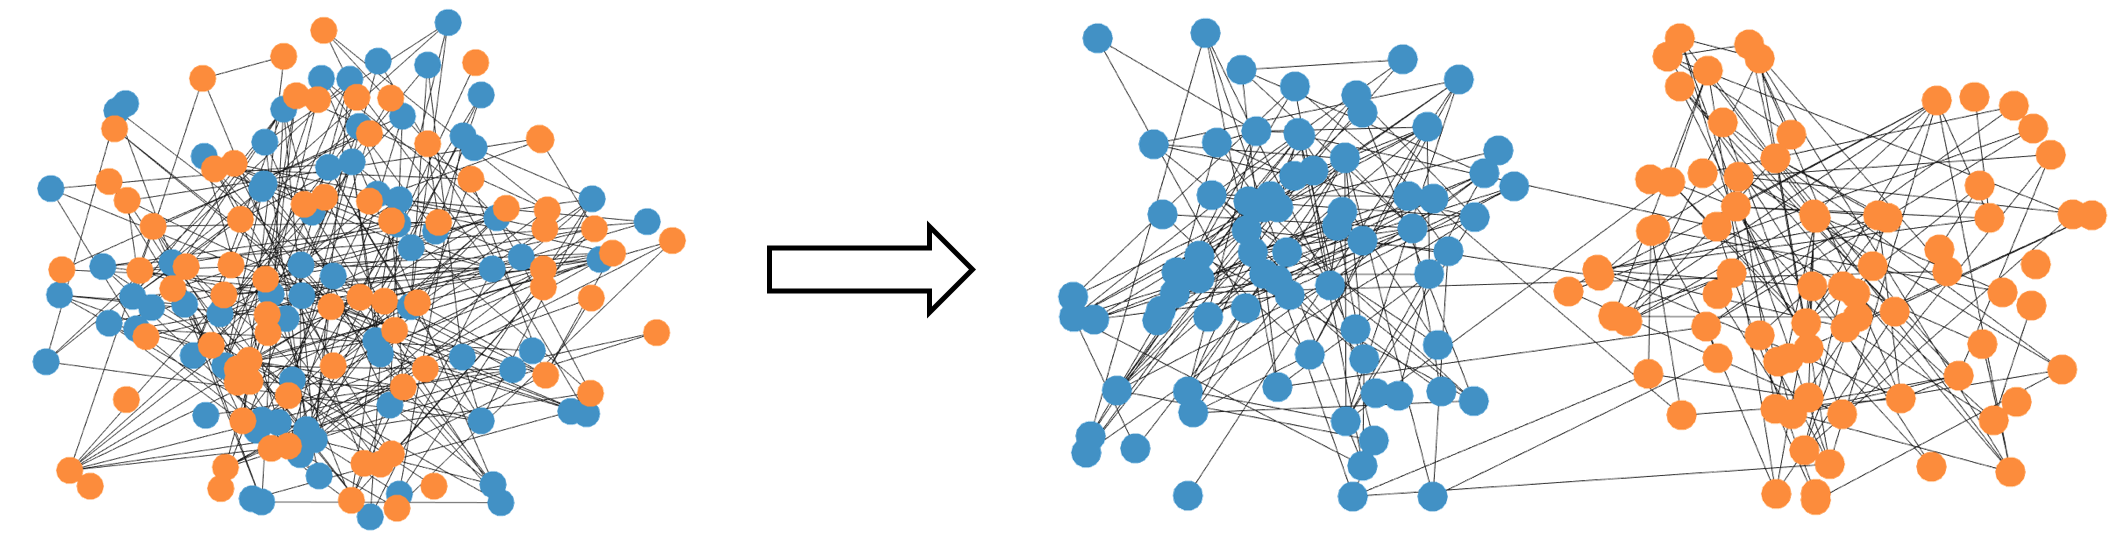
\includegraphics[width=0.85\textwidth]{figures/SBM_illustrate.png}
\end{center}
\caption{Illustration of graph clustering and community recovery, where one wishes to cluster all nodes into two communities based on the edges in the graph.} \label{fig:community}
\end{figure}


Next, we move on to a central problem that permeates data science applications: clustering. An important formulation that falls under this category is graph clustering or community recovery, which aims to cluster individuals into different communities based on  pairwise measurements of their relationships, each of which reveals information about whether or not two individuals belong to the same community \citep{abbe2017community}; see Figure~\ref{fig:community} for an illustration. There has been a recent explosion of interest in this problem, due to its wide applicability in, say, social network analysis \citep{azaouzi2019community}, image segmentation \citep{browet2011community}, shape mapping in computer vision \citep{huang2013consistent}, haplotype phasing in genome sequencing \citep{chen2016community}, to name just a few.
This section explores the capability of spectral methods in application to graph clustering;
 we will revisit the clustering problem again in Section~\ref{sec:Gaussian-mixture} for another common formulation.



\subsection{Problem formulation and assumptions}
\label{sec:setup-community-detection}


In this section, we formulate the graph clustering problem via the well-renowned {\em stochastic block model} (SBM) introduced in \citet{holland1983stochastic}---an idealized generative model that commonly serves as a  theoretical benchmark for evaluating community recovery algorithms.




Consider an undirected graph $\mathcal{G}=(\mathcal{V},\mathcal{E})$ that comprises $n$ vertices, where $\mathcal{V}$ and   $\mathcal{E}$ denote the vertex set and the edge set of $\mathcal{G}$, respectively.  The $n$ vertices, labelled by $1,\cdots, n$,
exhibit  community structures and can be grouped into two non-overlapping communities of {\em equal} sizes. Here and throughout,  $n$ is assumed to be an even number, so that each community contains exactly $n/2$ vertices.
To encode the community memberships, we assign $n$ binary-valued variables $x_i^{\star} \in \{1,-1\}$ ($1\leq i \leq n$) to the  vertices in a way that
%
\begin{align*}
	x_i^{\star} = \begin{cases} 1, \qquad & \text{if vertex } i \text{ belongs to the 1st community}, \\
				   -1, \quad  & \text{otherwise}. \end{cases}
\end{align*}
%




The SBM assumes that the set $\mathcal{E}$ of (undirected) edges  is generated randomly based on the community memberships of the incident vertices. To be precise, each pair $(i,j)$ of vertices  is  connected by an edge independently with probability $p$ (resp.~$q$) if $i$ and $j$ belong to the same community (resp.~different communities). The resultant connectivity pattern is represented by an adjacency matrix
$\bm{A}=[A_{i,j}]_{1\leq i,j\leq n}\in \{0,1\}^{n\times n}$, such that for each pair $(i,j)$,
%
\begin{align}
	A_{i,j} = \begin{cases} 1, \qquad & \text{if }(i,j)\in \mathcal{E}, \\ 0, & \text{otherwise}.   \end{cases}
\end{align}
%
By convention, we take the diagonal entries to be $A_{i,i}=0$ for all $1\leq i\leq n$. As a remark, the matrix $\bm{A}$ is symmetric since $\mathcal{G}$ is an undirected graph,  with upper triangular elements being realizations of independent Bernoulli random variables with mean either $p$ (if two nodes are in the same community) or $q$ (otherwise).  In addition, it is assumed throughout that $p>q>0$, implying that there are in expectation more within-community edges than across-community edges.

Based on the adjacency matrix $\bm{A}$ generated by the SBM,
the goal is to identify the latent community memberships of the vertices. To phrase it in mathematical terms,
the aim is to reconstruct the vector  $\bm{x}^{\star}=[x_i^{\star}]_{1\leq i\leq n}\in \{1,-1\}^n$ modulo the global sign,
namely, recovering either $\bm{x}^{\star}$ or $-\bm{x}^{\star}$.
This is all one can hope for, as there is
absolutely no basis to distinguish the names of two groups.
%$\bm{x}^{\star}$ from $-\bm{x}^{\star}$ given merely the edge information.




\subsection{Algorithm: spectral clustering}
\label{sec:algorithm-community-detection}

Now we describe a spectral method.
To simplify presentation, it is assumed without loss of generality that: $x_i^{\star}=1$ for any $1\leq i\leq n/2$, and $x_i^{\star}=-1$ for any $i > n/2$.


A starting point for the algorithm design is to examine the mean of the adjacency matrix,  given as follows
%
\begin{align*}
	 \mathbb{E}[\bm{A}]  	=
	\left[\begin{array}{cc}
		p\,\bm{1}_{n/2}\bm{1}^{\top}_{n/2} & q\,\bm{1}_{n/2}\bm{1}^{\top}_{n/2}\\
		q\,\bm{1}_{n/2}\bm{1}^{\top}_{n/2} & p\,\bm{1}_{n/2}\bm{1}^{\top}_{n/2}
	\end{array}\right] -   p \bm{I}.
\end{align*}
%
As revealed by the above calculation,   the  matrix constructed below
%
\begin{align}
	\bm{M} = \bm{A} -\frac{p+q}{2} \bm{1}_n\bm{1}^{\top}_n  + p\bm{I}
	\label{eq:M-data-matrix-SBM}
\end{align}
%
exhibits an approximate rank-1 structure, in the sense that its mean
%
\begin{align} \label{eq:M-data-matrix-expectation-SBM}
	\bm{M}^{\star} \coloneqq \mathbb{E}[\bm{M}] =
	\frac{p-q}{2}\left[\begin{array}{c}
		\bm{1}_{n/2}\\
		-\bm{1}_{n/2}
	\end{array}  \right] \left[\begin{array}{cc}
\bm{1}^{\top}_{n/2} & -\bm{1}^{\top}_{n/2}\end{array}\right]
\end{align}
%
is a rank-1 matrix.  The leading eigenvalue of $\bm{M}^{\star}$ and its associated eigenvector are given respectively by
%
\begin{align}
	\lambda^{\star}\coloneqq\frac{(p-q)n}{2},  
	\quad \text{and} \quad
	\bm{u}^{\star}  \coloneqq \frac{1}{\sqrt{n}}
	\left[\begin{array}{c}
		\bm{1}_{n/2}\\
		-\bm{1}_{n/2}
	\end{array}\right].
	\label{eq:leading-evalue-evector-M-SBM}
\end{align}
%
Crucially, the eigenvector  $\bm{u}^{\star}$ encapsulates the precise community structure we seek to recover: all positive entries of $\bm{u}^{\star}$ correspond to vertices from one community, while the remaining ones form another community.



Inspired by the above calculation, a candidate spectral clustering algorithm consists of eigendecomposition followed by entrywise rounding:
%
\begin{itemize}
	\item[1.] Compute the leading eigenvector $\bm{u}$ of  $\bm{M}$ (constructed in \eqref{eq:M-data-matrix-SBM});
	\item[2.] Compute the estimate $\bm{x}=[x_i]_{1\leq i\leq n}$  such that for any $1\leq i\leq n$,
	%
	\begin{align}
		  x_{i}= \mathsf{sgn}(u_i)  =
		  \begin{cases}
1,\quad & \text{if }u_{i}>0,\\
-1, \quad & \text{if }u_i \leq 0.
\end{cases}
	\end{align}
\end{itemize}
%
% Here, for any $z\in \mathbb{R}$, the sign function obeys $\mathsf{sgn}(z)=1$ if $z>0$ and $\mathsf{sgn}(z)=-1$ otherwise. 
In words, the community memberships are estimated in accordance with the signs of the entries of the leading eigenvector of $\bm{M}$, namely, the entries with the same signs are declared to come from the same cluster.

%which has two non-vanishing eigenvalues and their associated eigenvectors
%$$
%  	\lambda_1^* = \frac{(p+q)n}{2},~\lambda_2^* = \frac{(p-q)/n}{2},  \mbox{ and }  \bu_1^* = \frac{1}{\sqrt{n}}\mathbf{1}, ~ 	\bu_2^*=\frac{1}{\sqrt{n}}\left[\begin{array}{c}
%  		\bm{1}_{n/2}\\
%  		-\bm{1}_{n/2}
%  	\end{array}  \right ].
%$$
%Therefore, the second eigenvector reveals the true membership of the community.  We can work directly with the second eigenvector, but we here work with the first eigenvector by shifting the first component $\lambda_1^* \bu_1^*  (\bu_1^* )^T$  in the eigen-decomposition.  

\begin{remark}
	The above algorithm requires prior knowledge of the parameters $p$ and $q$ when constructing  $\bm{M}$. It is also feasible to develop a ``model-agnostic'' alternative by, for instance, looking at the second eigenvector of $\bm{A}$ (since the second eigenvector of $\mathbb{E}[\bm{A}]$ turns out to be precisely $\bm{u}^{\star}$), which does not rely on prior information about $p$ and $q$ at all; see, e.g., \citet{abbe2020entrywise} for details.  Here, we adopt the above model-dependent version primarily for convenience of exposition.  %To make the method feasible, we note that $ \mathbb{E} \sum_{i,j} A_{i, j} = n^{2}(p+q)/2 - n p$ and we can estimate $p+q$ by $2n^{-2} \sum_{i,j}A_{i,j}$ in the construction of $M$.
\end{remark}


\subsection{Performance guarantees: almost exact recovery}
\label{sec:theory-community-detection}

The spectral method enjoys appealing statistical guarantees for recovering the community structure of the SBM, which can be readily obtained by invoking the $\ell_2$ eigenvector perturbation theory.  To demonstrate this, we begin by developing an upper bound on the spectral norm of the perturbation matrix $\bm{E}\coloneqq \bm{M} - \bm{M}^{\star}$,
postponing the proof to Section~\ref{sec:proof-auxiliary-lemmas-community-detection}.
%
\begin{lemma} \label{lemma:E-spectral-norm-SBM}
	Consider the settings in Section~\ref{sec:setup-community-detection}, and suppose that $np\gtrsim \log n$. Then with probability at least $1-O(n^{-8})$, one has
	%
	\begin{align}
		\| \bm{E} \| \lesssim \sqrt{np} .
	\end{align}
\end{lemma}
%
This spectral norm bound, in conjunction with the Davis-Kahan sin$\bm{\Theta}$ theorem, leads to the following theoretical support for the spectral method introduced in Section~\ref{sec:algorithm-community-detection}.
%
\begin{theorem}
	\label{thm:community-detection-weak}
	Consider the setting in Section~\ref{sec:setup-community-detection}, and suppose that
	%
	\begin{align}
		p \gtrsim\frac{\log n}{n}, 
		\qquad\text{and}\qquad \sqrt{\frac{p}{n}} =o(p-q).
		\label{eq:assumption-p-q-SBM-L2}
	\end{align}
	With probability exceeding $1-O(n^{-8})$, the spectral method achieves
	%
	\begin{align*}
		\frac{1}{n}\sum_{i=1}^{n}\mathbbm1\big\{ x_{i} = x_{i}^{\star}\big\} = 1- o(1), 
		\quad \text{or} \quad
		\frac{1}{n}\sum_{i=1}^{n}\mathbbm1\big\{ x_{i} = - x_{i}^{\star}\big\} = 1- o(1) .
	\end{align*}
	%
\end{theorem}
%
It is noteworthy that the metric
%
\[
	\min \Bigg\{  \frac{1}{n}\sum_{i=1}^{n}\mathbbm1\big\{ x_{i} \neq x_{i}^{\star}\big\},\, \frac{1}{n}\sum_{i=1}^{n}\mathbbm1\big\{ x_{i} \neq - x_{i}^{\star}\big\} \Bigg\}
\]
%
can be understood as the mis-clustering rate.
In a nutshell, Theorem~\ref{thm:community-detection-weak} asserts that with the assistance of simple rounding (i.e., the $\mathsf{sgn}(\cdot)$ operation), the spectral method allows for {\em almost} exact community recovery---namely, correctly clustering all but a vanishing fraction of the vertices---assuming satisfaction of Condition~\eqref{eq:assumption-p-q-SBM-L2}.  Note that ``almost exact recovery'' is also referred to as ``weak consistency'' in the literature \citep{abbe2017community}.


Let us take a moment to interpret the recovery condition in \eqref{eq:assumption-p-q-SBM-L2}.
The first requirement  in Condition~\eqref{eq:assumption-p-q-SBM-L2} ensures the presence of sufficiently many edges  in the observed graph, while still permits the graph to be fairly sparse (with average vertex degrees as low as the order of $\log n$).
The second  requirement in Condition~\eqref{eq:assumption-p-q-SBM-L2}---which imposes a lower bound on the separation  between  the edge densities $p$ and $q$---guarantees that the within-community edges can be
adequately differentiated from across-community edges. As a more concrete example, consider the scenario where $p\asymp (\log n)/{n}$
(so that each vertex is only expected to be incident to $O(\log n)$ edges).
In this case, the second requirement in Condition~\eqref{eq:assumption-p-q-SBM-L2} can be translated into
%
\begin{align*}
	p-q \gg {\sqrt{\log n}}\,/\,{n}, \qquad \text{if } p\asymp  (\log n)\,/\,n.
\end{align*}
%
This indicates that the separation  $p-q$ is allowed to be considerably smaller than the edge densities, even in this low-edge-density regime.
In comparison, in another extreme case with $p \asymp 1$ (so that each vertex is likely to be connected with a constant fraction of other vertices), the second requirement in Condition~\eqref{eq:assumption-p-q-SBM-L2} reads
%
\begin{align*}
	p-q \gg 1/\sqrt{n} , \qquad \text{if } p \asymp  1,
\end{align*}
%
thereby allowing the edge density difference to be even $\sqrt{n}$ times smaller than the edge densities themselves.


It is worth highlighting that the spectral method is not merely capable of correctly clustering all but a diminishing fraction of vertices;
in fact, it allows for simultaneous and exact recovery for {\em all} vertices under slightly modified conditions. Establishing this stronger assertion requires developing a significantly strengthened $\ell_{\infty}$-based eigenvector perturbation theory, which will be elucidated in Section~\ref{sec:community-detection-linf}.
The discussion about the statistical optimality of this spectral method is  postponed to Section~\ref{sec:community-detection-linf} as well.



\paragraph{Proof of Theorem~\ref{thm:community-detection-weak}.}
%
It is readily seen from Lemma \ref{lemma:E-spectral-norm-SBM} that with with probability at least  $1-O(n^{-8})$,
%
\[
	\|\bm{E}\| \leq \Big(1-\frac{1}{\sqrt{2}}\Big) \frac{n(p-q)}{2}  = \Big(1-\frac{1}{\sqrt{2}}\Big) \lambda^{\star},
\]
%
provided that Condition~\eqref{eq:assumption-p-q-SBM-L2} holds. Here, $\lambda^{\star}$ is defined in \eqref{eq:leading-evalue-evector-M-SBM}. Apply Corollary~\ref{cor:davis-kahan-conclusion-corollary} to yield that with probability at least  $1-O(n^{-8})$,
%
\begin{align}
	\mathsf{dist}\big(\bm{u},\bm{u}^{\star}\big)\leq\frac{2\|\bm{E}\|}{\lambda^{\star}}\lesssim\frac{\sqrt{np}}{n(p-q)}	=o(1),
	\label{eq:L2-bound-u-ustar-CD-L2}
\end{align}
%
where the last relation follows from Condition \eqref{eq:assumption-p-q-SBM-L2}.


Assume, without loss of generality, that $\|\bm{u}-\bm{u}^{\star}\|_{2}=\mathsf{dist}\big(\bm{u},\bm{u}^{\star}\big)$.
We shall pay attention to the set
%
$$
	\mathcal{N}\coloneqq \big\{ i\mid |u_{i}-u_{i}^{\star}| \geq {1}/{\sqrt{n}}\big\}.
$$
%
In view of the rounding procedure: for any $i$ obeying $x_{i}\neq x_{i}^{\star}$, one necessarily has $\mathsf{sgn}(u_{i})\neq \mathsf{sgn}(u_{i}^{\star})$,
thus indicating that $|u_i - u_{i}^{\star}| \geq |u_{i}^{\star}| = 1/\sqrt{n}$ and hence $i\in \mathcal{N}$.
Combining the $\ell_2$ bound \eqref{eq:L2-bound-u-ustar-CD-L2} and the definition of $\mathcal{N}$, we can easily verify that
%
\[
|\mathcal{N}|\leq\frac{\|\bm{u}-\bm{u}^{\star}\|_{2}^{2}}{(1/\sqrt{n})^{2}}=o\big(n\big),
\]
%
which in turn leads to the advertised result
%
\[
	\frac{1}{n}\sum_{i=1}^{n} \mathbbm{1} \big\{ x_{i}\neq x_{i}^{\star}\big\}
	\leq \frac{1}{n}\sum_{i=1}^{n} \mathbbm{1} \Bigg \{ |u_i - u_{i}^{\star}| \geq \frac{1}{\sqrt{n}} \Bigg\}
	= \frac{|\mathcal{N}|}{n}=o(1) .
\]
%
%\end{proof}



\subsection{Proof of Lemma~\ref{lemma:E-spectral-norm-SBM}}
\label{sec:proof-auxiliary-lemmas-community-detection}


We intend to apply Theorem~\ref{thm:tighter-spectral-normal-ramon} to establish this lemma.
First, observe from the definition $\bm{E}=\bm{M}-\bm{M}^{\star}=\bm{A}-\mathbb{E}[\bm{A}]$ that
%
\[
	\big|E_{i,j}\big|\leq  \max_{i,j}\big|A_{i,j}\big| = 1.
\]
%
In addition, the variance of $E_{i,j}$ is upper bounded by
%
\begin{align*}
	 \mathbb{E}\big[E_{i,j}^{2}\big]  = \mathsf{Var}(A_{i,j})
	 \leq \mathbb{E}\big[A_{i,j}^{2}\big]
 	 \overset{(\mathrm{i})}{\leq}\max\{p,q\}\overset{(\mathrm{ii})}{=} p
\end{align*}
%
for any $(i,j)$,
where %(i) is valid since $E_{i,j}$ and $A_{i,j}$ differ only by a constant offset,
%(ii) holds since $\mathsf{Var}(A_{i,j})\leq \mathbb{E}[A_{i,j}^2]$,
(i) follows since $A_{i,j}$ is a Bernoulli random variable with mean either $p$ or $q$, and (ii) is due to the assumption $p>q$.
The bound \eqref{eq:X-spectral-norm-iid-special-ramon} and the condition $np\gtrsim \log n$ thus imply that
%
\begin{align}
	\|\bm{E}\|= \big\| \bm{M} - \mathbb{E}[\bm{M}] \big\| \lesssim \sqrt{np} + O(\sqrt{\log n}) \asymp \sqrt{np}
\end{align}
%
with probability exceeding $1-O(n^{-8})$.

\section{Clustering in Gaussian mixture models}
\label{sec:Gaussian-mixture}


% We now revisit an important task in unsupervised learning---clustering, which aims to group unlabeled data points into a few clusters (so that the data within the same cluster share similar characteristics). 



This section is also concerned with clustering, with the aim of grouping unlabeled data points into a few clusters (so that the data within the same cluster share similar characteristics). 
In contrast to the graph clustering setting in Section~\ref{sec:community-detection} where only pairwise measurements are available, this section  assumes direct access to data samples for each individual. Spectral methods---possibly with the aid of subsequent refinement like $k$-means---continue to be remarkably effective  for this setting,  achieving practical success in, say, image segmentation \citep{shi2000normalized}, text separation \citep{reynolds1995robust}, climate modeling \citep{lin2017statistical}, and heterogeneity modeling in precision medicine and marketing \citep{fan2014challenges}. Motivated by the empirical successes, understanding the theoretical properties of spectral clustering has garnered growing attention recently. In particular, Gaussian mixture models emerge as a succinct model of attack,  providing elegant yet intuitive abstractions to pivotal quantities that dictate the feasibility of  spectral clustering.


%

\subsection{Gaussian mixture models and assumptions}
\label{sec:setup-gaussian-mixture}

\paragraph{Model and goal.}
Imagine that we have collected $n$ independent samples $\{\bm{x}_{i}\}_{1\leq i\leq n}$,
generated from a mixture of $r$ spherical Gaussians with respective centers $\bm{\theta}_{1}^{\star},\cdots,\bm{\theta}_{r}^{\star}\in\mathbb{R}^{p}$.
More precisely, for each sample vector $\bm{x}_{i}\in\mathbb{R}^{p}$, we assume the existence of a predetermined, yet {\em a priori} unknown,
cluster membership variable $\xi_{i}^{\star}\in [r]$ such that
%
\begin{equation}
\bm{x}_{i}=\begin{cases}
\bm{\theta}_{1}^{\star}+\bm{\eta}_{i},\qquad & \text{if }\xi_{i}^{\star}=1,\\
\quad\,\,\vdots & \quad\,\vdots\\
\bm{\theta}_{r}^{\star}+\bm{\eta}_{i}, & \text{if }\xi_{i}^{\star}=r,
\end{cases}\label{eq:data-model-r-Gaussian-GM}
\end{equation}
%
where the noise vector $\bm{\eta}_{i}\sim\mathcal{N}(\bm{0},\bm{I}_{p})$ is independently generated across the samples.
In words, $\xi_{i}^{\star}$ indicates which Gaussian component a sample is generated from.
Clustering in this Gaussian mixture model can, therefore,
be posed as recovering the set of cluster membership variables $\{\xi_{i}^{\star}\}_{1\leq i\leq n}$ (modulo the global permutation ambiguity).


\paragraph{Assumptions.} To simplify our exposition, we impose the following assumptions throughout this section. As a worthy note,  this assumption is often non-essential and can be significantly relaxed, which we shall remark on momentarily in Remark~\ref{remark:assumptions_gmm}.
%
\begin{assumption}
	\label{assumption:gaussian-mixture}
	The centers are independently generated obeying
	%
	\[
		\bm{\theta}_{i}^{\star} ~\overset{\mathrm{i.i.d.}}{\sim}~ \mathcal{N}\Bigg( \bm{0}, \frac{\Delta^2}{2p} \bm{I}_p \Bigg),
		\qquad 1\leq i\leq r
	\]
 	%
	for some parameter $\Delta>0$.
\end{assumption}
%
Under this assumption, standard Gaussian concentration inequalities  \citep{vershynin2016high} tell us that, with high probability (for large $p$ and $n=\mathrm{poly}(p)$),
%
\begin{align*}
& ~~~~~~ \big\|\bm{\theta}_{i}^{\star}\big\|_{2}^{2}  =(1+o(1))\frac{\Delta^{2}}{2},
\quad~~
\big|\bm{\theta}_{i}^{\star\top}\bm{\theta}_{j}^{\star}\big|= o(\Delta^2), \\
%O\left(\Delta\sqrt{\frac{\log n}{p}}\right),\\
& \big\|\bm{\theta}_{i}^{\star}-\bm{\theta}_{j}^{\star}\big\|_{2}^{2}
=\big\|\bm{\theta}_{i}^{\star}\big\|_{2}^{2}+\big\|\bm{\theta}_{j}^{\star}\big\|_{2}^{2}-2\bm{\theta}_{i}^{\star\top}\bm{\theta}_{j}^{\star}=(1+o(1))\Delta^{2}
\end{align*}
%
hold for any pair $i\neq j$, where $o(1)$ denotes a vanishingly small quantity as $p$ approaches infinity. The indication is that the parameter $\Delta$ reflects (approximately) the separation between any pair of centers.


For simplicity of presentation, it is further assumed that there are exactly $n/r$ samples drawn from each of the $r$ Gaussian components.
Without loss of generality, we assume that
%
\begin{align}
	\xi_{i}^{\star}=l,\qquad\text{if }\left\lceil \frac{\,i\,}{r}\right\rceil =l
	\label{eq:zi-assignment-GM}
\end{align}
%
for any $1\leq i\leq n$, where the ceiling function $\lceil x \rceil$ represents the least integer greater than or equal to the number $x\in \mathbb{R}$.
%the ceiling operator such as  $\left\lceil .01 \right\rceil = 1$ and $ \left\lceil 2.2 \right\rceil = 3$.
In other words, the first batch of $n/r$ samples is drawn from the first Gaussian component, the second batch comes from the second component, and so on.
It is worth pointing out that this assumed assignment information \eqref{eq:zi-assignment-GM} is unavailable when running the spectral clustering algorithm.




\subsection{Algorithm and rationale}
\label{sec:algorithm-gaussian-mixture}


\paragraph{Motivation: spectral structure of the data matrix.}

In order to develop a spectral clustering algorithm, it is instrumental to first examine the spectral feature of the following data matrix
%
\begin{align}
	\bm{X}\coloneqq[\bm{x}_{1},\cdots,\bm{x}_{n}]=\mathbb{E}[\bm{X}]+\underset{\eqqcolon\,\bm{Z}}{\underbrace{[\bm{\eta}_{1},\cdots,\bm{\eta}_{n}]}}.
	\label{eq:defn-Z-X-EX-GMM}
\end{align}
%
Clearly, $\mathbb{E}[\bm{X}] \in \mathbb{R}^{p \times n}$ exhibits a rank-$r$ structure:
%
\begin{align*}
	\mathbb{E}[\bm{X}] & =\big[\bm{\theta}_{1}^{\star},\cdots,\bm{\theta}_{1}^{\star},\bm{\theta}_{2}^{\star},\cdots,\bm{\theta}_{2}^{\star},\cdots,\bm{\theta}_{r}^{\star},\cdots,\bm{\theta}_{r}^{\star}\big]
 	= \bm{\Theta}^{\star}\bm{F}^{\star\top},
\end{align*}
%
where we define
%
\begin{align}
\bm{\Theta}^{\star}\coloneqq\left[\bm{\theta}_{1}^{\star},\cdots,\bm{\theta}_{r}^{\star}\right] \in \mathbb{R}^{p\times r},
\quad
%\text{and}\quad
\bm{F}^{\star}\coloneqq {\footnotesize\left[\begin{array}{cccc}
\bm{1}_{\frac{n}{r}}\\
 & \bm{1}_{\frac{n}{r}}\\
 &  & \ddots\\
 &  &  & \bm{1}_{\frac{n}{r}}
\end{array}\right] }\in \mathbb{R}^{n\times r}.
\label{eq:defn-Theta-star-F-star-GMM}
\end{align}
%


Similarly, the Gram matrix $\bm{X}^{\top}\bm{X}$ also inherits this rank-$r$ structure in the following sense (albeit in the form of a ``spiked'' structure due to the presence of noise):
%
\begin{align}
	\mathbb{E}\big[\bm{X}^{\top}\bm{X}\big]
	& =\mathbb{E}[\bm{X}]^{\top}\mathbb{E}[\bm{X}]+\mathbb{E}\big[\bm{Z}^{\top}\bm{Z}\big]
	=\bm{F}^{\star}\bm{\Theta}^{\star\top}\bm{\Theta}^{\star}\bm{F}^{\star\top}+p\bm{I}_n .
	\label{eq:mean-XT-X-GM}
\end{align}
%
Recognizing that  $\bm{F}^{\star}$ encodes all the cluster membership information,
one is motivated to attempt information extraction from the rank-$r$ eigenspace of $\bm{X}^{\top}\bm{X}$,
akin to the PCA algorithm introduced in Section~\ref{sec:algorithm-PCA}.



\paragraph{Algorithm: spectral clustering followed by $k$-means.}

With the preceding spectral properties in mind, we are ready to present a spectral clustering algorithm tailored to this Gaussian mixture model.
Given that the eigenspace of $\bm{X}^{\top}\bm{X}$ might only approximate $\bm{F}^{\star}$ up to global rotation,
we include a follow-up $k$-means scheme \citep{macqueen1967some}
 to produce a valid clustering outcome based on the spectral estimate.
%
\begin{itemize}
	\item[1.] Compute the leading rank-$r$ eigenspace $\bm{U}\in \mathbb{R}^{n\times r}$ of $\bm{X}^{\top}\bm{X}$.

	\item[2.] Compute $\bm{Y}= \mathcal{P} \big( \bm{U}\bm{U}^{\top} \big) \in \mathbb{R}^{n\times n}$,
		where the operator $\mathcal{P}(\cdot)$ projects each column onto the unit sphere,
		i.e., 
	%
\begin{align*}
	%\label{eq:projection-unit-ball-GMM}
	\mathcal{P}(\bm{Z}) \coloneqq \Big[ \frac{\bm{z}_{1}}{\|\bz_1\|_2},\cdots,  \frac{\bz_n}{\|\bm{z}_{n}\|_2}\Big] 
\end{align*}
	%
% Clearly, the global scaling factor $\sqrt{n/r}$ is not needed.
	for any matrix $\bm{Z}=[\bm{z}_1,\cdots,\bm{z}_n]$. 
	As will be discussed below, the projection step is not necessary, and we can also simply take $\bY = \bU \bU^\top$.
		%,  but improves somewhat the  performance; see \eqref{eq:Y-Ystar-dist-GMM} below in the proof. \yxc{check}
	
	
	
	\item[3.] Let $\bm{y}_i$ represent the $i$-th column of $\bm{Y}$, and apply the $k$-means algorithm
	(with $k=r$) to the vectors $\{\by_i\}_{1 \leq i \leq n}$  to find the cluster centers and cluster labels for all individuals; namely, we  compute
%
\begin{equation}
\Big(\big\{\widehat{\xi}_{i}\big\}_{i=1}^{n},\big\{\widehat{\bm{\vartheta}}_{i}\big\}_{i=1}^{r}\Big)
= \hspace{-0.2em}
\underset{\xi_{1},\cdots,\xi_{n}\in[r],\,\bm{\vartheta}_{1},\cdots,\bm{\vartheta}_{r}\in\mathbb{R}^{n}}{\arg\min}\sum_{i=1}^{n}\big\|\bm{y}_{i}-\bm{\vartheta}_{\xi_{i}}\big\|_{2}^{2} .
\label{eq:k-means-GMM}
\end{equation}
%
%The $k$-mean algorithm alternatively optimizes $\big\{\xi_{i}\big\}_{i=1}^{n}$  given $\big\{\bm{\vartheta}_{i}\big\}_{i=1}^{r}$ and  $\big\{\bm{\vartheta}_{i}\big\}_{i=1}^{r}$ given $\big\{\xi_{i}\big\}_{i=1}^{n}$.  Given the current estimate of centers $\big\{\widehat{\bm{\vartheta}}_{i}\big\}_{i=1}^{r}$, classify $\bm{x}_i$ to its nearest estimated center, i.e., assign $\widehat{\xi}_{i}$ to the label of that of the nearest center ; and given the class labels $\big\{\widehat{\xi}_{i}\big\}_{i=1}^{n}$, use the sample means of the clusters to update  $\big\{\widehat{\bm{\vartheta}}_{i}\big\}_{i=1}^{r}$.  The initialization is typically $r$ randomly selected data points.  Since the optimization is non-convex, multiple random initializations are used and the optimal output, in terms of target function \eqref{eq:k-means-GMM}, is used as the final estimate.
\end{itemize}
%
The algorithm then returns $\big\{\widehat{\xi}_{i}\big\}_{1\leq i\leq n}$ as the clustering result.
Interestingly, Step 1 bears similarity with the spectral algorithm for graph clustering,
since  we essentially generate a pairwise similarity measurement for each pair $(i,j)$ using the inner product $\langle \bm{x}_i, \bm{x}_j \rangle$.

\begin{remark}
	The $k$-means formulation \eqref{eq:k-means-GMM}---which minimizes the sum of squared distance between each data point and the center of its associated cluster---is
	an integer program and intractable in general \citep{aloise2009np}.
	Fortunately, computationally feasible solutions are available either under sufficient minimum center separation or when suitably initialized
	\citep{lloyd1982least,vempala2004spectral,lu2016statistical,peng2007approximating,awasthi2015relax,mixon2017clustering,iguchi2017probably}.
	An in-depth account of this computational aspect is beyond the scope of this monograph,
	and the interested reader is referred to \citet{li2020birds,loffler2019optimality} for details.
\end{remark}


%\citep{peng2007approximating,awasthi2015relax,mixon2017clustering,iguchi2017probably,li2020birds}



\paragraph{Further explanations.}

We take a moment to explain why $k$-means is applied to the columns of $\bm{Y}$.
Recall that the central object the spectral algorithm seeks to approximate
is the leading rank-$r$ eigenspace of $\bm{F}^{\star}\bm{\Theta}^{\star\top}\bm{\Theta}^{\star}\bm{F}^{\star\top}$ (cf.~\eqref{eq:mean-XT-X-GM}).
For convenience, suppose we have the eigendecomposition  $\bm{\Theta}^{\star\top}\bm{\Theta}^{\star}=\bm{U}_{\theta}\bm{\Sigma}_{\theta}\bm{U}_{\theta}^{\top}$,
where $\bm{U}_{\theta}\in\mathcal{O}^{r\times r}$ is  orthonormal and $\bm{\Sigma}_{\theta}\in\mathbb{R}^{r\times r}$ is diagonal.
This results in the decomposition
%
\begin{equation}
\bm{F}^{\star}\bm{\Theta}^{\star\top}\bm{\Theta}^{\star}\bm{F}^{\star\top}=\frac{n}{r}\cdot\Big(\underset{\eqqcolon\,\bm{U}^{\star}}{\underbrace{\sqrt{\frac{r}{n}}\bm{F}^{\star}\bm{U}_{\theta}}}\Big)\bm{\Sigma}_{\theta}\Big(\sqrt{\frac{r}{n}}\bm{F}^{\star}\bm{U}_{\theta}\Big)^{\top}.
\label{eq:FTheta-Theta-F-eigenspace}
\end{equation}
%
Apparently, the matrix $\bm{U}^{\star}\in\mathbb{R}^{n\times r}$ defined above has orthonormal columns and, as a result,
represents the eigenspace of $\bm{F}^{\star}\bm{\Theta}^{\star\top}\bm{\Theta}^{\star}\bm{F}^{\star\top}$.
The idea is that if the spectral estimate $\bm{U}$ approximates $\bm{U}^{\star}\in\mathbb{R}^{n\times r}$ well,
then the matrices $\sqrt{\frac{n}{r}} \, \bm{U}\bm{U}^{\top}$ and $\bm{Y}$ constructed above are hopefully close to the following matrix
%
\begin{equation}
\bm{Y}^{\star}  \coloneqq  \sqrt{\frac{n}{r}} \, \bm{U}^{\star}\bm{U}^{\star\top}
%=\bm{F}^{\star}\bm{U}_{\theta}\bm{U}_{\theta}^{\top}\bm{F}^{\star\top}
%= \sqrt{\frac{r}{n}} \, \bm{F}^{\star}\bm{F}^{\star\top}
= \sqrt{\frac{r}{n}} \left[\begin{array}{ccc}
\bm{1}_{\frac{n}{r}}\bm{1}_{\frac{n}{r}}^{\top}\\
 & \ddots\\
 &  & \bm{1}_{\frac{n}{r}}\bm{1}_{\frac{n}{r}}^{\top}
\end{array}\right].
\label{eq:Ystar-definition-GMM}
\end{equation}
%
As can be easily seen, the data points belonging to the same ground-truth cluster are associated with identical columns in $\bm{Y}^{\star}$;
for instance, each of the first $n/r$ samples---which belongs to the first cluster---corresponds to a column of $\bm{Y}^{\star}$ given by
$\sqrt{\frac{r}{n}}\,  {\scriptsize \left[\begin{array}{c}
\bm{1}_{n/r}\\
\bm{0}
\end{array}\right]}$.
%
Therefore, clustering  the columns of $\bm{Y}$ via $k$-means is expected to unveil the underlying cluster structure,
provided that $\bm{Y}$ is sufficiently close to $\bm{Y}^{\star}$.
In summary,  spectral estimation (Steps 1-2) effectively leads to a new vector $\bm{y}_i$ for each point, which enjoys substantially enhanced signal-to-noise ratio compared to $\bm{x}_i$ and boosts the chance for $k$-means to succeed.


We shall also explain the projection operation enforced in Step 2 of the algorithm.
Given that each column of $\bm{Y}^{\star} $ has unit $\ell_2$ norm, projecting each column of  $ \bm{U}\bm{U}^{\top}$ onto the unit sphere ensures that no column of $\bm{Y}$ has an abnormal size.
Note, however, that this projection step is  non-essential and is introduced here 
primarily to simplify the mathematical analysis. Spectral clustering is expected to succeed even in the absence of such a projection step \citep{loffler2019optimality}.
% Yuxin: projection is actually needed in the proof to show that || y_i ||_2 \leq 1
% %with expectation of improved empirical performance.  Indeed, the proof goes through without this projection step; see \eqref{eq:Y-Ystar-dist-GMM}.



\begin{remark}
	Another variation of spectral clustering is to directly apply the $k$-means algorithm to cluster the rows of $\bU$ (or some properly rescaled version of them) \citep{loffler2019optimality}.  To explain the rationale, we note that under the assumption \eqref{eq:zi-assignment-GM}, $\bU^{\star}$ necessarily consists of $r$ blocks of identical rows as follows:
$$
	\bU^{\star} = \sqrt{\frac{r}{n}} \begin{pmatrix}
		\bm{1}_{n/r} \bm{\nu}_1^\top\\
   	\vdots\\
   	\bm{1} _{n/r} \bm{\nu}_r^\top
   \end{pmatrix} ,
$$
where $\bm{\nu}_1^\top, \cdots, \bm{\nu}_r^\top$ are the orthonormal rows of the matrix $\bU_\theta$ (cf.~\eqref{eq:FTheta-Theta-F-eigenspace}).
Consequently,  clustering the rows of $\bU^{\star}$ reveals exactly the true cluster assignments of all individuals.
The idea of our spectral analysis below applies to this method as well; we leave it to the reader as an exercise.
\end{remark}


\subsection{Performance guarantees}
\label{sec:theory-gaussian-mixture}


Now, we turn to characterizing the clustering performance of the above spectral algorithm.
We shall focus attention on the mis-clustering rate as the performance metric.  As the cluster labels in $[r]$ can be arbitrarily permuted,
the mis-clustering rate associated with the labels $\{\widehat{\xi}_{i}\}$ returned by our algorithm is defined as
%
\[
	\ell_{\mathsf{mis}}\big(\{\widehat{\xi}_{i}\},\{\xi_{i}^{\star}\}\big)
	\coloneqq \min_{\phi\in\Pi} ~ \frac{1}{n}\sum_{i=1}^{n}\mathbbm{1}\left\{ \phi(\widehat{\xi}_{i})\neq\xi_{i}^{\star}\right\} ,
\]
%
where $\Pi$ is the set of permutations of $[r]$.
In words, this metric captures the average number of mislabeled data points, after accounting for global permutation.
For notational convenience, we shall set $\bm{M}^{\star}\coloneqq\mathbb{E}\big[\bm{X}^{\top}\bm{X}\big]$ and
$\bm{E}\coloneqq\bm{X}^{\top}\bm{X} - \mathbb{E}\big[\bm{X}^{\top}\bm{X}\big]$ throughout this section.


The first step towards analyzing the statistical accuracy of the spectral algorithm lies in developing a perturbation bound on $\|\bm{U}\bm{U}^{\top} - \bm{U}^{\star}\bm{U}^{\star\top}\|$, where $\bm{U}^{\star}$ (cf.~\eqref{eq:FTheta-Theta-F-eigenspace}) represents the leading rank-$r$ eigenspace of $\bm{M}^{\star}$.
This can be accomplished via the Davis-Kahan theorem, which requires us to first control the size of the perturbation $\bm{E}$.
%
\begin{lemma}
	\label{lem:perturbation-norm-Gaussian-mixture}
	Consider the settings in Section~\ref{sec:setup-gaussian-mixture}, and suppose $p\gtrsim r \log ^3 (n+p)$.
	Then with probability at least $1-O((n+p)^{-10})$, one has
	%
	\begin{align*}
		\|\bm{E}\|  \lesssim\frac{\Delta n\sqrt{\log(n+p)}}{\sqrt{r}}+\sqrt{np\log(n+p)}+n\log^{2}(n+p) .
	\end{align*}
	%
\end{lemma}
%
%Another part that needs to be taken care of is developing a lower bound on the spectral gap of $\bm{M}^{\star}$.
%In view of \eqref{eq:mean-XT-X-GM} and \eqref{eq:FTheta-Theta-F-eigenspace}, the spectral gap of $\bm{M}^{\star}$ relies heavily on the spectral property of $\bm{\Theta}^{\star\top}\bm{\Theta}^{\star}$, which is studied through the following lemma.
%%
%\begin{lemma}
%	\label{lemma:sigma-min-Thetastar-GMM}
%	Consider the setting in Section~\ref{sec:setup-gaussian-mixture}, and suppose that  $p\geq C_{2}r^{2}\log p$ for some sufficiently large constant $C_2>0$.
%	Then with probability at least $1-O(p^{-8})$, the matrix $\bm{\Theta}^{\star}$ defined in \eqref{eq:defn-Theta-star-F-star-GMM} obeys
%	\[
%		\lambda_{\min}\big(\bm{\Theta}^{\star\top}\bm{\Theta}^{\star}\big) \geq \Delta^2 / 4.
%	\]
%\end{lemma}
%%

%
The proof of this lemma can be found in Section~\ref{sec:proof-auxiliary-lemmas-GM}.
Equipped with the above perturbation bound, we are ready to present our statistical guarantees for spectral clustering.
%
\begin{theorem}
	\label{thm:GMM-performance}
	Consider the setting and assumptions in Section~\ref{sec:setup-gaussian-mixture}, and suppose that $r=O(1)$ and $p\gtrsim \log^3 n$.
	% Suppose that  $\Delta\geq C_{1} \sqrt{r}\max \big\{ \big(\frac{p\log(n+p)}{n}\big)^{1/4}, \log(n+p) \big\}$ for some sufficiently large constant $C_1>0$.
	With probability at least $1-O(p^{-10})$, the mis-clustering rate of the spectral algorithm in Section~\ref{sec:algorithm-gaussian-mixture} achieves
	 $$ \ell_{\mathsf{mis}}\big(\{\widehat{\xi}_{i}\},\{\xi_{i}^{\star}\}\big) = o(1) ,$$
	with the proviso that
	%
	\begin{equation}
		\log(n+p)=o(\Delta)\quad\text{and}\quad\Big(\frac{p\log(n+p)}{n}\Big)^{1/4}=o(\Delta).
		\label{eq:condition-Delta-thm-GMM}
	\end{equation} 	
	%
\end{theorem}
%

Before embarking on the proof of this theorem, we discuss briefly the implications of this theorem.
 In order to ensure a vanishingly small mis-clustering rate, it suffices for the center separation $\Delta$ to exceed
%
\[
	\Delta\gtrsim \begin{cases}
		\mathrm{poly}\log(n+p), & \text{if }p\leq n,\\
		\big(\frac{p}{n}\big)^{1/4} \mathrm{poly}\log(n+p),\qquad & \text{if }p\geq n.
	\end{cases}
\]
%
This separation condition matches the minimax lower bound  up to some logarithmic term \citep{cai2018rate,ndaoud2018sharp}.
In particular,  in the high-dimensional case where $p\geq n$, the required separation condition changes fairly gracefully with the aspect ratio $p/n$.

\begin{remark}\label{remark:assumptions_gmm}
	As alluded to previously, Assumption \ref{assumption:gaussian-mixture} can be significantly relaxed. For example,
	the Gaussianity assumption therein is unnecessary; (almost) exact clustering is plausible once the minimum center separation exceeds a certain threshold,
	regardless of how $\{\bm{\theta}_i^{\star}\}$ are generated.
	To achieve this generality, however, the algorithm might need to be properly modified. Roughly speaking, in addition to $\bm{U}$,
	it is sensible to also exploit information contained in the eigenvalues of $\bm{X}^{\top}\bm{X}$
	(which is crucial for, say, the scenario where all centers $\{\bm{\theta}_i^{\star}\}$ are perfectly aligned except for the scaling factors).
	We recommend the readers to \citet{loffler2019optimality} for detailed discussions.
\end{remark}



\paragraph{Proof of Theorem~\ref{thm:GMM-performance}.}
The proof consists of two steps: controlling the perturbation $\|\bm{U}\bm{U}^{\top}-\bm{U}^{\star}\bm{U}^{\star\top}\|_{\mathrm{F}}$ (and hence $\|\bm{Y}-\bm{Y}^{\star}\|_{\mathrm{F}}$),
and demonstrating that the follow-up $k$-means  performs well.

%The proof consists of two steps, which we elaborate on separately.

%\paragraph{Step 1: controlling $\|\bm{Y}-\bm{Y}^{\star}\|$.}

The first step  is to control $\|\bm{U}\bm{U}^{\top}-\bm{U}^{\star}\bm{U}^{\star\top}\|_{\mathrm{F}}$,
built upon Lemma~\ref{lem:perturbation-norm-Gaussian-mixture} and a lower bound on the spectral gap of $\bm{M}^{\star}$.
Observe that
%
\begin{align*}
\lambda_{r}\big(\bm{M}^{\star}\big)-\lambda_{r+1}\big(\bm{M}^{\star}\big)
& =\lambda_{\min}\big(\bm{F}^{\star}\bm{\Theta}^{\star\top}\bm{\Theta}^{\star}\bm{F}^{\star\top}\big)
 =\frac{n}{r}\lambda_{\min}\big(\bm{\Theta}^{\star\top}\bm{\Theta}^{\star}\big) ,
%\label{eq:lambda-r-Mstar-GMM-12345}
\end{align*}
%
where the last identity holds since  $\bm{F}^{\star} \bm{F}^{\star\top} = \frac{n}{r} \bI_r$ according to the definition \eqref{eq:defn-Theta-star-F-star-GMM}.
This motivates us to look at the spectral property of $\bm{\Theta}^{\star\top}\bm{\Theta}^{\star}$.
Given that $\bm{\Theta}^{\star}$ is composed of i.i.d.~Gaussian entries (cf.~Assumption~\ref{assumption:gaussian-mixture}),
invoking the bound (\ref{eq:norm-bound-ZZt-PCA}) with proper rescaling gives
%
\[
	\big\Vert \bm{\Theta}^{\star\top}\bm{\Theta}^{\star}-\mathbb{E}\big[\bm{\Theta}^{\star\top}\bm{\Theta}^{\star}\big]\big\Vert
	\lesssim\Delta^{2}\left(\sqrt{\frac{r\log p}{p}}+\frac{r\log^{2}p}{p}\right)\leq\frac{\Delta^{2}}{4}
\]
%
with probability exceeding $1-O(p^{-10})$, provided that $p\geq C_{2}r\log^{2}p$ for some sufficiently large constant $C_{2}>0$.
Further, it is self-evident that $\mathbb{E}\big[\bm{\Theta}^{\star\top}\bm{\Theta}^{\star}\big] = \frac{1}{2}\Delta^{2} \bm{I}_{r}$.
Weyl's inequality (see Lemma~\ref{lemma:weyl}) then guarantees that
%
\begin{align*}
\lambda_{\min}\big(\bm{\Theta}^{\star\top}\bm{\Theta}^{\star}\big)
& \geq\lambda_{\min}\big(\mathbb{E}\big[\bm{\Theta}^{\star\top}\bm{\Theta}^{\star}\big]\big)
  -\big\Vert \bm{\Theta}^{\star\top}\bm{\Theta}^{\star}-\mathbb{E}\big[\bm{\Theta}^{\star\top}\bm{\Theta}^{\star}\big] \big\Vert \\
 & \geq {\Delta^{2}}/{2} - {\Delta^{2}}/{4} = {\Delta^{2}}/{4}.
\end{align*}
%
Combine the preceding inequalities to arrive at
%
\begin{align}
\lambda_{r}\big(\bm{M}^{\star}\big)-\lambda_{r+1}\big(\bm{M}^{\star}\big)
= \frac{n}{r}\lambda_{\min}\big(\bm{\Theta}^{\star\top}\bm{\Theta}^{\star}\big)
 \geq   \frac{n\Delta^2}{ 4 r} .
\label{eq:eigen-gap-GMM-12345}
\end{align}
%


%where the penultimate relation holds since the columns of $\bm{F}^{\star}$ are orthogonal to each other and $\|\bm{F}^{\star}\|=\sqrt{n/r}$,  and the last line follows from Lemma~\ref{lemma:sigma-min-Thetastar-GMM}.



By virtue of Lemma~\ref{lem:perturbation-norm-Gaussian-mixture} and \eqref{eq:eigen-gap-GMM-12345}, if the following condition
%
$$\Delta\geq C_{1}\max\Big\{ \Big(\frac{r^{2}p\log(n+p)}{n}\Big)^{1/4},\sqrt{r}\log(n+p) \Big\}$$
%
holds for some large enough constant $C_1>0$, then it is guaranteed that $\|\bm{E}\|\leq (1-1/\sqrt{2}) (\lambda_{r}\big(\bm{M}^{\star}\big)-\lambda_{r+1}\big(\bm{M}^{\star}\big)) $.
This in turn allows us to invoke the Davis-Kahan theorem
(namely, Corollary~\ref{cor:davis-kahan-conclusion-corollary})
to obtain
%
\begin{align}
 & \big\|\bm{U}\bm{U}^{\top}-\bm{U}^{\star}\bm{U}^{\star\top}\big\|_{\mathrm{F}}
 \leq\frac{\sqrt{2r}\,\|\bm{E}\|}{\lambda_{r}\big(\bm{M}^{\star}
 \big)-\lambda_{r+1}\big(\bm{M}^{\star}\big)} \leq \sqrt{r} \varepsilon
 %\nonumber\\
 %& \qquad\lesssim\frac{\Delta r\sqrt{\log(n+p)}+r^{1.5}
% \sqrt{\frac{p\log(n+p)}{n}}+r^{1.5}\log^{2}(n+p)}{\Delta^{2}}
\label{eq:U-Ustar-dist-GMM}
\end{align}
%
with probability exceeding $1-O(p^{-8})$,
where the last line arises from \eqref{eq:eigen-gap-GMM-12345}
and Lemma~\ref{lem:perturbation-norm-Gaussian-mixture}, and
\[
	\varepsilon \asymp \frac{\Delta\sqrt{r\log(n+p)}
+ r\sqrt{\frac{p\log(n+p)}{n}} + r \log^{2}(n+p)}{\Delta^{2}}.
\]

From the construction of $\bm{Y}$ and \eqref{eq:Ystar-definition-GMM},
one can propagate the bound \eqref{eq:U-Ustar-dist-GMM} to $\|\bm{Y}-\bm{Y}^{\star}\|_{\mathrm{F}}$ as follows:
%
%
\begin{align}
	\big\|\bm{Y}-\bm{Y}^{\star}\big\|_{\mathrm{F}}^{2} & \overset{\mathrm{(i)}}{=} \Big\|\mathcal{P}\Big(\sqrt{\frac{n}{r}}\,\bm{U}\bm{U}^{\top}\Big)-\bm{Y}^{\star}\Big\|_{\mathrm{F}}^{2}
 \overset{\mathrm{(ii)}}{\leq} 4\Big\|\sqrt{\frac{n}{r}}\,
 \bm{U}\bm{U}^{\top}-\bm{Y}^{\star}\Big\|_{\mathrm{F}}^{2} \notag\\
 & =\frac{4n}{r}\big\|\bm{U}\bm{U}^{\top}-\bm{U}^{\star}
 \bm{U}^{\star\top}\big\|_{\mathrm{F}}^{2}\lesssim \varepsilon^{2}n.
\label{eq:Y-Ystar-dist-GMM}
\end{align}
%
%
%
Here, the first identity (i) holds since the operator $\mathcal{P}$ is invariant to global scaling.
Regarding the inequality (ii),  it follows from standard inequality regarding Euclidean projection (e.g.,
\citet[Lemma~15]{soltanolkotabi2017structured}), which we postpone to the end of this proof.

% where the last relation holds true as long as
% %
% \[
% \sqrt{r}\Bigg(\frac{p\log(n+p)}{n}\Bigg)^{1/4}=o(\Delta)\quad\text{and}\quad\sqrt{r}\log(n+p)=o(\Delta).
% \]
% %


The next step then amounts to translating the perturbation bound \eqref{eq:Y-Ystar-dist-GMM} into clustering accuracy guarantees (after $k$-means is applied).
This is accomplished through the following key lemma, to be established in Section~\ref{sec:proof-auxiliary-lemmas-GM}.
%
\begin{lemma}
	\label{lemma:k-means-GMM}
	Suppose that the matrix $\bm{Y}$ obtained in the spectral algorithm in Section~\ref{sec:algorithm-gaussian-mixture} satisfies
	%
	\begin{equation}
		\big\|\bm{Y}-\bm{Y}^{\star}\big\|_{\mathrm{F}}^{2}\leq\varepsilon^{2}n,
		\label{eq:assumption-Y-Ystar-Fro-GMM}
	\end{equation}
	%
	where $\varepsilon>0$ is a quantity obeying $\varepsilon\leq c_{3}r^{-4}$ for some sufficiently small constant $c_3>0$.
	Then the mis-clustering rate obeys
	$$\ell_{\mathsf{mis}}\big(\{\widehat{\xi}_{i}\},\{\xi_{i}^{\star}\}\big)  \leq 2r \varepsilon^{1/4}.$$
	%
\end{lemma}
%
As a consequence of Lemma~\ref{lemma:k-means-GMM}, the mis-clustering rate is $o(1)$ as long as $\varepsilon r^4 = o(1)$,
a condition that is guaranteed  under the assumptions \eqref{eq:condition-Delta-thm-GMM} and $r=O(1)$.
This establishes Theorem~\ref{thm:GMM-performance}.


\begin{proof}[Proof of the inequality (ii) in \eqref{eq:Y-Ystar-dist-GMM}]
For any vector $\bm{v}$ residing in the unit sphere and any other vector
$\bm{w}$, we have
%
\begin{align*}
\|\mathcal{P}(\bm{w})-\bm{w}\|_{2}^{2} & =\|\mathcal{P}(\bm{w})-\bm{v}+\bm{v}-\bm{w}\|_{2}^{2}\\
 & =\|\mathcal{P}(\bm{w})-\bm{v}\|_{2}^{2}+\|\bm{v}-\bm{w}\|_{2}^{2}+2\langle\mathcal{P}(\bm{w})-\bm{v},\bm{v}-\bm{w}\rangle\\
 & \geq\|\mathcal{P}(\bm{w})-\bm{v}\|_{2}^{2}+
 \|\mathcal{P}(\bm{w})-\bm{w}\|_{2}^{2}
 +2\langle\mathcal{P}(\bm{w})-\bm{v},\bm{v}-\bm{w}\rangle,
\end{align*}
%
where the last inequality follows since $\mathcal{P}$ denotes the projection onto the unit sphere and $\bm{v}$ lies in the unit sphere.
%,and hence $\|\mathcal{P}(\bm{w})-\bm{w}\|_2\leq \|\bm{v}-\bm{w}\|_2$.
Cancelling out the common term $\|\mathcal{P}(\bm{w})-\bm{w}\|_{2}^{2}$ and invoking Cauchy-Schwarz lead to
%
\begin{align*}
\|\mathcal{P}(\bm{w})-\bm{v}\|_{2}^{2} & \leq-2\langle\mathcal{P}(\bm{w})-\bm{v},\bm{v}-\bm{w}\rangle\leq2\|\mathcal{P}(\bm{w})-\bm{v}\|_{2}\|\bm{v}-\bm{w}\|_{2},
\end{align*}
%
and therefore,
%
\[
\|\mathcal{P}(\bm{w})-\bm{v}\|_{2}\leq2\|\bm{w}-\bm{v}\|_{2}, 
\quad\text{or}\quad\|\mathcal{P}(\bm{w})-\bm{v}\|_{2}^{2}
\leq4\|\bm{w}-\bm{v}\|_{2}^{2}.
\]
%
This inequality clearly extends to the matrix counterpart, thus establishing the claimed result.
\end{proof}

%\end{proof}



\subsection{Proof of auxiliary lemmas}
\label{sec:proof-auxiliary-lemmas-GM}



\paragraph{Proof of Lemma~\ref{lem:perturbation-norm-Gaussian-mixture}.}

To begin with, let us decompose $\bm{E}$ as follows
%
\begin{align}
	\bm{E} & =\bm{X}^{\top}\bm{X}-\mathbb{E}\big[\bm{X}^{\top}\bm{X}\big]
	  = \big(\bm{\Theta}^{\star} \bm{F}^{\star\top} +\bm{Z}\big)^{\top}\big(\bm{\Theta}^{\star} \bm{F}^{\star\top} +\bm{Z}\big)
		- \mathbb{E}\big[\bm{X}^{\top}\bm{X}\big] \notag\\
 	& = \bm{F}^{\star}\bm{\Theta}^{\star\top}\bm{Z} + \bm{Z}^{\top}\bm{\Theta}^{\star}\bm{F}^{\star\top} + \bm{Z}^{\top}\bm{Z}-p\bm{I}_n,
	\label{eq:defn-E-decomposition-GMM}
\end{align}
%
where we have used the notation in \eqref{eq:defn-Z-X-EX-GMM} and \eqref{eq:defn-Theta-star-F-star-GMM}, as well as the identity (\ref{eq:mean-XT-X-GM}).
As it turns out, similar terms have already been controlled in the proof for PCA (see Section~\ref{sec:proof-lemmas:perturbation-size-E-PCA}). More precisely, the first term in \eqref{eq:defn-E-decomposition-GMM} obeys
%
\begin{align*}
\big\|\bm{F}^{\star}\bm{\Theta}^{\star\top}\bm{Z}\big\| &
%=\sqrt{\frac{n}{r}}\big\|\sqrt{\frac{r}{n}}\bm{F}^{\star}
%\bm{\Theta}^{\star\top}\bm{Z}\big\|
\overset{(\mathrm{i})}
{=}\sqrt{\frac{n}{r}}\big\|\bm{\Theta}^{\star\top}\bm{Z}\big\|
  \overset{(\mathrm{ii})}{\lesssim}  \sqrt{\frac{n}{r}}\cdot\frac{\Delta}{\sqrt{p}}\sqrt{np\log(n+p)} \\
	& \asymp  \frac{\Delta n\sqrt{\log(n+p)}}{\sqrt{r}}
\end{align*}
%
with probability exceeding $1-O\big((n+p)^{-10}\big)$, provided that $p\gtrsim r \log ^3 (n+p)$.
Here, the first relation (i) holds true since $\sqrt{\frac{r}{n}}\bm{F}^{\star}$ contains orthonormal columns and the spectral norm is unitarily invariant,
while (ii) invokes the high-probability bound (\ref{eq:norm-bound-FZtop-PCA}).
When it comes to the third term of \eqref{eq:defn-E-decomposition-GMM},
the bound \eqref{eq:norm-bound-ZZt-PCA} readily implies that
%
\[
	\big\|\bm{Z}^{\top}\bm{Z}-p\bm{I}_n\big\|  \lesssim  \sqrt{np\log(n+p)}+n\log^{2}(n+p)
\]
%
with probability at least $1-O((n+p)^{-10})$.
Substituting the preceding two bounds into \eqref{eq:defn-E-decomposition-GMM} and applying the triangle inequality, we reach
%
\begin{align*}
\|\bm{E}\| & \leq2\big\|\bm{F}^{\star}\bm{\Theta}^{\star\top}\bm{Z}\big\|+\big\|\bm{Z}^{\top}\bm{Z}-p\bm{I}_n\big\|\\
 & \lesssim\frac{\Delta n\sqrt{\log(n+p)}}{\sqrt{r}}+\sqrt{np\log(n+p)}+n\log^{2}(n+p) .
\end{align*}
%
% thus concluding the proof.



%\paragraph{Proof of Lemma~\ref{lemma:sigma-min-Thetastar-GMM}.}





%By construction, for any $i\neq j$ one can write
%%
%\[
%	\bm{\theta}_{i}^{\star\top}\bm{\theta}_{j}^{\star}=\sum_{l=1}^{p}\theta_{i,l}^{\star}\theta_{j,l}^{\star}\eqqcolon\sum_{l=1}^{p}z_{l},
%\]
%%
%which is a sum of $p$ independent zero-mean random variables. Taking $L_{1}=\frac{25\Delta^{2}\log p}{2p}$ yields $\mathbb{E}\left[z_{l}\mathbbm1\left\{ |z_{l}|\geq L_{1}\right\} \right]=0$ and
%%
%\begin{align*}
% & \mathbb{P}\left\{ |z_{l}|\geq L\right\} \leq\mathbb{P}\left\{ |\theta_{i,l}^{\star}|\geq\sqrt{L}\text{ or }|\theta_{j,l}^{\star}|\geq\sqrt{L}\right\} \\
% & \quad\leq\mathbb{P}\left\{ |\theta_{i,l}^{\star}|\geq\sqrt{L}\right\} +\mathbb{P}\left\{ |\theta_{j,l}^{\star}|\geq\sqrt{L}\right\} \\
% & \quad=\mathbb{P}\left\{ \frac{|\theta_{i,l}^{\star}|}{\Delta/\sqrt{2p}}\geq5\sqrt{\log p}\right\} +\mathbb{P}\left\{ \frac{|\theta_{j,l}^{\star}|}{\Delta/\sqrt{2p}}\geq5\sqrt{\log p}\right\} \leq p^{-10} .
%\end{align*}
%%
%Additionally, the variance statistic can be controlled by
%%
%\[
%v_{1}\coloneqq p\,\mathbb{E}[z_{l}^{2}]=p\,\mathbb{E}\big[\big(\theta_{i,l}^{\star}\big)^{2}\big]\mathbb{E}\big[\big(\theta_{j,l}^{\star}\big)^{2}\big]
%={\Delta^{4}}/(4p).
%\]
%%
%Apply Corollary \ref{thm:matrix-Bernstein-friendly-truncated} to
%show that: with probability exceeding $1-O(p^{-10})$,
%\[
%\big|\bm{\theta}_{i}^{\star\top}\bm{\theta}_{j}^{\star}\big|\lesssim\sqrt{v_{1}\log p}+L_{1}\log p\asymp\Delta^{2}\sqrt{\frac{\log p}{p}}.
%\]
%Repeating a similar argument yields: with probability $1-O(p^{-10})$,
%\[
%\big|\bm{\theta}_{i}^{\star\top}\bm{\theta}_{i}^{\star}-\mathbb{E}\big[\bm{\theta}_{i}^{\star\top}\bm{\theta}_{i}^{\star}\big]\big|\lesssim\Delta^{2}\sqrt{\frac{\log p}{p}} .
%\]
%%with probability at least $1-O(p^{-10})$.
%Consequently, taking the union bound over all $1\leq i,j\leq r\leq p$ implies that with probability greater than $1-O(p^{-8})$
%%
%\begin{align*}
%\left\Vert \bm{\Theta}^{\star\top}\bm{\Theta}^{\star}-\mathbb{E}\big[\bm{\Theta}^{\star\top}\bm{\Theta}^{\star}\big]\right\Vert  & \leq r\left\Vert \bm{\Theta}^{\star\top}\bm{\Theta}^{\star}-\mathbb{E}\big[\bm{\Theta}^{\star\top}\bm{\Theta}^{\star}\big]\right\Vert _{\infty}\\
% & \lesssim r \Delta^{2}\sqrt{\frac{\log p}{p}}\leq\frac{\Delta^{2}}{4},
%\end{align*}
%%
%provided that $p\geq C_{2}r^{2}\log p$ for some sufficiently large constant $C_2>0$.






\paragraph{Proof of Lemma~\ref{lemma:k-means-GMM} (analysis for $k$-means).}

Given the class labels $\{\xi_i\}_{i=1}^n$, the optimization of the cluster centers  $\{\bm{\vartheta}_i\}_{i=1}^r$ in the $k$-means formulation \eqref{eq:k-means-GMM} is achieved by the sample means of each cluster. Thus, the $k$-means formulation \eqref{eq:k-means-GMM} can be equivalently posed as solving
%
\begin{align}
	%\underset{\xi_{1},\cdots,\xi_{n}\in[r],\,\bm{\vartheta}_{1},\cdots,\bm{\vartheta}_{r}\in\mathbb{R}^{p}}{\min}\sum_{i=1}^{n}\big\|\bm{y}_{i}-\bm{\vartheta}_{\xi_{i}}\big\|_{2}^{2}
	 \underset{\mathcal{C}\in\Xi}{
		 \mathrm{minimize}} ~ \sum_{l=1}^{r} \sum_{i\in\mathcal{C}_{l}}\Big\|\bm{y}_{i}-\frac{1}{|\mathcal{C}_{l}|}\sum_{j\in\mathcal{C}_{l}}\bm{y}_{j}\Big\|_{2}^{2}
	\label{eq:k-means-formulation-Cl-GMM}
\end{align}
%
where $\mathcal{C}=\{\mathcal{C}_{1},\cdots,\mathcal{C}_{r}\}$ represents the cluster assignment,
and $\Xi$ denotes the set of all $r$-partitions of $[n]$ (i.e., $r$ disjoint subsets whose union equals $[n]$).

In order to tackle this formulation, a key ingredient of the proof lies in the following deviation bound that allows one to replace $\bm{y}_{i}$ with the truth $\bm{y}_{i}^{\star}$,
as long as the cluster size is sufficiently large.
%
\begin{claim}
\label{claim:deviation-S-GMM}
Consider any set $\mathcal{S}\subseteq[n]$ with cardinality $c_{s}n$ for some quantity $c_s >0$.
Suppose that (\ref{eq:assumption-Y-Ystar-Fro-GMM}) holds with $\varepsilon\leq c_{s}^{2}$. Then one has
%
\begin{align}
	\Bigg|\sum_{i\in\mathcal{S}}\Big\|\bm{y}_{i}-\frac{1}{|\mathcal{S}|}\sum_{j\in\mathcal{S}}\bm{y}_{j}\Big\|_{2}^{2}-\sum_{i\in\mathcal{S}}\Big\|\bm{y}_{i}^{\star}-\frac{1}{|\mathcal{S}|}\sum_{j\in\mathcal{S}}\bm{y}_{j}^{\star}\Big\|_{2}^{2} \Bigg|
	\leq  6 c_{s}\sqrt{\varepsilon}n.
	\label{eq:claim:deviation-S-GMM}
\end{align}
%
\end{claim}
%
With Claim~\ref{claim:deviation-S-GMM} in place, we are positioned to establish Lemma~\ref{lemma:k-means-GMM}  by contradiction; that is, we intend to demonstrate that any cluster assignment that differs too much from the ground-truth clusters cannot possibly be the $k$-means solution.
In what follows, we denote by $\mathcal{C}_{l}^{\star}$ the $l$-th ground-truth cluster $(1\leq l\leq r)$,
and let $\{\mathcal{C}_{1},\cdots,\mathcal{C}_{r}\}$ represent the minimizer of \eqref{eq:k-means-formulation-Cl-GMM} whenever it is clear from the context.



\bigskip
\noindent {\em Step 1: developing an upper bound on \eqref{eq:k-means-formulation-Cl-GMM}.}
To begin with, we derive an upper bound on the optimal objective value of \eqref{eq:k-means-formulation-Cl-GMM},
which serves as a reference in assessing the (sub)-optimality of other cluster assignments.
By virtue of Claim~\ref{claim:deviation-S-GMM} and the assumption $|\mathcal{C}_{l}^{\star}|=n/r$, one has
%
\[
\Bigg|\sum_{i\in\mathcal{C}_{l}^{\star}}\Big\|\bm{y}_{i}-\frac{1}{|\mathcal{C}_{l}^{\star}|}\sum_{j\in\mathcal{C}_{l}^{\star}}\bm{y}_{j}\Big\|_{2}^{2}-\sum_{i\in\mathcal{C}_{l}^{\star}}\Big\|\bm{y}_{i}^{\star}-\frac{1}{|\mathcal{C}_{l}^{\star}|}\sum_{j\in\mathcal{C}_{l}^{\star}}\bm{y}_{j}^{\star}\Big\|_{2}^{2}\Bigg|\leq\frac{6\sqrt{\varepsilon}n}{r},
\]
%
with the proviso that $\varepsilon \leq 1/r^2$.
Note that by construction,  for the ``ideal'' fitting,
one has $\sum_{i\in\mathcal{C}_{l}^{\star}}\big\|\bm{y}_{i}^{\star}-\frac{1}{|\mathcal{C}_{l}^{\star}|}\sum_{j\in\mathcal{C}_{l}^{\star}}\bm{y}_{j}^{\star}\big\|_{2}^{2}=0$.
Using this fact and summing the above inequality over
all $1\leq l \leq r$, we arrive at
%
\begin{align}
\sum_{l=1}^{r}\sum_{i\in\mathcal{C}_{l}^{\star}}\Big\|\bm{y}_{i}-\frac{1}{|\mathcal{C}_{l}^{\star}|}\sum_{j\in\mathcal{C}_{l}^{\star}}\bm{y}_{j}\Big\|_{2}^{2}
& \leq 6\sqrt{\varepsilon}n.
\label{eq:error-true-cluster-GMM}
\end{align}
%
Consequently, due to the assumed optimality of $\mathcal{C}$ w.r.t.~\eqref{eq:k-means-formulation-Cl-GMM},
replacing $\{\mathcal{C}_{l}^\star\}_{l=1}^r$ in \eqref{eq:error-true-cluster-GMM} by $\{\mathcal{C}_{l}\}_{l=1}^r$ can only further improve the objective value:
%
\begin{align}
\sum_{l=1}^{r}\sum_{i\in\mathcal{C}_{l}}\Big\|\bm{y}_{i}-\frac{1}{|\mathcal{C}_{l}|}\sum_{j\in\mathcal{C}_{l}}\bm{y}_{j}\Big\|_{2}^{2}
	& \leq \sum_{l=1}^{r}\sum_{i\in\mathcal{C}_{l}^{\star}}\Big\|\bm{y}_{i}-\frac{1}{|\mathcal{C}_{l}^{\star}|}\sum_{j\in\mathcal{C}_{l}^{\star}}\bm{y}_{j}\Big\|_{2}^{2}
	\notag\\
&  \leq 6\sqrt{\varepsilon}n.
\label{eq:error-optimizer-cluster-GMM}
\end{align}




\bigskip
\noindent {\em Step 2: showing that no cluster can be too large.}
Suppose that there exists a cluster $\mathcal{C}_{l}$ $(1\leq l\leq r)$ that is too large in the sense that
%
\begin{align}
	\label{eq:Cl-lower-bound-contradition-GMM}
	|\mathcal{C}_{l}|\geq\frac{(1+c_{\varepsilon})n}{r}
\end{align}
%
for some quantity $c_{\varepsilon}>0$. We would like to show that this is impossible unless $c_{\varepsilon}$ is  small;
in fact,  in light of Claim~\ref{claim:deviation-S-GMM},
we need only to establish a lower bound on the second term in \eqref{eq:claim:deviation-S-GMM} (with $\mathcal{S}=\mathcal{C}_{l}$)
so that it leads to a contradiction with the upper bound \eqref{eq:error-optimizer-cluster-GMM}.
Towards this end, we start with the elementary decomposition of the sum of squared errors:
%
\begin{align}
\sum_{i\in\mathcal{C}_{l}}\Big\|\bm{y}_{i}^{\star}-\frac{1}{|\mathcal{C}_{l}|}\sum_{j\in\mathcal{C}_{l}}\bm{y}_{j}^{\star}\Big\|_{2}^{2} & =\Bigg(\sum_{i\in\mathcal{C}_{l}}\big\|\bm{y}_{i}^{\star}\big\|_{2}^{2}\Bigg)-|\mathcal{C}_{l}|\cdot\Big\|\frac{1}{|\mathcal{C}_{l}|}\sum_{j\in\mathcal{C}_{l}}\bm{y}_{j}^{\star}\Big\|_{2}^{2}\nonumber \\
 & =|\mathcal{C}_{l}| \Big(1-\Big\|\frac{1}{|\mathcal{C}_{l}|}\sum_{j\in\mathcal{C}_{l}}\bm{y}_{j}^{\star}\Big\|_{2}^{2}\Big),\label{eq:fitting-error-cluster-GMM-123}
\end{align}
%
where we have invoked the fact that $\big\|\bm{y}_{i}^{\star}\big\|_{2}=1$.
It thus comes down to controlling $\big\|\sum_{j\in\mathcal{C}_{l}}\bm{y}_{j}^{\star}\big\|_{2}^{2}$.
For notational convenience, for any $1\leq\tau\leq r$, we set $n_{l,\tau} \coloneqq \big|\mathcal{C}_{l}\cap\mathcal{C}_{\tau}^{\star}\big|$
(namely, the number of points in $\mathcal{C}_{l}$ coming from the $\tau$-th ground-truth cluster),
and let $\bm{y}_{(\tau)}^{\star}$ represent the vector associated with the $\tau$-th cluster
(namely, $\bm{y}_{(\tau)}^{\star}=\bm{y}_{j}^{\star}$ for any $j\in\mathcal{C}_{\tau}^{\star}$).
Armed with this set of notation, we can write
%
\begin{equation}
\Big\|\frac{1}{|\mathcal{C}_{l}|}\sum_{j\in\mathcal{C}_{l}}\bm{y}_{j}^{\star}\Big\|_{2}^{2}
= \Big\|\sum_{\tau=1}^{r}\frac{n_{l,\tau}}{|\mathcal{C}_{l}|}\bm{y}_{(\tau)}^{\star}\Big\|_{2}^{2}
= \sum_{\tau=1}^{r}\Big\|\frac{n_{l,\tau}}{|\mathcal{C}_{l}|}\bm{y}_{(\tau)}^{\star}\Big\|_{2}^{2}
=\frac{\sum_{\tau=1}^{r}n_{l,\tau}^{2}}{|\mathcal{C}_{l}|^{2}} .
\label{eq:mean-yjstar-decompose-456-GMM}
\end{equation}
%
Here, the penultimate identity holds since $\langle\bm{y}_{(i)}^{\star},\bm{y}_{(j)}^{\star}\rangle=0$ for any $i\neq j$,
while the last relation relies on the fact that $\big\|\bm{y}_{(\tau)}^{\star}\big\|_{2}=1$.
Using $0\leq n_{l,\tau} \leq n/r$ and $\sum_{\tau=1}^{r}n_{l,\tau} = |\mathcal{C}_l| $, we have
%
\begin{align*}
	\eqref{eq:mean-yjstar-decompose-456-GMM}  & \leq   \frac{ \big( \max_{\tau} n_{l,\tau} \big) \big( \sum_{\tau} n_{l,\tau} \big) }{|\mathcal{C}_{l}|^2}
	\leq \frac{(n/r) \cdot |\mathcal{C}_l|}{|\mathcal{C}_{l}|^2}
	%= \frac{n/r}{|\mathcal{C}_{l}|}
\leq\frac{1}{1+c_{\varepsilon}},
\end{align*}
%
where the first inequality comes from the basic fact that $\|\bm{a}\|_2^2 \leq \|\bm{a}\|_{\infty}\|\bm{a}\|_{1}$ for any vector $\bm{a}$, and the last relation arises from the assumed cardinality constraint on $\mathcal{C}_{l}$ (cf.~(\ref{eq:Cl-lower-bound-contradition-GMM})).

%To further upper bound (\ref{eq:mean-yjstar-decompose-456-GMM}), the following claim proves useful.
%%
%\begin{claim}
%	\label{claim:simple-opt-GMM}
%	Suppose $\{a_{\tau}^{\star}\}_{1\leq\tau\leq r}$ is the optimizer of the following problem:
%%
%\begin{align*}
%\text{maximize}\quad  & f\big(\{a_{\tau}\}_{1\leq\tau\leq r}\big) \coloneqq A^{-2}\sum\nolimits_{\tau=1}^{r}a_{\tau}^{2}\\
%\text{subject to}\quad  & 0\leq a_{\tau}\leq A_{0}\ (1\leq\tau\leq r),\ \sum\nolimits_{\tau=1}^{r}a_{\tau}=A,
%\end{align*}
%
%where $A_0, A>0$.
%Then one has $f\big(\{a_{\tau}^{\star}\}_{1\leq\tau\leq r}\big)\leq A_{0}/A$.
%\end{claim}

%%
%With the assistance of Claim~\ref{claim:simple-opt-GMM}, we can derive
%
%\begin{align*}
%	\eqref{eq:mean-yjstar-decompose-456-GMM}  & \leq\frac{n/r}{|\mathcal{C}_{l}|}\leq\frac{1}{1+c_{\varepsilon}},
%\end{align*}
%
%which relies on the fact $n_{l,\tau}\leq |\mathcal{C}_{\tau}^{\star}| = n/r$ and the assumption \eqref{eq:Cl-lower-bound-contradition-GMM}.
Substitution into (\ref{eq:fitting-error-cluster-GMM-123}) yields
%
\begin{align}
\sum_{i\in\mathcal{C}_{l}}\Big\|\bm{y}_{i}^{\star}-\frac{1}{|\mathcal{C}_{l}|}\sum_{j\in\mathcal{C}_{l}}\bm{y}_{j}^{\star}\Big\|_{2}^{2}
& \geq|\mathcal{C}_{l}| \Big(1-\frac{1}{1+c_{\varepsilon}}\Big)
\geq%\frac{c_{\varepsilon}}{1+c_{\varepsilon}}
c_{\varepsilon}
\frac{n}{r},
\label{eq:fitting-error-cluster-GMM-123-1}
\end{align}
%
where the last inequality again arises from the assumption \eqref{eq:Cl-lower-bound-contradition-GMM}. %with $c_{\varepsilon}>0$.
This in turn demonstrates that
%
\begin{align}
 & \sum_{l=1}^{r}\sum_{i\in\mathcal{C}_{l}}\Big\|\bm{y}_{i}-\frac{1}{|\mathcal{C}_{l}|}\sum_{j\in\mathcal{C}_{l}}\bm{y}_{j}\Big\|_{2}^{2}\geq\sum_{i\in\mathcal{C}_{l}}\Big\|\bm{y}_{i}-\frac{1}{|\mathcal{C}_{l}|}\sum_{j\in\mathcal{C}_{l}}\bm{y}_{j}\Big\|_{2}^{2} \notag\\
 & \qquad \geq \sum_{i\in\mathcal{C}_{l}}\Big\|\bm{y}_{i}^{\star}-\frac{1}{|\mathcal{C}_{l}|}\sum_{j\in\mathcal{C}_{l}}\bm{y}_{j}^{\star}\Big\|_{2}^{2}-6\frac{|\mathcal{C}_{l}|}{n}\sqrt{\varepsilon}n
	\label{eq:cluster-SS-lower-bound-GMM-345}\\
 & \qquad \geq %\frac{c_{\varepsilon}}{1+c_{\varepsilon}}
   c_{\varepsilon}  \frac{n}{r}-6\sqrt{\varepsilon}n
   > 6\sqrt{\varepsilon}n, \notag
\end{align}
%
where \eqref{eq:cluster-SS-lower-bound-GMM-345} results from  Claim~\ref{claim:deviation-S-GMM} when $\varepsilon\leq 1/r^2$, and the last inequality follows as long as $12\sqrt{\varepsilon} < %\frac{c_{\varepsilon}}{1+c_{\varepsilon}}
c_{\varepsilon} /r$.
%
Comparing this  with \eqref{eq:error-optimizer-cluster-GMM} leads to  contradiction with the optimality assumption of $\{\mathcal{C}_l\}$.




\bigskip
\noindent {\em Step 3: showing that no cluster can be too small.}
%
Suppose now that there exists a cluster $\mathcal{C}_{i}$ ($1\leq i\leq r$) obeying
%
\[
	|\mathcal{C}_{i}|\leq\frac{\big(1-c_{\varepsilon}(r-1)\big)n}{r}.
\]
%
Then from the pigeonhole principle, one can find another cluster $\mathcal{C}_{l}$ ($1\leq l\leq r$) with cardinality exceeding
%
\[
	|\mathcal{C}_{l}|\geq\frac{(1+c_{\varepsilon})n}{r};
\]
otherwise the total size obeys $\sum_{k=1}^r |\mathcal{C}_{k}| < \frac{ (1-c_{\varepsilon}(r-1) )n}{r} + (r-1)\frac{(1+c_{\varepsilon})n}{r} \leq n$ and $\{\mathcal{C}_l\}$ is infeasible.
%
The above condition on $|\mathcal{C}_{l}|$ coincides with the assumption \eqref{eq:Cl-lower-bound-contradition-GMM} in Step 2,
which, as a result of previous arguments, cannot possibly hold.
To conclude, for all $1\leq i\leq r$, one necessarily has
%
\begin{align}
	\label{eq:Cl-lower-bound-GMM-357}
	|\mathcal{C}_{i}| > \frac{\big(1-c_{\varepsilon}(r-1)\big)n}{r} \geq \frac{\big(1-c_{\varepsilon}r \big)n}{r}.
\end{align}


\bigskip
\noindent {\em Step 4: showing that each $\mathcal{C}_{l}$ is mainly composed of points from a true (and distinct) cluster.}
%
Suppose that there exists a cluster $\mathcal{C}_{l}$ ($1\leq l\leq r$) whose dominant component obeys
%
\[
	\max_{1\leq\tau\leq r}n_{l,\tau}  \leq  (1-2rc_{\varepsilon})n/r,
\]
%
where we recall that $n_{l,\tau}=|\mathcal{C}_{l}\cap \mathcal{C}_{\tau}^{\star}|$.
Under this assumption, we have
%
\begin{align*}
	\eqref{eq:mean-yjstar-decompose-456-GMM}
	 \leq \frac{\big(\max_{\tau}n_{l,\tau}\big)\big( \sum_{\tau}n_{l,\tau}\big)}{|\mathcal{C}_{l}|^2}
	%\leq \frac{\big[ (1-2rc_{\varepsilon})n/r \big] \cdot  |\mathcal{C}_{l}| }{|\mathcal{C}_{l}|^2} \\
	\leq \frac{[(1-2rc_{\varepsilon})n/r]\cdot |\mathcal{C}_l|}{|\mathcal{C}_{l}|^2}
	\leq \frac{1-2rc_{\varepsilon}}{1-rc_{\varepsilon}},
\end{align*}
%
where the last inequality relies on the lower bound \eqref{eq:Cl-lower-bound-GMM-357}.
Substitution into (\ref{eq:fitting-error-cluster-GMM-123}) gives
%
\begin{align*}
\sum_{i\in\mathcal{C}_{l}}\Big\|\bm{y}_{i}^{\star}-\frac{1}{|\mathcal{C}_{l}|}\sum_{j\in\mathcal{C}_{l}}\bm{y}_{j}^{\star}\Big\|_{2}^{2}
& \geq|\mathcal{C}_{l}| \Big(1-\frac{1-2rc_{\varepsilon}}{1-rc_{\varepsilon}}\Big)
\overset{\mathrm{(i)}}{\geq} \frac{(1-rc_{\varepsilon})n}{r} \cdot \frac{rc_{\varepsilon}}{1-rc_{\varepsilon}} \\
 & =c_{\varepsilon}n > 12\sqrt{\varepsilon}n,
\end{align*}
%
where (i) arises again from \eqref{eq:Cl-lower-bound-GMM-357},
and the last relation is valid once $c_{\varepsilon}> 12\sqrt{\varepsilon}$.
This taken collectively with the inequality \eqref{eq:cluster-SS-lower-bound-GMM-345} yields
%
\begin{align*}
\sum_{l=1}^{r}\sum_{i\in\mathcal{C}_{l}}\Big\|\bm{y}_{i}-\frac{1}{|\mathcal{C}_{l}|}\sum_{j\in\mathcal{C}_{l}}\bm{y}_{j}\Big\|_{2}^{2} & \geq\sum_{i\in\mathcal{C}_{l}}\Big\|\bm{y}_{i}^{\star}-\frac{1}{|\mathcal{C}_{l}|}\sum_{j\in\mathcal{C}_{l}}\bm{y}_{j}^{\star}\Big\|_{2}^{2}-6\sqrt{\varepsilon}n\\
 & > 6 \sqrt{\varepsilon}n,
\end{align*}
%
which, however, contradicts the upper bound \eqref{eq:error-optimizer-cluster-GMM}.
Consequently, the dominant component in every cluster $1\leq l\leq r$ must obey
%
\begin{align}
	\max_{1\leq\tau\leq r}n_{l,\tau}  >  (1-2rc_{\varepsilon})n/r.
	\label{eq:lower-bound-n-l-tau-GMM}
\end{align}
%
In particular, if $2rc_{\varepsilon}< 1/2$, then $\max_{1\leq\tau\leq r}n_{l,\tau} > n/(2r)$.
An immediate consequence is that: the dominant components of the clusters $\{\mathcal{C}_l\}$ must come from distinct ground-truth clusters.



\bigskip
\noindent {\em Step 5: putting all this together.}
%
Armed with the preceding bound \eqref{eq:lower-bound-n-l-tau-GMM} and the remark thereafter,
it is straightforward to verify the following result on the mis-clustering rate:
%
\[
\ell_{\mathsf{mis}}\big(\{\widehat{\xi}_{i}\},\{\xi_{i}^{\star}\}\big)\leq1-\frac{\sum_{l=1}^{r}\max_{1\leq\tau\leq r}n_{l,\tau}}{n}\leq2rc_{\varepsilon}.
\]
%
Finally, setting $c_{\varepsilon} = \varepsilon^{1/4}$ leads to the advertised result,
provided that $\varepsilon\leq c_{3}r^{-4}$ for some sufficiently small constant $c_3>0$.





\paragraph{Proof of Claim~\ref{claim:deviation-S-GMM}.}
%
Before proceeding, let us take a quick look at how many columns
of $\bm{Y}$ might deviate considerably from their counterparts in
$\bm{Y}^{\star}$. To be precise, let us introduce the following set
%
\begin{equation}
	\mathcal{N}_{\mathsf{large}}\coloneqq\left\{ i\mid\|\bm{y}_{i}-\bm{y}_{i}^{\star}\|_{2}^{2}\geq\varepsilon\right\} .
	\label{eq:defn-Nlarge-GMM}
\end{equation}
%
Clearly, its cardinality is necessarily bounded above by
%
\begin{equation}
	\big|\mathcal{N}_{\mathsf{large}}\big|\leq\frac{\big\|\bm{Y}-\bm{Y}^{\star}\big\|_{\mathrm{F}}^{2}}{\varepsilon}\leq\frac{\varepsilon^{2}n}{\varepsilon}=\varepsilon n.
	\label{eq:size-Nlarge-UB-GMM}
\end{equation}
%


%
The starting point of the proof is the elementary identities
\begin{align}
 &  \sum_{i\in\mathcal{S}}\Big\|\bm{y}_{i}-\frac{1}{|\mathcal{S}|}\sum_{j\in\mathcal{S}}\bm{y}_{j}\Big\|_{2}^{2}-\sum_{i\in\mathcal{S}}\Big\|\bm{y}_{i}^{\star}-\frac{1}{|\mathcal{S}|}\sum_{j\in\mathcal{S}}\bm{y}_{j}^{\star}\Big\|_{2}^{2}  \nonumber \\
 & \quad=\sum_{i\in\mathcal{S}}\big\|\bm{y}_{i}\big\|_{2}^{2}-|\mathcal{S}|\cdot\Big\|\frac{1}{|\mathcal{S}|}\sum_{j\in\mathcal{S}}\bm{y}_{j}\Big\|_{2}^{2}  - \Big( \sum_{i\in\mathcal{S}}\big\|\bm{y}_{i}^{\star}\big\|_{2}^{2}-|\mathcal{S}|\cdot\Big\|\frac{1}{|\mathcal{S}|}\sum_{j\in\mathcal{S}}\bm{y}_{j}^{\star}\Big\|_{2}^{2} \Big) \nonumber\\
 & \quad = |\mathcal{S}|\cdot \Bigg( \Big\|\frac{1}{|\mathcal{S}|}\sum_{j\in\mathcal{S}}\bm{y}_{j}^{\star}\Big\|_{2}^{2} -\Big\|\frac{1}{|\mathcal{S}|}\sum_{j\in\mathcal{S}}\bm{y}_{j}\Big\|_{2}^{2} \Bigg), \label{eq:sum-y-S-decompose-GMM}
\end{align}
where the last inequality follows from the fact that $\big\|\bm{y}_{i}\big\|_{2}=\big\|\bm{y}_{i}^{\star}\big\|_{2}=1$.
To bound the right-hand side of (\ref{eq:sum-y-S-decompose-GMM}),
we make the observation that
%
\begin{align}
\Big\|\frac{1}{|\mathcal{S}|}\sum_{j\in\mathcal{S}}\big(\bm{y}_{j}-\bm{y}_{j}^{\star}\big)\Big\|_{2} & \leq\frac{1}{|\mathcal{S}|}\sum_{j\in\mathcal{S}\backslash\mathcal{N}_{\mathsf{large}}}\big\|\bm{y}_{j}-\bm{y}_{j}^{\star}\big\|_{2}+\frac{1}{|\mathcal{S}|}\sum_{j\in\mathcal{S}\cap\mathcal{N}_{\mathsf{large}}}\big\|\bm{y}_{j}-\bm{y}_{j}^{\star}\big\|_{2}\notag\\
 & \overset{(\mathrm{i})}{\leq}\sqrt{\varepsilon}+\frac{2\big|\mathcal{N}_{\mathsf{large}}\big|}{|\mathcal{S}|}\overset{(\mathrm{ii})}{\leq}\sqrt{\varepsilon}+\frac{2\varepsilon}{c_{s}}\leq 3\sqrt{\varepsilon}. \label{eq:sum-y-diff}
\end{align}
%
Here, (i) holds true since any column outside $\mathcal{N}_{\mathsf{large}}$
satisfies $\big\|\bm{y}_{j}-\bm{y}_{j}^{\star}\big\|_{2} < \sqrt{\varepsilon}$,
and any column coming from $\mathcal{N}_{\mathsf{large}}$ obeys
$\big\|\bm{y}_{j}-\bm{y}_{j}^{\star}\big\|_{2}\leq\big\|\bm{y}_{j}\big\|_{2}+\big\|\bm{y}_{j}^{\star}\big\|_{2} = 2$;
(ii) follows from (\ref{eq:size-Nlarge-UB-GMM}) and the assumption
$|\mathcal{S}|=c_{s}n$; and the last inequality relies on the assumption
$\varepsilon\leq c_{s}^{2}$.
In addition,
%
\begin{subequations}\label{eq:sum-y-ub}
\begin{align}
\Big\|\frac{1}{|\mathcal{S}|}\sum_{j\in\mathcal{S}}\bm{y}_{j}^{\star}\Big\|_{2} &\leq\frac{1}{|\mathcal{S}|}\sum_{j\in\mathcal{S}}\big\|\bm{y}_{j}^{\star}\big\|_{2}=1; \\
\Big\|\frac{1}{|\mathcal{S}|}\sum_{j\in\mathcal{S}}\bm{y}_{j} \Big\|_{2} &\leq\frac{1}{|\mathcal{S}|}\sum_{j\in\mathcal{S}}\big\|\bm{y}_{j} \big\|_{2}=1.
\end{align}
\end{subequations}
%
Combining  \eqref{eq:sum-y-diff} and \eqref{eq:sum-y-ub} and applying the triangle inequality, we arrive at
%
\begin{align}
& \Bigg|\Big\|\frac{1}{|\mathcal{S}|}\sum_{j\in\mathcal{S}}\bm{y}_{j}\Big\|_{2}^{2}-\Big\|\frac{1}{|\mathcal{S}|}\sum_{j\in\mathcal{S}}\bm{y}_{j}^{\star}\Big\|_{2}^{2}\Bigg| \notag\\
& \qquad  =\Bigg|\Big\|\frac{1}{|\mathcal{S}|}\sum_{j\in\mathcal{S}}\bm{y}_{j}\Big\|_{2} -\Big\|\frac{1}{|\mathcal{S}|}\sum_{j\in\mathcal{S}}\bm{y}_{j}^{\star}\Big\|_{2} \Bigg|\cdot \Bigg|\Big\|\frac{1}{|\mathcal{S}|}\sum_{j\in\mathcal{S}}\bm{y}_{j}\Big\|_{2} + \Big\|\frac{1}{|\mathcal{S}|}\sum_{j\in\mathcal{S}}\bm{y}_{j}^{\star}\Big\|_{2} \Bigg| \notag\\
& \qquad \leq 2\Bigg|\Big\|\frac{1}{|\mathcal{S}|}\sum_{j\in\mathcal{S}}\bm{y}_{j}\Big\|_{2} -\Big\|\frac{1}{|\mathcal{S}|}\sum_{j\in\mathcal{S}}\bm{y}_{j}^{\star}\Big\|_{2} \Bigg| \notag \\
& \qquad \leq 2 \Big\|\frac{1}{|\mathcal{S}|}\sum_{j\in\mathcal{S}}(\bm{y}_{j}-\bm{y}_{j}^{\star})\Big\|_{2}
	%\nonumber \\
%	+ 2\Big\|\frac{1}{|\mathcal{S}|}\sum_{j\in\mathcal{S}}(\bm{y}_{j}-\bm{y}_{j}^{\star})\Big\|_{2}\Big\|\frac{1}{|\mathcal{S}|}\sum_{j\in\mathcal{S}}\bm{y}_{j}^{\star}\Big\|_{2}\nonumber \\
  \leq 6\sqrt{\varepsilon}.\label{eq:mean-difference-123-GMM}
\end{align}
%9\varepsilon+\leq 15 \sqrt{\varepsilon}
Finally, plugging in (\ref{eq:mean-difference-123-GMM})
into (\ref{eq:sum-y-S-decompose-GMM}),
we conclude that
%
\begin{align*}
 & \Bigg| \sum_{i\in\mathcal{S}}\Big\|\bm{y}_{i}-\frac{1}{|\mathcal{S}|}\sum_{j\in\mathcal{S}}\bm{y}_{j}\Big\|_{2}^{2}-\sum_{i\in\mathcal{S}}\Big\|\bm{y}_{i}^{\star}-\frac{1}{|\mathcal{S}|}\sum_{j\in\mathcal{S}}\bm{y}_{j}^{\star}\Big\|_{2}^{2} \Bigg|\\
 & \quad = |\mathcal{S}|
 \cdot\Bigg|\Big\|\frac{1}{|\mathcal{S}|}\sum_{j\in\mathcal{S}}\bm{y}_{j}\Big\|_{2}^{2}-\Big\|\frac{1}{|\mathcal{S}|}\sum_{j\in\mathcal{S}}\bm{y}_{j}^{\star}\Big\|_{2}^{2}  \Bigg|\\
 & \quad\leq   6 \sqrt{\varepsilon}|\mathcal{S}| = 6 c_{s}\sqrt{\varepsilon}n
\end{align*}
%
as claimed, where the last relation holds true since $|\mathcal{S}|=c_s n$.

%\begin{subequations}\label{eq:sum-y-ystar-S-decompose-GMM}
%%
%\begin{align}
%\sum_{i\in\mathcal{S}}\Big\|\bm{y}_{i}-\frac{1}{|\mathcal{S}|}\sum_{j\in\mathcal{S}}\bm{y}_{j}\Big\|_{2}^{2}
%& = \sum_{i\in\mathcal{S}}\big\|\bm{y}_{i}\big\|_{2}^{2}-|\mathcal{S}|\cdot\Big\|\frac{1}{|\mathcal{S}|}\sum_{j\in\mathcal{S}}\bm{y}_{j}\Big\|_{2}^{2},
%\label{eq:sum-y-S-decompose-GMM}\\
%\sum_{i\in\mathcal{S}}\Big\|\bm{y}_{i}^{\star}-\frac{1}{|\mathcal{S}|}\sum_{j\in\mathcal{S}}\bm{y}_{j}^{\star}\Big\|_{2}^{2}
%& =\sum_{i\in\mathcal{S}}\big\|\bm{y}_{i}^{\star}\big\|_{2}^{2}-|\mathcal{S}|\cdot\Big\|\frac{1}{|\mathcal{S}|}\sum_{j\in\mathcal{S}}\bm{y}_{j}^{\star}\Big\|_{2}^{2},
%\label{eq:sum-ystar-S-decompose-GMM}
%\end{align}
%\end{subequations}
%%
%leaving us with two terms to cope with.
%
%%Recall the definition of $\mathcal{N}_{\mathsf{large}}$ in \eqref{eq:defn-Nlarge-GMM}.
%Regarding the first term on the right-hand side of (\ref{eq:sum-y-S-decompose-GMM}), it can be seen that
%%
%\[
%\big\|\bm{y}_{i}\big\|_{2}^{2}
%=\big\|\bm{y}_{i}^{\star}\big\|_{2}^{2}+\big\|\bm{y}_{i}-\bm{y}_{i}^{\star}\big\|_{2}^{2}+2\big\langle \bm{y}_{i} - \bm{y}_{i}^{\star},\, \bm{y}_{i}^{\star} \big\rangle,
%\]
%%
%and therefore, for any $i\notin\mathcal{N}_{\mathsf{large}}$ (i.e., $\|\bm{y}_{i}-\bm{y}_{i}^{\star}\|_{2}^{2}<\varepsilon$) one has
%%
%\begin{align}
%\left|\big\|\bm{y}_{i}\big\|_{2}^{2}-\big\|\bm{y}_{i}^{\star}\big\|_{2}^{2}\right|
% & \leq\big\|\bm{y}_{i}-\bm{y}_{i}^{\star}\big\|_{2}^{2}+2\big\|\bm{y}_{i}-\bm{y}_{i}^{\star}\big\|_{2}\big\|\bm{y}_{i}^{\star}\big\|_{2}
% \label{eq:expansion-y-i-123}\\
% & \leq\varepsilon+2\sqrt{\varepsilon}\leq3\sqrt{\varepsilon},\nonumber
%\end{align}
%%
%where we have applied Cauchy-Schwarz as well as the fact $\|\bm{y}_i^{\star}\|_2=1$.
%In addition, for any $i\in\mathcal{N}_{\mathsf{large}}$, it suffices to resort to the crude bound
%%
%\[
%	\left| \|\bm{y}_{i} \|_{2}^{2}-\big\|\bm{y}_{i}^{\star}\big\|_{2}^{2}\right|
%	\leq  \max\left\{ \|\bm{y}_{i}\|_{2}^{2},\big\|\bm{y}_{i}^{\star}\big\|_{2}^{2}\right\} =1,
%\]
%%
%where $\|\bm{y}_{i}\|_{2} = 1$ is guaranteed by the projection operation $\mathcal{P}$ introduced in Section~\ref{sec:algorithm-gaussian-mixture}.
%Putting the preceding bounds together yields
%%
%\begin{align}
% & \Bigg|\sum_{i\in\mathcal{S}}\big\|\bm{y}_{i}\big\|_{2}^{2}-\sum_{i\in\mathcal{S}}\big\|\bm{y}_{i}^{\star}\big\|_{2}^{2}\Bigg|
% \leq  \Bigg\{ \sum_{i\in\mathcal{S\backslash\mathcal{N}_{\mathsf{large}}}}
% + \sum_{i\in\mathcal{S\cap\mathcal{N}_{\mathsf{large}}}} \Bigg\} \left|\big\|\bm{y}_{i}\big\|_{2}^{2}-\big\|\bm{y}_{i}^{\star}\big\|_{2}^{2}\right|\nonumber \\
% & \qquad
%   \leq |\mathcal{S}| \cdot (3\sqrt{\varepsilon}) +\big|\mathcal{N}_{\mathsf{large}}\big|
%   \leq 3\sqrt{\varepsilon}\cdot c_{s}n+\varepsilon n\leq4c_{s}\sqrt{\varepsilon} n,
%\label{eq:sum-difference-123-GMM}
%\end{align}
%%
%where the penultimate relation relies on the assumption $|\mathcal{S}|=c_sn$ and \eqref{eq:size-Nlarge-UB-GMM}, with the last
%inequality holding true as long as $\varepsilon\leq c_{s}^{2}$.




%\paragraph{Proof of Claim~\ref{claim:simple-opt-GMM}.}


%From elementary convex analysis (which we omit for brevity), a maximizer for this optimization problem is given by
%%
%\[
%a_{\tau}^{\star}=\begin{cases}
%A_{0},\qquad & \text{if }1\leq\tau\leq\left\lfloor A/A_{0}\right\rfloor ,\\
%A-\left\lfloor A/A_{0}\right\rfloor \cdot A_{0},\qquad & \text{if }\tau=\left\lfloor A/A_{0}\right\rfloor +1,\\
%0, & \text{else}.
%\end{cases}
%\]
%%
%Write $A=(k +\delta) A_0$, with $k$ an integer and $0\leq \delta <1$. Then one obtains
%%
%\begin{align*}
%f\big(\{a_{\tau}^{\star}\}_{1\leq\tau\leq r}\big) & =A^{-2}\sum_{i=1}^{r}\big(a_{\tau}^{\star}\big)^{2}=A^{-2}\big(kA_{0}^{2}+\delta^{2}A_{0}^{2}\big)\leq A^{-2}(k+\delta)A_{0}^{2}\\
% & =A^{-2}A\cdot A_{0}=A_{0}/A.
%\end{align*}



\section{Ranking from pairwise comparisons}
\label{sec:ranking}




The ranking task---which seeks to identify a consistent ordering of several items based on
(partially) revealed preference information about them---is encountered in numerous contexts
including web search, crowd sourcing, social choice, peer grading, and so on \citep{dwork2001rank,chen2013pairwise,caplin1991aggregation,shah2013case}.
Of particular interest is the ``preference-based'' observation model,
in which we are only given relative comparisons of a few items (as opposed to individual scores of them).
In practice, comparison data of this kind abound,
partly because humans often find it easier to make a preference over two or a couple of items than to assign specific ratings to many individual ones.
The emergence of crowdsourcing platforms such as Amazon Mechanical Turk further widens the availability of comparison data,
where binary judgments over pairs of items are often solicited from a pool of non-experts.
In this section, we concentrate on pairwise comparisons and
explore the potential of spectral methods for the ranking task.




\subsection{The Bradley-Terry-Luce model and assumptions \label{subsec:Problem-setup-and-ranking}}

To formulate the problem in a statistically sound manner, we introduce a classical parametric model,
called the Bradley-Terry-Luce (BTL) model~\citep{bradley1952rank,ford1957solution,luce2012individual},
to describe the generating process of pairwise comparisons.


\paragraph{Latent preference scores.}
Imagine that there are $n$ items to be ranked.
A key component of the BTL model is the assignment of a latent preference score to each item; more concretely, the BTL model hypothesizes on the existence of an unseen preference score vector
%
\begin{equation}
	\bm{w}^{\star}=[w_{1}^{\star},w_{2}^{\star},\cdots, w_{n}^{\star}]^{\top},
	\label{eq:ranking-score}
\end{equation}
%
with $w_{i}^{\star}>0$ assigned to the $i$-th item ($1\leq i\leq n$).
The ranks of these items are therefore determined exclusively by their (relative) preference scores: an item with a larger score is ranked higher.
Throughout this section, we denote by $\kappa$ a sort of  condition number as follows
%
\begin{equation}
	\kappa \coloneqq\frac{\max_{1\leq i\leq n}w_{i}^{\star}}{\min_{1\leq i\leq n}w_{i}^{\star}}.
	\label{eq:ranking-well-condition}
\end{equation}

%$[w_{\min}, w_{\max}]$ the dynamic range of the scores (so that  $w_i[w_{\min}, w_{\max}]$ for all $1\leq i\leq n$), and let



\paragraph{Pairwise comparisons.}
Equipped with the aforementioned score
vector, the BTL model posits that: the probability of an item winning a paired comparison is determined entirely by the
relative scores of the two items involved. To be precise, when comparing  every pair $(i,j)$ of items, the model assumes that
%
\begin{equation}
	\mathbb{P} \big\{ \text{item }j\text{ is preferred over item }i \big\}
	= \frac{w_{j}^{\star}}{w_{i}^{\star}+ w_{j}^{\star}},
	\label{eq:BTL}
\end{equation}
%
asserting that an item assigned a higher preference score is more likely to win.
In this section, we assume access to a comparison between every pair of items. To be precise, for each pair
$(i,j)$ ($1\le i<j\le n$), we observe an independent binary comparison outcome $y_{i,j}$ following the BTL model \eqref{eq:BTL}:
%
\[
y_{i,j}=\begin{cases}
1, & \text{with probability }\frac{w_{j}^{\star}}{w_{i}^{\star}+w_{j}^{\star}},\\
0, & \text{otherwise},
\end{cases}
\]
%
where $y_{i,j}=1$ means item $j$ beats item $i$ and $y_{i,j}=0$ otherwise.
By convention, we set $y_{i,j}=1-y_{j,i}$ for all $i>j$.
%
%To simplify the notation hereafter, we denote
%%
%\begin{equation}
%	y_{i,j}^{\star}\coloneqq\frac{w_{j}^{\star}}{w_{i}^{\star}+w_{j}^{\star}}.
%	\label{eq:true-comparison-prob}
%\end{equation}
%%
%

%

\paragraph{Goal. }
With the BTL parametric model in mind,
a natural strategy is to start by estimating the underlying scores $\{ w_i^{\star}\}$ based on the pairwise comparisons in hand, followed by a ranking step performed in  accordance with the estimated scores.
In this section, we shall focus on characterizing the statistical accuracy of spectral methods in accomplishing the meta task of preference score estimation,
and will remark in passing on the ranking step that follows. Obviously, from \eqref{eq:BTL}, we can only hope for estimating $\{ w_i^{\star}\}$ up to some global scaling ambiguity.


% Motivated by this idea, this section explores the capability of spectral methods in accomplishing the meta task of score estimation.
%
%Due to the scale invariance of the BTL observation model (see~(\ref{eq:BTL})),
%it is assumed without loss of generality that
%%
%\begin{equation}
% 	\sum_{i=1}^{n}w_{i}^{\star}=1.
%	\label{eq:BTL-normalization}
%\end{equation}
%%



\subsection{A spectral ranking algorithm \label{subsec:Spectral-method-for-ranking}}

At first glance, the recipe we have introduced for designing  spectral methods seems to have no direct bearing on the BTL model.
Somewhat unexpectedly, a closer inspection unveils an intimate connection between the BTL model and a reversible Markov chain,
whose stationary distribution embodies crucial information about the score vector of interest.
This in turn lays a solid foundation for the spectral algorithm described below, originally developed by \citet{negahban2016rank}.

The first step is to convert the pairwise comparison data
$\{y_{i,j}\}_{i\neq j}$ into a probability transition matrix $\bm{P}=[P_{i,j}]_{1\leq i,j\leq n}$, in a way that
%
\begin{equation}
P_{i,j}=\begin{cases}
\frac{1}{n}y_{i,j}, & \text{if }i\neq j,\\
1-\sum_{j:j\neq i}\frac{1}{n}y_{i,j}, & \text{otherwise}.
\end{cases}
\label{defn:ranking-P-empirical}
\end{equation}
%
By construction of $\bm{P}$, all of its entries are non-negative and the entries in each row sum up to one,
thus confirming that  $\bm{P}$ is a probability transition matrix.
The spectral algorithm then computes the leading left eigenvector $\bm{\pi}$ of  $\bm{P}$, returning it as
 the estimate for the underlying score vector $\bm{w}^{\star}$.

To make sense of the rationale behind this algorithm, it is helpful to
look at the mean $\bm{P}^{\star} =[P_{i,j}^{\star}]_{1\leq i,j\leq n} \coloneqq\mathbb{E}[\bm{P}]$, which obeys
%
\begin{equation}
P_{i,j}^{\star}=\begin{cases}
	\frac{1}{n} \frac{w_j^{\star}}{w_i^{\star}+w_j^{\star}}, & \text{if }i\neq j,\\
	1- \frac{1}{n}  \sum_{j:j\neq i}\frac{w_j^{\star}}{w_i^{\star}+w_j^{\star}}, & \text{otherwise}.
\end{cases}\label{defn:ranking-P-star}
\end{equation}
%
Clearly, this matrix $\bm{P}^{\star}$ is a probability transition matrix as well.
As can be straightforwardly verified, the vector $\bm{\pi}^{\star}=[\pi_{i}^{\star}]_{1\leq i\leq n}$ defined by
%
\begin{align}
	%\pi_i^{\star} = \frac{w_i^{\star}}{\sum_{l=1}^n w_l^{\star}},\quad 1\leq i\leq n
	%\qquad \text{or} \qquad
	\bm{\pi}^{\star} = \frac{1}{\bm{1}^{\top}\bm{w}^{\star}} \bm{w}^{\star}
	\label{defn:pi-i-star-BTL}
\end{align}
%
satisfies the following conditions:
%
\begin{itemize}
	\item $\bm{\pi}^{\star}$ is a probability vector (i.e., $\pi_i^{\star}\geq 0$ for all $i$ and $\sum_i\pi_i^{\star}=1$);
	\item $\bm{\pi}^{\star}$ satisfies the detailed balance equations as follows:
%
\[
	\pi_{i}^{\star}P_{i,j}^{\star} = \pi_{j}^{\star}P_{j,i}^{\star},\qquad\text{for all }(i,j).
\]
%
\end{itemize}
%
Classical Markov chain theory \citep{bremaud2013markov} thus tells us that
$\bm{P}^{\star}$ represents a reversible Markov chain, whose stationary distribution is precisely given by $\bm{\pi}^{\star}$ (this can easily be verified using the definition of the stationary distribution) and corresponds to the normalized preference scores.
As a consequence, we hold the intuition that:  $\bm{\pi}$ is close to $\bm{\pi}^{\star}$---and hence $\bm{w}^{\star}$ up to some global scaling---as long as $\bm{P}$ approximates $\bm{P}^{\star}$ reasonably well.






\subsection{Performance guarantees}
\label{sec:theory-ranking}


This subsection develops theoretical support for the above spectral ranking algorithm,
based on the eigenvector perturbation theory developed previously for probability transition matrices in Section~\ref{sec:eigenvector-theory-DK}.
For notational convenience, we shall use $\bm{E}\coloneqq\bm{P}-\bm{P}^{\star}$ to
denote the difference of the above two transition matrices of interest.


By virtue of Theorem~\ref{thm:DK_asym},
the perturbation of the stationary distribution of a reversible Markov
chain $\bm{P}^{\star}$ is dictated by two important quantities: (i)
the spectral gap $1-\max\left\{ \lambda_{2}(\bm{P}^{\star}),-\lambda_{n}(\bm{P}^{\star})\right\} $,
and (ii) the noise size $\|\bm{E}\|_{\bm{\pi}^{\star}}$ (recall the definition of $\|\cdot\|_{\bm{\pi}^{\star}}$  in Section~\ref{subsec:Setup-and-notation-prob-matrix}).
These two quantities are controlled respectively via the following two lemmas, whose
proofs can be found in Section~\ref{subsec:Proof-of-auxilliary-ranking}.

\begin{lemma}
	\label{lemma:ranking-gap}
	Consider the settings and notation in Sections~\ref{subsec:Problem-setup-and-ranking} and~\ref{subsec:Spectral-method-for-ranking}. It follows that
%
\[
1-\max\big\{ \lambda_{2}(\bm{P}^{\star}),-\lambda_{n}(\bm{P}^{\star}) \big\} \geq\frac{1}{2\kappa^{2}},
\]
%
where we recall the definition of $\kappa$  in (\ref{eq:ranking-well-condition}).
\end{lemma}
%
\begin{lemma}
	\label{lemma:ranking-noise}
Consider the settings and notation in
Sections~\ref{subsec:Problem-setup-and-ranking} and \ref{subsec:Spectral-method-for-ranking}, and recall that $\bm{E}\coloneqq\bm{P}-\bm{P}^{\star}$.
With probability at least $1-O(n^{-8})$,
%
\[
	\|\bm{E}\|_{\bm{\pi}^{\star}}\leq \sqrt{\kappa}\,\|\bm{E}\| \lesssim\sqrt{\frac{\kappa\log n}{n}}.
\]
%
\end{lemma}
%
Now we are well prepared to assess the quality of the spectral estimate, as summarized below, whose proof is given at the end of this subsection.
%
\begin{theorem}
\label{thm:ranking}
Consider the settings and algorithm in Sections~\ref{subsec:Problem-setup-and-ranking}
and \ref{subsec:Spectral-method-for-ranking}. Suppose that $n\geq C\kappa^{5}\log n$
for some sufficiently large constant $C>0$. Then with probability
exceeding $1-O(n^{-8})$, one has
%
\begin{align}
	\frac{\|\bm{\pi}-\bm{\pi}^{\star}\|_{2}}{\|\bm{\pi}^{\star}\|_{2}}\lesssim\kappa^{2.5}\sqrt{\frac{\log n}{n}}.
	\label{eq:pi-pistar-quality-ranking}
\end{align}
%
\end{theorem}
%
Given the construction \eqref{defn:pi-i-star-BTL} of $\bm{\pi}^{\star}$, this theorem implies the existence of a scalar $z>0$ such that
%
\[
	\frac{\| z\bm{\pi} - \bm{w}^{\star}\|_{2}}{\|\bm{w}^{\star}\|_{2}}\lesssim\kappa^{2.5}\sqrt{\frac{\log n}{n}}
\]
%
holds with high probability. It is worth noting that one cannot possibly retrieve the global scaling factor $z$, due to the invariance of the BTL observation model under global scaling (cf.~(\ref{eq:BTL})).



To interpret the effectiveness of this theorem, consider, for example, the case when $\kappa=O(1)$ (so that all the latent scores
$w_{i}^{\star}$ are about the same order). Theorem~\ref{thm:ranking}
tells us that the relative estimation error of $\bm{\pi}$ is vanishing
as the number $n$ of items increases. As it turns out, this statistical error rate \eqref{eq:pi-pistar-quality-ranking}
 is near minimax-optimal up to a logarithmic
factor; see~\citet[Theorem 3]{negahban2016rank}. In fact, with a more careful
analysis, one can further eliminate this extra $\log n$ factor and establish (orderwise) minimax optimality of this algorithm,
as has been done in \citet[Theorem 5.2]{chen2017spectral}.

Caution needs to be exercised, however, that high score estimation accuracy alone does not necessarily imply appealing ranking accuracy.
For instance, if the goal is to identify the top-$K$ ranked items---a problem commonly referred to as ``top-$K$ ranking'' \citep{chen2015spectral}---then the ranking accuracy also relies heavily on the separation between the score of the $K$-th ranked item and that of the $(K+1)$-th ranked item (namely, whether the set of top-$K$ ranked items is sufficiently distinguishable from the remaining ones). Fortunately, the spectral ranking algorithm introduced in this section remains minimax optimal when it comes to top-$K$ ranking, through a refined $\ell_\infty$ perturbation theory to be introduced in Chapter~\ref{cha:Linf-theory}. The interested reader is referred to \citet{chen2017spectral} for details.


\begin{proof}[Proof of Theorem~\ref{thm:ranking}]
%Recall that $\bm{E}=\bm{P}-\bm{P}^{\star}$ denotes
%the noise matrix.
Invoke Theorem~\ref{thm:DK_asym} to see that
%
\begin{align}
	\|\bm{\pi}-\bm{\pi}^{\star}\|_{\bm{\pi}^{\star}}
	& \leq \frac{\big\Vert \bm{\pi}^{\star\top}\bm{E}\big\Vert _{\bm{\pi}^{\star}}}
	{1-\max\left\{ \lambda_{2}(\bm{P}^{\star}),-\lambda_{n}(\bm{P}^{\star})\right\} -\left\Vert \bm{E}\right\Vert _{\bm{\pi}^{\star}}} \nonumber\\
	& \leq 4 \kappa^{2}\big\Vert \bm{\pi}^{\star\top}\bm{E}\big\Vert _{\bm{\pi}^{\star}},
	\label{eq:pi-perturbation-UB1-ranking}
\end{align}
%
provided that
%
\begin{align}
	1-\max\big\{ \lambda_{2}(\bm{P}^{\star}),-\lambda_{n}(\bm{P}^{\star})\big\}
	-\left\Vert \bm{E}\right\Vert _{\bm{\pi}^{\star}}\geq1/(4\kappa^{2}) .
	\label{eq:condition-E-eigen-gap-bound-ranking}
\end{align}
%
From Lemma~\ref{lemma:ranking-gap} and Lemma~\ref{lemma:ranking-noise},
we know that Condition~\eqref{eq:condition-E-eigen-gap-bound-ranking} holds true with probability at least $1-O(n^{-8})$,
with the proviso that $n\geq C\kappa^{5}\log n$ for some sufficiently large constant $C>0$.


Additionally, letting $\pi_{\min}^{\star} \coloneqq \min_i\pi_i^{\star} $ and $\pi_{\max}^{\star} \coloneqq \max_i\pi_i^{\star} $,
we can easily see from the definition of $\|\cdot\|_{\bm{\pi}^{\star}}$ (i.e., $\|\bm{v}\|_{\bm{\pi}^{\star}}=\sqrt{\sum_i \pi_i^{\star}v_i^2 }$ for any vector $\bm{v}$)  that
%
\[
	\|\bm{v}\|_{\bm{\pi}^{\star}} \overset{\mathrm{(i)}}{\leq} \sqrt{\pi^{\star}_{\max }} \, \|\bm{v}\|_2 , \qquad \text{and} \qquad
	\|\bm{v}\|_2  \overset{\mathrm{(ii)}}{\leq}  \frac{1}{\sqrt{  \pi^{\star}_{\min} } } \, \|\bm{v}\|_{\bm{\pi}^{\star}} ,
\]
%
which allows us to further obtain
%
\begin{align*}
\|\bm{\pi}-\bm{\pi}^{\star}\|_{2} & \leq\frac{1}{\sqrt{\pi_{\min}^{\star}}}\|\bm{\pi}-\bm{\pi}^{\star}\|_{\bm{\pi}^{\star}}\leq\frac{4\kappa^{2}}{\sqrt{\pi_{\min}^{\star}}}\|\bm{\pi}^{\star\top}\bm{E}\|_{\bm{\pi}^{\star}}\leq4\kappa^{2.5}\|\bm{\pi}^{\star\top}\bm{E}\|_{2}\\
 & \leq4\kappa^{2.5}\|\bm{E}\|\,\|\bm{\pi}^{\star}\|_{2}.
\end{align*}
%
Here, the first inequality comes from (ii), the second inequality is a consequence of \eqref{eq:pi-perturbation-UB1-ranking}, whereas the third one results from (i).
The proof is then completed by applying the high-probability bound $\|\bm{E}\|\lesssim\sqrt{(\log n)/n}$ derived in Lemma~\ref{lemma:ranking-noise}.
\end{proof}





\subsection{Proof of auxiliary lemmas \label{subsec:Proof-of-auxilliary-ranking}}

Before delving into the proof, we state a general comparison theorem, which is attributed to \citet{diaconis1993comparison},
that relates the spectral gap of a reversible Markov chain with that
of another (possibly more tractable) reversible chain. We refer the interested reader
to \citet[Lemma 6]{negahban2016rank} for a proof of the following result.
%
\begin{lemma}
	\label{lemma:gap-comparison}
	Consider two reversible Markov chains over the state space $\{1,2,\cdots,n\}$.
	Let $\bm{P}$ and $\bm{\pi}$ (resp.~$\widetilde{\bm{P}}$ and $\widetilde{\bm{\pi}}$) denote
	the transition matrix and the stationary distribution of the first (resp.~second) chain.
	In addition, set
	%
\[
	\alpha\coloneqq\min_{i,j}
	\frac{\pi_i P_{i,j}}{\widetilde{\pi}_i \widetilde{P}_{i,j}},
	\qquad\text{and}\qquad
	\beta\coloneqq\max_i\frac{\pi_i}{\widetilde{\pi}_i}.
\]
%
Then one has
%
\[
	\frac{1-\max\left\{ \lambda_{2}(\bm{P}),-\lambda_{n}(\bm{P})\right\} }{1-\max\big\{ \lambda_{2}(\widetilde{\bm{P}}),-\lambda_{n}(\widetilde{\bm{P}})\big\} }
	\geq\frac{\alpha}{\beta}.
\]
%
\end{lemma}
%
Armed with this comparison lemma, we are ready to present the proof of Lemma \ref{lemma:ranking-gap}.




\paragraph{Proof of Lemma \ref{lemma:ranking-gap}.}
In order to control the spectral gap with the aid of Lemma~\ref{lemma:gap-comparison}, we construct an auxiliary transition matrix
%
\[
\bm{Q}^{\star}=\frac{1}{n}\bm{1}\bm{1}^{\top},
\]
%
which clearly corresponds to a reversible Markov chain with  stationary distribution $\bm{u}^{\star}=(1/n)\cdot\bm{1}$.  The eigengap of this newly constructed reversible Markov chain is
$$1-\max\left\{ \lambda_{2}(\bm{Q}^{\star}),-\lambda_{n}(\bm{Q}^{\star})\right\} =1,$$
since $\lambda_{2}(\bm{Q}^{\star})=\lambda_{n}(\bm{Q}^{\star})=0$.  Therefore, we only need to bound $\alpha$ and $\beta$.


Recalling the construction of $\bm{P}^{\star}$ in (\ref{defn:ranking-P-star}),
we can straightforwardly check that
%
\[
	\pi_{i}^{\star}P^{\star}_{i,j} %= \pi_{i}^{\star} \frac{1}{n}\frac{w_{j}^{\star}}{w_{i}^{\star}+w_{j}^{\star}}
	= \frac{1}{n}\frac{\pi_{i}^{\star}\pi_{j}^{\star}}{\pi_{i}^{\star}+\pi_{j}^{\star}} \geq\frac{1}{2n}\min\{\pi_{i}^{\star},\pi_{j}^{\star}\}
\]
%
for every $i\neq j$,  and in addition,
%
\[
\pi_{i}^{\star}P_{i,i}^{\star}=\pi_{i}^{\star}\Bigg[1-\sum_{j:j\neq i}\frac{1}{n}\frac{w_{j}^{\star}}{w_{i}^{\star}+w_{j}^{\star}}\Bigg]\geq\pi_{i}^{\star}\Bigg[1-\sum_{j:j\neq i}\frac{1}{n}\Bigg]=\frac{1}{n}\pi_{i}^{\star}.
\]
%
Combining the previous two inequalities, we obtain
%
\[
	\min_{i,j} \big( \pi^{\star}_i P^{\star}_{i,j} \big)
	\geq\frac{1}{2n}\min_{1\leq i\leq n}\pi_{i}^{\star}
	= \frac{1}{2n\kappa}\max_{1\leq i\leq n}\pi_{i}^{\star}
	\geq\frac{1}{2n^{2}\kappa},
\]
%
where the last relation holds since $\max_{ i}\pi_{i}^{\star}\geq \frac{1}{n}\sum_i\pi_i^{\star} = \frac{1}{n}$.
This together with the construction of $\bm{Q}^{\star}$ further leads to
%
\[
	\alpha \coloneqq \min_{i,j}\frac{\pi_{i}^{\star}P^{\star}_{i,j}}{u_{i}^{\star}Q^{\star}_{i,j}}
	=n^{2}\min_{i,j} \big( \pi^{\star}_i P^{\star}_{i,j} \big)
	\geq\frac{1}{2\kappa}.
\]
%
In regard to $\beta$, it is seen that
%
\[
	\beta\coloneqq \max_i \frac{\pi^{\star}_i}{u^{\star}_i} = n\max_{ i}\pi_{i}^{\star}
	= n\kappa \min_{i}\pi_{i}^{\star}
	\leq \kappa,
\]
%
where the final inequality follows since $\min_i\pi_i\leq \frac{1}{n}\sum_i\pi_i = \frac{1}{n}$. With the preceding bounds on $\alpha$ and $\beta$ in place,
Lemma~\ref{lemma:gap-comparison} informs us that
%
\[
\frac{1-\max\left\{ \lambda_{2}(\bm{P}^{\star}),-\lambda_{n}(\bm{P}^{\star})\right\} }{1-\max\left\{ \lambda_{2}(\bm{Q}^{\star}),-\lambda_{n}(\bm{Q}^{\star})\right\} }\geq\frac{\alpha}{\beta}\geq\frac{1}{2\kappa^{2}}.
\]
%
This together with the aforementioned  eigengap for $\bm{Q}^{\star}$
establishes the advertised result.



\paragraph{Proof of Lemma \ref{lemma:ranking-noise}.}

Let $\bm{D} \coloneqq \mathsf{diag}(\sqrt{\pi_1^{\star}},\cdots,\sqrt{\pi_n^{\star}})$. We have seen from the proof in Section~\ref{subsec:proof-DK-asym} (cf.~\eqref{eq:pi-norm-matrix-equation}) that
\[
	\|\bm{E}\|_{\bm{\pi}^{\star}} =\|\bm{D}\bm{E}\bm{D}^{-1}\| \leq  \|\bm{D}\|\, \|\bm{E}\| \, \|\bm{D}^{-1}\| = \frac{  \sqrt{\max_i \pi_i^{\star}} } {  \sqrt{\min_i \pi_i^{\star}} }  \|\bm{E}\|
	=  \sqrt{\kappa} \, \|\bm{E}\|,
\]
%
where $\kappa$ is defined in (\ref{eq:ranking-well-condition}).
Therefore, it suffices to bound $\|\bm{E}\|$.

% We first make the observation that
% %
% \begin{align*}
% \|\bm{E}\|_{\bm{\pi}^{\star}} & =\sup_{\bm{x}\neq\bm{0}}\frac{\|\bm{E}\bm{x}\|_{\bm{\pi}^{\star}}}{\|\bm{x}\|_{\bm{\pi}^{\star}}}=\sup_{\bm{x}\neq\bm{0}}\frac{\|\bm{D}\bm{E}\bm{D}^{-1}\bm{D}\bm{x}\|_{2}}{\|\bm{D}\bm{x}\|_{2}}=\sup_{\bm{v}\neq\bm{0}}\frac{\|\bm{D}\bm{E}\bm{D}^{-1}\bm{v}\|_{2}}{\|\bm{v}\|_{2}}\\
%  & =\|\bm{D}\bm{E}\bm{D}^{-1}\|,
% \end{align*}
%
% where $\bm{D} \coloneqq \mathsf{diag}(\sqrt{\pi_1^{\star}},\cdots,\sqrt{\pi_n^{\star}})$. Here, the second relation makes use of the identity $\|\bm{x}\|_{\bm{\pi}^{\star}} = \|\bm{D}\bm{x}\|_2$ (see the definition of the vector norm $\|\cdot\|_{\bm{\pi}^{\star}}$), the third relation replaces $\bm{D}\bm{x}$ with $\bm{v}$,  while the last one holds true due to the definition of the spectral norm.  As a result,
% %



By construction of $\bm{P}$ and $\bm{P}^{\star}$ (see \eqref{defn:ranking-P-empirical} and \eqref{defn:ranking-P-star}), we see that
%
\begin{equation}
	E_{i,j}=P_{i,j}-P_{i,j}^{\star}=\frac{1}{n} \big( y_{i,j}- \mathbb{E} [ y_{i,j}] \big) \label{eq:ranking-noise-off-diag}
\end{equation}
%
for any $i\neq j$.
In addition, for all $1\leq i\leq n$, it follows that
%
\begin{align}
E_{i,i} & =P_{i,i}-P_{i,i}^{\star}
%=\Big(1-\sum_{j:j\neq i}P_{i,j}\Big)-\Big(1-\sum_{j:j\neq i}P_{i,j}^{\star}\Big)
= -\sum_{j:j\neq i}E_{i,j}
  =-\frac{1}{n}\sum_{j:j\neq i}\big( y_{i,j}- \mathbb{E} [ y_{i,j}] \big) .\label{eq:ranking-noise-diag}
\end{align}
%
In view of these identities, we shall decompose the matrix $\bm{E}$
into three parts: the upper triangular part (denoted by $\bm{E}_{\mathsf{upper}}$),
the diagonal part (denoted by $\bm{E}_{\mathsf{diag}}$), and the lower triangular
part (denoted by $\bm{E}_{\mathsf{lower}}$). Clearly,  the triangle inequality gives
%
\begin{equation}
\|\bm{E}\|\leq\|\bm{E}_{\mathsf{upper}}\|+\|\bm{E}_{\mathsf{diag}}\|+\|\bm{E}_{\mathsf{lower}}\|.\label{eq:ranking-triangle}
\end{equation}
%
In the sequel, we deal with these three terms separately.

Let us start with the diagonal part $\bm{E}_{\mathsf{diag}}$.
In view of the definition of the spectral norm, we know that
%
\[
\|\bm{E}_{\mathsf{diag}}\|=\max_{1\leq i\leq n}|E_{i,i}|=\max_{1\leq i\leq n} \Big| \sum_{j:j\neq i}E_{i,j} \Big|,
\]
%
where the last relation arises from (\ref{eq:ranking-noise-diag}). Fix any
$i$, then it is easily seen that $\sum_{j:j\neq i}E_{i,j}$ is a sum of
independent zero-mean random variables $\{E_{i,j}\}$, which can be controlled via the Bernstein inequality.
Specifically, observe that
%
\[
\max_{j:j\neq i}|E_{i,j}|=\max_{j:j\neq i} \frac{1}{n} \big| y_{i,j}-\mathbb{E} [ y_{i,j}]   \big|
\leq\frac{1}{n} \eqqcolon B_1
\]
%
and,  in addition,
%
\[
	v_1\coloneqq\sum_{j:j\neq i}\mathbb{E}[E_{i,j}^{2}]=\frac{1}{n^{2}}\sum_{j:j\neq i}\mathsf{Var}\left(y_{i,j}\right)\leq\frac{1}{n},
\]
%
where the last inequality follows since the variance of a Bernoulli random variable is no larger than $1$.
Apply the Bernstein inequality (cf.~Corollary~\ref{thm:matrix-Bernstein-friendly}) and the union
bound over $1\leq i\leq n$ to demonstrate that
%
\begin{align*}
	\|\bm{E}_{\mathsf{diag}}\| & =\max_{1\leq i\leq n} \Big|\sum_{j:j\neq i}E_{i,j} \Big|
	\lesssim \sqrt{v_1\log n} + B_1 \log n   \\
	& \lesssim  \sqrt{\frac{\log n}{n}}+\frac{\log n}{n}\asymp\sqrt{\frac{\log n}{n}}
\end{align*}
%
holds with probability at least $1-O(n^{-8})$.
% This finishes the upper bound on the diagonal part.

We now move on to the upper triangular part $\bm{E}_{\mathsf{upper}}$,
whose entries $\{E_{i,j}\}_{i<j}$ are independent. Invoking Theorem~\ref{thm:tighter-spectral-normal-ramon} (see the remark about asymmetric version right after Theorem~\ref{thm:tighter-spectral-normal-ramon}) with the bounds on $B_1$ and $v_1$ established above,
we arrive at
%
\[
	\|\bm{E}_{\mathsf{upper}}\|\lesssim \sqrt{v_1 } + B_1 \log n \lesssim \sqrt{\frac{1}{n}} + \frac{\log n}{n} \asymp  \sqrt{\frac{1}{n}}
\]
with probability at least $1-O(n^{-8})$. Similar arguments lead to
the same upper bound on $\|\bm{E}_{\mathsf{lower}}\|$, which
we omit  for brevity.

Substituting the upper bounds on $\|\bm{E}_{\mathsf{diag}}\|$, $\|\bm{E}_{\mathsf{upper}}\|$ and $\|\bm{E}_{\mathsf{lower}}\|$ into (\ref{eq:ranking-triangle}), we immediately establish
the desired bound.

%This entrywise independence renders Theorem~\ref{thm:tighter-spectral-normal-ramon} particularly useful, with the only caveat that Theorem~\ref{thm:tighter-spectral-normal-ramon} applies to symmetric matrices.
%To address this issue, we introduce the symmetric dilation $\mathcal{S}(\bm{E}_{\mathsf{upper}})$ of $\bm{E}_{\mathsf{upper}}$:
%\[
%\mathcal{S}(\bm{E}_{\mathsf{upper}})\coloneqq\left[\begin{array}{cc}
%\bm{0} & \bm{E}_{\mathsf{upper}}\\
%\bm{E}_{\mathsf{upper}}^{\top} & \bm{0}
%\end{array}\right],
%\]
%which has the desired symmetry. But more importantly, $\|\mathcal{S}(\bm{E}_{\mathsf{upper}})\| = \|\bm{E}_{\mathsf{upper}}\|$.

%In light of (\ref{eq:ranking-noise-off-diag}), it can be written as
%%
%\[
%\bm{E}_{\mathsf{upper}}=\sum_{i<j}E_{i,j}\bm{e}_{i}\bm{e}_{j}^{\top}=  \sum_{i<j} \frac{1}{n} \big(y_{i,j}-\mathbb{E} [ y_{i,j}] \big)\bm{e}_{i}\bm{e}_{j}^{\top}
%\eqqcolon \sum_{i<j} \bm{Z}_{i,j}
%\]
%%
%which is composed of independent zero-mean random matrices $\{\bm{Z}_{i,j}\}$. These matrices obey
%%
%\[
%	\max_{i<j}\|\bm{Z}_{i,j}\|\leq\max_{i<j}|E_{i,j}|\leq \frac{1}{n} \eqqcolon B_{2}
%\]
%%
%and, in addition,
%%
%\begin{align*}
%v_{2} & \coloneqq\max\Bigg\{ \Big\|\sum_{i<j}\mathbb{E}\big[\bm{Z}_{i,j}\bm{Z}_{i,j}^{\top}\big]\Big\|,\,\Big\|\sum_{i<j}\mathbb{E}\big[\bm{Z}_{i,j}^{\top}\bm{Z}_{i,j}\big]\Big\|\Bigg\} \\
% & =\max\Bigg\{ \Big\|\sum_{i<j}\mathbb{E}\big[E_{i,j}^{2}\bm{e}_{i}\bm{e}_{i}^{\top}\big]\Big\|,\,\Big\|\sum_{i<j}\mathbb{E}\big[E_{i,j}^{2}\bm{e}_{j}\bm{e}_{j}^{\top}\big]\Big\|\Bigg\} \\
%	& \leq \frac{1}{n^2} \max\Bigg\{ \Big\|\sum_{i<j}\bm{e}_{i}\bm{e}_{i}^{\top}\Big\|,\,\Big\|\sum_{i<j}\bm{e}_{j}\bm{e}_{j}^{\top}\Big\|\Bigg\}
%	\leq \frac{1}{n^2}\|n\bm{I}\|= \frac{1}{n}.
%\end{align*}
%%
%Here, the last line again invokes the condition $\mathsf{Var}(y_{i,j})\leq 1$.



\section{Phase retrieval and solving quadratic systems of equations}
\label{sec:phase_retrieval}

Phase retrieval is a fundamental problem arising in numerous imaging applications such as X-ray crystallography,  diffraction imaging, and so on \citep{fienup1982phase,shechtman2015phase,candes2012phaselift,candes2015phase,jaganathan2015phase}.
In physics, phase retrieval is concerned with estimating a specimen by observing the intensities (or squared modulus) of the diffracted
waves scattered by the object without knowing their phases. The advent of this problem is attributed to the physical limitation that the optical sensors are unable to record the phases of the diffracted waves. Put another way, in phase retrieval, we only have access to  measurements that are quadratic functions of the object of interest, and aim at estimating the unknown object up to global phase.  This gives rise to the problem of solving quadratic systems of equations, to be formulated below.

\begin{figure}
\begin{center}
\includegraphics[width=0.8\textwidth]{figures/quadratic}
\end{center}
	\caption{Illustration of phase retrieval and solving quadratic systems of equations, where only the intensities of linear measurements are collected. Here, $\bm{A}=[\bm{a}_1,\cdots,\bm{a}_m]^{\top}$, and $|\bm{z}|^2\coloneqq [|z_1|^2, \cdots, |z_m|^2]^{\top}$ for any vector $\bm{z}=[z_i]_{1\leq i\leq m}$. } \label{fig:phase_retrieval}
\end{figure}


\subsection{Problem formulation and assumptions}
\label{sec:formulation-PR}

Suppose that we are interested in reconstructing an unknown signal
$\bm{x}^{\star}\in\mathbb{R}^{n}$, but only have access to a collection of $m$
quadratic measurements on the linear combinations of its entries as follows:
%
\begin{equation}
	y_{i}=(\bm{a}_{i}^{\top}\bm{x}^{\star})^{2},\qquad1\leq i\leq m,
	\label{eq:PR-samples}
\end{equation}
%
where $\bm{a}_{i}=[a_{i,1},\cdots,a_{i,n}]^{\top} \in\mathbb{R}^{n}$ is the design vector known {\em a priori}. 
See Figure~\ref{fig:phase_retrieval} for an illustration of this measurement model.
The question is: when can we hope to reconstruct $\bm{x}^{\star}$, in an accurate and efficient fashion, on the basis of these nonlinear equations?



%
% In addition to physical science, solving quadratic systems of equations
% is also closely related to mixed linear regression \citep{chen2014convex}
% and learning neural nets with quadratic activations \citep{soltanolkotabi2017theoretical,li2017algorithmic}.
%


As is well known, solving quadratic systems of equations is, in general, NP hard.\footnote{See the reduction to the NP-hard stone problem in~\citet{chen2015solving}.}
Additional assumptions are therefore needed to enable tractable recovery.
Here, we adopt a Gaussian design model commonly studied in the literature.
%
\begin{assumption}
\label{assump:pr-gaussian}
	The design vectors $\{\bm{a}_i\}_{1\leq i\leq m}$ are independently generated  obeying $\bm{a}_{i}\overset{\text{i.i.d.}}{\sim}\mathcal{N}(\bm{0},\bm{I}_{n})$.
\end{assumption}





\subsection{Algorithm}\label{sec:pr-alg}


The Gaussian design model (cf.~Assumption~\ref{assump:pr-gaussian}) allows meaningful estimation of the unknown object~$\bm{x}^{\star}$ via the (by now) familiar spectral method.
Let us start by arranging the data into the following matrix
%
\begin{equation}
\bm{M}\coloneqq\frac{1}{m}\sum_{i=1}^{m}y_{i}\bm{a}_{i}\bm{a}_{i}^{\top}=\frac{1}{m}\sum_{i=1}^{m}(\bm{a}_{i}^{\top}\bm{x}^{\star})^{2}\bm{a}_{i}\bm{a}_{i}^{\top},\label{eq:D_PR_org}
\end{equation}
%
which can be viewed as a weighted sample covariance matrix of the design
vectors $\{\bm{a}_{i}\}$. The spectral method then estimates $\bm{x}^{\star}$ by
%
\begin{align}
	\bm{x}=\sqrt{\frac{\lambda_{1}}{3}}\,\bm{u}_{1},\label{eq:init-PR}
\end{align}
%
where $\bm{u}_{1}$ (resp.~$\lambda_{1}=\lambda_{1}(\bm{M})$) indicates
the leading eigenvector (resp.~eigenvalue) of the matrix
$\bm{M}$. This simple approach has been suggested for phase retrieval since the work of~\citet{netrapalli2015phase}.


To explain the rationale of this approach, it is instrumental
to look at the mean of $\bm{M}$ under Assumption~\ref{assump:pr-gaussian}.
Specifically, simple calculation (which we include at the end of this subsection) gives
%
\begin{equation}
	\bm{M}^{\star}\coloneqq \mathbb{E}[\bm{M}] = \mathbb{E}\big[(\bm{a}_{i}^{\top}\bm{x}^{\star})^{2}\bm{a}_{i}\bm{a}_{i}^{\top}\big]=2\bm{x}^{\star}\bm{x}^{\star\top}+\|\bm{x}^{\star}\|_{2}^{2}\,\bm{I}_{n}.
	\label{eq:mtx_LLN}
\end{equation}
%
It is self-evident that (a) the leading eigenvector of $\bm{M}^{\star}$ is precisely given by $\pm \bm{x}^{\star} / \|\bm{x}^{\star} \|_2$, and (b) the leading eigenvalue of $\bm{M}^{\star}$ is given by $3\|\bm{x}^{\star}\|_{2}^{2}$ by \eqref{eq:mtx_LLN}.
From now on, we shall set
%
\begin{align}
	\bm{u}_{1}^{\star} \coloneqq \bm{x}^{\star} / \|\bm{x}^{\star} \|_2,
	\qquad \text{and} \qquad
	\lambda_1^{\star} \coloneqq 3\|\bm{x}^{\star}\|_{2}^{2},
	\label{defn:u1-lambda1-star-PR}
\end{align}
%
which implies $\bm{x}^{\star} = \sqrt{\lambda_1^\star/3} \,\bm{u}_{1}^{\star}$ and hence explains the estimator constructed in \eqref{eq:init-PR}.
The above argument further hints that: the spectral estimate $\bm{x}$ converges to the ground truth $\pm \bm{x}^{\star}$ in the large-sample limit with $m\rightarrow \infty$ (so that $\bm{M}\rightarrow \mathbb{E}[\bm{M}] =\bm{M}^{\star}$). The question, however, boils down to  where this algorithm stands in the more realistic finite-sample scenario.
%
\begin{remark}
The expression \eqref{defn:u1-lambda1-star-PR} indicates that $\bm{x}^{\star} =  \|\bm{x}^{\star} \|_2\,  \bu_1^\star$.
From the law of large numbers, one expects
$$
	\frac{1}{m} \sum_{i=1}^m y_i  ~\to~   \mathbb{E}[ y_i] = \mathbb {E} \big[ (\ba^{\top} \bx^\star )^2 \big] =   \|  \bx^\star\|^2_2,
$$
with probability approaching one.
Thus, an alternative estimator is
%
\begin{equation}
	\label{eq3.43}
	\widehat{\bx} =  \Big( \frac{1}{m} \sum\nolimits_{i=1}^m y_i  \Big)^{1/2} \bu_1.
\end{equation}
%
%which is precisely the version analyzed in \citet{candes2015phase}.
\end{remark}





\paragraph{Derivation of \eqref{eq:mtx_LLN}.}

The $(i,j)$-th entry of  $\mathbb{E}[\bm{M}]$ is given by
%
$$
\mathbb{E}[M_{j,k}]=\mathbb{E}
\big[\big(\big(\bm{a}_{i}^{\top}\bm{x}^{\star}\big)^{2}\bm{x}^{\star}\bm{x}^{\star\top}\big)_{j,k} \big]
=\mathbb{E}\big[(a_{i,1}x_{i,1}^{\star}+\cdots+a_{i,n}x_{i,n}^{\star})^{2}a_{i,j}a_{i,k}\big] .
$$
%
Expanding  terms and using the moments of Gaussian variables yield
%
\begin{align*}
\mathbb{E}[M_{j,k}] & =\mathbb{E}\big[2a_{i,j}^{2}a_{i,k}^{2}x_{i,j}^{\star}x_{i,k}^{\star}\big]=2x_{i,j}^{\star}x_{i,k}^{\star}\qquad\text{if }j\neq k;\\
\mathbb{E}[M_{j,j}] & =\mathbb{E}\big[a_{i,j}^{4}\big(x_{i,j}^{\star}\big)^{2}\big]+\sum_{l:\,l\neq j}\mathbb{E}\big[a_{i,l}^{2}a_{i,j}^{2}\big(x_{i,l}^{\star}\big)^{2}\big]=3\big(x_{i,j}^{\star}\big)^{2}+\sum_{l:\,l\neq j}\big(x_{i,l}^{\star}\big)^{2}\\
 & = 2\big(x_{i,j}^{\star}\big)^{2} + \|\bm{x}^{\star}\|_{2}^{2}.
\end{align*}
%
Putting these together leads to the expression \eqref{eq:mtx_LLN}.






%
%after expanding the quadratic term is $2 \mathbb{E} a_i^2 a_j^2 x_i^\star x_j^\star = 2 x_i^\star x_j^\star$ for $i\not = j$ and $\mathbb{E} a_i^4 (x_i^\star)^2 = 3 (x_i^\star)^2$ for $i = j$.  Putting this in the matrix form, we get


%The derivation of 	\eqref{eq:mtx_LLN}  reveals more generally that
%$$ \mathbb{E}[\bm{M}] =2\bm{x}^{\star}\bm{x}^{\star\top}+(\mathbb{E} a_1^4 - 2)\|\bm{x}^{\star}\|_{2}^{2}\,\bm{I}_{n}
%$$
%when $\{a_i\}_{i=1}^n$ are independent with
%$$
%\E a_i = 0, \quad \E a_i^2 = 0, \quad \E a_i^3 = 0, \quad \mbox{and} \quad  \E a_i^4 = E a_1^4
%$$
%so that $\bm{x}^{\star} = \pm  \|\bm{x}^{\star} \|_2  \bu_1^\star$ continue to hold.



\subsection{Performance guarantees}

Developing theoretical support for the aforementioned spectral method hinges upon characterizing the proximity of $\lambda_{1}$ and $\lambda_{1}^{\star}$
and that of $\bm{u}_{1}$ and $\bm{u}_{1}^{\star}$, both of which rely largely on bounding $\bm{M}-\bm{M}^{\star}$.
In what follows, we start by controlling  $\|\bm{M}-\bm{M}^{\star}\|$, with the proof  postponed to Section~\ref{sec:proof-auxiliary-lemmas-PR-L2}.
%
\begin{lemma}
\label{lemma:pr-noise-bound}
Consider the settings in Section~\ref{sec:formulation-PR}.
There exist  sufficiently large constants $c,C>0$ such that if $m\geq Cn\log^{3}m$, then with probability at least $1-O(m^{-10})$ one has
%
\begin{equation}
	\|\bm{M}-\bm{M}^{\star}\|\leq c\sqrt{\frac{n\log^{3}m}{m}}\|\bm{x}^{\star}\|_{2}^{2} \leq\frac{1}{10}\|\bm{x}^{\star}\|_{2}^{2}.
	\label{eq:pr-noise-bound}
\end{equation}
%
\end{lemma}
%
\begin{remark}
	The sample size requirement can be further relaxed to $m\geq Cn\log n$ with a more careful treatment \citep{candes2015phase,ma2017implicit}.
	For the sake of conciseness, however, we do not strive to shave the log factors here.
\end{remark}
%

With the above bound in mind, we are ready to characterize the statistical accuracy of the spectral method for phase retrieval.




\begin{theorem}
\label{thm:PR-L2-performance}
Suppose the assumptions of Lemma~\ref{lemma:pr-noise-bound} hold, then with probability at least $1-O(m^{-10})$, the following holds
\[
	\min \{ \| \bm{x} - \bm{x}^{\star}\|_2, \| \bm{x} + \bm{x}^{\star}\|_2 \} \leq3c\sqrt{\frac{n\log^3 m}{m}}\|\bm{x}^{\star}\|_{2} .
	%\leq \frac{3}{10}\|\bm{x}^{\star}\|_{2}
\]
%Here $c>0$ is the same universal constant as in Lemma~\ref{lemma:pr-noise-bound}.
\end{theorem}
%\begin{remark} The log factors in Theorem~\ref{thm:PR-L2-performance} can be eliminated by a truncated spectral method designed to handle the heavy-tailed nature of quadratic Gaussian measurements; see Section~\ref{sec:improved-spectral-truncated}.
%\end{remark}


As can be seen from Theorem~\ref{thm:PR-L2-performance}, when the number $m$ of measurements obeys $m\gg n\log^{3}m$, the relative accuracy of the spectral estimates (i.e., $\min \{ \| \bm{x} - \bm{x}^{\star}\|_2, \| \bm{x} + \bm{x}^{\star}\|_2 \}  / \|\bm{x}^{\star}\|_{2}$) becomes considerably smaller than $1$, thus indicating consistent estimation. This should be contrasted with the minimax lower bounds derived in the literature \citep{cai2015rop,eldar2014phase}, which assert that no estimator can achieve a vanishingly small relative estimation error if $m$ is orderwise smaller than $n$. All this corroborates the power of spectral methods for solving the phase retrieval problem.



\paragraph{Proof of Theorem~\ref{thm:PR-L2-performance}.}

Lemma~\ref{lemma:pr-noise-bound} and Weyl's inequality (see Lemma~\ref{lemma:weyl}) yield
%
\begin{align}
	 |\lambda_{1}-\lambda_{1}^{\star}|\leq\|\bm{M}-\bm{M}^{\star}\|\leq c\sqrt{\frac{n\log^3 m}{m}}\|\bm{x}^{\star}\|_{2}^{2}
	& \leq\|\bm{x}^{\star}\|_{2}^{2},\label{eq:pr-eig-pert}
\end{align}
%
As a result,  by using $\lambda_{1}^\star = 3\|\bm{x}^{\star}\|_{2}^{2}$, we have
%
\begin{equation}
	\lambda_{1} \geq \lambda_{1}^\star - \|\bm{x}^{\star}\|_{2}^{2} = 3\|\bm{x}^{\star}\|_{2}^{2}-\|\bm{x}^{\star}\|_{2}^{2} = 2\|\bm{x}^{\star}\|_{2}^{2}.
	\label{eq:pr-eig-lower-bound}
\end{equation}
%
In addition, note that $\lambda_{1}^{\star}=\lambda_{1}(\bm{M}^{\star})=3\|\bm{x}^{\star}\|_{2}^{2}$
and $\lambda_{i}(\bm{M}^{\star})=\|\bm{x}^{\star}\|_{2}^{2}$ for all $i\geq 2$. The
bound (\ref{eq:pr-noise-bound}) on $\bm{M}-\bm{M}^{\star}$ indicates that
%
\[
\|\bm{M}-\bm{M}^{\star}\|\leq(1-1/\sqrt{2})\big[ \lambda_{1}(\bm{M}^{\star})-\lambda_{2}(\bm{M}^{\star}) \big],
\]
%
which allows one to invoke the Davis-Kahan $\sin\bm{\Theta}$ theorem (cf.~Corollary~\ref{cor:davis-kahan-conclusion-corollary}) to obtain
%
\begin{align}
	\mathsf{dist}(\bm{u}_{1},\bm{u}_{1}^{\star})\leq\frac{2\|\bm{M}-\bm{M}^{\star}\|}{ \lambda_{1}(\bm{M}^{\star})-\lambda_{2}(\bm{M}^{\star}) }\leq2c\sqrt{\frac{n\log^3 m}{m}}.
	\label{eq:dist-u1-u1star-PR}
\end{align}
Without loss of generality, we shall assume $\|\bm{u}_{1}-\bm{u}_{1}^{\star}\|_{2}=\mathsf{dist}(\bm{u}_{1},\bm{u}_{1}^{\star})$ in the sequel.


Now we are ready to control our target quantity $\mathsf{dist}(\bm{x},\bm{x}^{\star})$.
In view of the definition (\ref{eq:init-PR}) of $\bm{x}$, one has
%
\begin{align}
\|\bm{x}-\bm{x}^{\star}\|_{2}
 & = \Big\| \sqrt{\lambda_{1}/3}\,\bm{u}_{1}-\|\bm{x}^{\star}\|_{2}\bm{u}_{1}^{\star} \Big\|_{2}\nonumber \\
 & \leq \Big\| \Big(\sqrt{\lambda_{1}/3}-\|\bm{x}^{\star}\|_{2} \Big)\,\bm{u}_{1} \Big\|_{2}+\|\bm{x}^{\star}\|_{2}\|\bm{u}_{1}-\bm{u}_{1}^{\star}\|_{2}\nonumber \\
 & \leq \Big|\sqrt{\lambda_{1}/3}-\|\bm{x}^{\star}\|_{2} \Big| + 2c \sqrt{\frac{n\log^3 m}{m}}\|\bm{x}^{\star}\|_{2}.\label{eq:pr-first-step}
\end{align}
%
Here, the second line applies the triangle inequality, and the last line
arises from the facts $\|\bm{u}_{1}\|_{2}=1$ and 
\eqref{eq:dist-u1-u1star-PR}. %$\|\bm{u}_{1}-\bm{u}_{1}^{\star}\|_{2}=\mathsf{dist}(\bm{u}_{1},\bm{u}_{1}^{\star})\leq2c\sqrt{(n\log^3 m)/m}$.
It then boils down to controlling $|\sqrt{\lambda_{1}/3}-\|\bm{x}^{\star}\|_{2}|$,
for which (\ref{eq:pr-eig-pert}) and (\ref{eq:pr-eig-lower-bound})
prove useful. A little algebra reveals that
%
\begin{align}
	\Big|\sqrt{\lambda_{1}/3}\,-\|\bm{x}^{\star}\|_{2} \Big|
	%& =\frac{1}{\sqrt{3}}\left|\sqrt{\lambda_{1}}-\sqrt{3}\|\bm{x}^{\star}\|_{2}\right|
	=\frac{1}{\sqrt{3}}\frac{\big|\lambda_{1}-3\|\bm{x}^{\star}\|_{2}^{2} \big|}{\sqrt{\lambda_{1}}+\sqrt{3}\|\bm{x}^{\star}\|_{2}}
	\leq c\sqrt{\frac{n\log^3 m}{m}}\|\bm{x}^{\star}\|_{2},
	\label{eq:pr-second-step}
\end{align}
%
where the last relation relies on the bounds (\ref{eq:pr-eig-pert})
and (\ref{eq:pr-eig-lower-bound}).


Taking collectively (\ref{eq:pr-first-step}) and (\ref{eq:pr-second-step})
concludes the proof.





\subsection{Extensions}
\label{sec:improved-spectral-truncated}




The spectral algorithm described in Section~\ref{sec:pr-alg}, while enjoying appealing statistical guarantees, is improvable in multiple aspects.
In this subsection, we briefly discuss two central issues:  sample efficiency and robustness against outliers.



\subsubsection{Improving sample efficiency}


Thus far, the spectral algorithm we have discussed requires the sample size to exceed $m \gtrsim n  \log^3 m$.
While this can be improved to $m \gtrsim n \log n$ via tighter analysis \citep{candes2015phase,ma2017implicit},
it remains suboptimal due to the presence of the log factor.
What happens in the sample-starved regime where the sample size $m$ is on the same order as the number $n$ of unknowns?
Is it possible to achieve the information-theoretic sampling limit for this problem?
As it turns out, in order to attain the desired statistical accuracy in the sample-starved regime,
we have to modify the standard recipe by applying appropriate preprocessing steps before forming the data matrix $\bm{M}$, as we shall explain momentarily.


%By the triangle inequality, it suffice to give a lower bound for  the spectrum of the matrix $\bm{M}$ previously constructed in \eqref{eq:D_PR_org}.

\paragraph{Why is the algorithm in Section~\ref{sec:pr-alg} suboptimal?}

Before introducing the improved spectral algorithm, we take a closer look at the lower bound of the approximation error $\|\bm{M} - \bm{M}^\star\|$ for the sample-starved regime.  
Clearly,
%
\begin{equation*}
	\norm{\bm{M}} \ge \frac{\va_j^\top \bm{M} \va_j}{\| \va_j \|_2^2}
	=  \frac{1}{m} \sum_{i=1}^m y_i \frac{(\va_i^\top \va_j)^2}{\| \va_j \|_2^2} \geq \frac{1}{m}  y_j  \| \va_j \|_2^2
\end{equation*}
%
holds for any $1\leq j\leq m$. Taking $j = i^\ast  \coloneqq \arg \max_i  y_i$, we obtain
%
\begin{equation}
	\label{eq:bound_id2}
	\norm{\bm{M}} \ge \frac{(\max_i y_i) \, \| \va_{i^\ast} \|_2^2}{m}.
\end{equation}
%
Under the i.i.d.~Gaussian design, $\set{y_i / \| \bm{x}^{\star} \|_2^2}_{1\leq i\leq m}$ forms a collection of i.i.d.~$\chi^2$ random variables with 1 degree of freedom. Classical  Gaussian concentration results \citep{Ferguson:1996,vershynin2016high} tell us that
%
\begin{align*}
	\max_{1\le i\le m}\,y_{i}  =(2+o(1))\|\bm{x}^{\star}\|_{2}^{2}\log m,\quad
	\|\bm{a}_{i}\|_{2}^{2}  = (1+o(1)) n, ~~ 1 \leq i\leq m
\end{align*}
%
with probability approaching one as $n$ grows, as long as $m=\mathrm{poly}(n)$.
Substitution into \eqref{eq:bound_id2} implies that
%
\begin{equation*}
	%\label{eq:PR_sc}
	\norm{\bm{M}} \ge \big(2+o(1)\big)  \frac{ n \log m}{  m} \|\bm{x}^{\star}\|_2^2  \gg \|\bm{x}^{\star}\|_2^2
\end{equation*}
%
once $m\ll n \log m$, which combined with \eqref{eq:mtx_LLN} further yields
%
\[
	\norm{\bm{M} - \bm{M}^{\star}} \geq \norm{\bm{M}} - \norm{\bm{M}^{\star}}
	= \norm{\bm{M}} - 3\|\bm{x}^{\star}\|_2^2 \gg \norm{\bm{M}^{\star}}.
\]
%
In other words, the deviation between $\bm{M}$ and $\bm{M}^{\star}$ is not as well-controlled as desired in the regime with $m\ll n \log m$, and hence classical matrix perturbation theory (e.g., the Davis-Kahan theorem) does not support the use of the spectral algorithm based on $\bm{M}$ in this case.




 





\paragraph{Spectral methods with data preprocessing.}



The above diagnosis  suggests a natural remedy:
since the culprit lies in the  large influence $\max_i y_i$  has brought to bear on the leading eigenvector,
it is advisable to downweight the effect of any excessively large $y_i$.
This is precisely the key idea behind the {\em truncated spectral method} proposed by \citet{chen2015solving}---as well as other variations proposed thereafter---that provably improves the sample efficiency of spectral methods.


More specifically, instead of using the matrix $\bm{M}$ constructed in \eqref{eq:D_PR_org},
we resort to a properly preprocessed data matrix
%
\begin{equation}
	\label{eq:D_PR_T}
	\bm{M}_{\mathcal{T}} \coloneqq \frac{1}{m} \sum_{i=1}^m \mathcal{T}(y_i) \,\va_i \va_i^\top
\end{equation}
%
with $\mathcal{T}$ some preprocessing function, and produce, by \eqref{eq3.43}, an estimate%\footnote{Here, $\frac{1}{m} \sum_{i=1}^m y_i $ serves as an  estimate of $\|\bm{x}^{\star}\|_2^2$ since $\frac{1}{m} \sum_{i=1}^m y_i  \to   E y_i = \mathbb {E} (\ba^T \bx^\star )^2 =   \|  \bx^\star\|^2$.}
%
\begin{equation}
	\label{eq:estimate-preprocess-PR}
	\bm{x}_{\mathcal{T}} = \Big( \frac{1}{m} \sum\nolimits_{i=1}^m y_i \Big)^{1/2} \, \bm{u}_{1,\mathcal{T}},
\end{equation}
%
where  $\bm{u}_{1,\mathcal{T}}$  denotes  the leading eigenvector of $\bm{M}_{\mathcal{T}}$.
A few representative examples of $\mathcal{T}$ are in order.
%, where $c_{\tau}>0$ denotes some sufficiently large constant:
%
\begin{itemize}
	\item {\em mean-based truncation} \citep{chen2015solving}:
	\begin{equation}
		\label{eq:trimming}
		\mathcal{T}(y) \coloneqq y \mathbbm{1} \big\{ y \leq \alpha_1 \overline{y} \big\}, \quad
		\overline{y} \coloneqq \frac{1}{m} \sum\nolimits_{i=1}^m y_i,
	\end{equation}
	%
	where $\alpha_1>0$ is some sufficiently large constant;

	\item {\em median-based truncation} \citep{zhang2016provable,zhang2018median}:
	\begin{equation}
		\label{eq:median-truncation}
		\mathcal{T}(y) \coloneqq y \mathbbm{1}\big\{ y \leq \alpha_2 y_{\mathsf{med}} \big\}, \quad
		y_{\mathsf{med}}  \coloneqq \mathsf{median}\big(\, \{ y_i \} \,\big),
	\end{equation}
	%
	where $\alpha_2>0$ is some sufficiently large constant; 	
	
	\item {\em orthogonality promotion} \citep{wang2017solving,duchi2019solving}
	\begin{equation}
		\label{eq:TAF}
		\mathcal{T}(y) \coloneqq  \mathbbm{1}\big\{ y \geq y_{(\alpha_3 m)} \big\},
	\end{equation}
	%
	where $y_{(1)}\geq y_{(2)}\geq \cdots \geq y_{(m)}$ denote the order statistics of $\{y_i\}$,
	and $0<\alpha_3<1$ is some properly chosen constant;

	\item {\em optimal preprocessing} \citep{mondelli2017fundamental,luo2019optimal}:
	\begin{equation}
		\label{eq:optimal-truncation}
		\mathcal{T}(y) \coloneqq \frac{y\,/\,\overline{y} -1}{ y\,/\,\overline{y} +\sqrt{2m/n}-1},\quad
		\overline{y} \coloneqq \frac{1}{m} \sum\nolimits_{i=1}^m y_i.
	\end{equation}
		
\end{itemize}
%
\begin{remark}
	To be more precise, $\mathcal{T}(y)$ depends not only on $y$ but also some statistics about $\{y_i\}$ (e.g., empirical mean).
	Here, we suppress the dependency on such additional statistics mainly to simplify notation.
\end{remark}
%
In words, the first two choices discard any measurement $y_i$ that is too large (compared to the order of either the empirical mean or empirical median),
the third one selects a subset of measurements that are most aligned with the unknown signal and scales their contributions to a measurement-invariant level,
while the last one effectively behaves as a shrinkage operator once $y_i$ rises above the empirical mean.
The following theorem---which was first established in \citet{chen2015solving} for the version \eqref{eq:trimming} and subsequently extended to other alternatives \citep{zhang2016provable,wang2017solving,lu2020phase,mondelli2017fundamental,luo2019optimal}---confirms the effectiveness and importance of proper preprocessing  in enabling order-optimal sample complexity.
The interested reader is referred to these papers for the proofs.
%
\begin{theorem}
	\label{thm:truncated-PR}
	Consider the settings in Section~\ref{sec:phase_retrieval}. Fix any constant $\varepsilon > 0$, and suppose  $m \ge c_0 n $ for some sufficiently large constant $c_0>0$ that is independent of $n$ and $m$ but possibly dependent on $\varepsilon$.  Then the spectral estimate \eqref{eq:estimate-preprocess-PR} equipped with the above choices of $\mathcal{T}$ obeys
\[
	\min \{ \| \bm{x}_{\mathcal{T}} - \bm{x}^{\star}\|_2, \| \bm{x}_{\mathcal{T}} + \bm{x}^{\star}\|_2 \} \le \varepsilon \,\| \bm{x}^{\star} \|_2
\]
with probability at least $1 - O(n^{-2})$, provided that the parameters $\alpha_1,\alpha_2,\alpha_3$ are suitably chosen in \eqref{eq:trimming}--\eqref{eq:TAF}.
\end{theorem}

\begin{figure}
\begin{center}
	\begin{tabular}{c}
	\includegraphics[width=0.55\textwidth]{figures/princeton_original.pdf}
	\tabularnewline
	(a)
	\tabularnewline
	\includegraphics[width=0.55\textwidth]{figures/princeton_WF.pdf}
	\tabularnewline
	(b)
	\tabularnewline
	\includegraphics[width=0.55\textwidth]{figures/princeton_TWF.pdf}
	\tabularnewline
	(c)
	\tabularnewline
\end{tabular}
\end{center}
	\caption{Numerical performance of spectral methods for phase retrieval under coded diffraction patterns (see~\citet{candes2015phase} for details) when $m=10n$. (a) the original image $\bm{x}^{\star}$ (which is $613,760$-dimensional); (b) the estimate of the spectral method in Section~\ref{sec:pr-alg}; (c) the estimate of the mean-truncated spectral method (cf.~\eqref{eq:trimming}). 
	There are in total $10$ groups of measurements each of size $n$; to generate each group of measurements, the entries of the signal $\bm{x}^{\star}$ are first independently multiplied by random variables uniformly over $\{1,-1,i,-i\}$, followed by an application of the discrete Fourier transform. 
	\label{fig:phase_retrieval_twf}} 
\end{figure}

%
%% paragraph about simulation

To demonstrate the practicability of preprocessing, we depict in
Figure~\ref{fig:phase_retrieval_twf} the numerical performance of  the mean-truncated spectral method (i.e., the choice \eqref{eq:trimming}) in comparison to the vanilla version described in Section~\ref{sec:pr-alg}.
These numerical experiments corroborate the clear advantage of proper preprocessing in the sample-starved regime.


Finally, we remark that in addition to order-wise statistical guarantees,  \citet{lu2020phase} further pinned down sharp characterization of the error bounds (including the pre-constants) in this sample-starved regime. Leveraging such sharp analyses,  \citet{mondelli2017fundamental} identified the information-theoretic optimal choice \eqref{eq:optimal-truncation}, in the sense that it leads to an estimate strictly better than a random guess (a.k.a.~weak recovery) whenever it is information-theoretically possible. \citet{luo2019optimal} further showed that this choice is uniformly optimal, meaning that it leads to the smallest principal angle between $\bm{x}_{\mathcal{T}}$ and $\bm{x}^{\star}$ uniformly over all sampling ratios when $m$ is on the same order of $n$.




\subsubsection{Robustness vis-\`a-vis adversarial outliers}

Another practical consideration that merits special attention is that
the collected samples are sometimes susceptible to adversarial entries
(due to, say, sensor failures or malicious attacks).
To formulate this in more formal terms, consider the following modified measurement model \citep{zhang2016provable,hand2017phaselift,hand2016corruption}:
%
\begin{equation}
	\label{eq:robust_pr_model}
	y_i = \begin{cases}
	(\ba_i^\top\bx^{\star})^2, \qquad  & i \notin \mathcal{S}_{\mathsf{outlier}}, \\
		\mathsf{arbitrary} ,\qquad & i \in \mathcal{S}_{\mathsf{outlier}}.
	\end{cases}
\end{equation}
%
Here, $\mathcal{S}_{\mathsf{outlier}} \subseteq \{1,\cdots,m\}$ represents the unknown subset of indices associated with outliers,
which is of cardinality  $|\mathcal{S}_{\mathsf{outlier}}|=\alpha  m$ for some $0<\alpha<1$.
In particular, the  measurements coming from $\mathcal{S}_{\mathsf{outlier}}$ might be corrupted arbitrarily.
The goal is to reliably estimate $\bm{x}^{\star}$ even when the measurements are grossly corrupted.





Unfortunately, the vanilla spectral method presented in Section~\ref{sec:pr-alg} might not function properly
even in the presence of a single outlier; for instance, if the magnitude of this outlier is excessively large, then the leading eigenvector of $\bm{M}$ will be heavily biased by this outlier.
As a result, the spectral method needs to be properly adjusted in order to combat  the adverse effect of outliers.



To circumvent this issue,  we first remind the readers of a classical finding in robust statistics \citep{huber2004robust}: the median statistic is oftentimes robust against adversarial outliers.
Leveraging this finding to the phase retrieval context,
one might naturally employ the median of the measurements $\{y_i\}_{1\leq i\leq m}$ as a tool to help detect any excessively large outlier. In fact, this is precisely the idea behind the median-truncated scheme presented
in \eqref{eq:median-truncation}, whose capability in dealing with outliers has been established in \citet{zhang2016provable} for phase retrieval and \citet{li2017nonconvex} for low-rank matrix recovery.
%
\begin{theorem}
	\label{thm:truncated-PR-init}
	Consider the measurement model in \eqref{eq:robust_pr_model},
	and the i.i.d.~Gaussian design in Assumption~\ref{assump:pr-gaussian}.
	Fix any  $\varepsilon > 0$. There exist some constants  $c_0>0$ and $0<c_1<1$ such that
	if  $m\geq c_{0}n$ and $\alpha\leq c_1$,
	then the spectral estimate \eqref{eq:estimate-preprocess-PR} equipped with \eqref{eq:median-truncation} obeys
%
\[
	\min \{ \| \bm{x}_{\mathcal{T}} - \bm{x}^{\star}\|_2, \| \bm{x}_{\mathcal{T}} + \bm{x}^{\star}\|_2 \}  \le \varepsilon \| \bm{x}^{\star} \|_2
\]
%
with probability at least $1 - O(n^{-2})$.
\end{theorem}
%
In a nutshell, Theorem~\ref{thm:truncated-PR-init} reveals that a median-truncated spectral method  achieves consistent estimation even when a constant fraction of the measurements are corrupted in an arbitrary manner.  All this is guaranteed to happen even when the number $m$ of samples is on the same order as $n$,  thus further enhancing the resilience of spectral methods in the presence of adversarial corruptions. The interested reader is referred to \citet{zhang2016provable} for the proof of this theorem.





\subsection{Proof of auxiliary lemmas}
\label{sec:proof-auxiliary-lemmas-PR-L2}




\paragraph{Proof of Lemma~\ref{lemma:pr-noise-bound}.}
Given that $\{\bm{a}_{i}\}$ is rotationally invariant,  we  assume without
loss of generality that $\bm{x}^{\star}=\bm{e}_{1}$, where
$\bm{e}_{1}$ is the first standard basis vector. Thus, our task can be translated into bounding
%
\[
	\bm{M}-\bm{M}^{\star} =  \frac{1}{m}\sum_{i=1}^{m} \Big\{ a_{i,1}^{2}\bm{a}_{i}\bm{a}_{i}^{\top}-\big(2\bm{e}_{1}\bm{e}_{1}^{\top}+\bm{I}_{n}\big) \Big\}
	\eqqcolon \frac{1}{m}\sum_{i=1}^{m} \Big( \bm{B}_i - \mathbb{E}\big[\bm{B}_i \big] \Big),
\]
%
where $a_{i,1}$ denotes the first entry of the vector $\bm{a}_i$, and $\bm{B}_i\coloneqq a_{i,1}^{2}\bm{a}_{i}\bm{a}_{i}^{\top}$.


% Preview source code from paragraph 6 to 7

In order to deal with the unboundedness of Gaussian random variables,
we resort to the truncated matrix Bernstein inequality, which requires
us to first set a proper truncation level. In view of the Gaussianity
of $\bm{a}_{i}$ and the union bound, one has $\|\bm{a}_{i}\|_{\infty}\leq 5\sqrt{\log m}$ for all $1\leq i\leq m$
with probability at least $1-m^{-11.5}$; on this event, one would have
%This in turn reveals that
%
\begin{equation}
\label{eq:Bi-norm-early}
\big\|\bm{B}_{i}\big\|=\big|a_{i,1}\big|^{2}\big\|\bm{a}_{i}\big\|_{2}^{2}\leq n\big\|\bm{a}_{i}\big\|_{\infty}^{4}\leq5^4 n\log^{2}m .
\end{equation}
%
%holds with probability greater than $1-m^{-11.5}$.
Therefore, taking
$L\coloneqq 5^4 n\log^{2}m$ leads to
\[
\mathbb{P}\big\{\big\|\bm{B}_{i}\big\|\geq L\big\}\leq m^{-11.5}\eqqcolon q_{0}.
\]
Further, truncating at this level does not incur much bias; to be precise, we claim that (with the proof deferred to the end of this subsection)
%
\begin{align}
	q_{1} & \coloneqq\big\|\mathbb{E}\big[\bm{B}_{i}\mathbbm1\{\|\bm{B}_{i}\|<L\}-\mathbb{E}[\bm{B}_{i}]\big]\big\| \lesssim m^{-3}.
	\label{eq:q1-bound-UB-PR}
\end{align}




The next step is to characterize the variance statistic. Towards
this end, it is first seen from the definition of $\bm{B}_i$ that
%
\begin{equation}
\mathbb{E}\big[\left(\bm{B}_{i}-\mathbb{E}[\bm{B}_{i}]\right)^{2}\big]\preceq\mathbb{E}[\bm{B}_{i}^{2}]
% =\mathbb{E}\big[a_{i,1}^{4}\bm{a}_{i}\bm{a}_{i}^{\top}\bm{a}_{i}\bm{a}_{i}^{\top}\big]
=\mathbb{E}\big[a_{i,1}^{4}\big\|\bm{a}_{i}\big\|_{2}^{2}\bm{a}_{i}\bm{a}_{i}^{\top}\big].\label{eq:E-Bi-square-PR}
\end{equation}
%
As can be easily verified, $\mathbb{E}\big[a_{i,1}^{4}\big\|\bm{a}_{i}\big\|_{2}^{2}\bm{a}_{i}\bm{a}_{i}^{\top}\big]$
is a diagonal matrix, whose diagonal entries obey
\[
\Big(\mathbb{E}\big[a_{i,1}^{4}\big\|\bm{a}_{i}\big\|_{2}^{2}\bm{a}_{i}\bm{a}_{i}^{\top}\big]\Big)_{l,l}=\mathbb{E}\big[a_{i,1}^{4}a_{i,l}^{2}\sum\nolimits _{j}a_{i,j}^{2}\big]=\sum\nolimits _{j}\mathbb{E}\big[a_{i,1}^{4}a_{i,l}^{2}a_{i,j}^{2}\big]\lesssim n
\]
for any $1\leq l\leq n$, where the last relation follows from the
property of standard Gaussians. This taken together with
(\ref{eq:E-Bi-square-PR}) gives
%
\[
v\coloneqq\Big\|\sum_{i}\mathbb{E}\big[\left(\bm{B}_{i}-\mathbb{E}[\bm{B}_{i}]\right)^{2}\big]  \Big \|\leq \sum_{i} \max _{l}\Big|\Big(\mathbb{E}\big[a_{i,1}^{4}\big\|\bm{a}_{i}\big\|_{2}^{2}\bm{a}_{i}\bm{a}_{i}^{\top}\big]\Big)_{l,l}\Big|\lesssim mn.
\]
%
%\[
%\Longrightarrow\qquad v\coloneqq\Big\|\sum\nolimits _{i}\mathbb{E}\big[\left(\bm{B}_{i}-\mathbb{E}[\bm{B}_{i}]\right)^{2}\big]\Big\|\lesssim mn.
%\]
%
Invoking the truncated Bernstein inequality
in Corollary \ref{thm:matrix-Bernstein-friendly-truncated} then yields: with probability at least $1-O(m^{-10})-mq_0=1-O(m^{-10})$, one has
\begin{align*}
\big\|\bm{M}-\bm{M}^{\star}\big\| & \lesssim\frac{1}{m}\sqrt{v\log m}+\frac{L}{m}\log m + \frac{mq_1}{m} \\
 & \lesssim\sqrt{\frac{n\log m}{m}}+\frac{n\log^{3}m}{m} +\frac{1}{m^3} \lesssim\sqrt{\frac{n\log^{3}m}{m}}
\end{align*}
%
as desired, with the proviso that $m\gtrsim n\log^{3}m$.



\begin{proof}[Proof of the inequality~\eqref{eq:q1-bound-UB-PR}] We begin by employing the relation \eqref{eq:Bi-norm-early} to help modify the truncation event as follows:
%
\begin{align*}
q_{1} & = \big\|\mathbb{E}\big[\bm{B}_{i}\mathbbm1\{\|\bm{B}_{i}\|<L\}-\mathbb{E}[\bm{B}_{i}]\big]\big\|
=\big\|\mathbb{E}\big[\bm{B}_{i}\mathbbm1\{\|\bm{B}_{i}\|\geq L\}\big]\big\|\\
 & \leq\big\|\mathbb{E}\big[\bm{B}_{i}\mathbbm1\{n\|\bm{a}_{i}\|_{\infty}^{4}\geq L\}\big]\big\|
  =\big\|\mathbb{E}\big[\bm{B}_{i}\mathbbm1\{\|\bm{a}_{i}\|_{\infty}\geq\overline{L}\}\big]\big\|,
\end{align*}
%
where
%the inequality arises from , and
we define $\overline{L}\coloneqq(L/n)^{1/4}=5 \sqrt{\log m}$. It
is easily seen that $\mathbb{E}\big[\bm{B}_{i}\mathbbm1\{\|\bm{a}_{i}\|_{\infty}\geq\overline{L}\}\big]$
is a diagonal matrix and, therefore,
%
\begin{align}
 q_{1}  & \leq \max_l \Big|\Big(\mathbb{E}\big[\bm{B}_{i}\mathbbm1\{\|\bm{a}_{i}\|_{\infty}\geq\overline{L}\}\big]\Big)_{l,l}\Big|
	\overset{\mathrm{(i)}}{=} \max_l  \mathbb{E}\big[a_{i,1}^{2}a_{i,l}^{2}\mathbbm1\{\|\bm{a}_{i}\|_{\infty}\geq\overline{L}\}\big] \nonumber\\
	& \overset{\mathrm{(ii)}}{\leq} 0.5 \max_l  \mathbb{E}\big[(a_{i,1}^{4}+a_{i,l}^{4})\mathbbm1\{\|\bm{a}_{i}\|_{\infty}\geq\overline{L}\}\big]
   = \mathbb{E}\big[a_{i,1}^{4}\mathbbm1\{\|\bm{a}_{i}\|_{\infty}\geq\overline{L}\}\big] \nonumber\\
 & \leq \mathbb{E}\big[a_{i,1}^{4}\mathbbm1\{\big|a_{i,1}\big|\geq\overline{L}\}\big]+ \mathbb{E}\big[a_{i,1}^{4}\mathbbm1\{\max\nolimits_{j\neq1}\big|a_{i,j}\big|\geq\overline{L}\}\big],
\label{eq:q1-UB-PR-1234}
\end{align}
%
where (i) relies on the definition of $\bm{B}_i$, and (ii) comes from the AM-GM inequality. With regards to the first term of \eqref{eq:q1-UB-PR-1234}, observe that
%
\begin{align*}
	& \mathbb{E}\big[a_{i,1}^{4}\mathbbm{1}\{|a_{i,1}|\geq 5\sqrt{\log m}\}\big]
		=\int_{5\sqrt{\log m}}^{\infty}\frac{2\xi^{4}}{\sqrt{2\pi}}e^{-\xi^{2}/2} \mathrm{d}\xi \\
	& \quad \leq2\int_{5\sqrt{\log m}}^{\infty}\frac{e^{-\xi^{2}/4}}{\sqrt{2\pi}} \mathrm{d}\xi=2\mathbb{P}\big\{|a_{i,1}|\geq2.5\sqrt{\log m} \big\}\lesssim\frac{1}{m^3}
\end{align*}
%
for $m$ sufficiently large,
where we have used the fact that $\xi^{4}e^{-\xi^{2}/2}\leq e^{-\xi^{2}/4}$
for $\xi\geq5\sqrt{\log m}$. Regarding the second term of \eqref{eq:q1-UB-PR-1234}, note that
%
\begin{align*}
	& \mathbb{E}\Big[a_{i,1}^{4}\mathbbm1\Big\{\max_{j\neq1}\big|a_{i,j}\big|\geq\overline{L}\Big\}\Big]  =\mathbb{E}\big[a_{i,1}^{4}\big]\mathbb{E}\Big[\mathbbm1\Big\{\max_{j\neq1}\big|a_{i,j}\big|\geq\overline{L}\Big\}\Big]\\
 	& \qquad\qquad =3\mathbb{P}\Big\{\max_{j\neq1}\big|a_{i,j}\big|\geq5\sqrt{\log m}\Big\}\lesssim m^{-10},
\end{align*}
%
where the first identity uses the independence between $a_{i,1}$ and $\{a_{i,j}\}_{j\neq 1}$.
Substituting the preceding bounds into \eqref{eq:q1-UB-PR-1234} establishes \eqref{eq:q1-bound-UB-PR}. \end{proof}




\section{Matrix completion}\label{sec:mc-l2}

A pressing challenge often encountered in data science applications is estimation and learning in the face of \emph{missing data}.
To elucidate how to tackle this challenge via spectral methods, we delve into the renowned matrix completion problem in this section,
followed by another application called tensor completion in Section~\ref{sec:tensor-completion}.


Imagine that one observes a small subset of the entries in a large unknown matrix
and seeks to fill in all missing entries. An archetypal example is collaborative filtering, where one aims to predict the users' preferences on a collection of products based on partially revealed user-product ratings.   See Figure~\ref{fig:completion} for an illustration.  The problem, often referred to as matrix completion, is apparently ill-posed in general, as there are (much) fewer measurements than the unknowns.

%This is indeed a factor model in Section~\ref{sec:PCA} with missing data.  

Fortunately, if the matrix of interest exhibits certain low-dimensional structure, then reliable recovery becomes feasible.
A commonly encountered example of this kind concerns the case when the target matrix enjoys a low-rank structure. Again, take collaborative filtering for example:  the user-product rating matrix  might be well explained by a relatively small number of latent factors connecting users' preferences with products' attributes, thus resulting in an approximately low-rank matrix.  Motivated by its fundamental importance,  recent years have witnessed a flurry of research activity in studying low-rank matrix completion \citep{candes2009exact, keshavan2010matrix, gross2011recovering};
see \citet{chen2018harnessing,davenport2016overview} for overviews of recent developments.
In the sequel, we present a simple yet effective approach enabled by the spectral method, originally proposed in~\citet{achlioptas2007fast,keshavan2010matrix}.

\begin{figure}
\begin{center}
\includegraphics[width=0.35\textwidth]{figures/matrix_completion}
\end{center}
\caption{Illustration of matrix completion, where each ``$\checkmark$'' stands for an observed entry and each ``$?$'' represents a missing entry.} \label{fig:completion}
\end{figure}


\subsection{Problem formulation and assumptions}
\label{sec:problem-formulation-MC}

Suppose that we are interested in estimating an $n_{1}\times n_{2}$  rank-$r$ matrix  $\bm{M}^{\star} = [{M}^{\star}_{i,j}]_{1\leq i\leq n_1, 1\leq j\leq n_2}$.
Without loss of generality, we assume
$$n_{1}\leq n_{2}.$$  Denote by  $\bm{M}^{\star}=\bm{U}^{\star}\bm{\Sigma}^{\star}\bm{V}^{\star\top}$ the SVD of $\bm{M}^{\star}$, where the columns of $\bm{U}^{\star}\in \mathbb{R}^{n_1\times r}$ (resp.~$\bm{V}^{\star}\in \mathbb{R}^{n_2\times r}$) are the left (resp.~right) singular vectors of $\bm{M}^{\star}$, and $\bm{\Sigma}^{\star}$ is a diagonal matrix whose diagonal entries are the singular values of $\bm{M}^{\star}$. We define the condition number of the matrix $\bm{M}^{\star}$ to be $\kappa \coloneqq \sigma_1(\bM^\star)/\sigma_r(\bM^\star)$.


To capture the presence of missing data, we introduce an index subset $\Omega\subseteq [n_1]\times [n_2]$,
such that each entry ${M}^{\star}_{i,j}$ is observed if and only if $(i,j)\in \Omega$.
The goal is to reconstruct the singular subspaces $\bm{U}^{\star}$ and $\bm{V}^{\star}$, as well as the  full matrix $\bm{M}^{\star}$, based on entries observed over the sampling set $\Omega$.



\paragraph{Random sampling.}
Apparently, not all sampling patterns admit reliable estimation. For instance, if $\Omega$ contains only entries in the top half of the matrix,
then there is in general no hope to predict the bottom half of the matrix. In order to allow for meaningful matrix completion,
this monograph focuses on a natural random observation model commonly adopted in the literature, as formulated below.
%
\begin{assumption}[Random sampling]
\label{assump:mc-bernoulli}
Each entry of $\bm{M}^{\star}$ is observed independently with probability $0<p<1$, namely,
each $(i,j)\in [ n_{1}] \times [n_{2}]$ is included in $\Omega$ independently with probability $p$.
\end{assumption}
%
Under this model, we shall view the expected number of observed entries---namely, $pn_1n_2$---as the sample size. In truth, as long as $p$ is not overly small,  the number of observed entries is expected to concentrate  around its mean $pn_1n_2$.



\paragraph{Incoherence conditions.}
Caution needs to be exercised, however,  that the random sampling model alone does not guarantee effective recovery of an arbitrary low-rank matrix $\bm{M}^{\star}$.
Consider, for example, the following rank-1 matrix $\bm{M}^{\star}$ containing a single nonzero entry:
%
\[
%{\small
\left[\begin{array}{cccc}
1 & 0 & \cdots & 0\\
0 & 0 & \cdots & 0\\
\vdots & \vdots & \ddots & \vdots\\
0 & 0 & \cdots & 0
\end{array}\right] .
%}
\]
%
If $p=o(1)$, then with probability $1-p=1-o(1)$, the sampling pattern will fail to include the nonzero entry $M_{1,1}^{\star}$,
thus ruling out the possibility of faithful matrix recovery.
Consequently,  one needs to make sure that the sampling pattern does not suppress too much useful information.
Towards this end, the pioneering work \citet{candes2009exact, candes2010NearOptimalMC} singled out an incoherence parameter that plays a vital role.
%
\begin{definition}
\label{assump:mc-incoherence}
The incoherence parameter $\mu$ of the matrix $\bm{M}^{\star}\in\mathbb{R}^{n_{1}\times n_{2}}$ is defined as
%
\begin{align*}
	\mu\coloneqq \max\left\{  \frac{ n_1 \|\bm{U}^{\star}\|_{2,\infty}^2 }{r} ,  \frac{ n_2 \|\bm{V}^{\star}\|_{2,\infty}^2 }{r} \right\} .
	%\\
	%\|\bm{V}^{\star}\|_{2,\infty} & \leq\sqrt{\mu/n_{2}}\,\|\bm{V}^{\star}\|_{\mathrm{F}}=\sqrt{\mu r/n_{2}}.
\end{align*}
%
\end{definition}
%
\begin{remark}
\label{remark:range-mu-MC}
%
Recognizing the following basic relation
%
\[
	\frac{r}{n_1}=\frac{1}{n_1} \|\bm{U}^{\star}\|_{\mathrm{F}}^2 \leq \|\bm{U}^{\star}\|_{2,\infty}^2 \leq \|\bm{U}^{\star}\|^2 = 1
\]
%
and an analogous one for $\bm{V}^{\star}$, we have $1\leq \mu \leq \max\{n_1,n_2\}/r= n_2/r$.
%
\end{remark}


In words, a small $\mu$ indicates that the energy of the singular vectors is spread out across different elements, namely,  the singular subspace of $\bm{M}^{\star}$ is not too ``aligned'' with any of the standard basis vectors,
thus ensuring that entrywise observations provide somewhat equalized information about the full spectrum of $\bm{M}^{\star}$.
The following lemma summarizes a few immediate consequences of this definition, with the proof deferred to Section~\ref{sec:proof-auxiliary-lemmas-MC-L2}.
%
\begin{lemma}\label{claim:mu-incoherence}
Assume that  $\bm{M}^{\star}\in\mathbb{R}^{n_{1}\times n_{2}}$ is $\mu$-incoherent. Then the following relations hold
%
\begin{subequations}
\label{subeq:mu-incoherence}
\begin{align}
	\|\bm{M}^{\star}\|_{2,\infty} & \leq\sqrt{\mu r/n_{1}}\, \big\| \bm{M}^{\star} \big\|; \quad
	\|\bm{M}^{\star\top}\|_{2,\infty}  \leq\sqrt{\mu r/n_{2}}\, \big\| \bm{M}^{\star} \big\|;\label{eq:mc-row-norm-upper}\\
	& \qquad\quad \|\bm{M}^{\star}\|_{\infty}  \leq\mu r  \big\| \bm{M}^{\star} \big\| /\sqrt{n_{1}n_{2}} . \label{eq:mc-entry-upper}
\end{align}
\end{subequations}
%
\end{lemma}



\paragraph{Additional notation.}

We find it convenient to introduce a Euclidean projection operator $\mathcal{P}_{\Omega}:\mathbb{R}^{n_{1}\times n_{2}}\mapsto\mathbb{R}^{n_{1}\times n_{2}}$ such that
%
\begin{equation}\label{defn:Pomega}
\big[\mathcal{P}_{\Omega}(\bm{A}) \big]_{i,j}=\begin{cases}
A_{i,j},\quad & \text{if }(i,j)\in\Omega \\
0, & \text{else}
\end{cases}
\end{equation}
%
for any matrix $\bm{A} =[A_{i,j}]\in\mathbb{R}^{n_{1}\times n_{2}}$.
With this notation in place, matrix completion amounts to recovering $\bm{M}^{\star}$ on the basis of $\mathcal{P}_{\Omega}(\bm{M}^{\star})$.




\subsection{Algorithm}\label{sec:mc-alg}

To apply the spectral method, the first step is to form a reasonable approximation $\bm{M}$ of the unknown matrix $\bm{M}^{\star}$.
By virtue of the random sampling model (cf.~Assumption~\ref{assump:mc-bernoulli}), a candidate approximation can be obtained from the observed data matrix via inverse probability weighting:
%
\begin{align}
	\bm{M}   \coloneqq p^{-1}\mathcal{P}_{\Omega}(\bm{M}^{\star}).
	\label{eq:rescaled-M-matrix-completion-l2}
\end{align}
%
The rationale is that $\bm{M}$ forms an unbiased estimate of the ground truth, namely, $$\mathbb{E}[\bm{M}]=\bm{M}^{\star},$$ where
the expectation is taken over the randomness in $\Omega$.


As a result, the proposed spectral method proceeds by computing the rank-$r$ SVD $\bm{U}\bm{\Sigma}\bm{V}^{\top}$ of the matrix $\bm{M}$ constructed in \eqref{eq:rescaled-M-matrix-completion-l2}, and employing $\bm{U}\in \mathbb{R}^{n_1\times r}$, $\bm{V}\in \mathbb{R}^{n_2\times r}$  and $\bm{U}\bm{\Sigma}\bm{V}^{\top}$ as estimates of $\bm{U}^{\star}$, $\bm{V}^{\star}$ and $\bm{M}^{\star}$, respectively.






\subsection{Performance guarantees}\label{sec:mc-l2-theory}

As before, whether the subspace $\bm{U}$ (resp.~$\bm{V}$) is close
to $\bm{U}^{\star}$ (resp.~$\bm{V}^{\star}$) relies crucially on
the size of the perturbation $\|\bm{M}-\bm{M}^{\star}\|$.
Therefore, we begin by developing an upper bound on this quantity; the proof is based on the matrix Bernstein inequality and is postponed to Section~\ref{sec:proof-auxiliary-lemmas-MC-L2}.

\begin{lemma}
\label{lemma:mc-noise-bound}
Consider the settings in Section~\ref{sec:problem-formulation-MC}. Suppose that $n_{2}p\geq C\mu r\log n_{2}$ for some
 constant $C>0$. Then with probability at least
	$1-O(n_{2}^{-10})$, the matrix $\bm{M}$ constructed in \eqref{eq:rescaled-M-matrix-completion-l2} obeys
%
\[
	\big\| \bm{M} -\bm{M}^{\star} \big\|
	\lesssim\sqrt{\frac{\mu r\log n_{2}}{n_{1}p}}\, \big\| \bm{M}^{\star} \big\|.
\]
%
\end{lemma}
%
With this perturbation bound in place, we are equipped to apply Wedin's $\sin\bm{\Theta}$ theorem to obtain the following results.  The condition on the sample size in Theorem~\ref{thm:mc-l2-subspace} is stronger than that in Lemma~\ref{lemma:mc-noise-bound}, as we need to control the eigengap in the following theorem.
%
\begin{theorem}
\label{thm:mc-l2-subspace}
Consider the settings in Section~\ref{sec:problem-formulation-MC}.
Suppose that $n_{1}p\geq C_{1}\kappa^{2}\mu r\log n_{2}$ for some sufficiently
large constant $C_{1}>0$. Then with probability exceeding $1-O(n_2^{-10})$,
%
\begin{align*}
\max\Big\{ \mathsf{dist}\left(\bm{U},\bm{U}^{\star}\right),\mathsf{dist}\left(\bm{V},\bm{V}^{\star}\right)\Big\}  & \lesssim\kappa\sqrt{\frac{\mu r \log n_{2}}{n_{1}p}} .
%;\\
%\max\Big\{ \mathsf{dist}_{\mathrm{F}}\left(\bm{U},\bm{U}^{\star}\right),\mathsf{dist}_{\mathrm{F}}\left(\bm{V},\bm{V}^{\star}\right)\Big\}  & \lesssim\kappa\sqrt{\frac{\mu r^{2} \log n_{2}}{n_{1}p}}.
\end{align*}
%
\end{theorem}
%
\begin{proof}
%	
As a direct consequence of Lemma \ref{lemma:mc-noise-bound}, one has
%
\[
	\big\| \bm{M} -\bm{M}^{\star} \big\|
	\lesssim\sqrt{\frac{\mu r\log n_{2}}{n_{1}p}} \,\big\| \bm{M}^{\star}\big\| \le \Big( 1 - \frac{1}{\sqrt{2}} \Big) \sigma_{r}(\bm{M}^{\star}),
\]
%
provided that $n_{1}p\geq C_{1}\kappa^{2}\mu r\log n_{2}$ for some  large enough constant $C_{1}>0$.
Apply Wedin's theorem (cf.~\eqref{eq:wedin-simpler-friendly}) and Lemma \ref{lemma:mc-noise-bound} to obtain
%
\begin{align*}
 & \max\Big\{ \mathsf{dist}\left(\bm{U},\bm{U}^{\star}\right),\mathsf{dist}\left(\bm{V},\bm{V}^{\star}\right) \Big\}
	\leq  \frac{2\big\|\bm{M} -\bm{M}^{\star}\big\|}{\sigma_{r}(\bm{M}^{\star})}
	%\\ % & \qquad\qquad
	%\lesssim\frac{\sqrt{\frac{\mu r\log n_{2}}{n_{1}p}}\,\big\|\bm{M}^{\star}\big\|}{\sigma_{r}(\bm{M}^{\star})}\asymp
	\lesssim \kappa\sqrt{\frac{\mu r\log n_{2}}{n_{1}p}}
\end{align*}
%
as claimed.
%The proof for the $\mathsf{dist}_{\mathrm{F}}(\cdot,\cdot)$ bounds follows from the same argument and is hence omitted.
%
\end{proof}


As an important implication of Theorem~\ref{thm:mc-l2-subspace}, once the sample size exceeds
$$pn_1n_2 \gg \kappa^{2}\mu r n_2  \log n_{2}, $$
then the spectral estimate achieves consistent estimation in the sense that
%
\[
	\max\Big\{ \mathsf{dist}\left(\bm{U},\bm{U}^{\star}\right),\mathsf{dist}\left(\bm{V},\bm{V}^{\star}\right)\Big\} = o(1).
\]
%
Given that $pn_1n_2\gtrsim \mu n_2 r \log n_2$ is an information-theoretic sampling requirement for reliable matrix completion when $r=o(n_1/\log n_2)$ \citep{candes2010NearOptimalMC},
Theorem~\ref{thm:mc-l2-subspace} confirms the near optimality of spectral methods---in terms of the scaling with $n_1$, $n_2$ and $p$---when it comes to consistent subspace estimation.



Before moving forward to the proof, we further characterize the statistical accuracy of $\bm{U}\bm{\Sigma}\bm{V}^{\top}$ in estimating the unknown matrix $\bm{M}^{\star}$. Accomplishing this only requires Lemma~\ref{lemma:mc-noise-bound}, without any need of the singular subspace perturbation theory. This result will also come in handy when we turn to discussing entrywise estimation accuracy in Chapter~\ref{cha:Linf-theory}.
%
\begin{theorem}
\label{thm:mc-l2-matrix}
Consider the settings in Section~\ref{sec:problem-formulation-MC}.
Suppose that $n_{2}p\geq C\mu r\log n_{2}$ for some sufficiently large constant
$C>0$. Then with probability at least $1-O(n_{2}^{-10})$, one has
%
\begin{align*}
%\|\bm{U}\bm{\Sigma}\bm{V}^{\top}-\bm{M}^{\star}\| & \lesssim\sqrt{\frac{\mu r}{n_{1}p}\log n_{2}}\,\sigma_{1}(\bm{M}^{\star});\\
\|\bm{U}\bm{\Sigma}\bm{V}^{\top}-\bm{M}^{\star}\|_{\mathrm{F}} & \lesssim\sqrt{\frac{\mu r^{2}\log n_{2}}{n_{1}p}}\, \big\| \bm{M}^{\star} \big\|.
\end{align*}
%
\end{theorem}
%
\begin{proof}
First, note
%
\begin{align*}
\|\bm{U}\bm{\Sigma}\bm{V}^{\top}-\bm{M}^{\star}\| &\leq\|\bm{U}\bm{\Sigma}\bm{V}^{\top}- \bm{M} \|+\|\bm{M} -\bm{M}^{\star}\| \leq2\|\bm{M}-\bm{M}^{\star}\|,
\end{align*}
%
where the first inequality comes from the triangle inequality, and the second inequality follows from the fact that $\bm{U}\bm{\Sigma}\bm{V}^{\top}$ is the best rank-$r$ approximation to $\bm{M}$,
i.e.,
$$\|\bm{U}\bm{\Sigma}\bm{V}^{\top}-\bm{M}\|=\min_{\bm{Z}: \mathsf{rank}(\bm{Z})\leq r}\|\bm{Z}-\bm{M}\| \leq \|\bm{M}-\bm{M}^{\star}\|. $$
Additionally, it is observed that $\bm{U}\bm{\Sigma}\bm{V}^{\top}-\bm{M}^{\star}$ has rank at most $2r$, which implies
%
\[
	\|\bm{U}\bm{\Sigma}\bm{V}^{\top}-\bm{M}^{\star}\|_{\mathrm{F}}\leq\sqrt{2r}\|\bm{U}\bm{\Sigma}\bm{V}^{\top}-\bm{M}^{\star}\| \leq 2\sqrt{2r} \big\|\bm{M} - \bm{M}^{\star} \big\|.
\]
%
This combined with Lemma~\ref{lemma:mc-noise-bound} immediately concludes the proof. \end{proof}

 


\subsection{Proof of auxiliary lemmas}
\label{sec:proof-auxiliary-lemmas-MC-L2}

\paragraph{Proof of Lemma~\ref{claim:mu-incoherence}.}
First of all, the  $\|\cdot\|_{2,\infty}$ norm of $\bm{M}^{\star}$
can be upper bounded by
%
\begin{equation*}
\|\bm{M}^{\star}\|_{2,\infty}=\|\bm{U}^{\star}\bm{\Sigma}^{\star}\bm{V}^{\star\top}\|_{2,\infty}\leq\|\bm{U}^{\star}\|_{2,\infty}\|\bm{\Sigma}^{\star}\| \, \|\bm{V}^{\star}\|\leq\sqrt{\frac{\mu r}{n_{1}}} \big\| \bm{M}^{\star} \big\|.
\end{equation*}
%
Here, the first inequality arises from the elementary bounds
$\|\bm{A}\bm{B}\|_{2,\infty}\leq\|\bm{A}\|_{2,\infty}\|\bm{B}\|$
and $\|\bm{A}\bm{B}\|\leq\|\bm{A}\|\, \|\bm{B}\|$, whereas the last relation
uses Definition~\ref{assump:mc-incoherence}, the orthonormality
of $\bm{V}^{\star}$, and identifies $\|\bm{\Sigma}^{\star}\|$ with
$\| \bm{M}^{\star} \|$. The  bound on $\|\bm{M}^{\star\top}\|_{2,\infty}$ can be derived analogously and is omitted for brevity.



In addition, the matrix $\bm{M}^{\star}$ is elementwise bounded by
%
\begin{equation*}
\|\bm{M}^{\star}\|_{\infty}=\|\bm{U}^{\star}\bm{\Sigma}^{\star}\bm{V}^{\star\top}\|_{\infty}\leq\|\bm{U}^{\star}\|_{2,\infty}\|\bm{V}^{\star}\|_{2,\infty} \|\bm{\Sigma}^{\star}\|
	\leq\frac{\mu r}{\sqrt{n_{1}n_{2}}} \big\| \bm{M}^{\star} \big\|.
\end{equation*}
%
Here, the first inequality follows from the fact $\|\bm{A}\bm{B}^{\top}\|_{\infty}\leq\|\bm{A}\|_{2,\infty}\|\bm{B}\|_{2,\infty}$
and the aforementioned one $\|\bm{A}\bm{B}\|_{2,\infty}\leq\|\bm{A}\|_{2,\infty}\|\bm{B}\|$,
while the last inequality again relies on Definition~\ref{assump:mc-incoherence}.
%\end{proof}


\paragraph{Proof of Lemma~\ref{lemma:mc-noise-bound}.} Note that the matrix $\bm{E}\coloneqq p^{-1}\mathcal{P}_{\Omega}(\bm{M}^{\star})-\bm{M}^{\star}$
can be expressed as the sum of $n_{1}n_{2}$ i.i.d.~random matrices
%
\[
  \frac{1}{p}  \mathcal{P}_{\Omega}(\bm{M}^{\star})-\bm{M}^{\star}=\sum_{i=1}^{n_{1}}\sum_{j=1}^{n_{2}}\underbrace{\big(p^{-1} \delta_{i,j} -1 \big)M_{i,j}^{\star}\bm{e}_{i}\bm{e}_{j}^{\top}}_{\eqqcolon\bm{X}_{i,j}}.
\]
%
Here, $\delta_{i,j}$ (which indicates whether the $(i,j)$-th entry is observed) follows an independent Bernoulli distribution
with parameter~$p$, and $\bm{e}_{i}$ stands for the $i$-th standard
basis vector of appropriate dimensions. It is easily seen that for each $(i,j)$,
%
\[
	\mathbb{E}[\bm{X}_{i,j}]=\bm{0}\quad\text{and}\quad\|\bm{X}_{i,j}\|\leq  \frac{1}{p} \|\bm{M}^{\star}\|_{\infty}\leq\frac{\mu r}{p\sqrt{n_{1}n_{2}}} \big\| \bm{M}^{\star} \big\|,
\]
%
where the last relation results from the entrywise upper bound (\ref{eq:mc-entry-upper})
on $\bm{M}^{\star}$. In order to apply the matrix Bernstein inequality (cf.~Corollary~\ref{thm:matrix-Bernstein-friendly}),
we need to control the variance statistic
%
\[
	v\coloneqq\max \Big\{ \Big\Vert \sum\nolimits _{i,j}\mathbb{E}\left[\bm{X}_{i,j}\bm{X}_{i,j}^{\top}\right]\Big\Vert ,\Big\Vert \sum\nolimits _{i,j}\mathbb{E}\left[\bm{X}_{i,j}^{\top}\bm{X}_{i,j}\right] \Big\Vert \Big\} .
\]
%
Regarding the first variance term, we have
%
\begin{align*}
\sum\nolimits _{i,j}\mathbb{E}\left[\bm{X}_{i,j}\bm{X}_{i,j}^{\top}\right]
	& =\sum\nolimits _{i,j}\mathbb{E}\left[ \big( p^{-1} \delta_{i,j} -1 \big)^{2}(M_{i,j}^{\star})^{2}\bm{e}_{i}\bm{e}_{j}^{\top}\bm{e}_{j}\bm{e}_{i}^{\top}\right]\\
 & =\frac{1-p}{p}\sum\nolimits _{i,j}\big(M_{i,j}^{\star}\big)^{2}\bm{e}_{i}\bm{e}_{i}^{\top}=\frac{1-p}{p}\sum_{i=1}^{n_{1}}\|\bm{M}_{i,\cdot}^{\star}\|_{2}^{2}\bm{e}_{i}\bm{e}_{i}^{\top} \\
	& \preceq \frac{1-p}{p}  \|\bm{M}^{\star}\|_{2,\infty}^{2} \bm{I}_{n_1} \preceq \frac{\mu r}{n_1p}  \|\bm{M}^{\star}\|^{2} \,\bm{I}_{n_1} .
\end{align*}
%
Here, the first identity arises from the definition of $\bm{X}_{i,j}$,
the second one calculates the variance of Bernoulli random variables,
and the last line relies on the upper bound~(\ref{eq:mc-row-norm-upper}).
Similarly, the second term in the variance statistic enjoys the following characterization:
%
\[
	\sum\nolimits _{i,j}\mathbb{E}\left[\bm{X}_{i,j}^{\top}\bm{X}_{i,j}\right] \preceq \frac{\mu r}{n_2p} \|\bm{M}^{\star}\|^{2} \,\bm{I}_{n_2}.
\]
%
Taking the above  relations together and recalling that $n_1\leq n_2$ give
%
\begin{align*}
v & %\leq\frac{1}{p}\max\left\{ \|\bm{M}^{\star}\|_{2,\infty}^{2},\|\bm{M}^{\star\top}\|_{2,\infty}^{2}\right\}
	% \leq\frac{1}{p}\left\{ \frac{\mu r}{n_{1}} \big\| \bm{M}^{\star} \big\|^2,  \frac{\mu r}{n_{2}} \big\| \bm{M}^{\star} \big\|^2 \right\} \\
	\leq\frac{\mu r}{n_{1}p} \big\| \bm{M}^{\star} \big\|^2.
\end{align*}
% 


With the above bounds in place, invoking matrix Bernstein (see Corollary~\ref{thm:matrix-Bernstein-friendly}) reveals that: with probability at least $1-O(n_2^{-10})$,
%
\begin{align*}
	\| \bm{E}\| & \lesssim \sqrt{\frac{\mu r \| \bm{M}^{\star} \|^2 \log n_{2}}{n_{1}p} }+\frac{\mu r \| \bm{M}^{\star} \| \log n_{2}}{p\sqrt{n_{1}n_{2}}}
	\asymp \sqrt{\frac{\mu r \| \bm{M}^{\star} \|^2 \log n_{2}}{n_{1}p} } ,
\end{align*}
%
where the last inequality is valid as long as  $n_{2}p \gtrsim \mu r\log n_{2}$.




\section{Tensor completion}
\label{sec:tensor-completion}


Tensor data, which can be viewed as a higher-order generalization of matrix data,  are routinely used in science and engineering applications to capture multi-way interactions across variables of interest \citep{kolda2009tensor,sidiropoulos2017tensor,anandkumar2014tensor}. Akin to matrix completion,   the problem of tensor completion aims to  reconstruct a (structured) tensor when the vast majority of its entries are unobserved, a task that spans a wide spectrum of applications including  visual data inpainting, harmonic retrieval,  seismic data analysis, and so on \citep{liu2012tensor,chen2013spectral,kreimer2013tensor}.


Apparently, this task cannot possibly be accomplished without exploiting further structural assumptions on the tensor under consideration. Inspired by the success of low-rank matrix completion, we explore the case where the unknown tensor enjoys certain low-rank structure (more specifically, low canonical-polyadic (CP) rank~\citep{kolda2009tensor}). For simplicity, we concentrate on order-three tensors (namely, $\bm{T}=[T_{i,j,k}]\in \mathbb{R}^{n_1\times n_2\times n_3}$), which already capture several fundamental challenges intrinsic to tensor estimation. In addition, we take the dimensionality $n_1 = n_2 = n_3 = n$ for simplicity of presentation.




\begin{figure}
\begin{center}
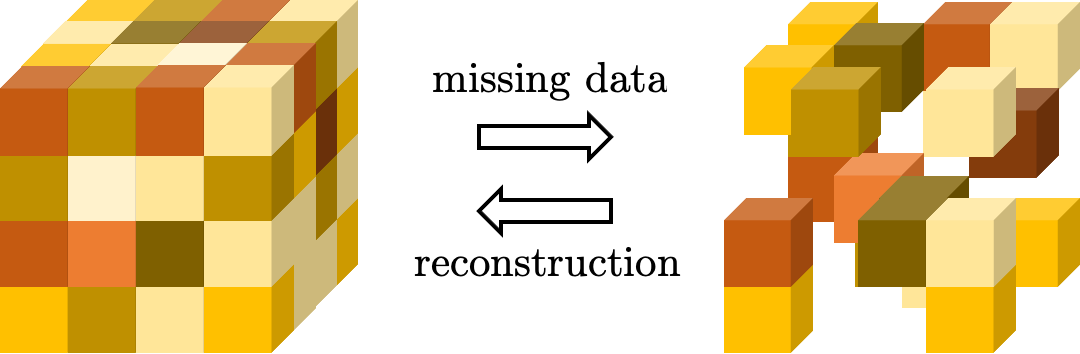
\includegraphics[width=0.65\textwidth]{figures/tensor_completion_plot.png}
\end{center}
\caption{Illustration of tensor completion, where we observe partial entries of an order-three tensor.\label{fig:tensor-completion-illustration}}
\end{figure}





\subsection{Problem formulation and assumptions}
\label{sec:setup-tensor-completion}


\paragraph{Notation.} Before describing our models, we introduce several notation that will be useful throughout. For any vectors $\bm{a}=[a_{i}]_{1\leq i\leq n},\bm{b}=[b_{i}]_{1\leq i\leq n},\bm{c}=[c_{i}]_{1\leq i\leq n}\in\mathbb{R}^{n}$,
the tensor $\bm{a}\otimes\bm{b}\otimes\bm{c}$ stands for an $n\times n\times n$
array whose $(i,j,k)$-th entry is given by $a_{i}b_{j}c_{k}$. Additionally, we denote by $\bm{a}\otimes \bm{b}\coloneqq  {\scriptsize \left[\begin{array}{c}
a_{1}\bm{b}\\
\vdots\\
a_{n}\bm{b}
\end{array}\right]}$ the Kronecker product between $\bm{a}$ and $\bm{b}$.  For any tensor $\bm{T}=[T_{i,j,k}]_{1\leq i,j,k\leq n}\in \mathbb{R}^{n\times n\times n}$, we say that $\bm{A}=[A_{i,j}]\in \mathbb{R}^{n\times n^2}$ is the mode-1 matricization of $\bm{T}$, denoted by $$\bm{A}=\mathsf{unfold}(\bm{T}),$$  if $A_{i,(j-1)n+k} = T_{i,j,k}$ for all $(i,j,k)\in [n]\times [n] \times [n]$.



\paragraph{Models and assumptions.}
Suppose the unknown order-three symmetric tensor $\bm{T}^{\star}=[T_{i,j,k}^{\star}]_{1\leq i,j,k\leq n}$  is a superposition of $r$ ($r<n$) rank-one symmetric tensors:
%
\begin{equation}
\bm{T}^{\star}=\sum_{i=1}^{r}\bm{w}_{i}^{\star}\otimes\bm{w}_{i}^{\star}\otimes\bm{w}_{i}^{\star} \in \mathbb{R}^{n\times n\times n},
\label{eq:defn-true-tensor}
\end{equation}
%
where $\{\bm{w}_i^{\star}\in \mathbb{R}^{n}\}$ represents a set of latent tensor factors.
What we have available are incomplete observations of the entries of  $\bm{T}^{\star}$. The observed data can be succinctly encoded by an index subset $\Omega \subseteq [n]\times [n] \times [n]$ (called a sampling set) and a tensor $\bm{T}=[T_{i,j,k}]_{1\leq i,j,k\leq n}$ as follows
%
\begin{equation}
T_{i,j,k}=\begin{cases}
T_{i,j,k}^{\star},\qquad & \text{if }(i,j,k)\in\Omega,\\
0, & \text{else}.
\end{cases}
\label{eq:observed-tensor-T}
\end{equation}
%
This subsection aims for an intermediate goal, namely, estimating the subspace spanned by $\{\bm{w}_i^{\star}\}_{1\leq i\leq r}$, which often serves as a crucial initial stage towards reliable completion of the whole tensor. The interested reader is referred to \citet{montanari2016spectral,cai2019tensorOR} for subsequent stages of tensor completion algorithms.


Similar to the matrix completion counterpart, we explore a {\em random sampling} pattern such that for all $(i,j,k)\in [n]\times [n] \times [n]$,
%
\begin{align}
	(i,j,k) \in \Omega \qquad \text{independently with probability }p.
\end{align}
%
In addition, we define for notational convenience that
%
\begin{equation}
	\nu_{i}\coloneqq\|\bm{w}_{i}^{\star}\|_{2}^{3},\qquad \nu_{\min}\coloneqq \min_{1\leq i\leq r}\nu_{i},\qquad \nu_{\max} \coloneqq \max_{1\leq i\leq r}\nu_{i},
	\label{eq:defn-wi-wmin-wmax-TC}
\end{equation}
%
where $\nu_{i}$ reflects the size of the rank-1 component $\bm{w}_{i}^{\star}\otimes \bm{w}_{i}^{\star}\otimes \bm{w}_{i}^{\star}$. The condition number of $\bm{T}^{\star}$ is then defined as $\kappa \coloneqq \nu_{\max} / \nu_{\min}$.

We shall also introduce several incoherence parameters as follows.
%
\begin{definition}
	Define the incoherence parameters of $\bm{T}^{\star}$ (cf.~\eqref{eq:defn-true-tensor}) as
	%
	\begin{equation}
		\mu_{1}\coloneqq\max_{1\leq i\leq r}\frac{n\|\bm{w}_{i}^{\star}\|_{\infty}^{2}}{\|\bm{w}_{i}^{\star}\|_{2}^{2}},
		\quad \text{and} \quad
		\mu_{2}\coloneqq\max_{i\neq j}\frac{n\big|\langle\bm{w}_{i}^{\star},\bm{w}_{j}^{\star}\rangle\big|^{2}}{\|\bm{w}_{i}^{\star}\|_{2}^{2} \, \|\bm{w}_{j}^{\star}\|_{2}^{2}} .
		\label{eq:defn-incoherence-TC}
	\end{equation}
	%
\end{definition}
%
Let us explain these parameters in words: small $\mu_1$ and $\mu_2$ reflect that (i) the energy of each tensor factor $\bm{w}_i^{\star}$ is spread out across different entries, and (ii) the factors $\{\bm{w}_i^{\star}\}$  are not too correlated with each other. To simplify presentation, we set
%
\begin{align*}
	\mu \coloneqq \max \{ \mu_1, \mu_2 \}.
\end{align*}


\subsection{Algorithm}
\label{sec:algorithm-TC}


Unfortunately, it is notoriously difficult to exploit the low-rank structure---and many other low-complexity structure---efficiently in the original tensor space \citep{hillar2013most}.
To circumvent this issue,
a natural strategy thus attempts to matricize the tensor data, followed by an application of suitable low-rank matrix estimation algorithms.   Specifically, let us unfold the tensor $\bm{T}^{\star}$ into an $n\times n^2$ matrix $\bm{A}^{\star}$ as follows
%
\begin{align}
	\bm{A}^{\star}\coloneqq \mathsf{unfold}\big( \bm{T}^{\star}\big)
	= \sum_{i=1}^{r}\bm{w}_{i}^{\star}\big(\bm{w}_{i}^{\star}\otimes\bm{w}_{i}^{\star}\big)^{\top} \in \mathbb{R}^{n\times n^2}.
	\label{eq:defn-Astar-TC}	
\end{align}
%
The resulting matrix $\bm{A}^{\star}$ inherits the low-rank structure, as it clearly has rank at most $r$. We shall also matricize the observed data as
%
\begin{align}
	\bm{A} \coloneqq \mathsf{unfold} ( \bm{T} ) .
	\label{eq:defn-A-TC}
\end{align}


In order to estimate the subspace $\bm{U}^{\star}$ spanned by $\{\bm{w}_i^{\star}\}_{1\leq i\leq r}$ (which is  the column space of $\bm{A}^{\star}$ as well), the spectral method studied here resorts to the rescaled Gram matrix $p^{-2} \bm{A} \bm{A}^{\top}$. As a sanity check, if there is absolutely no missing data (i.e., $p=1$), then $p^{-2} \bm{A} \bm{A}^{\top}$ reduces to $\bm{A}^{\star} \bm{A}^{\star\top}$, whose column space coincides with that of $\bm{A}^{\star}$.
Turning to the scenario with missing data, a close inspection reveals that
%
\begin{align}
	\frac{1}{p^{2}}\mathbb{E}\big[\bm{A}\bm{A}^{\top}\big]
	=  \bm{A}^{\star}\bm{A}^{\star\top}+ \Big(\frac{1}{p}-1\Big) \mathcal{P}_{\mathsf{diag}} \big(\bm{A}^{\star}\bm{A}^{\star\top}\big),
	\label{eq:expectation-gram-matrix-TC}
\end{align}
%
where $\mathcal{P}_{\mathsf{diag}} (\cdot)$ denotes the Euclidean projection onto the set of matrices with zero off-diagonal entries.
This, however, makes apparent a severe issue: in the highly subsampled regime (i.e., where $p$ is small), the diagonal components might be excessively large and non-identical, thus destroying the low-rank structure in  \eqref{eq:expectation-gram-matrix-TC}.


To mitigate their undesirable effects, it is advisable to properly adjust the sizes of the diagonal entries \citep{montanari2016spectral,cai2019subspace}.
As it turns out, a simple yet plausible scheme is {\em diagonal deletion}, which exploits only the off-diagonal part as follows
\begin{subequations}
%
\begin{align}
	\bm{M} \coloneqq \frac{1}{p^{2}} \mathcal{P}_{\mathsf{off}\text{-}\mathsf{diag}}\big(\bm{A}\bm{A}^{\top}\big) .
	%\underset{\text{an off-diagonal matrix}}{\underbrace{\frac{1}{p^{2}}\Big(\bm{A}\bm{A}^{\top}-\mathcal{P}_{\mathsf{diag}}\big(\bm{A}\bm{A}^{\top}\big)\Big)}} .
	% + \underset{\text{a diagonal matrix}}{\underbrace{\frac{1}{p}\mathcal{P}_{\mathsf{diag}}\big(\bm{A}\bm{A}^{\top}\big)}}.	
	\label{defn:gram-matrix-TC}
\end{align}
%
Here,  $\mathcal{P}_{\mathsf{off}\text{-}\mathsf{diag}}(\cdot)$ stands for the operator that zeros out all diagonal entries of a matrix.
%which zeros out all diagonal entries.
% In words, we zero out the diagonal part of $\bm{A}\bm{A}^{\top}$ so as to mitigate its negative influence.
% the off-diagonal part and the diagonal part of $\bm{A}\bm{A}^{\top}$ are rescaled with different scaling factors. This careful scaling scheme ensures that unbiasedness of $\bm{M}$ in the sense that
%
One can easily verify that, in expectation,
%
\begin{equation}
	\mathbb{E}[\bm{M}]=   \underset{\eqqcolon\, \bm{M}^{\star} }{\underbrace{  \bm{A}^{\star}\bm{A}^{\star\top} }} - \mathcal{P}_{\mathsf{diag}}\big( \bm{A}^{\star}\bm{A}^{\star\top} \big),
	\label{eq:defn-Mstar-TC}
\end{equation}
%
\end{subequations}
which stays quite close to the low-rank matrix $\bm{M}^{\star}$ as long as the diagonal entries of $\bm{M}^{\star}$ are small enough.
The spectral method then proceeds by calculating the top-$r$ eigendecomposition $\bm{U}\bm{\Lambda}\bm{U}^{\top}$ of $\bm{M}$ and returning $\bm{U}$ as the subspace estimate. Here, the columns of $\bm{U}\in \mathbb{R}^{n\times r}$ are formed by the $r$ leading eigenvectors of $\bm{M}$, while $\bm{\Lambda}\in \mathbb{R}^{r\times r}$ is a diagonal matrix containing the $r$ leading eigenvalues.


\begin{remark}
	The diagonal deletion idea has been recommended not just for tensor completion, but also for problems including but not limited to bi-clustering \citep{florescu2016spectral}, PCA with missing data and/or heteroskedastic noise  \citep{cai2019subspace,abbe2020ell_p}, and contextual community detection \citep{abbe2020ell_p}.  Instead of diagonal deletion, one might also consider properly rescaling the diagonal entries
	based on the sampling mechanism; see, e.g., \citet{montanari2016spectral,lounici2014high,loh2012high,zhang2018heteroskedastic,zhu2019high}. 
\end{remark}









\subsection{Performance guarantees}
\label{sec:theory-TC}


The aforementioned spectral method can be analyzed by means of the $\ell_{2}$ perturbation theory as well.
As usual, this requires first
controlling the size of $\bm{E} \coloneqq \bm{M}-\bm{M}^{\star}$, where $\bm{M}$ and $\bm{M}^{\star}$ are defined in \eqref{defn:gram-matrix-TC} and \eqref{eq:defn-Mstar-TC}, respectively.
%
\begin{lemma}
	\label{lem:size-E-TC}
	Consider the settings in Section~\ref{sec:setup-tensor-completion}. There exists some universal constant $C>0$ such that with probability at least $1-O(n^{-7})$,
	%
	\begin{align}
		\|\bm{E}\| \leq C  \Bigg( \frac{\mu^{3/2}r\sqrt{\log n}}{n^{3/2}p} + \sqrt{\frac{\mu^{2}r\log n}{n^{2}p}}  + \frac{\mu r}{n} \Bigg)\nu_{\max}^{2},
	\end{align}
	%
	provided that $p\gtrsim \frac{\mu^{3/2}r\log^{2.5}n}{n^{3/2}}$ and that $\mu \max\{\log n, r^2\kappa^4 \} \leq c_3 n$ for some sufficiently small constant $c_3>0$.
\end{lemma}
%


In order to apply the Davis-Kahan $\sin\bm{\Theta}$ theorem (cf.~Corollary~\ref{cor:davis-kahan-conclusion-corollary}), another step boils down to characterizing the eigengap of the matrix $\bm{M}^{\star}=\bm{A}^{\star}\bm{A}^{\star\top}$ of interest. Our result is this:
%
\begin{lemma}
	\label{lemma:spectrum-Astar-AstarT-TC}
	Suppose that $\mu r^{2}\kappa^{4}\leq c_{3}n$ for some sufficiently small constant $c_3>0$. Then the $i$-th largest eigenvalue of $\bm{A}^{\star}\bm{A}^{\star\top}$ obeys
	%
	\begin{align*}
		\lambda_{i}\big(\bm{A}^{\star}\bm{A}^{\star\top}\big) & \in\ \big[\nu_{\min}^{2}/2, 2\nu_{\max}^2 \big], \qquad \text{if }1\leq i\leq r; \\
		\lambda_{i}\big(\bm{A}^{\star}\bm{A}^{\star\top}\big) & =0,\qquad\qquad\qquad\qquad ~\text{if }i\geq r+1.
	\end{align*}
	%
\end{lemma}
%
The preceding two lemmas, which will be established in Section~\ref{sec:proof-auxiliary-lemmas-TC}, readily lead to the following statistical guarantees for the spectral method presented in Section~\ref{sec:algorithm-TC}.
%
\begin{theorem}
	\label{thm:performance-TC-l2}
	Consider the settings in Section~\ref{sec:setup-tensor-completion}. Suppose that
	%
	\begin{align}
			\mu r^{2}\kappa^{4}\log n \leq c_4 n
			\qquad \text{and} \qquad
			p\geq c_{5} \frac{\mu^{3/2}\kappa^{2}r \log^{2.5} n} {n^{3/2}}
			% \max \Bigg\{
			%,\frac{\mu^{2}\kappa^{4}r\log n}{n^{2}}\Bigg\}
			\label{eq:condition-TC}
	\end{align}
	%
	hold for some small (resp.~large) enough constant $c_4>0$ (resp.~$c_5>0$). Then with probability at least $1-O(n^{-7})$, one has
	%
	\[
		\mathsf{dist}\big(\bm{U},\bm{U}^{\star}\big)
		\lesssim \frac{\mu^{3/2}\kappa^{2}r\sqrt{\log n}}{n^{3/2}p}+\sqrt{\frac{\mu^{2}\kappa^{4}r\log n}{n^{2}p}}+\frac{\mu\kappa^{2}r}{n} .
	\]
	%
\end{theorem}
%
\begin{proof}
In view of Lemmas~\ref{lem:size-E-TC}-\ref{lemma:spectrum-Astar-AstarT-TC}, one would have $\|\bm{E}\|\leq (1-1/\sqrt{2}) \lambda_{r} (\bm{M}^{\star} )$ under Condition \eqref{eq:condition-TC}.
%
%\[
%	\mu r\kappa^{2}\leq c_4n, \quad
%	p\geq c_{5}\max\Bigg\{\frac{\mu^{3/2}\kappa^{2}r\sqrt{\log n}}{n^{3/2}},\frac{\mu^{2}\kappa^{4}r\log n}{n^{2}}\Bigg\}
%\]
%
%hold for some small (resp.~large) enough constant $c_4>0$ (resp.~$c_5>0$).
%
Corollary~\ref{cor:davis-kahan-conclusion-corollary} combined with Lemma~\ref{lem:size-E-TC} then tells us that, with probability at least $1-O(n^{-7})$,
%
\[
	\mathsf{dist}\big(\bm{U},\bm{U}^{\star}\big)
	\leq \frac{2\big\|\bm{E}\big\|}{\lambda_{r}(\bm{M}^{\star})}\lesssim\frac{\Big(\frac{\mu^{3/2}r\sqrt{\log n}}{n^{3/2}p}+\sqrt{\frac{\mu^{2}r\log n}{n^{2}p}}+\frac{\mu r}{n}\Big)\nu_{\max}^{2}}{\nu_{\min}^{2}}
\]
%
as desired. \end{proof}



Theorem~\ref{thm:performance-TC-l2} is noteworthy for its implication on the sample complexity. To be precise, consider, for simplicity, the scenario where $r,\mu,\kappa = O(1)$.
In order to achieve consistent estimation in the sense that $\mathsf{dist}\big(\bm{U},\bm{U}^{\star}\big)=o(1)$, it suffices for the sample size---which sharply concentrates around $n^3p$ under our model---to exceed
%
\[
	n^{3}p\gtrsim n^{3/2}\mathrm{poly}\log(n).
\]
%


The careful reader might immediately remark that this sample complexity remains substantially higher than the information-theoretic limit,
the latter of which is $nr=O(n)$ in this case since there are only $nr$ free parameters. It is worth noting, however, that all polynomial-time algorithms developed in the literature for tensor completion require a sample size at least exceeding the order of $n^{3/2}$ \citep{barak2016noisy}. This hints at the (potential) existence of a computational barrier that prevents one from achieving the information-theoretic limit efficiently. Viewed in this light, the spectral method presented herein already achieves near-optimal sample complexity---when restricted to  computationally tractable algorithms---if the objective is consistent subspace estimation.






\subsection{Proof of auxiliary lemmas}
\label{sec:proof-auxiliary-lemmas-TC}




\paragraph{Proof of Lemma~\ref{lem:size-E-TC}.}
Define the following zero-mean random matrix
%
\[
	\bm{Z}=p^{-1}\bm{A}-\bm{A}^{\star}.
\]
%
It is  self-evident that
%
\[
  p^{-2} \big(\bm{A}\bm{A}^{\top}-\mathbb{E}\big[\bm{A}\bm{A}^{\top}\big]\big)=\bm{A}^{\star}\bm{Z}^{\top}+\bm{Z}\bm{A}^{\star\top}
+ \big( \bm{Z}\bm{Z}^{\top}-\mathbb{E}\big[\bm{Z}\bm{Z}^{\top}\big] \big),
\]
%
which implies that the identity holds for the off-diagonal part.  By the definitions
\eqref{defn:gram-matrix-TC} and \eqref{eq:defn-Mstar-TC}, it follows from the triangle inequality that
%
\begin{align}
\big\|\bm{M}-\bm{M}^{\star}\big\| & \leq\big\|\mathcal{P}_{\mathsf{diag}}\big(\bm{A}^{\star}\bm{A}^{\star\top}\big)\big\|+2\big\|\mathcal{P}_{\mathsf{off}\text{-}\mathsf{diag}}\big(\bm{A}^{\star}\bm{Z}^{\top}\big)\big\|\nonumber \\
	& \qquad+\big\|\mathcal{P}_{\mathsf{off}\text{-}\mathsf{diag}}\big(\bm{Z}\bm{Z}^{\top} -\mathbb{E}\big[\bm{Z}\bm{Z}^{\top} \big] \big)\big\|.
	\label{eq:decompose-M-Mstar-Z-Astar-TC}
\end{align}
%
In the sequel, we shall discuss how to control the three terms on the right-hand side of \eqref{eq:decompose-M-Mstar-Z-Astar-TC} separately.


\bigskip\noindent
{\em Step 1: bounding $\|\mathcal{P}_{\mathsf{diag}} (\bm{A}^{\star}\bm{A}^{\star\top})\|$.}
It is straightforward to verify that
%the term $\mathcal{P}_{\mathsf{diag}} (\bm{A}^{\star}\bm{A}^{\star\top}),$
% whose spectral norm obeys
%
\begin{equation}
\big\|\mathcal{P}_{\mathsf{diag}}\big(\bm{A}^{\star}\bm{A}^{\star\top}\big)\big\|=\max_{1\leq l\leq n}\big\|\bm{A}_{l,\cdot}^{\star}\big\|_{2}^{2}=\big\|\bm{A}^{\star}\big\|_{2,\infty}^{2}.
	\label{eq:P-diag-AAT-bound-TC}
\end{equation}
%
It thus suffices to  bound $\|\bm{A}^{\star}\|_{2,\infty}$, which we shall discuss momentarily.


%Regarding $\|\bm{A}^{\star}\bm{Z}^{\top}\|$, let us write
%%
%\[
%\bm{A}^{\star}\bm{Z}^{\top}=\sum_{i=1}^{n^{2}}\bm{A}_{\cdot,i}^{\star}\big(\bm{Z}_{\cdot,i}\big)^{\top},
%\]
%%
%which is a sum of independent rank-1 matrices and can be controlled via the matrix Bernstein inequality. Towards this,
%


\bigskip\noindent
{\em Step 2: bounding $\|\mathcal{P}_{\mathsf{off}\text{-}\mathsf{diag}} (\bm{Z}\bm{Z}^{\top} -\mathbb{E}[\bm{Z}\bm{Z}^{\top} ] ) \|$.}
 Define a collection of independent {\em zero-mean} random matrices as follows
%
\[
	\bm{Q}_{i}\coloneqq  \mathcal{P}_{\mathsf{off}\text{-}\mathsf{diag}}\big(\bm{Z}_{\cdot,i}\bm{Z}_{\cdot,i}^{\top}\big),
	\qquad 1\leq i\leq n^2,
\]
%
with which we can express
%
\begin{align}
	\mathcal{P}_{\mathsf{off}\text{-}\mathsf{diag}}\big(\bm{Z}\bm{Z}^{\top} -\mathbb{E}\big[\bm{Z}\bm{Z}^{\top}\big] \big)
	= \sum\nolimits_i  \Big( \bm{Q}_{i} - \mathbb{E}\big[ \bm{Q}_{i} \big] \Big) = \sum\nolimits_i  \bm{Q}_{i} .
	\label{eq:P-offdiag-ZZ-TC}
\end{align}
%
Here the last relation uses the fact that $\mathcal{P}_{\mathsf{off}\text{-}\mathsf{diag}} (\mathbb{E}[\bm{Z}\bm{Z}^{\top} ] ) = \sum_{i}\mathbb{E}\big[ \bm{Q}_{i} \big] = \bm{0}$.
Recognizing that the entries of $\bm{Z}_{\cdot,i}$ are independently
generated, one can see from straightforward calculations that $\mathbb{E}\big[\bm{Q}_{i}\bm{Q}_{i}^{\top}\big]$
is a diagonal matrix, whose diagonal entries satisfy
%
\begin{align*}
\Big(\mathbb{E}\big[\bm{Q}_{i}\bm{Q}_{i}^{\top}\big]\Big)_{l,l} & =\mathbb{E}\big[Z_{l,i}^{2}\big]\sum_{j:j\neq l}\mathbb{E}\big[Z_{j,i}^{2}\big]
  = \frac{1-p}{p}\big(A_{l,i}^{\star}\big)^{2}\sum_{j:j\neq l}\frac{1-p}{p}\big(A_{j,i}^{\star}\big)^{2}\\
 & \leq\frac{1}{p^{2}}\big(A_{l,i}^{\star}\big)^{2}\big\|\bm{A}_{\cdot,i}^{\star}\big\|_{2}^{2}
	\leq\frac{1}{p^{2}}\big(A_{l,i}^{\star}\big)^{2}\big\|\bm{A}^{\star}\big\|_{\infty,2}^{2}
\end{align*}
%
for all $1\leq l\leq n$.  Taking into account all samples yields
%
\[
	\sum_{i=1}^{n^2}\Big(\mathbb{E}\big[\bm{Q}_{i}\bm{Q}_{i}^{\top}\big]\Big)_{l,l}\leq\frac{1}{p^{2}}\sum_{i=1}^{n^{2}}\big(A_{l,i}^{\star}\big)^{2}\big\|\bm{A}^{\star}\big\|_{\infty,2}^{2}\leq\frac{1}{p^{2}}\big\|\bm{A}^{\star}\big\|_{2,\infty}^{2}\big\|\bm{A}^{\star}\big\|_{\infty,2}^{2}
\]
%
for any $1\leq l\leq n$,  which together with the diagonal structure of $\mathbb{E}\big[\bm{Q}_{i}\bm{Q}_{i}^{\top}\big]$ leads to an upper bound on the variance statistic
%
\begin{align*}
	v  \coloneqq\Big\|\sum_{i}\mathbb{E}\big[\bm{Q}_{i}\bm{Q}_{i}^{\top}\big]\Big\|
	= \Big|\max_{l}\Big(\sum_{i}\Big(\mathbb{E}\big[\bm{Q}_{i}\bm{Q}_{i}^{\top}\big]\Big)_{l,l}\Big)\Big|
	\leq\frac{  \big\|\bm{A}^{\star}\big\|_{2,\infty}^{2}\big\|\bm{A}^{\star}\big\|_{\infty,2}^{2} }{p^{2}}.
\end{align*}
%
In addition, we identify a suitable truncation level and claim that
%
\begin{subequations}
	\label{eq:Qi-tail-bound-exp-bound-TC}
\begin{align}
\mathbb{P}\Big\{\big\|\bm{Q}_{i}\big\|_{2}\geq L\Big\} & \leq2n^{-7}\eqqcolon q_{0},\\
\Big\|\mathbb{E}\big[\bm{Q}_{i}\mathbbm1\big\{\big\|\bm{Q}_{i}\big\|_{2}\leq L\big\}\big]\Big\| & \leq4n^{-7}p^{-2}\big\|\bm{A}^{\star}\big\|_{\infty,2}^{2}\eqqcolon q_{1},	
\end{align}
\end{subequations}
%
where we define $L \coloneqq 2\big(4\sqrt{\frac{\log n}{p}}\big\|\bm{A}^{\star}\big\|_{\infty,2}+\frac{6\log n}{p}\big\|\bm{A}^{\star}\big\|_{\infty}\big)^2$.
Armed with these observations, the truncated matrix Bernstein inequality (see Corollary~\ref{thm:matrix-Bernstein-friendly-truncated}) taken together with \eqref{eq:P-offdiag-ZZ-TC} reveals that
%
\begin{align}
 & \big\|\mathcal{P}_{\mathsf{off}\text{-}\mathsf{diag}}\big(\bm{Z}\bm{Z}^{\top}-\mathbb{E}\big[\bm{Z}\bm{Z}^{\top}\big]\big)\big\|
   \lesssim\sqrt{v\log n}+L\log n+n^{2}q_{1} \notag\\
 &  \lesssim\frac{\sqrt{\log n}}{p}\big\|\bm{A}^{\star}\big\|_{2,\infty}\big\|\bm{A}^{\star}\big\|_{\infty,2}+ \frac{\log^{2}n}{p} \big\|\bm{A}^{\star}\big\|_{\infty,2}^{2}+\frac{\log^{3}n}{p^{2}}\big\|\bm{A}^{\star}\big\|_{\infty}^{2}
	\label{eq:P-off-diag-ZZt-intermediate-TC}
\end{align}
%
with probability  $1- O(n^{-7}) - nq_0=1- O(n^{-7})$, provided that $p\gtrsim n^{-5}$.





\bigskip\noindent
{\em Step 3: bounding $\|\mathcal{P}_{\mathsf{off}\text{-}\mathsf{diag}}(\bm{A}^{\star}\bm{Z}^{\top})\|$.} This term can be controlled in a similar fashion as $\|\mathcal{P}_{\mathsf{off}\text{-}\mathsf{diag}} (\bm{Z}\bm{Z}^{\top} -\mathbb{E}[\bm{Z}\bm{Z}^{\top} ] ) \|$.  We thus omit the details and only state the result as follows:
%
\begin{align}
	& \|\mathcal{P}_{\mathsf{off}\text{-}\mathsf{diag}}(\bm{A}^{\star}\bm{Z}^{\top})\|
	\lesssim
	\big\|\bm{A}^{\star}\big\|_{\infty,2}\big\|\bm{A}^{\star}\big\|\sqrt{\frac{\log n}{p}} \notag\\
	& \qquad
	+\sqrt{\frac{\log^{3}n}{p}}\big\|\bm{A}^{\star}\big\|_{\infty,2}^{2} + \|\bm{A}^{\star}\|_{\infty,2}\big\|\bm{A}^{\star}\big\|_{\infty}\frac{\log^{2}n}{p}
	\label{eq:P-offdiag-AZ-intermediate-TC}
\end{align}
%
holds with probability at least $1-O(n^{-7})$.



\bigskip\noindent
{\em Step 4:}
To finish up,  we are in need of bounding $\|\bm{A}^{\star}\|_{\infty,2}$, $\|\bm{A}^{\star}\|_{2,\infty}$ and $\|\bm{A}^{\star}\|_{\infty}$, which is accomplished in the following lemma.
%
\begin{lemma}
	\label{lem:size-W-Wlift-TC}
	Suppose that $\mu r^{2}\leq n$. Then one has
	%
\begin{align*}
%	\big\|\bm{W}^{\star}\big\|&\leq\sqrt{2}v_{\max}^{1/3},\qquad\qquad  &\big\|\bm{W}^{\star}\big\|_{2,\infty} &\leq\sqrt{\frac{\mu r}{n}}v_{\max}^{1/3},  \\
	 \big\|\bm{A}^{\star}\big\|_{\infty} \leq\frac{\mu^{3/2}r\nu_{\max}}{n^{3/2}}  , ~~
	\big\|\bm{A}^{\star}\big\|_{\infty,2} \leq \frac{\mu \sqrt{2r}\nu_{\max}}{n} ,
	~~ \big\|\bm{A}^{\star}\big\|_{2,\infty}  \leq\sqrt{\frac{2\mu r}{n}}\nu_{\max} .
\end{align*}
%
\end{lemma}
%
Taking Lemma \ref{lem:size-W-Wlift-TC} collectively with \eqref{eq:P-diag-AAT-bound-TC}, \eqref{eq:P-off-diag-ZZt-intermediate-TC}, \eqref{eq:P-offdiag-AZ-intermediate-TC} and combining terms, we arrive at
%
\begin{align*}
\eqref{eq:P-diag-AAT-bound-TC} + \eqref{eq:P-off-diag-ZZt-intermediate-TC} + \eqref{eq:P-offdiag-AZ-intermediate-TC}
% & \lesssim\Bigg(\frac{\mu^{5/2}r^{3/2}\sqrt{\log n}}{n^{5/2}p}+\frac{\mu^{2}r\log^{2}n}{n^{2}p}+\frac{\mu^{3}r^{2}\log^{3}n}{n^{3}p^{2}}\Bigg)\nu_{\max}^{2}\\
	& \lesssim\Bigg(
	%\frac{\mu^{3}r^{2}\log^{3}n}{n^{3}p^{2}} +\frac{\mu^{2}r\log^{2}n}{n^{2}p}
	\frac{\mu^{3/2}r\sqrt{\log n}}{n^{3/2}p} + \sqrt{\frac{\mu^{2}r\log n}{n^{2}p}}  + \frac{\mu r}{n} \Bigg)\nu_{\max}^{2}
\end{align*}
%
with probability at least $1-O(n^{-7})$,
provided that $\mu \log n \leq n$ and $p\gtrsim \frac{\mu^{3/2}r\log^{2.5}n}{n^{3/2}}$. This taken together with \eqref{eq:decompose-M-Mstar-Z-Astar-TC} concludes the proof.






%Next, we remark that the second and the third terms on the right-hand side of \eqref{eq:decompose-M-Mstar-Z-Astar-TC} can be controlled via similar arguments. Here, we shall focus primarily on bounding  $\|\mathcal{P}_{\mathsf{off}\text{-}\mathsf{diag}} (\bm{Z}\bm{Z}^{\top} -\mathbb{E}[\bm{Z}\bm{Z}^{\top} ] ) \|$.


\bigskip\noindent
{\em Proof of the relation~\eqref{eq:Qi-tail-bound-exp-bound-TC}.}
%
We first make note of a connection between $\bm{Q}_{i}$ and $\bm{Z}_{\cdot,i}$ as follows
%
\begin{equation}
	\big\|\bm{Q}_{i}\big\|\leq\big\|\bm{Z}_{\cdot,i}\bm{Z}_{\cdot,i}^{\top}\big\|+\big\|\mathcal{P}_{\mathsf{diag}}\big(\bm{Z}_{\cdot,i}\bm{Z}_{\cdot,i}^{\top}\big)\big\|\leq2\big\|\bm{Z}_{\cdot,i}\big\|_{2}^{2},
	\label{eq:Qi-Zi-relation-TC}
\end{equation}
%
which motivates us to first control the size of $\bm{Z}_{\cdot,i}$.
By construction, each entry $Z_{j,i}$ can be written as $Z_{j,i}= \big(\frac{1}{p} \delta_{j,i} -1\big) A_{j,i}^{\star}$, where $\{\delta_{j,i}\}$ is a collection of independent Bernoulli random variables with mean $p$. This observation allows one to derive  % invoke Lemma~\ref{lem:size-W-Wlift-TC} to
%
\begin{align*}
B_{z} & \coloneqq\max_{i,j}\big|Z_{j,i}\big|\leq \frac{1}{p} \big\|\bm{A}^{\star}\big\|_{\infty} ;\\
	%\leq\frac{\mu^{3/2}r}{pn^{3/2}}\nu_{\max};\\
v_{z} & \coloneqq\mathbb{E}\Big[\big\|\bm{Z}_{\cdot,i}\big\|_{2}^{2}\Big] = \frac{1-p}{p}\sum\nolimits_{j}\big(A_{j,i}^{\star}\big)^{2} \leq\frac{1}{p}\big\|\bm{A}^{\star}\big\|_{\infty,2}^{2} .
	%\leq\frac{2\mu^{2}r}{pn^{2}}\nu_{\max}^{2}.
\end{align*}
%
The matrix Bernstein inequality (see Corollary~\ref{thm:matrix-Bernstein-friendly})  then yields
%
\begin{align}
%\big\|\bm{Z}_{\cdot,i}\big\|_{2} & \leq4\sqrt{v_{z}\log n}+6B_{z}\log n \nonumber\\
% & \leq\Bigg(4\sqrt{\frac{2\mu^{2}r\log n}{pn^{2}}}+\frac{6\mu^{3/2}r\log n}{pn^{3/2}}\Bigg)\nu_{\max}
%	\eqqcolon\beta_{z}
\big\|\bm{Z}_{\cdot,i}\big\|_{2} & \leq4\sqrt{v_{z}\log n}+6B_{z}\log n\nonumber\\
 & \leq \Bigg(4\sqrt{\frac{\log n}{p}}\big\|\bm{A}^{\star}\big\|_{\infty,2}+\frac{6\log n}{p}\big\|\bm{A}^{\star}\big\|_{\infty}\Bigg) \eqqcolon\beta_{z}
\label{eq:Zi-UB-betaz-TC}
\end{align}
%
with probability at least $1-2n^{-7}$, which combined with \eqref{eq:Qi-Zi-relation-TC} gives
%
\begin{align}
	\mathbb{P}\Big\{ \big\|\bm{Q}_{i}\big\|_{2}  \geq 2\beta_{z}^2 \Big\} \leq 2n^{-7}.
\label{eq:Qi-Zi-UB-betaz-TC}
\end{align}
%
Recalling that $\mathbb{E}[\bm{Q}_i]=\bm{0}$, one can derive
%
\begin{align*}
 & \Big\|\mathbb{E}\big[\bm{Q}_{i}\mathbbm1\big\{\big\|\bm{Q}_{i}\big\|_{2}\leq2\beta_{z}^{2}\big\}\big]\Big\|=\Big\|\mathbb{E}\big[\bm{Q}_{i}\big]-\mathbb{E}\big[\bm{Q}_{i}\mathbbm1\big\{\big\|\bm{Q}_{i}\big\|_{2}>2\beta_{z}^{2}\big\}\big]\Big\|\\
	& \quad=\Big\|\mathbb{E}\big[\bm{Q}_{i}\mathbbm1\big\{\big\|\bm{Q}_{i}\big\|_{2}>2\beta_{z}^{2}\big\}\big]\Big\|\overset{(\mathrm{i})}{\leq}\mathbb{P}\big\{\big\|\bm{Q}_{i}\big\|_{2}>2\beta_{z}^2 \big\}\cdot  \frac{2}{p^{2}}\big\|\bm{A}^{\star}_{\cdot,i}\big\|_{2}^{2} \\
 & \quad\overset{(\mathrm{ii})}{\leq}  \frac{4}{n^7p^{2}}\big\|\bm{A}^{\star}\big\|_{\infty,2}^{2} .
	%\overset{(\mathrm{iii})}{\leq}\frac{4\mu^{2}r}{n^{9}p^{2}}\nu_{\max}^{2}\overset{(\mathrm{iv})}{\leq}\frac{1}{n^{8}p^2}\nu_{\max}^{2}.
\end{align*}
%
Here, (i) relies on \eqref{eq:Qi-Zi-relation-TC} and the fact $\|\bm{Z}_{\cdot,i}\|_2\leq p^{-1}\|\bm{A}^{\star}_{\cdot,i}\|_2$ (by construction), whereas (ii) results from the calculation in \eqref{eq:Zi-UB-betaz-TC}.
% (iii) is a consequence of Lemma~\ref{lem:size-W-Wlift-TC}, whereas (iv) holds provided that $4\mu^2 r \leq n$.







\paragraph{Proof of Lemma~\ref{lemma:spectrum-Astar-AstarT-TC}.}
%
Define the normalized tensor factors as 
%
\[
	\overline{\bm{w}}_{i}^{\star}:=\bm{w}_{i}^{\star}/\left\Vert \bm{w}_{i}^{\star}\right\Vert _{2}
	\qquad (1\leq i\leq r),
\]
%
and it is convenient to introduce the following auxiliary matrices that contain information about them:
%
\begin{align*}
\overline{\bm{W}}^{\star}\coloneqq \left[\overline{\bm{w}}_{1}^{\star},\cdots,\overline{\bm{w}}_{r}^{\star}\right],\qquad\overline{\bm{W}}_{\mathsf{lift}}^{\star}\coloneqq \left[\overline{\bm{w}}_{1}^{\star}\otimes\overline{\bm{w}}_{1}^{\star},\cdots,\overline{\bm{w}}_{r}^{\star}\otimes\overline{\bm{w}}_{r}^{\star}\right].
\end{align*}
%
Additionally, we introduce a diagonal matrix $\bm{D}^{\star}\in\mathbb{R}^{r\times r}$ whose diagonal entries are given by
%
\[
	\big[ \bm{D}^{\star} \big]_{i,i} =\big\| \bm{w}_{i}^{\star} \big\|_{2}^3 = v_{i},\qquad1\leq i\leq r.
\]
%
The matrices introduced above allow one to express $\bm{A}^{\star} =\overline{\bm{W}}^{\star} \bm{D}^{\star}  \overline{\bm{W}}^{\star\top}_{\mathsf{lift}} $ and $\bm{A}^{\star}\bm{A}^{\star\top}$ as follows
%
\begin{align}
	\label{defn:Astar-Astar-top-expression-TC}
%\bm{G}^{\star}=
	\bm{A}^{\star}\bm{A}^{\star\top}=\overline{\bm{W}}^{\star} \bm{D}^{\star}  \overline{\bm{W}}^{\star\top}_{\mathsf{lift}} \overline{\bm{W}}^{\star}_{\mathsf{lift}}   \bm{D}^{\star}   \overline{\bm{W}}^{\star\top}.
\end{align}
%
Clearly, the rank of $\bm{A}^{\star}\bm{A}^{\star\top}$ is bounded above by $r$, and hence it suffices to lower bound $\lambda_i(\bm{A}^{\star}\bm{A}^{\star\top})$ when $i\leq r$.


In order to characterize the spectrum of $\bm{A}^{\star}\bm{A}^{\star\top}$, we  first look at the eigenvalues of $\overline{\bm{W}}^{\star\top} \overline{\bm{W}}^{\star}$ and $\overline{\bm{W}}^{\star\top}_{\mathsf{lift}} \overline{\bm{W}}^{\star}_{\mathsf{lift}}$. Write
%
\begin{equation}
	\overline{\bm{W}}^{\star\top} \overline{\bm{W}}^{\star}=\bm{I}_{r}+ \bm{R}, 
	\qquad\text{and}\qquad
	\overline{\bm{W}}^{\star\top}_{\mathsf{lift}}\overline{\bm{W}}^{\star}_{\mathsf{lift}}
	=\bm{I}_{r}+{\bm{R}}_{\mathsf{lift}}
	\label{eq:W_top_residual_decomp}
\end{equation}
%
for some residual matrices $\bm{R},{\bm{R}}_{\mathsf{lift}}\in\mathbb{R}^{r\times r}$ (which are off-diagonal matrices). By virtue of the definition \eqref{eq:defn-incoherence-TC}, we immediately obtain
%
\begin{equation*}
	\left\Vert \bm{R}\right\Vert _{\infty}\leq\sqrt{\mu /n},
	\qquad\text{and}\qquad
	\big\|{\bm{R}}_{\mathsf{lift}}\big\|_{\infty}\leq\mu /n,
\end{equation*}
%
thus indicating that
%
\begin{equation}
	\| \bm{R}\| \leq r\left\Vert \bm{R}\right\Vert _{\infty}\leq r\sqrt{\mu /n},
	%\quad \text{and} \quad
	\quad ~~
	\big\|{\bm{R}}_{\mathsf{lift}} \big\|\leq r \, \big\|{\bm{R}}_{\mathsf{lift}}\big\|_{\infty}\leq\mu r /  n .
	\label{eq:spectral-norm-residual_C_UB}
\end{equation}
%
Putting these together with \eqref{eq:W_top_residual_decomp} and invoking Weyl's inequality give
\begin{align}
\label{eq:spectraum-WWstar-bar-TC}
\max_{i}\Big|\lambda_{i}\big(\overline{\bm{W}}^{\star\top}\overline{\bm{W}}^{\star}\big)-1\Big| & \leq\left\Vert \bm{R}\right\Vert \leq r\sqrt{\mu /n},
% \\
%\max_{i}\Big|\lambda_{i}\big(\overline{\bm{W}}_{\mathsf{lift}}^{\star\top}\overline{\bm{W}}_{\mathsf{lift}}^{\star}\big)-1\Big| & \leq\big\|\bm{R}_{\mathsf{lift}}\big\|\leq\mu_{2}r/n,
\end{align}
%
which together with the assumption $\mu r^{2}\leq n$ further reveals that
%
\begin{align}
\label{eq:W_op_UB}
\big\|\overline{\bm{W}}^{\star}\big\| & =\sqrt{\lambda_{1}\big(\overline{\bm{W}}^{\star\top}\overline{\bm{W}}^{\star}\big)}\leq\sqrt{1+r\sqrt{\mu /n}} \leq 2.
%\big\|\overline{\bm{W}}_{\mathsf{lift}}^{\star}\big\| & =\sqrt{\lambda_{1}\big(\overline{\bm{W}}_{\mathsf{lift}}^{\star\top}\overline{\bm{W}}_{\mathsf{lift}}^{\star}\big)}\leq\sqrt{1+\mu_{2}r/n} \leq 2.
\end{align}
%






We now return to study $\bm{A}^{\star}\bm{A}^{\star\top}$. In view of \eqref{defn:Astar-Astar-top-expression-TC} and \eqref{eq:W_top_residual_decomp}, one can decompose $\bm{A}^{\star}\bm{A}^{\star\top}$ into the following two terms
%
\begin{align}
	\bm{A}^{\star}\bm{A}^{\star\top}
	=  \underset{\eqqcolon\, \bm{G}_1 }{\underbrace{  \overline{\bm{W}}^{\star} \big( \bm{D}^{\star} \big)^2 \overline{\bm{W}}^{\star\top} }}
	+  \underset{\eqqcolon\, \bm{G}_2 }{\underbrace{ \overline{\bm{W}}^{\star}  \bm{D}^{\star}  {\bm{R}_{\mathsf{lift}}}  \bm{D}^{\star}   \overline{\bm{W}}^{\star\top} }}.
	\label{eq:decomposition-AAstar-G1-G2-TC}
\end{align}
%
Making use of the bounds \eqref{eq:spectral-norm-residual_C_UB} and \eqref{eq:W_op_UB} immediately leads to
%
\[
	\big\|\bm{G}_{2}\big\| \leq  \big\|\overline{\bm{W}}^{\star}\big\|^{2}\big\|\bm{D}^{\star}\big\|^{2}\big\|\bm{R}_{\mathsf{lift}}\big\|\leq 4\mu r \nu_{\max}^2 / n.
\]
%
Regarding $\bm{G}_1$, it can be directly seen that  the  non-zero eigenvalues of $\bm{G}_1$ coincide with those of $ \bm{D}^{\star}  \overline{\bm{W}}^{\star\top}\overline{\bm{W}}^{\star}  \bm{D}^{\star} $, where the latter can be decomposed into
%
\[
	 \bm{D}^{\star}  \overline{\bm{W}}^{\star\top}\overline{\bm{W}}^{\star}  \bm{D}^{\star}
	= (\bm{D}^{\star})^2 +  \bm{D}^{\star}  \bm{R}  \bm{D}^{\star} .
\]
%
As a result, for any $1\leq i\leq r$ one can derive
%
\begin{align*}
	\left|\lambda_{i}\big(\bm{G}_{1}\big)-\lambda_{i}\big( \big(\bm{D}^{\star}\big)^2 \big)\right| & =\left|\lambda_{i}\big(\bm{D}^{\star} \overline{\bm{W}}^{\star\top}\overline{\bm{W}}^{\star} \bm{D}^{\star} \Big)-\lambda_{i}\big(\big(\bm{D}^{\star}\big)^{2}\big)\right|\\
 & \leq \big\Vert  \bm{D}^{\star} \bm{R} \bm{D}^{\star} \big\Vert
   \leq \left\Vert \bm{D}^{\star}\right\Vert ^{2}\left\Vert \bm{R}\right\Vert \leq r\sqrt{\frac{\mu}{n}}\,\nu_{\max}^{2}.
\end{align*}
%
This taken together with the decomposition \eqref{eq:decomposition-AAstar-G1-G2-TC} leads to
%
\[
	\left|\lambda_{i}\big(\bm{A}^{\star}\bm{A}^{\star\top}\big)-\lambda_{i}\big(\bm{G}_{1}\big)\right|\leq\big\|\bm{G}_{2}\big\|\leq\frac{4\mu r\nu_{\max}^{2}}{n},
\]
%
thus indicating that
%
\begin{align*}
	& \left|\lambda_{i}\big(\bm{A}^{\star}\bm{A}^{\star\top}\big)-\lambda_{i}\big(\big(\bm{D}^{\star}\big)^{2}\big)\right| \\
	&\qquad\qquad \leq\left|\lambda_{i}\big(\bm{G}_{1}\big)-\lambda_{i}\big(\big(\bm{D}^{\star}\big)^{2}\big)\right|+\left|\lambda_{i}\big(\bm{A}^{\star}\bm{A}^{\star\top}\big)-\lambda_{i}\big(\bm{G}_{1}\big)\right|\\
 	& \qquad\qquad \leq r\sqrt{\frac{\mu}{n}}\,\nu_{\max}^{2}+\frac{4\mu r \nu_{\max}^{2}}{n}
	\leq  8 \max\Big\{ \sqrt{\frac{\mu}{n}}, \frac{\mu }{n} \Big\} r\nu_{\max}^{2}.
\end{align*}
%
If $16\max\{ \frac{\mu}{n}, \sqrt{\frac{\mu}{n}} \big\} r\nu_{\max}^{2}\leq \nu_{\min}^{2}$, then one has $\big|\lambda_{i}\big(\bm{A}^{\star}\bm{A}^{\star\top}\big)-\lambda_{i}\big(\big(\bm{D}^{\star}\big)^{2}\big)\big| \leq  \nu_{\min}^{2}/2$. In addition, letting $\nu_{(i)}$ be the $i$-th largest element in $\{\nu_i\}_{1\leq i\leq r}$, we have $\lambda_{i}\big( \big(\bm{D}^{\star}\big)^{2} \big) = \nu_{(i)}^2$ and hence arrive at
%
\begin{align*}
	%\lambda_{i}\big(\bm{A}^{\star}\bm{A}^{\star\top}\big) & \geq  \nu_{(i)}^2  -  \nu_{\min}^{2} / 2 \geq  \\
	\nu_{\min}^{2} / 2 \leq \nu_{(i)}^2  -  \nu_{\min}^{2} / 2 \leq
	\lambda_{i}\big(\bm{A}^{\star}\bm{A}^{\star\top}\big) & \leq  \nu_{(i)}^2  +  \nu_{\min}^{2} / 2 \leq 2 \nu_{\max}^{2}
\end{align*}
%
for any $1\leq i\leq r$, as claimed.


%
%Next, we turn attention to bounding the incoherence parameters of
%$\bm{A}^{\star}$. Let $\bm{A}^{\star}=\bm{U}^{\star}\bm{\Sigma}^{\star}\bm{V}^{\star\top}$
%be the (compact) SVD of $\bm{A}^{\star}$. It is seen from (\ref{eq:A-expression-TC})
%that the column space of $\bm{U}^{\star}$ (resp.~$\bm{V}^{\star}$)
%coincides with the column space of $\overline{\bm{W}}^{\star}$ (resp.~$\widetilde{\bm{W}}^{\star}$).
%Therefore, there exist orthonormal matrices $\bm{H}_{1}$ and $\bm{H}_{2}$
%such that
%\[
%\bm{U}^{\star}\bm{H}_{1}=\overline{\bm{W}}^{\star}\big(\overline{\bm{W}}^{\star\top}\overline{\bm{W}}^{\star}\big)^{-1/2}\qquad\text{and}\qquad\bm{V}^{\star}\bm{H}_{2}=\widetilde{\bm{W}}^{\star}\big(\widetilde{\bm{W}}^{\star\top}\widetilde{\bm{W}}^{\star}\big)^{-1/2}.
%\]
%These allow us to bound
%\begin{align*}
%\left\Vert \bm{U}^{\star}\right\Vert _{2,\infty} & =\left\Vert \bm{U}^{\star}\bm{H}_{1}\right\Vert _{2,\infty}\leq\big\|\overline{\bm{W}}^{\star}\big\|_{2,\infty}\big\|\big(\overline{\bm{W}}^{\star\top}\overline{\bm{W}}^{\star}\big)^{-1/2}\big\|\leq\sqrt{\frac{\mu_{4}r}{d}}\sqrt{\frac{1}{\lambda_{r}\big(\overline{\bm{W}}^{\star\top}\overline{\bm{W}}^{\star}\big)}}\lesssim\sqrt{\frac{\mu_{4}r}{d}}\sqrt{\frac{1}{1-1/3}}\leq\sqrt{\frac{2\mu_{4}r}{d}},\\
%\left\Vert \bm{V}^{\star}\right\Vert _{2,\infty} & =\left\Vert \bm{V}^{\star}\bm{H}_{2}\right\Vert _{2,\infty}\leq\big\|\widetilde{\bm{W}}^{\star}\big\|_{2,\infty}\big\|\big(\widetilde{\bm{W}}^{\star\top}\widetilde{\bm{W}}^{\star}\big)^{-1/2}\big\|\leq\sqrt{\frac{\mu_{4}^{2}r}{d^2}}\sqrt{\frac{1}{\lambda_{r}\big(\widetilde{\bm{W}}^{\star\top}\widetilde{\bm{W}}^{\star}\big)}}\leq\sqrt{\frac{\mu_{4}^{2}r}{d^2}}\sqrt{\frac{1}{1-1/3}}\leq\sqrt{\frac{2\mu_{4}^{2}r}{d^2}},
%\end{align*}
%which follow from \eqref{eq:W_op_UB} and the assumption that $r\ll\sqrt{d/\mu_{5}}$.
%Moreover, the incoherence assumption~(\ref{asmp:tensor}) gives that
%\[
%\mu_0 = \frac{d^{3} \left\| \bm{A}^\star \right\|_{\infty}^2 }{\left\| \bm{A}^\star \right\|_{\mathrm{F}}^2 } = \frac{d^{3} \left\| \bm{T}^\star \right\|_{\infty}^2 }{\left\| \bm{T}^\star \right\|_{\mathrm{F}}^2 } \leq \mu_3.
%\]
%
%To conclude, the above analysis reveals that
%\[
%	\mu_{0}\leq \mu_{3},\qquad\mu_{1}\lesssim\mu_{4},\qquad\mu_{2}\lesssim\mu_{4}^{2},\qquad\mu\lesssim\max\left\{ \mu_{3},\mu_{4}^{2}\right\} = \mu_{\mathsf{tc}} \qquad\text{and}\qquad\kappa\lesssim\kappa_{\mathsf{tc}},
%\]
%where $\mu=\max\left\{ \mu_{0},\mu_{1},\mu_{2}\right\} $ and $\kappa=\sigma_{1}\left(\bm{A}^{\star}\right)/\sigma_{r}\left(\bm{A}^{\star}\right)$.





\paragraph{Proof of Lemma~\ref{lem:size-W-Wlift-TC}.}

Define the following two matrices containing information about the tensor factors:
%
\begin{subequations}
\begin{align}
\bm{W}^{\star} & \coloneqq\big[\bm{w}_{1}^{\star},\cdots,\bm{w}_{r}^{\star}\big]\in\mathbb{R}^{n\times r},   \label{eq:defn-Wstar_TC}\\
\bm{W}_{\mathsf{lift}}^{\star} & \coloneqq\big[\bm{w}_{1}^{\star}\otimes\bm{w}_{1}^{\star},\cdots,\bm{w}_{r}^{\star}\otimes\bm{w}_{r}^{\star}\big]\in\mathbb{R}^{n^{2}\times r}.
	\label{eq:defn-Wstar-lift-TC}
\end{align}
\end{subequations}
%
Given that $\bm{W}^{\star\top}\bm{W}^{\star}=\big[\big\langle\bm{w}_{i}^{\star},\bm{w}_{j}^{\star}\big\rangle\big]_{1\leq i,j\leq r}$, its diagonal part satisfies
%
\begin{align*}
	\Big\| \mathcal{P}_{\mathsf{diag}}\big(\bm{W}^{\star\top}\bm{W}^{\star}\big) \Big\|
	& = \Big\| \mathsf{diag}\Big(\big[\big\|\bm{w}_{i}^{\star}\big\|_{2}^{2}\big]_{1\leq i\leq r}\Big) \Big\|
	%\succeq  v_{\min}^2 \bm{I}
	%\min_{i}\big\|\bm{w}_{i}^{\star}\big\|_{2}^{2}\bm{I} =
	\leq \nu_{\max}^{2/3}.
\end{align*}
%
In addition, the off-diagonal part of $\bm{W}^{\star\top} \bm{W}^{\star}$ satisfies
%
\begin{align*}
\Big\|\mathcal{P}_{\mathsf{off}\text{-}\mathsf{diag}}\big( \bm{W}^{\star\top} \bm{W}^{\star}\big)\Big\|
	& \leq\sqrt{\sum_{i\neq j}\big|\big\langle\bm{w}_{i}^{\star},\bm{w}_{j}^{\star}\big\rangle\big|^{2}}\leq\sqrt{\frac{\mu}{n}\sum_{i\neq j}\big\|\bm{w}_{i}^{\star}\big\|_{2}^{2}\big\|\bm{w}_{j}^{\star}\big\|_{2}^{2}}\\
	& \leq \sqrt{\frac{\mu r^{2}}{n}} \max_i \big\|\bm{w}_i^{\star} \big\|_2^2 =  \nu_{\max}^{2/3} \sqrt{\frac{\mu r^{2}}{n}},
\end{align*}
%
where the second inequality   
%we denote $\mathcal{P}_{\mathsf{off}\text{-}\mathsf{diag}}(\bm{A}) \coloneqq \bm{A} - \mathcal{P}_{\mathsf{diag}}(\bm{A})$, and
 relies on the definition \eqref{eq:defn-incoherence-TC} of the incoherence parameter, and the last relation follows from the definition of $\nu_{\max}$ in \eqref{eq:defn-wi-wmin-wmax-TC}. 
 Consequently, if $\mu r^{2}\leq n$, then
%
\begin{align}
	\big\|\bm{W}^{\star}\big\|^2 & = \big\| \bm{W}^{\star\top} \bm{W}^{\star}\big\|
	\leq \Big\|\mathcal{P}_{\mathsf{diag}}\big( \bm{W}^{\star\top} \bm{W}^{\star}\big)\Big\|+\Big\|\mathcal{P}_{\mathsf{off}\text{-}\mathsf{diag}}\big( \bm{W}^{\star\top} \bm{W}^{\star}\big)\Big\| \nonumber\\
	& \leq \nu_{\max}^{2/3} + \nu_{\max}^{2/3}\sqrt{\frac{\mu r^{2}}{n}} \leq  2\nu_{\max}^{2/3}.
	\label{eq:Wsquare-norm-bound}
\end{align}
%
Repeating similar arguments also reveals that
%
\begin{align}
	\big\|\bm{W}^{\star}_{\mathsf{lift}}\big\|^2  \leq  2\nu_{\max}^{4/3}.
	\label{eq:Wsquare-lift-norm-bound}
\end{align}
%



Next, it is readily seen from the definition \eqref{eq:defn-incoherence-TC}  that
%
\begin{align*}
	\big\|\bm{W}^{\star}\big\|_{2,\infty} & \leq\sqrt{r}\max_{i}\|\bm{w}_{i}^{\star}\|_{\infty}\leq\sqrt{\frac{\mu r}{n}}\max_{i}\|\bm{w}_{i}^{\star}\|_{2}
	=\sqrt{\frac{\mu r}{n}} \nu_{\max}^{1/3},\\
\big\|\bm{W}_{\mathsf{lift}}^{\star}\big\|_{2,\infty} & \leq\sqrt{r}\max_{i}\|\bm{w}_{i}^{\star}\|_{\infty}^{2}\leq\frac{\mu \sqrt{r}}{n}\max_{i}\|\bm{w}_{i}^{\star}\|_{2}^{2}
	=\frac{\mu \sqrt{r}}{n} \nu_{\max}^{2/3}.
\end{align*}
%
Combining these bounds with \eqref{eq:Wsquare-norm-bound} and \eqref{eq:Wsquare-lift-norm-bound} immediately yields
%
\begin{align*}
\big\|\bm{A}^{\star}\big\|_{\infty,2} & =\Big\Vert\bm{W}^{\star}\big(\bm{W}_{\mathsf{lift}}^{\star}\big)^{\top}\Big\Vert_{\infty,2}\leq\|\bm{W}^{\star}\|\left\Vert \bm{W}_{\mathsf{lift}}^{\star}\right\Vert _{2,\infty}\leq\frac{\mu\sqrt{2r}}{n}\nu_{\max} ,\\
\big\|\bm{A}^{\star}\big\|_{\infty} & =\Big\Vert\bm{W}^{\star}\big(\bm{W}_{\mathsf{lift}}^{\star}\big)^{\top}\Big\Vert_{\infty}\leq\|\bm{W}^{\star}\|_{2,\infty}\left\Vert \bm{W}_{\mathsf{lift}}^{\star}\right\Vert _{2,\infty}\leq\frac{\mu^{3/2}r}{n^{3/2}}\nu_{\max} ,\\
\big\|\bm{A}^{\star}\big\|_{2,\infty} & =\Big\Vert\bm{W}^{\star}\big(\bm{W}_{\mathsf{lift}}^{\star}\big)^{\top}\Big\Vert_{2,\infty}\leq\|\bm{W}^{\star}\|_{2,\infty}\left\Vert \bm{W}_{\mathsf{lift}}^{\star}\right\Vert \leq\sqrt{\frac{2\mu r}{n}}\nu_{\max} .
\end{align*}
%
%as claimed.







%\section{Clustering in Gaussian mixture models}
\label{sec:Gaussian-mixture}


% We now revisit an important task in unsupervised learning---clustering, which aims to group unlabeled data points into a few clusters (so that the data within the same cluster share similar characteristics). 



This section is also concerned with clustering, with the aim of grouping unlabeled data points into a few clusters (so that the data within the same cluster share similar characteristics). 
In contrast to the graph clustering setting in Section~\ref{sec:community-detection} where only pairwise measurements are available, this section  assumes direct access to data samples for each individual. Spectral methods---possibly with the aid of subsequent refinement like $k$-means---continue to be remarkably effective  for this setting,  achieving practical success in, say, image segmentation \citep{shi2000normalized}, text separation \citep{reynolds1995robust}, climate modeling \citep{lin2017statistical}, and heterogeneity modeling in precision medicine and marketing \citep{fan2014challenges}. Motivated by the empirical successes, understanding the theoretical properties of spectral clustering has garnered growing attention recently. In particular, Gaussian mixture models emerge as a succinct model of attack,  providing elegant yet intuitive abstractions to pivotal quantities that dictate the feasibility of  spectral clustering.


%

\subsection{Gaussian mixture models and assumptions}
\label{sec:setup-gaussian-mixture}

\paragraph{Model and goal.}
Imagine that we have collected $n$ independent samples $\{\bm{x}_{i}\}_{1\leq i\leq n}$,
generated from a mixture of $r$ spherical Gaussians with respective centers $\bm{\theta}_{1}^{\star},\cdots,\bm{\theta}_{r}^{\star}\in\mathbb{R}^{p}$.
More precisely, for each sample vector $\bm{x}_{i}\in\mathbb{R}^{p}$, we assume the existence of a predetermined, yet {\em a priori} unknown,
cluster membership variable $\xi_{i}^{\star}\in [r]$ such that
%
\begin{equation}
\bm{x}_{i}=\begin{cases}
\bm{\theta}_{1}^{\star}+\bm{\eta}_{i},\qquad & \text{if }\xi_{i}^{\star}=1,\\
\quad\,\,\vdots & \quad\,\vdots\\
\bm{\theta}_{r}^{\star}+\bm{\eta}_{i}, & \text{if }\xi_{i}^{\star}=r,
\end{cases}\label{eq:data-model-r-Gaussian-GM}
\end{equation}
%
where the noise vector $\bm{\eta}_{i}\sim\mathcal{N}(\bm{0},\bm{I}_{p})$ is independently generated across the samples.
In words, $\xi_{i}^{\star}$ indicates which Gaussian component a sample is generated from.
Clustering in this Gaussian mixture model can, therefore,
be posed as recovering the set of cluster membership variables $\{\xi_{i}^{\star}\}_{1\leq i\leq n}$ (modulo the global permutation ambiguity).


\paragraph{Assumptions.} To simplify our exposition, we impose the following assumptions throughout this section. As a worthy note,  this assumption is often non-essential and can be significantly relaxed, which we shall remark on momentarily in Remark~\ref{remark:assumptions_gmm}.
%
\begin{assumption}
	\label{assumption:gaussian-mixture}
	The centers are independently generated obeying
	%
	\[
		\bm{\theta}_{i}^{\star} ~\overset{\mathrm{i.i.d.}}{\sim}~ \mathcal{N}\Bigg( \bm{0}, \frac{\Delta^2}{2p} \bm{I}_p \Bigg),
		\qquad 1\leq i\leq r
	\]
 	%
	for some parameter $\Delta>0$.
\end{assumption}
%
Under this assumption, standard Gaussian concentration inequalities  \citep{vershynin2016high} tell us that, with high probability (for large $p$ and $n=\mathrm{poly}(p)$),
%
\begin{align*}
& ~~~~~~ \big\|\bm{\theta}_{i}^{\star}\big\|_{2}^{2}  =(1+o(1))\frac{\Delta^{2}}{2},
\quad~~
\big|\bm{\theta}_{i}^{\star\top}\bm{\theta}_{j}^{\star}\big|= o(\Delta^2), \\
%O\left(\Delta\sqrt{\frac{\log n}{p}}\right),\\
& \big\|\bm{\theta}_{i}^{\star}-\bm{\theta}_{j}^{\star}\big\|_{2}^{2}
=\big\|\bm{\theta}_{i}^{\star}\big\|_{2}^{2}+\big\|\bm{\theta}_{j}^{\star}\big\|_{2}^{2}-2\bm{\theta}_{i}^{\star\top}\bm{\theta}_{j}^{\star}=(1+o(1))\Delta^{2}
\end{align*}
%
hold for any pair $i\neq j$, where $o(1)$ denotes a vanishingly small quantity as $p$ approaches infinity. The indication is that the parameter $\Delta$ reflects (approximately) the separation between any pair of centers.


For simplicity of presentation, it is further assumed that there are exactly $n/r$ samples drawn from each of the $r$ Gaussian components.
Without loss of generality, we assume that
%
\begin{align}
	\xi_{i}^{\star}=l,\qquad\text{if }\left\lceil \frac{\,i\,}{r}\right\rceil =l
	\label{eq:zi-assignment-GM}
\end{align}
%
for any $1\leq i\leq n$, where the ceiling function $\lceil x \rceil$ represents the least integer greater than or equal to the number $x\in \mathbb{R}$.
%the ceiling operator such as  $\left\lceil .01 \right\rceil = 1$ and $ \left\lceil 2.2 \right\rceil = 3$.
In other words, the first batch of $n/r$ samples is drawn from the first Gaussian component, the second batch comes from the second component, and so on.
It is worth pointing out that this assumed assignment information \eqref{eq:zi-assignment-GM} is unavailable when running the spectral clustering algorithm.




\subsection{Algorithm and rationale}
\label{sec:algorithm-gaussian-mixture}


\paragraph{Motivation: spectral structure of the data matrix.}

In order to develop a spectral clustering algorithm, it is instrumental to first examine the spectral feature of the following data matrix
%
\begin{align}
	\bm{X}\coloneqq[\bm{x}_{1},\cdots,\bm{x}_{n}]=\mathbb{E}[\bm{X}]+\underset{\eqqcolon\,\bm{Z}}{\underbrace{[\bm{\eta}_{1},\cdots,\bm{\eta}_{n}]}}.
	\label{eq:defn-Z-X-EX-GMM}
\end{align}
%
Clearly, $\mathbb{E}[\bm{X}] \in \mathbb{R}^{p \times n}$ exhibits a rank-$r$ structure:
%
\begin{align*}
	\mathbb{E}[\bm{X}] & =\big[\bm{\theta}_{1}^{\star},\cdots,\bm{\theta}_{1}^{\star},\bm{\theta}_{2}^{\star},\cdots,\bm{\theta}_{2}^{\star},\cdots,\bm{\theta}_{r}^{\star},\cdots,\bm{\theta}_{r}^{\star}\big]
 	= \bm{\Theta}^{\star}\bm{F}^{\star\top},
\end{align*}
%
where we define
%
\begin{align}
\bm{\Theta}^{\star}\coloneqq\left[\bm{\theta}_{1}^{\star},\cdots,\bm{\theta}_{r}^{\star}\right] \in \mathbb{R}^{p\times r},
\quad
%\text{and}\quad
\bm{F}^{\star}\coloneqq {\footnotesize\left[\begin{array}{cccc}
\bm{1}_{\frac{n}{r}}\\
 & \bm{1}_{\frac{n}{r}}\\
 &  & \ddots\\
 &  &  & \bm{1}_{\frac{n}{r}}
\end{array}\right] }\in \mathbb{R}^{n\times r}.
\label{eq:defn-Theta-star-F-star-GMM}
\end{align}
%


Similarly, the Gram matrix $\bm{X}^{\top}\bm{X}$ also inherits this rank-$r$ structure in the following sense (albeit in the form of a ``spiked'' structure due to the presence of noise):
%
\begin{align}
	\mathbb{E}\big[\bm{X}^{\top}\bm{X}\big]
	& =\mathbb{E}[\bm{X}]^{\top}\mathbb{E}[\bm{X}]+\mathbb{E}\big[\bm{Z}^{\top}\bm{Z}\big]
	=\bm{F}^{\star}\bm{\Theta}^{\star\top}\bm{\Theta}^{\star}\bm{F}^{\star\top}+p\bm{I}_n .
	\label{eq:mean-XT-X-GM}
\end{align}
%
Recognizing that  $\bm{F}^{\star}$ encodes all the cluster membership information,
one is motivated to attempt information extraction from the rank-$r$ eigenspace of $\bm{X}^{\top}\bm{X}$,
akin to the PCA algorithm introduced in Section~\ref{sec:algorithm-PCA}.



\paragraph{Algorithm: spectral clustering followed by $k$-means.}

With the preceding spectral properties in mind, we are ready to present a spectral clustering algorithm tailored to this Gaussian mixture model.
Given that the eigenspace of $\bm{X}^{\top}\bm{X}$ might only approximate $\bm{F}^{\star}$ up to global rotation,
we include a follow-up $k$-means scheme \citep{macqueen1967some}
 to produce a valid clustering outcome based on the spectral estimate.
%
\begin{itemize}
	\item[1.] Compute the leading rank-$r$ eigenspace $\bm{U}\in \mathbb{R}^{n\times r}$ of $\bm{X}^{\top}\bm{X}$.

	\item[2.] Compute $\bm{Y}= \mathcal{P} \big( \bm{U}\bm{U}^{\top} \big) \in \mathbb{R}^{n\times n}$,
		where the operator $\mathcal{P}(\cdot)$ projects each column onto the unit sphere,
		i.e., 
	%
\begin{align*}
	%\label{eq:projection-unit-ball-GMM}
	\mathcal{P}(\bm{Z}) \coloneqq \Big[ \frac{\bm{z}_{1}}{\|\bz_1\|_2},\cdots,  \frac{\bz_n}{\|\bm{z}_{n}\|_2}\Big] 
\end{align*}
	%
% Clearly, the global scaling factor $\sqrt{n/r}$ is not needed.
	for any matrix $\bm{Z}=[\bm{z}_1,\cdots,\bm{z}_n]$. 
	As will be discussed below, the projection step is not necessary, and we can also simply take $\bY = \bU \bU^\top$.
		%,  but improves somewhat the  performance; see \eqref{eq:Y-Ystar-dist-GMM} below in the proof. \yxc{check}
	
	
	
	\item[3.] Let $\bm{y}_i$ represent the $i$-th column of $\bm{Y}$, and apply the $k$-means algorithm
	(with $k=r$) to the vectors $\{\by_i\}_{1 \leq i \leq n}$  to find the cluster centers and cluster labels for all individuals; namely, we  compute
%
\begin{equation}
\Big(\big\{\widehat{\xi}_{i}\big\}_{i=1}^{n},\big\{\widehat{\bm{\vartheta}}_{i}\big\}_{i=1}^{r}\Big)
= \hspace{-0.2em}
\underset{\xi_{1},\cdots,\xi_{n}\in[r],\,\bm{\vartheta}_{1},\cdots,\bm{\vartheta}_{r}\in\mathbb{R}^{n}}{\arg\min}\sum_{i=1}^{n}\big\|\bm{y}_{i}-\bm{\vartheta}_{\xi_{i}}\big\|_{2}^{2} .
\label{eq:k-means-GMM}
\end{equation}
%
%The $k$-mean algorithm alternatively optimizes $\big\{\xi_{i}\big\}_{i=1}^{n}$  given $\big\{\bm{\vartheta}_{i}\big\}_{i=1}^{r}$ and  $\big\{\bm{\vartheta}_{i}\big\}_{i=1}^{r}$ given $\big\{\xi_{i}\big\}_{i=1}^{n}$.  Given the current estimate of centers $\big\{\widehat{\bm{\vartheta}}_{i}\big\}_{i=1}^{r}$, classify $\bm{x}_i$ to its nearest estimated center, i.e., assign $\widehat{\xi}_{i}$ to the label of that of the nearest center ; and given the class labels $\big\{\widehat{\xi}_{i}\big\}_{i=1}^{n}$, use the sample means of the clusters to update  $\big\{\widehat{\bm{\vartheta}}_{i}\big\}_{i=1}^{r}$.  The initialization is typically $r$ randomly selected data points.  Since the optimization is non-convex, multiple random initializations are used and the optimal output, in terms of target function \eqref{eq:k-means-GMM}, is used as the final estimate.
\end{itemize}
%
The algorithm then returns $\big\{\widehat{\xi}_{i}\big\}_{1\leq i\leq n}$ as the clustering result.
Interestingly, Step 1 bears similarity with the spectral algorithm for graph clustering,
since  we essentially generate a pairwise similarity measurement for each pair $(i,j)$ using the inner product $\langle \bm{x}_i, \bm{x}_j \rangle$.

\begin{remark}
	The $k$-means formulation \eqref{eq:k-means-GMM}---which minimizes the sum of squared distance between each data point and the center of its associated cluster---is
	an integer program and intractable in general \citep{aloise2009np}.
	Fortunately, computationally feasible solutions are available either under sufficient minimum center separation or when suitably initialized
	\citep{lloyd1982least,vempala2004spectral,lu2016statistical,peng2007approximating,awasthi2015relax,mixon2017clustering,iguchi2017probably}.
	An in-depth account of this computational aspect is beyond the scope of this monograph,
	and the interested reader is referred to \citet{li2020birds,loffler2019optimality} for details.
\end{remark}


%\citep{peng2007approximating,awasthi2015relax,mixon2017clustering,iguchi2017probably,li2020birds}



\paragraph{Further explanations.}

We take a moment to explain why $k$-means is applied to the columns of $\bm{Y}$.
Recall that the central object the spectral algorithm seeks to approximate
is the leading rank-$r$ eigenspace of $\bm{F}^{\star}\bm{\Theta}^{\star\top}\bm{\Theta}^{\star}\bm{F}^{\star\top}$ (cf.~\eqref{eq:mean-XT-X-GM}).
For convenience, suppose we have the eigendecomposition  $\bm{\Theta}^{\star\top}\bm{\Theta}^{\star}=\bm{U}_{\theta}\bm{\Sigma}_{\theta}\bm{U}_{\theta}^{\top}$,
where $\bm{U}_{\theta}\in\mathcal{O}^{r\times r}$ is  orthonormal and $\bm{\Sigma}_{\theta}\in\mathbb{R}^{r\times r}$ is diagonal.
This results in the decomposition
%
\begin{equation}
\bm{F}^{\star}\bm{\Theta}^{\star\top}\bm{\Theta}^{\star}\bm{F}^{\star\top}=\frac{n}{r}\cdot\Big(\underset{\eqqcolon\,\bm{U}^{\star}}{\underbrace{\sqrt{\frac{r}{n}}\bm{F}^{\star}\bm{U}_{\theta}}}\Big)\bm{\Sigma}_{\theta}\Big(\sqrt{\frac{r}{n}}\bm{F}^{\star}\bm{U}_{\theta}\Big)^{\top}.
\label{eq:FTheta-Theta-F-eigenspace}
\end{equation}
%
Apparently, the matrix $\bm{U}^{\star}\in\mathbb{R}^{n\times r}$ defined above has orthonormal columns and, as a result,
represents the eigenspace of $\bm{F}^{\star}\bm{\Theta}^{\star\top}\bm{\Theta}^{\star}\bm{F}^{\star\top}$.
The idea is that if the spectral estimate $\bm{U}$ approximates $\bm{U}^{\star}\in\mathbb{R}^{n\times r}$ well,
then the matrices $\sqrt{\frac{n}{r}} \, \bm{U}\bm{U}^{\top}$ and $\bm{Y}$ constructed above are hopefully close to the following matrix
%
\begin{equation}
\bm{Y}^{\star}  \coloneqq  \sqrt{\frac{n}{r}} \, \bm{U}^{\star}\bm{U}^{\star\top}
%=\bm{F}^{\star}\bm{U}_{\theta}\bm{U}_{\theta}^{\top}\bm{F}^{\star\top}
%= \sqrt{\frac{r}{n}} \, \bm{F}^{\star}\bm{F}^{\star\top}
= \sqrt{\frac{r}{n}} \left[\begin{array}{ccc}
\bm{1}_{\frac{n}{r}}\bm{1}_{\frac{n}{r}}^{\top}\\
 & \ddots\\
 &  & \bm{1}_{\frac{n}{r}}\bm{1}_{\frac{n}{r}}^{\top}
\end{array}\right].
\label{eq:Ystar-definition-GMM}
\end{equation}
%
As can be easily seen, the data points belonging to the same ground-truth cluster are associated with identical columns in $\bm{Y}^{\star}$;
for instance, each of the first $n/r$ samples---which belongs to the first cluster---corresponds to a column of $\bm{Y}^{\star}$ given by
$\sqrt{\frac{r}{n}}\,  {\scriptsize \left[\begin{array}{c}
\bm{1}_{n/r}\\
\bm{0}
\end{array}\right]}$.
%
Therefore, clustering  the columns of $\bm{Y}$ via $k$-means is expected to unveil the underlying cluster structure,
provided that $\bm{Y}$ is sufficiently close to $\bm{Y}^{\star}$.
In summary,  spectral estimation (Steps 1-2) effectively leads to a new vector $\bm{y}_i$ for each point, which enjoys substantially enhanced signal-to-noise ratio compared to $\bm{x}_i$ and boosts the chance for $k$-means to succeed.


We shall also explain the projection operation enforced in Step 2 of the algorithm.
Given that each column of $\bm{Y}^{\star} $ has unit $\ell_2$ norm, projecting each column of  $ \bm{U}\bm{U}^{\top}$ onto the unit sphere ensures that no column of $\bm{Y}$ has an abnormal size.
Note, however, that this projection step is  non-essential and is introduced here 
primarily to simplify the mathematical analysis. Spectral clustering is expected to succeed even in the absence of such a projection step \citep{loffler2019optimality}.
% Yuxin: projection is actually needed in the proof to show that || y_i ||_2 \leq 1
% %with expectation of improved empirical performance.  Indeed, the proof goes through without this projection step; see \eqref{eq:Y-Ystar-dist-GMM}.



\begin{remark}
	Another variation of spectral clustering is to directly apply the $k$-means algorithm to cluster the rows of $\bU$ (or some properly rescaled version of them) \citep{loffler2019optimality}.  To explain the rationale, we note that under the assumption \eqref{eq:zi-assignment-GM}, $\bU^{\star}$ necessarily consists of $r$ blocks of identical rows as follows:
$$
	\bU^{\star} = \sqrt{\frac{r}{n}} \begin{pmatrix}
		\bm{1}_{n/r} \bm{\nu}_1^\top\\
   	\vdots\\
   	\bm{1} _{n/r} \bm{\nu}_r^\top
   \end{pmatrix} ,
$$
where $\bm{\nu}_1^\top, \cdots, \bm{\nu}_r^\top$ are the orthonormal rows of the matrix $\bU_\theta$ (cf.~\eqref{eq:FTheta-Theta-F-eigenspace}).
Consequently,  clustering the rows of $\bU^{\star}$ reveals exactly the true cluster assignments of all individuals.
The idea of our spectral analysis below applies to this method as well; we leave it to the reader as an exercise.
\end{remark}


\subsection{Performance guarantees}
\label{sec:theory-gaussian-mixture}


Now, we turn to characterizing the clustering performance of the above spectral algorithm.
We shall focus attention on the mis-clustering rate as the performance metric.  As the cluster labels in $[r]$ can be arbitrarily permuted,
the mis-clustering rate associated with the labels $\{\widehat{\xi}_{i}\}$ returned by our algorithm is defined as
%
\[
	\ell_{\mathsf{mis}}\big(\{\widehat{\xi}_{i}\},\{\xi_{i}^{\star}\}\big)
	\coloneqq \min_{\phi\in\Pi} ~ \frac{1}{n}\sum_{i=1}^{n}\mathbbm{1}\left\{ \phi(\widehat{\xi}_{i})\neq\xi_{i}^{\star}\right\} ,
\]
%
where $\Pi$ is the set of permutations of $[r]$.
In words, this metric captures the average number of mislabeled data points, after accounting for global permutation.
For notational convenience, we shall set $\bm{M}^{\star}\coloneqq\mathbb{E}\big[\bm{X}^{\top}\bm{X}\big]$ and
$\bm{E}\coloneqq\bm{X}^{\top}\bm{X} - \mathbb{E}\big[\bm{X}^{\top}\bm{X}\big]$ throughout this section.


The first step towards analyzing the statistical accuracy of the spectral algorithm lies in developing a perturbation bound on $\|\bm{U}\bm{U}^{\top} - \bm{U}^{\star}\bm{U}^{\star\top}\|$, where $\bm{U}^{\star}$ (cf.~\eqref{eq:FTheta-Theta-F-eigenspace}) represents the leading rank-$r$ eigenspace of $\bm{M}^{\star}$.
This can be accomplished via the Davis-Kahan theorem, which requires us to first control the size of the perturbation $\bm{E}$.
%
\begin{lemma}
	\label{lem:perturbation-norm-Gaussian-mixture}
	Consider the settings in Section~\ref{sec:setup-gaussian-mixture}, and suppose $p\gtrsim r \log ^3 (n+p)$.
	Then with probability at least $1-O((n+p)^{-10})$, one has
	%
	\begin{align*}
		\|\bm{E}\|  \lesssim\frac{\Delta n\sqrt{\log(n+p)}}{\sqrt{r}}+\sqrt{np\log(n+p)}+n\log^{2}(n+p) .
	\end{align*}
	%
\end{lemma}
%
%Another part that needs to be taken care of is developing a lower bound on the spectral gap of $\bm{M}^{\star}$.
%In view of \eqref{eq:mean-XT-X-GM} and \eqref{eq:FTheta-Theta-F-eigenspace}, the spectral gap of $\bm{M}^{\star}$ relies heavily on the spectral property of $\bm{\Theta}^{\star\top}\bm{\Theta}^{\star}$, which is studied through the following lemma.
%%
%\begin{lemma}
%	\label{lemma:sigma-min-Thetastar-GMM}
%	Consider the setting in Section~\ref{sec:setup-gaussian-mixture}, and suppose that  $p\geq C_{2}r^{2}\log p$ for some sufficiently large constant $C_2>0$.
%	Then with probability at least $1-O(p^{-8})$, the matrix $\bm{\Theta}^{\star}$ defined in \eqref{eq:defn-Theta-star-F-star-GMM} obeys
%	\[
%		\lambda_{\min}\big(\bm{\Theta}^{\star\top}\bm{\Theta}^{\star}\big) \geq \Delta^2 / 4.
%	\]
%\end{lemma}
%%

%
The proof of this lemma can be found in Section~\ref{sec:proof-auxiliary-lemmas-GM}.
Equipped with the above perturbation bound, we are ready to present our statistical guarantees for spectral clustering.
%
\begin{theorem}
	\label{thm:GMM-performance}
	Consider the setting and assumptions in Section~\ref{sec:setup-gaussian-mixture}, and suppose that $r=O(1)$ and $p\gtrsim \log^3 n$.
	% Suppose that  $\Delta\geq C_{1} \sqrt{r}\max \big\{ \big(\frac{p\log(n+p)}{n}\big)^{1/4}, \log(n+p) \big\}$ for some sufficiently large constant $C_1>0$.
	With probability at least $1-O(p^{-10})$, the mis-clustering rate of the spectral algorithm in Section~\ref{sec:algorithm-gaussian-mixture} achieves
	 $$ \ell_{\mathsf{mis}}\big(\{\widehat{\xi}_{i}\},\{\xi_{i}^{\star}\}\big) = o(1) ,$$
	with the proviso that
	%
	\begin{equation}
		\log(n+p)=o(\Delta)\quad\text{and}\quad\Big(\frac{p\log(n+p)}{n}\Big)^{1/4}=o(\Delta).
		\label{eq:condition-Delta-thm-GMM}
	\end{equation} 	
	%
\end{theorem}
%

Before embarking on the proof of this theorem, we discuss briefly the implications of this theorem.
 In order to ensure a vanishingly small mis-clustering rate, it suffices for the center separation $\Delta$ to exceed
%
\[
	\Delta\gtrsim \begin{cases}
		\mathrm{poly}\log(n+p), & \text{if }p\leq n,\\
		\big(\frac{p}{n}\big)^{1/4} \mathrm{poly}\log(n+p),\qquad & \text{if }p\geq n.
	\end{cases}
\]
%
This separation condition matches the minimax lower bound  up to some logarithmic term \citep{cai2018rate,ndaoud2018sharp}.
In particular,  in the high-dimensional case where $p\geq n$, the required separation condition changes fairly gracefully with the aspect ratio $p/n$.

\begin{remark}\label{remark:assumptions_gmm}
	As alluded to previously, Assumption \ref{assumption:gaussian-mixture} can be significantly relaxed. For example,
	the Gaussianity assumption therein is unnecessary; (almost) exact clustering is plausible once the minimum center separation exceeds a certain threshold,
	regardless of how $\{\bm{\theta}_i^{\star}\}$ are generated.
	To achieve this generality, however, the algorithm might need to be properly modified. Roughly speaking, in addition to $\bm{U}$,
	it is sensible to also exploit information contained in the eigenvalues of $\bm{X}^{\top}\bm{X}$
	(which is crucial for, say, the scenario where all centers $\{\bm{\theta}_i^{\star}\}$ are perfectly aligned except for the scaling factors).
	We recommend the readers to \citet{loffler2019optimality} for detailed discussions.
\end{remark}



\paragraph{Proof of Theorem~\ref{thm:GMM-performance}.}
The proof consists of two steps: controlling the perturbation $\|\bm{U}\bm{U}^{\top}-\bm{U}^{\star}\bm{U}^{\star\top}\|_{\mathrm{F}}$ (and hence $\|\bm{Y}-\bm{Y}^{\star}\|_{\mathrm{F}}$),
and demonstrating that the follow-up $k$-means  performs well.

%The proof consists of two steps, which we elaborate on separately.

%\paragraph{Step 1: controlling $\|\bm{Y}-\bm{Y}^{\star}\|$.}

The first step  is to control $\|\bm{U}\bm{U}^{\top}-\bm{U}^{\star}\bm{U}^{\star\top}\|_{\mathrm{F}}$,
built upon Lemma~\ref{lem:perturbation-norm-Gaussian-mixture} and a lower bound on the spectral gap of $\bm{M}^{\star}$.
Observe that
%
\begin{align*}
\lambda_{r}\big(\bm{M}^{\star}\big)-\lambda_{r+1}\big(\bm{M}^{\star}\big)
& =\lambda_{\min}\big(\bm{F}^{\star}\bm{\Theta}^{\star\top}\bm{\Theta}^{\star}\bm{F}^{\star\top}\big)
 =\frac{n}{r}\lambda_{\min}\big(\bm{\Theta}^{\star\top}\bm{\Theta}^{\star}\big) ,
%\label{eq:lambda-r-Mstar-GMM-12345}
\end{align*}
%
where the last identity holds since  $\bm{F}^{\star} \bm{F}^{\star\top} = \frac{n}{r} \bI_r$ according to the definition \eqref{eq:defn-Theta-star-F-star-GMM}.
This motivates us to look at the spectral property of $\bm{\Theta}^{\star\top}\bm{\Theta}^{\star}$.
Given that $\bm{\Theta}^{\star}$ is composed of i.i.d.~Gaussian entries (cf.~Assumption~\ref{assumption:gaussian-mixture}),
invoking the bound (\ref{eq:norm-bound-ZZt-PCA}) with proper rescaling gives
%
\[
	\big\Vert \bm{\Theta}^{\star\top}\bm{\Theta}^{\star}-\mathbb{E}\big[\bm{\Theta}^{\star\top}\bm{\Theta}^{\star}\big]\big\Vert
	\lesssim\Delta^{2}\left(\sqrt{\frac{r\log p}{p}}+\frac{r\log^{2}p}{p}\right)\leq\frac{\Delta^{2}}{4}
\]
%
with probability exceeding $1-O(p^{-10})$, provided that $p\geq C_{2}r\log^{2}p$ for some sufficiently large constant $C_{2}>0$.
Further, it is self-evident that $\mathbb{E}\big[\bm{\Theta}^{\star\top}\bm{\Theta}^{\star}\big] = \frac{1}{2}\Delta^{2} \bm{I}_{r}$.
Weyl's inequality (see Lemma~\ref{lemma:weyl}) then guarantees that
%
\begin{align*}
\lambda_{\min}\big(\bm{\Theta}^{\star\top}\bm{\Theta}^{\star}\big)
& \geq\lambda_{\min}\big(\mathbb{E}\big[\bm{\Theta}^{\star\top}\bm{\Theta}^{\star}\big]\big)
  -\big\Vert \bm{\Theta}^{\star\top}\bm{\Theta}^{\star}-\mathbb{E}\big[\bm{\Theta}^{\star\top}\bm{\Theta}^{\star}\big] \big\Vert \\
 & \geq {\Delta^{2}}/{2} - {\Delta^{2}}/{4} = {\Delta^{2}}/{4}.
\end{align*}
%
Combine the preceding inequalities to arrive at
%
\begin{align}
\lambda_{r}\big(\bm{M}^{\star}\big)-\lambda_{r+1}\big(\bm{M}^{\star}\big)
= \frac{n}{r}\lambda_{\min}\big(\bm{\Theta}^{\star\top}\bm{\Theta}^{\star}\big)
 \geq   \frac{n\Delta^2}{ 4 r} .
\label{eq:eigen-gap-GMM-12345}
\end{align}
%


%where the penultimate relation holds since the columns of $\bm{F}^{\star}$ are orthogonal to each other and $\|\bm{F}^{\star}\|=\sqrt{n/r}$,  and the last line follows from Lemma~\ref{lemma:sigma-min-Thetastar-GMM}.



By virtue of Lemma~\ref{lem:perturbation-norm-Gaussian-mixture} and \eqref{eq:eigen-gap-GMM-12345}, if the following condition
%
$$\Delta\geq C_{1}\max\Big\{ \Big(\frac{r^{2}p\log(n+p)}{n}\Big)^{1/4},\sqrt{r}\log(n+p) \Big\}$$
%
holds for some large enough constant $C_1>0$, then it is guaranteed that $\|\bm{E}\|\leq (1-1/\sqrt{2}) (\lambda_{r}\big(\bm{M}^{\star}\big)-\lambda_{r+1}\big(\bm{M}^{\star}\big)) $.
This in turn allows us to invoke the Davis-Kahan theorem
(namely, Corollary~\ref{cor:davis-kahan-conclusion-corollary})
to obtain
%
\begin{align}
 & \big\|\bm{U}\bm{U}^{\top}-\bm{U}^{\star}\bm{U}^{\star\top}\big\|_{\mathrm{F}}
 \leq\frac{\sqrt{2r}\,\|\bm{E}\|}{\lambda_{r}\big(\bm{M}^{\star}
 \big)-\lambda_{r+1}\big(\bm{M}^{\star}\big)} \leq \sqrt{r} \varepsilon
 %\nonumber\\
 %& \qquad\lesssim\frac{\Delta r\sqrt{\log(n+p)}+r^{1.5}
% \sqrt{\frac{p\log(n+p)}{n}}+r^{1.5}\log^{2}(n+p)}{\Delta^{2}}
\label{eq:U-Ustar-dist-GMM}
\end{align}
%
with probability exceeding $1-O(p^{-8})$,
where the last line arises from \eqref{eq:eigen-gap-GMM-12345}
and Lemma~\ref{lem:perturbation-norm-Gaussian-mixture}, and
\[
	\varepsilon \asymp \frac{\Delta\sqrt{r\log(n+p)}
+ r\sqrt{\frac{p\log(n+p)}{n}} + r \log^{2}(n+p)}{\Delta^{2}}.
\]

From the construction of $\bm{Y}$ and \eqref{eq:Ystar-definition-GMM},
one can propagate the bound \eqref{eq:U-Ustar-dist-GMM} to $\|\bm{Y}-\bm{Y}^{\star}\|_{\mathrm{F}}$ as follows:
%
%
\begin{align}
	\big\|\bm{Y}-\bm{Y}^{\star}\big\|_{\mathrm{F}}^{2} & \overset{\mathrm{(i)}}{=} \Big\|\mathcal{P}\Big(\sqrt{\frac{n}{r}}\,\bm{U}\bm{U}^{\top}\Big)-\bm{Y}^{\star}\Big\|_{\mathrm{F}}^{2}
 \overset{\mathrm{(ii)}}{\leq} 4\Big\|\sqrt{\frac{n}{r}}\,
 \bm{U}\bm{U}^{\top}-\bm{Y}^{\star}\Big\|_{\mathrm{F}}^{2} \notag\\
 & =\frac{4n}{r}\big\|\bm{U}\bm{U}^{\top}-\bm{U}^{\star}
 \bm{U}^{\star\top}\big\|_{\mathrm{F}}^{2}\lesssim \varepsilon^{2}n.
\label{eq:Y-Ystar-dist-GMM}
\end{align}
%
%
%
Here, the first identity (i) holds since the operator $\mathcal{P}$ is invariant to global scaling.
Regarding the inequality (ii),  it follows from standard inequality regarding Euclidean projection (e.g.,
\citet[Lemma~15]{soltanolkotabi2017structured}), which we postpone to the end of this proof.

% where the last relation holds true as long as
% %
% \[
% \sqrt{r}\Bigg(\frac{p\log(n+p)}{n}\Bigg)^{1/4}=o(\Delta)\quad\text{and}\quad\sqrt{r}\log(n+p)=o(\Delta).
% \]
% %


The next step then amounts to translating the perturbation bound \eqref{eq:Y-Ystar-dist-GMM} into clustering accuracy guarantees (after $k$-means is applied).
This is accomplished through the following key lemma, to be established in Section~\ref{sec:proof-auxiliary-lemmas-GM}.
%
\begin{lemma}
	\label{lemma:k-means-GMM}
	Suppose that the matrix $\bm{Y}$ obtained in the spectral algorithm in Section~\ref{sec:algorithm-gaussian-mixture} satisfies
	%
	\begin{equation}
		\big\|\bm{Y}-\bm{Y}^{\star}\big\|_{\mathrm{F}}^{2}\leq\varepsilon^{2}n,
		\label{eq:assumption-Y-Ystar-Fro-GMM}
	\end{equation}
	%
	where $\varepsilon>0$ is a quantity obeying $\varepsilon\leq c_{3}r^{-4}$ for some sufficiently small constant $c_3>0$.
	Then the mis-clustering rate obeys
	$$\ell_{\mathsf{mis}}\big(\{\widehat{\xi}_{i}\},\{\xi_{i}^{\star}\}\big)  \leq 2r \varepsilon^{1/4}.$$
	%
\end{lemma}
%
As a consequence of Lemma~\ref{lemma:k-means-GMM}, the mis-clustering rate is $o(1)$ as long as $\varepsilon r^4 = o(1)$,
a condition that is guaranteed  under the assumptions \eqref{eq:condition-Delta-thm-GMM} and $r=O(1)$.
This establishes Theorem~\ref{thm:GMM-performance}.


\begin{proof}[Proof of the inequality (ii) in \eqref{eq:Y-Ystar-dist-GMM}]
For any vector $\bm{v}$ residing in the unit sphere and any other vector
$\bm{w}$, we have
%
\begin{align*}
\|\mathcal{P}(\bm{w})-\bm{w}\|_{2}^{2} & =\|\mathcal{P}(\bm{w})-\bm{v}+\bm{v}-\bm{w}\|_{2}^{2}\\
 & =\|\mathcal{P}(\bm{w})-\bm{v}\|_{2}^{2}+\|\bm{v}-\bm{w}\|_{2}^{2}+2\langle\mathcal{P}(\bm{w})-\bm{v},\bm{v}-\bm{w}\rangle\\
 & \geq\|\mathcal{P}(\bm{w})-\bm{v}\|_{2}^{2}+
 \|\mathcal{P}(\bm{w})-\bm{w}\|_{2}^{2}
 +2\langle\mathcal{P}(\bm{w})-\bm{v},\bm{v}-\bm{w}\rangle,
\end{align*}
%
where the last inequality follows since $\mathcal{P}$ denotes the projection onto the unit sphere and $\bm{v}$ lies in the unit sphere.
%,and hence $\|\mathcal{P}(\bm{w})-\bm{w}\|_2\leq \|\bm{v}-\bm{w}\|_2$.
Cancelling out the common term $\|\mathcal{P}(\bm{w})-\bm{w}\|_{2}^{2}$ and invoking Cauchy-Schwarz lead to
%
\begin{align*}
\|\mathcal{P}(\bm{w})-\bm{v}\|_{2}^{2} & \leq-2\langle\mathcal{P}(\bm{w})-\bm{v},\bm{v}-\bm{w}\rangle\leq2\|\mathcal{P}(\bm{w})-\bm{v}\|_{2}\|\bm{v}-\bm{w}\|_{2},
\end{align*}
%
and therefore,
%
\[
\|\mathcal{P}(\bm{w})-\bm{v}\|_{2}\leq2\|\bm{w}-\bm{v}\|_{2}, 
\quad\text{or}\quad\|\mathcal{P}(\bm{w})-\bm{v}\|_{2}^{2}
\leq4\|\bm{w}-\bm{v}\|_{2}^{2}.
\]
%
This inequality clearly extends to the matrix counterpart, thus establishing the claimed result.
\end{proof}

%\end{proof}



\subsection{Proof of auxiliary lemmas}
\label{sec:proof-auxiliary-lemmas-GM}



\paragraph{Proof of Lemma~\ref{lem:perturbation-norm-Gaussian-mixture}.}

To begin with, let us decompose $\bm{E}$ as follows
%
\begin{align}
	\bm{E} & =\bm{X}^{\top}\bm{X}-\mathbb{E}\big[\bm{X}^{\top}\bm{X}\big]
	  = \big(\bm{\Theta}^{\star} \bm{F}^{\star\top} +\bm{Z}\big)^{\top}\big(\bm{\Theta}^{\star} \bm{F}^{\star\top} +\bm{Z}\big)
		- \mathbb{E}\big[\bm{X}^{\top}\bm{X}\big] \notag\\
 	& = \bm{F}^{\star}\bm{\Theta}^{\star\top}\bm{Z} + \bm{Z}^{\top}\bm{\Theta}^{\star}\bm{F}^{\star\top} + \bm{Z}^{\top}\bm{Z}-p\bm{I}_n,
	\label{eq:defn-E-decomposition-GMM}
\end{align}
%
where we have used the notation in \eqref{eq:defn-Z-X-EX-GMM} and \eqref{eq:defn-Theta-star-F-star-GMM}, as well as the identity (\ref{eq:mean-XT-X-GM}).
As it turns out, similar terms have already been controlled in the proof for PCA (see Section~\ref{sec:proof-lemmas:perturbation-size-E-PCA}). More precisely, the first term in \eqref{eq:defn-E-decomposition-GMM} obeys
%
\begin{align*}
\big\|\bm{F}^{\star}\bm{\Theta}^{\star\top}\bm{Z}\big\| &
%=\sqrt{\frac{n}{r}}\big\|\sqrt{\frac{r}{n}}\bm{F}^{\star}
%\bm{\Theta}^{\star\top}\bm{Z}\big\|
\overset{(\mathrm{i})}
{=}\sqrt{\frac{n}{r}}\big\|\bm{\Theta}^{\star\top}\bm{Z}\big\|
  \overset{(\mathrm{ii})}{\lesssim}  \sqrt{\frac{n}{r}}\cdot\frac{\Delta}{\sqrt{p}}\sqrt{np\log(n+p)} \\
	& \asymp  \frac{\Delta n\sqrt{\log(n+p)}}{\sqrt{r}}
\end{align*}
%
with probability exceeding $1-O\big((n+p)^{-10}\big)$, provided that $p\gtrsim r \log ^3 (n+p)$.
Here, the first relation (i) holds true since $\sqrt{\frac{r}{n}}\bm{F}^{\star}$ contains orthonormal columns and the spectral norm is unitarily invariant,
while (ii) invokes the high-probability bound (\ref{eq:norm-bound-FZtop-PCA}).
When it comes to the third term of \eqref{eq:defn-E-decomposition-GMM},
the bound \eqref{eq:norm-bound-ZZt-PCA} readily implies that
%
\[
	\big\|\bm{Z}^{\top}\bm{Z}-p\bm{I}_n\big\|  \lesssim  \sqrt{np\log(n+p)}+n\log^{2}(n+p)
\]
%
with probability at least $1-O((n+p)^{-10})$.
Substituting the preceding two bounds into \eqref{eq:defn-E-decomposition-GMM} and applying the triangle inequality, we reach
%
\begin{align*}
\|\bm{E}\| & \leq2\big\|\bm{F}^{\star}\bm{\Theta}^{\star\top}\bm{Z}\big\|+\big\|\bm{Z}^{\top}\bm{Z}-p\bm{I}_n\big\|\\
 & \lesssim\frac{\Delta n\sqrt{\log(n+p)}}{\sqrt{r}}+\sqrt{np\log(n+p)}+n\log^{2}(n+p) .
\end{align*}
%
% thus concluding the proof.



%\paragraph{Proof of Lemma~\ref{lemma:sigma-min-Thetastar-GMM}.}





%By construction, for any $i\neq j$ one can write
%%
%\[
%	\bm{\theta}_{i}^{\star\top}\bm{\theta}_{j}^{\star}=\sum_{l=1}^{p}\theta_{i,l}^{\star}\theta_{j,l}^{\star}\eqqcolon\sum_{l=1}^{p}z_{l},
%\]
%%
%which is a sum of $p$ independent zero-mean random variables. Taking $L_{1}=\frac{25\Delta^{2}\log p}{2p}$ yields $\mathbb{E}\left[z_{l}\mathbbm1\left\{ |z_{l}|\geq L_{1}\right\} \right]=0$ and
%%
%\begin{align*}
% & \mathbb{P}\left\{ |z_{l}|\geq L\right\} \leq\mathbb{P}\left\{ |\theta_{i,l}^{\star}|\geq\sqrt{L}\text{ or }|\theta_{j,l}^{\star}|\geq\sqrt{L}\right\} \\
% & \quad\leq\mathbb{P}\left\{ |\theta_{i,l}^{\star}|\geq\sqrt{L}\right\} +\mathbb{P}\left\{ |\theta_{j,l}^{\star}|\geq\sqrt{L}\right\} \\
% & \quad=\mathbb{P}\left\{ \frac{|\theta_{i,l}^{\star}|}{\Delta/\sqrt{2p}}\geq5\sqrt{\log p}\right\} +\mathbb{P}\left\{ \frac{|\theta_{j,l}^{\star}|}{\Delta/\sqrt{2p}}\geq5\sqrt{\log p}\right\} \leq p^{-10} .
%\end{align*}
%%
%Additionally, the variance statistic can be controlled by
%%
%\[
%v_{1}\coloneqq p\,\mathbb{E}[z_{l}^{2}]=p\,\mathbb{E}\big[\big(\theta_{i,l}^{\star}\big)^{2}\big]\mathbb{E}\big[\big(\theta_{j,l}^{\star}\big)^{2}\big]
%={\Delta^{4}}/(4p).
%\]
%%
%Apply Corollary \ref{thm:matrix-Bernstein-friendly-truncated} to
%show that: with probability exceeding $1-O(p^{-10})$,
%\[
%\big|\bm{\theta}_{i}^{\star\top}\bm{\theta}_{j}^{\star}\big|\lesssim\sqrt{v_{1}\log p}+L_{1}\log p\asymp\Delta^{2}\sqrt{\frac{\log p}{p}}.
%\]
%Repeating a similar argument yields: with probability $1-O(p^{-10})$,
%\[
%\big|\bm{\theta}_{i}^{\star\top}\bm{\theta}_{i}^{\star}-\mathbb{E}\big[\bm{\theta}_{i}^{\star\top}\bm{\theta}_{i}^{\star}\big]\big|\lesssim\Delta^{2}\sqrt{\frac{\log p}{p}} .
%\]
%%with probability at least $1-O(p^{-10})$.
%Consequently, taking the union bound over all $1\leq i,j\leq r\leq p$ implies that with probability greater than $1-O(p^{-8})$
%%
%\begin{align*}
%\left\Vert \bm{\Theta}^{\star\top}\bm{\Theta}^{\star}-\mathbb{E}\big[\bm{\Theta}^{\star\top}\bm{\Theta}^{\star}\big]\right\Vert  & \leq r\left\Vert \bm{\Theta}^{\star\top}\bm{\Theta}^{\star}-\mathbb{E}\big[\bm{\Theta}^{\star\top}\bm{\Theta}^{\star}\big]\right\Vert _{\infty}\\
% & \lesssim r \Delta^{2}\sqrt{\frac{\log p}{p}}\leq\frac{\Delta^{2}}{4},
%\end{align*}
%%
%provided that $p\geq C_{2}r^{2}\log p$ for some sufficiently large constant $C_2>0$.






\paragraph{Proof of Lemma~\ref{lemma:k-means-GMM} (analysis for $k$-means).}

Given the class labels $\{\xi_i\}_{i=1}^n$, the optimization of the cluster centers  $\{\bm{\vartheta}_i\}_{i=1}^r$ in the $k$-means formulation \eqref{eq:k-means-GMM} is achieved by the sample means of each cluster. Thus, the $k$-means formulation \eqref{eq:k-means-GMM} can be equivalently posed as solving
%
\begin{align}
	%\underset{\xi_{1},\cdots,\xi_{n}\in[r],\,\bm{\vartheta}_{1},\cdots,\bm{\vartheta}_{r}\in\mathbb{R}^{p}}{\min}\sum_{i=1}^{n}\big\|\bm{y}_{i}-\bm{\vartheta}_{\xi_{i}}\big\|_{2}^{2}
	 \underset{\mathcal{C}\in\Xi}{
		 \mathrm{minimize}} ~ \sum_{l=1}^{r} \sum_{i\in\mathcal{C}_{l}}\Big\|\bm{y}_{i}-\frac{1}{|\mathcal{C}_{l}|}\sum_{j\in\mathcal{C}_{l}}\bm{y}_{j}\Big\|_{2}^{2}
	\label{eq:k-means-formulation-Cl-GMM}
\end{align}
%
where $\mathcal{C}=\{\mathcal{C}_{1},\cdots,\mathcal{C}_{r}\}$ represents the cluster assignment,
and $\Xi$ denotes the set of all $r$-partitions of $[n]$ (i.e., $r$ disjoint subsets whose union equals $[n]$).

In order to tackle this formulation, a key ingredient of the proof lies in the following deviation bound that allows one to replace $\bm{y}_{i}$ with the truth $\bm{y}_{i}^{\star}$,
as long as the cluster size is sufficiently large.
%
\begin{claim}
\label{claim:deviation-S-GMM}
Consider any set $\mathcal{S}\subseteq[n]$ with cardinality $c_{s}n$ for some quantity $c_s >0$.
Suppose that (\ref{eq:assumption-Y-Ystar-Fro-GMM}) holds with $\varepsilon\leq c_{s}^{2}$. Then one has
%
\begin{align}
	\Bigg|\sum_{i\in\mathcal{S}}\Big\|\bm{y}_{i}-\frac{1}{|\mathcal{S}|}\sum_{j\in\mathcal{S}}\bm{y}_{j}\Big\|_{2}^{2}-\sum_{i\in\mathcal{S}}\Big\|\bm{y}_{i}^{\star}-\frac{1}{|\mathcal{S}|}\sum_{j\in\mathcal{S}}\bm{y}_{j}^{\star}\Big\|_{2}^{2} \Bigg|
	\leq  6 c_{s}\sqrt{\varepsilon}n.
	\label{eq:claim:deviation-S-GMM}
\end{align}
%
\end{claim}
%
With Claim~\ref{claim:deviation-S-GMM} in place, we are positioned to establish Lemma~\ref{lemma:k-means-GMM}  by contradiction; that is, we intend to demonstrate that any cluster assignment that differs too much from the ground-truth clusters cannot possibly be the $k$-means solution.
In what follows, we denote by $\mathcal{C}_{l}^{\star}$ the $l$-th ground-truth cluster $(1\leq l\leq r)$,
and let $\{\mathcal{C}_{1},\cdots,\mathcal{C}_{r}\}$ represent the minimizer of \eqref{eq:k-means-formulation-Cl-GMM} whenever it is clear from the context.



\bigskip
\noindent {\em Step 1: developing an upper bound on \eqref{eq:k-means-formulation-Cl-GMM}.}
To begin with, we derive an upper bound on the optimal objective value of \eqref{eq:k-means-formulation-Cl-GMM},
which serves as a reference in assessing the (sub)-optimality of other cluster assignments.
By virtue of Claim~\ref{claim:deviation-S-GMM} and the assumption $|\mathcal{C}_{l}^{\star}|=n/r$, one has
%
\[
\Bigg|\sum_{i\in\mathcal{C}_{l}^{\star}}\Big\|\bm{y}_{i}-\frac{1}{|\mathcal{C}_{l}^{\star}|}\sum_{j\in\mathcal{C}_{l}^{\star}}\bm{y}_{j}\Big\|_{2}^{2}-\sum_{i\in\mathcal{C}_{l}^{\star}}\Big\|\bm{y}_{i}^{\star}-\frac{1}{|\mathcal{C}_{l}^{\star}|}\sum_{j\in\mathcal{C}_{l}^{\star}}\bm{y}_{j}^{\star}\Big\|_{2}^{2}\Bigg|\leq\frac{6\sqrt{\varepsilon}n}{r},
\]
%
with the proviso that $\varepsilon \leq 1/r^2$.
Note that by construction,  for the ``ideal'' fitting,
one has $\sum_{i\in\mathcal{C}_{l}^{\star}}\big\|\bm{y}_{i}^{\star}-\frac{1}{|\mathcal{C}_{l}^{\star}|}\sum_{j\in\mathcal{C}_{l}^{\star}}\bm{y}_{j}^{\star}\big\|_{2}^{2}=0$.
Using this fact and summing the above inequality over
all $1\leq l \leq r$, we arrive at
%
\begin{align}
\sum_{l=1}^{r}\sum_{i\in\mathcal{C}_{l}^{\star}}\Big\|\bm{y}_{i}-\frac{1}{|\mathcal{C}_{l}^{\star}|}\sum_{j\in\mathcal{C}_{l}^{\star}}\bm{y}_{j}\Big\|_{2}^{2}
& \leq 6\sqrt{\varepsilon}n.
\label{eq:error-true-cluster-GMM}
\end{align}
%
Consequently, due to the assumed optimality of $\mathcal{C}$ w.r.t.~\eqref{eq:k-means-formulation-Cl-GMM},
replacing $\{\mathcal{C}_{l}^\star\}_{l=1}^r$ in \eqref{eq:error-true-cluster-GMM} by $\{\mathcal{C}_{l}\}_{l=1}^r$ can only further improve the objective value:
%
\begin{align}
\sum_{l=1}^{r}\sum_{i\in\mathcal{C}_{l}}\Big\|\bm{y}_{i}-\frac{1}{|\mathcal{C}_{l}|}\sum_{j\in\mathcal{C}_{l}}\bm{y}_{j}\Big\|_{2}^{2}
	& \leq \sum_{l=1}^{r}\sum_{i\in\mathcal{C}_{l}^{\star}}\Big\|\bm{y}_{i}-\frac{1}{|\mathcal{C}_{l}^{\star}|}\sum_{j\in\mathcal{C}_{l}^{\star}}\bm{y}_{j}\Big\|_{2}^{2}
	\notag\\
&  \leq 6\sqrt{\varepsilon}n.
\label{eq:error-optimizer-cluster-GMM}
\end{align}




\bigskip
\noindent {\em Step 2: showing that no cluster can be too large.}
Suppose that there exists a cluster $\mathcal{C}_{l}$ $(1\leq l\leq r)$ that is too large in the sense that
%
\begin{align}
	\label{eq:Cl-lower-bound-contradition-GMM}
	|\mathcal{C}_{l}|\geq\frac{(1+c_{\varepsilon})n}{r}
\end{align}
%
for some quantity $c_{\varepsilon}>0$. We would like to show that this is impossible unless $c_{\varepsilon}$ is  small;
in fact,  in light of Claim~\ref{claim:deviation-S-GMM},
we need only to establish a lower bound on the second term in \eqref{eq:claim:deviation-S-GMM} (with $\mathcal{S}=\mathcal{C}_{l}$)
so that it leads to a contradiction with the upper bound \eqref{eq:error-optimizer-cluster-GMM}.
Towards this end, we start with the elementary decomposition of the sum of squared errors:
%
\begin{align}
\sum_{i\in\mathcal{C}_{l}}\Big\|\bm{y}_{i}^{\star}-\frac{1}{|\mathcal{C}_{l}|}\sum_{j\in\mathcal{C}_{l}}\bm{y}_{j}^{\star}\Big\|_{2}^{2} & =\Bigg(\sum_{i\in\mathcal{C}_{l}}\big\|\bm{y}_{i}^{\star}\big\|_{2}^{2}\Bigg)-|\mathcal{C}_{l}|\cdot\Big\|\frac{1}{|\mathcal{C}_{l}|}\sum_{j\in\mathcal{C}_{l}}\bm{y}_{j}^{\star}\Big\|_{2}^{2}\nonumber \\
 & =|\mathcal{C}_{l}| \Big(1-\Big\|\frac{1}{|\mathcal{C}_{l}|}\sum_{j\in\mathcal{C}_{l}}\bm{y}_{j}^{\star}\Big\|_{2}^{2}\Big),\label{eq:fitting-error-cluster-GMM-123}
\end{align}
%
where we have invoked the fact that $\big\|\bm{y}_{i}^{\star}\big\|_{2}=1$.
It thus comes down to controlling $\big\|\sum_{j\in\mathcal{C}_{l}}\bm{y}_{j}^{\star}\big\|_{2}^{2}$.
For notational convenience, for any $1\leq\tau\leq r$, we set $n_{l,\tau} \coloneqq \big|\mathcal{C}_{l}\cap\mathcal{C}_{\tau}^{\star}\big|$
(namely, the number of points in $\mathcal{C}_{l}$ coming from the $\tau$-th ground-truth cluster),
and let $\bm{y}_{(\tau)}^{\star}$ represent the vector associated with the $\tau$-th cluster
(namely, $\bm{y}_{(\tau)}^{\star}=\bm{y}_{j}^{\star}$ for any $j\in\mathcal{C}_{\tau}^{\star}$).
Armed with this set of notation, we can write
%
\begin{equation}
\Big\|\frac{1}{|\mathcal{C}_{l}|}\sum_{j\in\mathcal{C}_{l}}\bm{y}_{j}^{\star}\Big\|_{2}^{2}
= \Big\|\sum_{\tau=1}^{r}\frac{n_{l,\tau}}{|\mathcal{C}_{l}|}\bm{y}_{(\tau)}^{\star}\Big\|_{2}^{2}
= \sum_{\tau=1}^{r}\Big\|\frac{n_{l,\tau}}{|\mathcal{C}_{l}|}\bm{y}_{(\tau)}^{\star}\Big\|_{2}^{2}
=\frac{\sum_{\tau=1}^{r}n_{l,\tau}^{2}}{|\mathcal{C}_{l}|^{2}} .
\label{eq:mean-yjstar-decompose-456-GMM}
\end{equation}
%
Here, the penultimate identity holds since $\langle\bm{y}_{(i)}^{\star},\bm{y}_{(j)}^{\star}\rangle=0$ for any $i\neq j$,
while the last relation relies on the fact that $\big\|\bm{y}_{(\tau)}^{\star}\big\|_{2}=1$.
Using $0\leq n_{l,\tau} \leq n/r$ and $\sum_{\tau=1}^{r}n_{l,\tau} = |\mathcal{C}_l| $, we have
%
\begin{align*}
	\eqref{eq:mean-yjstar-decompose-456-GMM}  & \leq   \frac{ \big( \max_{\tau} n_{l,\tau} \big) \big( \sum_{\tau} n_{l,\tau} \big) }{|\mathcal{C}_{l}|^2}
	\leq \frac{(n/r) \cdot |\mathcal{C}_l|}{|\mathcal{C}_{l}|^2}
	%= \frac{n/r}{|\mathcal{C}_{l}|}
\leq\frac{1}{1+c_{\varepsilon}},
\end{align*}
%
where the first inequality comes from the basic fact that $\|\bm{a}\|_2^2 \leq \|\bm{a}\|_{\infty}\|\bm{a}\|_{1}$ for any vector $\bm{a}$, and the last relation arises from the assumed cardinality constraint on $\mathcal{C}_{l}$ (cf.~(\ref{eq:Cl-lower-bound-contradition-GMM})).

%To further upper bound (\ref{eq:mean-yjstar-decompose-456-GMM}), the following claim proves useful.
%%
%\begin{claim}
%	\label{claim:simple-opt-GMM}
%	Suppose $\{a_{\tau}^{\star}\}_{1\leq\tau\leq r}$ is the optimizer of the following problem:
%%
%\begin{align*}
%\text{maximize}\quad  & f\big(\{a_{\tau}\}_{1\leq\tau\leq r}\big) \coloneqq A^{-2}\sum\nolimits_{\tau=1}^{r}a_{\tau}^{2}\\
%\text{subject to}\quad  & 0\leq a_{\tau}\leq A_{0}\ (1\leq\tau\leq r),\ \sum\nolimits_{\tau=1}^{r}a_{\tau}=A,
%\end{align*}
%
%where $A_0, A>0$.
%Then one has $f\big(\{a_{\tau}^{\star}\}_{1\leq\tau\leq r}\big)\leq A_{0}/A$.
%\end{claim}

%%
%With the assistance of Claim~\ref{claim:simple-opt-GMM}, we can derive
%
%\begin{align*}
%	\eqref{eq:mean-yjstar-decompose-456-GMM}  & \leq\frac{n/r}{|\mathcal{C}_{l}|}\leq\frac{1}{1+c_{\varepsilon}},
%\end{align*}
%
%which relies on the fact $n_{l,\tau}\leq |\mathcal{C}_{\tau}^{\star}| = n/r$ and the assumption \eqref{eq:Cl-lower-bound-contradition-GMM}.
Substitution into (\ref{eq:fitting-error-cluster-GMM-123}) yields
%
\begin{align}
\sum_{i\in\mathcal{C}_{l}}\Big\|\bm{y}_{i}^{\star}-\frac{1}{|\mathcal{C}_{l}|}\sum_{j\in\mathcal{C}_{l}}\bm{y}_{j}^{\star}\Big\|_{2}^{2}
& \geq|\mathcal{C}_{l}| \Big(1-\frac{1}{1+c_{\varepsilon}}\Big)
\geq%\frac{c_{\varepsilon}}{1+c_{\varepsilon}}
c_{\varepsilon}
\frac{n}{r},
\label{eq:fitting-error-cluster-GMM-123-1}
\end{align}
%
where the last inequality again arises from the assumption \eqref{eq:Cl-lower-bound-contradition-GMM}. %with $c_{\varepsilon}>0$.
This in turn demonstrates that
%
\begin{align}
 & \sum_{l=1}^{r}\sum_{i\in\mathcal{C}_{l}}\Big\|\bm{y}_{i}-\frac{1}{|\mathcal{C}_{l}|}\sum_{j\in\mathcal{C}_{l}}\bm{y}_{j}\Big\|_{2}^{2}\geq\sum_{i\in\mathcal{C}_{l}}\Big\|\bm{y}_{i}-\frac{1}{|\mathcal{C}_{l}|}\sum_{j\in\mathcal{C}_{l}}\bm{y}_{j}\Big\|_{2}^{2} \notag\\
 & \qquad \geq \sum_{i\in\mathcal{C}_{l}}\Big\|\bm{y}_{i}^{\star}-\frac{1}{|\mathcal{C}_{l}|}\sum_{j\in\mathcal{C}_{l}}\bm{y}_{j}^{\star}\Big\|_{2}^{2}-6\frac{|\mathcal{C}_{l}|}{n}\sqrt{\varepsilon}n
	\label{eq:cluster-SS-lower-bound-GMM-345}\\
 & \qquad \geq %\frac{c_{\varepsilon}}{1+c_{\varepsilon}}
   c_{\varepsilon}  \frac{n}{r}-6\sqrt{\varepsilon}n
   > 6\sqrt{\varepsilon}n, \notag
\end{align}
%
where \eqref{eq:cluster-SS-lower-bound-GMM-345} results from  Claim~\ref{claim:deviation-S-GMM} when $\varepsilon\leq 1/r^2$, and the last inequality follows as long as $12\sqrt{\varepsilon} < %\frac{c_{\varepsilon}}{1+c_{\varepsilon}}
c_{\varepsilon} /r$.
%
Comparing this  with \eqref{eq:error-optimizer-cluster-GMM} leads to  contradiction with the optimality assumption of $\{\mathcal{C}_l\}$.




\bigskip
\noindent {\em Step 3: showing that no cluster can be too small.}
%
Suppose now that there exists a cluster $\mathcal{C}_{i}$ ($1\leq i\leq r$) obeying
%
\[
	|\mathcal{C}_{i}|\leq\frac{\big(1-c_{\varepsilon}(r-1)\big)n}{r}.
\]
%
Then from the pigeonhole principle, one can find another cluster $\mathcal{C}_{l}$ ($1\leq l\leq r$) with cardinality exceeding
%
\[
	|\mathcal{C}_{l}|\geq\frac{(1+c_{\varepsilon})n}{r};
\]
otherwise the total size obeys $\sum_{k=1}^r |\mathcal{C}_{k}| < \frac{ (1-c_{\varepsilon}(r-1) )n}{r} + (r-1)\frac{(1+c_{\varepsilon})n}{r} \leq n$ and $\{\mathcal{C}_l\}$ is infeasible.
%
The above condition on $|\mathcal{C}_{l}|$ coincides with the assumption \eqref{eq:Cl-lower-bound-contradition-GMM} in Step 2,
which, as a result of previous arguments, cannot possibly hold.
To conclude, for all $1\leq i\leq r$, one necessarily has
%
\begin{align}
	\label{eq:Cl-lower-bound-GMM-357}
	|\mathcal{C}_{i}| > \frac{\big(1-c_{\varepsilon}(r-1)\big)n}{r} \geq \frac{\big(1-c_{\varepsilon}r \big)n}{r}.
\end{align}


\bigskip
\noindent {\em Step 4: showing that each $\mathcal{C}_{l}$ is mainly composed of points from a true (and distinct) cluster.}
%
Suppose that there exists a cluster $\mathcal{C}_{l}$ ($1\leq l\leq r$) whose dominant component obeys
%
\[
	\max_{1\leq\tau\leq r}n_{l,\tau}  \leq  (1-2rc_{\varepsilon})n/r,
\]
%
where we recall that $n_{l,\tau}=|\mathcal{C}_{l}\cap \mathcal{C}_{\tau}^{\star}|$.
Under this assumption, we have
%
\begin{align*}
	\eqref{eq:mean-yjstar-decompose-456-GMM}
	 \leq \frac{\big(\max_{\tau}n_{l,\tau}\big)\big( \sum_{\tau}n_{l,\tau}\big)}{|\mathcal{C}_{l}|^2}
	%\leq \frac{\big[ (1-2rc_{\varepsilon})n/r \big] \cdot  |\mathcal{C}_{l}| }{|\mathcal{C}_{l}|^2} \\
	\leq \frac{[(1-2rc_{\varepsilon})n/r]\cdot |\mathcal{C}_l|}{|\mathcal{C}_{l}|^2}
	\leq \frac{1-2rc_{\varepsilon}}{1-rc_{\varepsilon}},
\end{align*}
%
where the last inequality relies on the lower bound \eqref{eq:Cl-lower-bound-GMM-357}.
Substitution into (\ref{eq:fitting-error-cluster-GMM-123}) gives
%
\begin{align*}
\sum_{i\in\mathcal{C}_{l}}\Big\|\bm{y}_{i}^{\star}-\frac{1}{|\mathcal{C}_{l}|}\sum_{j\in\mathcal{C}_{l}}\bm{y}_{j}^{\star}\Big\|_{2}^{2}
& \geq|\mathcal{C}_{l}| \Big(1-\frac{1-2rc_{\varepsilon}}{1-rc_{\varepsilon}}\Big)
\overset{\mathrm{(i)}}{\geq} \frac{(1-rc_{\varepsilon})n}{r} \cdot \frac{rc_{\varepsilon}}{1-rc_{\varepsilon}} \\
 & =c_{\varepsilon}n > 12\sqrt{\varepsilon}n,
\end{align*}
%
where (i) arises again from \eqref{eq:Cl-lower-bound-GMM-357},
and the last relation is valid once $c_{\varepsilon}> 12\sqrt{\varepsilon}$.
This taken collectively with the inequality \eqref{eq:cluster-SS-lower-bound-GMM-345} yields
%
\begin{align*}
\sum_{l=1}^{r}\sum_{i\in\mathcal{C}_{l}}\Big\|\bm{y}_{i}-\frac{1}{|\mathcal{C}_{l}|}\sum_{j\in\mathcal{C}_{l}}\bm{y}_{j}\Big\|_{2}^{2} & \geq\sum_{i\in\mathcal{C}_{l}}\Big\|\bm{y}_{i}^{\star}-\frac{1}{|\mathcal{C}_{l}|}\sum_{j\in\mathcal{C}_{l}}\bm{y}_{j}^{\star}\Big\|_{2}^{2}-6\sqrt{\varepsilon}n\\
 & > 6 \sqrt{\varepsilon}n,
\end{align*}
%
which, however, contradicts the upper bound \eqref{eq:error-optimizer-cluster-GMM}.
Consequently, the dominant component in every cluster $1\leq l\leq r$ must obey
%
\begin{align}
	\max_{1\leq\tau\leq r}n_{l,\tau}  >  (1-2rc_{\varepsilon})n/r.
	\label{eq:lower-bound-n-l-tau-GMM}
\end{align}
%
In particular, if $2rc_{\varepsilon}< 1/2$, then $\max_{1\leq\tau\leq r}n_{l,\tau} > n/(2r)$.
An immediate consequence is that: the dominant components of the clusters $\{\mathcal{C}_l\}$ must come from distinct ground-truth clusters.



\bigskip
\noindent {\em Step 5: putting all this together.}
%
Armed with the preceding bound \eqref{eq:lower-bound-n-l-tau-GMM} and the remark thereafter,
it is straightforward to verify the following result on the mis-clustering rate:
%
\[
\ell_{\mathsf{mis}}\big(\{\widehat{\xi}_{i}\},\{\xi_{i}^{\star}\}\big)\leq1-\frac{\sum_{l=1}^{r}\max_{1\leq\tau\leq r}n_{l,\tau}}{n}\leq2rc_{\varepsilon}.
\]
%
Finally, setting $c_{\varepsilon} = \varepsilon^{1/4}$ leads to the advertised result,
provided that $\varepsilon\leq c_{3}r^{-4}$ for some sufficiently small constant $c_3>0$.





\paragraph{Proof of Claim~\ref{claim:deviation-S-GMM}.}
%
Before proceeding, let us take a quick look at how many columns
of $\bm{Y}$ might deviate considerably from their counterparts in
$\bm{Y}^{\star}$. To be precise, let us introduce the following set
%
\begin{equation}
	\mathcal{N}_{\mathsf{large}}\coloneqq\left\{ i\mid\|\bm{y}_{i}-\bm{y}_{i}^{\star}\|_{2}^{2}\geq\varepsilon\right\} .
	\label{eq:defn-Nlarge-GMM}
\end{equation}
%
Clearly, its cardinality is necessarily bounded above by
%
\begin{equation}
	\big|\mathcal{N}_{\mathsf{large}}\big|\leq\frac{\big\|\bm{Y}-\bm{Y}^{\star}\big\|_{\mathrm{F}}^{2}}{\varepsilon}\leq\frac{\varepsilon^{2}n}{\varepsilon}=\varepsilon n.
	\label{eq:size-Nlarge-UB-GMM}
\end{equation}
%


%
The starting point of the proof is the elementary identities
\begin{align}
 &  \sum_{i\in\mathcal{S}}\Big\|\bm{y}_{i}-\frac{1}{|\mathcal{S}|}\sum_{j\in\mathcal{S}}\bm{y}_{j}\Big\|_{2}^{2}-\sum_{i\in\mathcal{S}}\Big\|\bm{y}_{i}^{\star}-\frac{1}{|\mathcal{S}|}\sum_{j\in\mathcal{S}}\bm{y}_{j}^{\star}\Big\|_{2}^{2}  \nonumber \\
 & \quad=\sum_{i\in\mathcal{S}}\big\|\bm{y}_{i}\big\|_{2}^{2}-|\mathcal{S}|\cdot\Big\|\frac{1}{|\mathcal{S}|}\sum_{j\in\mathcal{S}}\bm{y}_{j}\Big\|_{2}^{2}  - \Big( \sum_{i\in\mathcal{S}}\big\|\bm{y}_{i}^{\star}\big\|_{2}^{2}-|\mathcal{S}|\cdot\Big\|\frac{1}{|\mathcal{S}|}\sum_{j\in\mathcal{S}}\bm{y}_{j}^{\star}\Big\|_{2}^{2} \Big) \nonumber\\
 & \quad = |\mathcal{S}|\cdot \Bigg( \Big\|\frac{1}{|\mathcal{S}|}\sum_{j\in\mathcal{S}}\bm{y}_{j}^{\star}\Big\|_{2}^{2} -\Big\|\frac{1}{|\mathcal{S}|}\sum_{j\in\mathcal{S}}\bm{y}_{j}\Big\|_{2}^{2} \Bigg), \label{eq:sum-y-S-decompose-GMM}
\end{align}
where the last inequality follows from the fact that $\big\|\bm{y}_{i}\big\|_{2}=\big\|\bm{y}_{i}^{\star}\big\|_{2}=1$.
To bound the right-hand side of (\ref{eq:sum-y-S-decompose-GMM}),
we make the observation that
%
\begin{align}
\Big\|\frac{1}{|\mathcal{S}|}\sum_{j\in\mathcal{S}}\big(\bm{y}_{j}-\bm{y}_{j}^{\star}\big)\Big\|_{2} & \leq\frac{1}{|\mathcal{S}|}\sum_{j\in\mathcal{S}\backslash\mathcal{N}_{\mathsf{large}}}\big\|\bm{y}_{j}-\bm{y}_{j}^{\star}\big\|_{2}+\frac{1}{|\mathcal{S}|}\sum_{j\in\mathcal{S}\cap\mathcal{N}_{\mathsf{large}}}\big\|\bm{y}_{j}-\bm{y}_{j}^{\star}\big\|_{2}\notag\\
 & \overset{(\mathrm{i})}{\leq}\sqrt{\varepsilon}+\frac{2\big|\mathcal{N}_{\mathsf{large}}\big|}{|\mathcal{S}|}\overset{(\mathrm{ii})}{\leq}\sqrt{\varepsilon}+\frac{2\varepsilon}{c_{s}}\leq 3\sqrt{\varepsilon}. \label{eq:sum-y-diff}
\end{align}
%
Here, (i) holds true since any column outside $\mathcal{N}_{\mathsf{large}}$
satisfies $\big\|\bm{y}_{j}-\bm{y}_{j}^{\star}\big\|_{2} < \sqrt{\varepsilon}$,
and any column coming from $\mathcal{N}_{\mathsf{large}}$ obeys
$\big\|\bm{y}_{j}-\bm{y}_{j}^{\star}\big\|_{2}\leq\big\|\bm{y}_{j}\big\|_{2}+\big\|\bm{y}_{j}^{\star}\big\|_{2} = 2$;
(ii) follows from (\ref{eq:size-Nlarge-UB-GMM}) and the assumption
$|\mathcal{S}|=c_{s}n$; and the last inequality relies on the assumption
$\varepsilon\leq c_{s}^{2}$.
In addition,
%
\begin{subequations}\label{eq:sum-y-ub}
\begin{align}
\Big\|\frac{1}{|\mathcal{S}|}\sum_{j\in\mathcal{S}}\bm{y}_{j}^{\star}\Big\|_{2} &\leq\frac{1}{|\mathcal{S}|}\sum_{j\in\mathcal{S}}\big\|\bm{y}_{j}^{\star}\big\|_{2}=1; \\
\Big\|\frac{1}{|\mathcal{S}|}\sum_{j\in\mathcal{S}}\bm{y}_{j} \Big\|_{2} &\leq\frac{1}{|\mathcal{S}|}\sum_{j\in\mathcal{S}}\big\|\bm{y}_{j} \big\|_{2}=1.
\end{align}
\end{subequations}
%
Combining  \eqref{eq:sum-y-diff} and \eqref{eq:sum-y-ub} and applying the triangle inequality, we arrive at
%
\begin{align}
& \Bigg|\Big\|\frac{1}{|\mathcal{S}|}\sum_{j\in\mathcal{S}}\bm{y}_{j}\Big\|_{2}^{2}-\Big\|\frac{1}{|\mathcal{S}|}\sum_{j\in\mathcal{S}}\bm{y}_{j}^{\star}\Big\|_{2}^{2}\Bigg| \notag\\
& \qquad  =\Bigg|\Big\|\frac{1}{|\mathcal{S}|}\sum_{j\in\mathcal{S}}\bm{y}_{j}\Big\|_{2} -\Big\|\frac{1}{|\mathcal{S}|}\sum_{j\in\mathcal{S}}\bm{y}_{j}^{\star}\Big\|_{2} \Bigg|\cdot \Bigg|\Big\|\frac{1}{|\mathcal{S}|}\sum_{j\in\mathcal{S}}\bm{y}_{j}\Big\|_{2} + \Big\|\frac{1}{|\mathcal{S}|}\sum_{j\in\mathcal{S}}\bm{y}_{j}^{\star}\Big\|_{2} \Bigg| \notag\\
& \qquad \leq 2\Bigg|\Big\|\frac{1}{|\mathcal{S}|}\sum_{j\in\mathcal{S}}\bm{y}_{j}\Big\|_{2} -\Big\|\frac{1}{|\mathcal{S}|}\sum_{j\in\mathcal{S}}\bm{y}_{j}^{\star}\Big\|_{2} \Bigg| \notag \\
& \qquad \leq 2 \Big\|\frac{1}{|\mathcal{S}|}\sum_{j\in\mathcal{S}}(\bm{y}_{j}-\bm{y}_{j}^{\star})\Big\|_{2}
	%\nonumber \\
%	+ 2\Big\|\frac{1}{|\mathcal{S}|}\sum_{j\in\mathcal{S}}(\bm{y}_{j}-\bm{y}_{j}^{\star})\Big\|_{2}\Big\|\frac{1}{|\mathcal{S}|}\sum_{j\in\mathcal{S}}\bm{y}_{j}^{\star}\Big\|_{2}\nonumber \\
  \leq 6\sqrt{\varepsilon}.\label{eq:mean-difference-123-GMM}
\end{align}
%9\varepsilon+\leq 15 \sqrt{\varepsilon}
Finally, plugging in (\ref{eq:mean-difference-123-GMM})
into (\ref{eq:sum-y-S-decompose-GMM}),
we conclude that
%
\begin{align*}
 & \Bigg| \sum_{i\in\mathcal{S}}\Big\|\bm{y}_{i}-\frac{1}{|\mathcal{S}|}\sum_{j\in\mathcal{S}}\bm{y}_{j}\Big\|_{2}^{2}-\sum_{i\in\mathcal{S}}\Big\|\bm{y}_{i}^{\star}-\frac{1}{|\mathcal{S}|}\sum_{j\in\mathcal{S}}\bm{y}_{j}^{\star}\Big\|_{2}^{2} \Bigg|\\
 & \quad = |\mathcal{S}|
 \cdot\Bigg|\Big\|\frac{1}{|\mathcal{S}|}\sum_{j\in\mathcal{S}}\bm{y}_{j}\Big\|_{2}^{2}-\Big\|\frac{1}{|\mathcal{S}|}\sum_{j\in\mathcal{S}}\bm{y}_{j}^{\star}\Big\|_{2}^{2}  \Bigg|\\
 & \quad\leq   6 \sqrt{\varepsilon}|\mathcal{S}| = 6 c_{s}\sqrt{\varepsilon}n
\end{align*}
%
as claimed, where the last relation holds true since $|\mathcal{S}|=c_s n$.

%\begin{subequations}\label{eq:sum-y-ystar-S-decompose-GMM}
%%
%\begin{align}
%\sum_{i\in\mathcal{S}}\Big\|\bm{y}_{i}-\frac{1}{|\mathcal{S}|}\sum_{j\in\mathcal{S}}\bm{y}_{j}\Big\|_{2}^{2}
%& = \sum_{i\in\mathcal{S}}\big\|\bm{y}_{i}\big\|_{2}^{2}-|\mathcal{S}|\cdot\Big\|\frac{1}{|\mathcal{S}|}\sum_{j\in\mathcal{S}}\bm{y}_{j}\Big\|_{2}^{2},
%\label{eq:sum-y-S-decompose-GMM}\\
%\sum_{i\in\mathcal{S}}\Big\|\bm{y}_{i}^{\star}-\frac{1}{|\mathcal{S}|}\sum_{j\in\mathcal{S}}\bm{y}_{j}^{\star}\Big\|_{2}^{2}
%& =\sum_{i\in\mathcal{S}}\big\|\bm{y}_{i}^{\star}\big\|_{2}^{2}-|\mathcal{S}|\cdot\Big\|\frac{1}{|\mathcal{S}|}\sum_{j\in\mathcal{S}}\bm{y}_{j}^{\star}\Big\|_{2}^{2},
%\label{eq:sum-ystar-S-decompose-GMM}
%\end{align}
%\end{subequations}
%%
%leaving us with two terms to cope with.
%
%%Recall the definition of $\mathcal{N}_{\mathsf{large}}$ in \eqref{eq:defn-Nlarge-GMM}.
%Regarding the first term on the right-hand side of (\ref{eq:sum-y-S-decompose-GMM}), it can be seen that
%%
%\[
%\big\|\bm{y}_{i}\big\|_{2}^{2}
%=\big\|\bm{y}_{i}^{\star}\big\|_{2}^{2}+\big\|\bm{y}_{i}-\bm{y}_{i}^{\star}\big\|_{2}^{2}+2\big\langle \bm{y}_{i} - \bm{y}_{i}^{\star},\, \bm{y}_{i}^{\star} \big\rangle,
%\]
%%
%and therefore, for any $i\notin\mathcal{N}_{\mathsf{large}}$ (i.e., $\|\bm{y}_{i}-\bm{y}_{i}^{\star}\|_{2}^{2}<\varepsilon$) one has
%%
%\begin{align}
%\left|\big\|\bm{y}_{i}\big\|_{2}^{2}-\big\|\bm{y}_{i}^{\star}\big\|_{2}^{2}\right|
% & \leq\big\|\bm{y}_{i}-\bm{y}_{i}^{\star}\big\|_{2}^{2}+2\big\|\bm{y}_{i}-\bm{y}_{i}^{\star}\big\|_{2}\big\|\bm{y}_{i}^{\star}\big\|_{2}
% \label{eq:expansion-y-i-123}\\
% & \leq\varepsilon+2\sqrt{\varepsilon}\leq3\sqrt{\varepsilon},\nonumber
%\end{align}
%%
%where we have applied Cauchy-Schwarz as well as the fact $\|\bm{y}_i^{\star}\|_2=1$.
%In addition, for any $i\in\mathcal{N}_{\mathsf{large}}$, it suffices to resort to the crude bound
%%
%\[
%	\left| \|\bm{y}_{i} \|_{2}^{2}-\big\|\bm{y}_{i}^{\star}\big\|_{2}^{2}\right|
%	\leq  \max\left\{ \|\bm{y}_{i}\|_{2}^{2},\big\|\bm{y}_{i}^{\star}\big\|_{2}^{2}\right\} =1,
%\]
%%
%where $\|\bm{y}_{i}\|_{2} = 1$ is guaranteed by the projection operation $\mathcal{P}$ introduced in Section~\ref{sec:algorithm-gaussian-mixture}.
%Putting the preceding bounds together yields
%%
%\begin{align}
% & \Bigg|\sum_{i\in\mathcal{S}}\big\|\bm{y}_{i}\big\|_{2}^{2}-\sum_{i\in\mathcal{S}}\big\|\bm{y}_{i}^{\star}\big\|_{2}^{2}\Bigg|
% \leq  \Bigg\{ \sum_{i\in\mathcal{S\backslash\mathcal{N}_{\mathsf{large}}}}
% + \sum_{i\in\mathcal{S\cap\mathcal{N}_{\mathsf{large}}}} \Bigg\} \left|\big\|\bm{y}_{i}\big\|_{2}^{2}-\big\|\bm{y}_{i}^{\star}\big\|_{2}^{2}\right|\nonumber \\
% & \qquad
%   \leq |\mathcal{S}| \cdot (3\sqrt{\varepsilon}) +\big|\mathcal{N}_{\mathsf{large}}\big|
%   \leq 3\sqrt{\varepsilon}\cdot c_{s}n+\varepsilon n\leq4c_{s}\sqrt{\varepsilon} n,
%\label{eq:sum-difference-123-GMM}
%\end{align}
%%
%where the penultimate relation relies on the assumption $|\mathcal{S}|=c_sn$ and \eqref{eq:size-Nlarge-UB-GMM}, with the last
%inequality holding true as long as $\varepsilon\leq c_{s}^{2}$.




%\paragraph{Proof of Claim~\ref{claim:simple-opt-GMM}.}


%From elementary convex analysis (which we omit for brevity), a maximizer for this optimization problem is given by
%%
%\[
%a_{\tau}^{\star}=\begin{cases}
%A_{0},\qquad & \text{if }1\leq\tau\leq\left\lfloor A/A_{0}\right\rfloor ,\\
%A-\left\lfloor A/A_{0}\right\rfloor \cdot A_{0},\qquad & \text{if }\tau=\left\lfloor A/A_{0}\right\rfloor +1,\\
%0, & \text{else}.
%\end{cases}
%\]
%%
%Write $A=(k +\delta) A_0$, with $k$ an integer and $0\leq \delta <1$. Then one obtains
%%
%\begin{align*}
%f\big(\{a_{\tau}^{\star}\}_{1\leq\tau\leq r}\big) & =A^{-2}\sum_{i=1}^{r}\big(a_{\tau}^{\star}\big)^{2}=A^{-2}\big(kA_{0}^{2}+\delta^{2}A_{0}^{2}\big)\leq A^{-2}(k+\delta)A_{0}^{2}\\
% & =A^{-2}A\cdot A_{0}=A_{0}/A.
%\end{align*}





 \section{Notes}




This section provides further pointers to the applications studied in this chapter, and singles out a brief list of applications we have omitted.

Before proceeding, it is worth pointing out several important facts. First, for many applications (e.g., phase retrieval, matrix and tensor completion), the spectral method alone does not allow for perfect reconstruction of the unknowns even when it is information-theoretically feasible to do so.  Instead, the spectral method frequently serves as a suitable initialization step for these applications, and its estimate can often be further refined by means of nonconvex optimization algorithms like gradient descent and alternating minimization; see \citet{chi2019nonconvex,jain2017non} for overviews of recent advances.
Second, throughout this chapter, we have assumed that the underlying matrix is exactly low-rank, and in addition the spectral methods deployed know the correct rank. However, in reality, data matrices are rarely exactly low-rank. It is therefore of great importance to develop and analyze methods that can handle such misspecified cases. When the reconstruction error of the matrix is considered, several methods are capable of achieving graceful tradeoff between the estimation error and the approximation error, without knowing the correct rank, e.g. e.g.,~\citet{koltchinskii2011nuclear,chatterjee2014universal,negahban2011estimation}. 
In addition, further discussions (e.g., convex relaxation approaches and nonconvex landscape analysis) about several of these applications can be found in \citet{candes2014mathematics,wainwright2019high,wright2020high,zhang2020symmetry}.


% study of spectral methods, particularly for the applications studied in this chapter.

%Similar spectral techniques were also proposed in \citep{keshavan2010matrix, jain2013low}, for initializing algorithms for low-rank matrix completion.





\paragraph{PCA, factor models and covariance estimation.}

PCA and factor models are among the most classic and extensively studied topics in statistics \citep{anderson1962introduction,fan2020statistical,wainwright2019high}. The model considered in Section~\ref{sec:formulation-PCA} has been studied by, for example, \citet{johnstone2001distribution,paul2007asymptotics,nadler2008finite, perry2016optimality, xie2018sequential, wang2017asymptotics, fan2018spiked, bao2020statistical}  under the name of  spiked covariance models,  
covering both the finite-sample regime and high-dimensional asymptotics.
A more recent strand of work extended the theory to accommodate heteroskedastic noise and missing data (including heterogeneous missing patterns) \citep{lounici2014high,zhang2018heteroskedastic,cai2019subspace,zhu2019high}, as well as exponential family distributions~\citep{liu2018pca}. In addition to providing the distance control between the spectral estimate and the true principle subspace, \citet{koltchinskii2016asymptotics} and \citet{fan2019distributed} also studied the bias of the spectral estimate under various types of data distributions.
It is clearly impossible to review the enormous literature in a monograph of this length; the interested reader is referred to the overview papers \citet{johnstone2018pca,fan2018PCA,vaswani2018rethinking,balzano2018streaming}  and the recent books
  \citet{fan2020statistical,wainwright2019high} for overviews of contemporary developments on this topic (with particular emphasis on high-dimensional data).
In addition, this monograph does not account for the sparsity structure, or a superposition of low-rank and sparsity structure,  where are commonly imposed on either the covariance matrix or the precision matrix \citep{JohLu09,ma2013sparse,vu2012minimax,cai2013sparse,candes2011robust,chandrasekaran2011rank,chandrasekaran2010latent}. These additional structural assumptions play a crucial role in further dimension reduction and are useful for, say, learning graphical models, video surveillance in computer vision, and portfolio allocation and risk managements in finance;   see \citet{fan2020statistical,ma2016GPCA,wainwright2019high,wright2020high} for more detailed discussions.

% When the covariance of $\bm{\eta}_{i}$ is sparse, the bias can be negligible when the factors are strong, namely, $\lambda_r$ is large.  In this case, conventional PCA continues to apply.  See   \citet[Chapter 10]{fan2020statistical}.



\paragraph{Applications of PCA in statistical and econometric modeling.}   PCA has been widely applied to estimate dimension-reduced spaces in multiple-index models \citep{Li:92, duan1991slicing,cook2007fisher,xia2009adaptive,li2018sufficient}, and latent factors in econometric modeling \citep{forni2000generalized, stock2002forecasting, bai2002determining,bai2003inferential,bai2009panel,ahn2013eigenvalue,fan2015power,fan2016projected}.
For recent reviews of this topic, we refer the readers to \citet{stock2016dynamic} for dynamic factor models with applications to macroeconomics, to \citet{bai2016econometric} for time series and panel data models, to \citet{fan2020robust} for robust factor models and large covariance estimation, and to \citet{fan2021recent}  for  factor models and their broader applications to econometric learning.  In particular, factor models have been frequently employed to adjust correlated covariates in high-dimensional model selection, large-scale inference, predictions, treatment evaluations, among others;  see \citet{fan2020robust, fan2021recent} and the references therein.




\paragraph{Graph clustering and community recovery.}

Spectral methods---possibly coupled with other subsequent refining schemes like
$k$-means---are among the most widely used algorithms for graph clustering
\citep{mcsherry2001spectral,rohe2011spectral,balakrishnan2011noise,chaudhuri2012spectral,fishkind2013consistent,sarkar2015role,jin2015fast,gao2017achieving,zhang2020theoretical,newman2013spectral,chen2015phase,zhang2020detecting,le2015estimating,jin2015fast,le2018concentration,chen2020global}.
While a large fraction of earlier papers required the average vertex degree  to be significantly larger than  $\log n$,
\citet{lei2015consistency} broadened the coverage of the theory by accommodating sparse graphs with average  degrees as low as $O(\log n)$. This, however, should be differentiated from the ultra-sparse regime with average degrees $O(1)$; in this scenario, spectral methods based on  vanilla adjacency matrices no longer work, and  more intelligent designs are needed  to effectively detect the communities \citep{coja2010graph,massoulie2014community,chin2015stochastic,le2015sparse}.
The theory available for spectral clustering extends far beyond the two-community SBM presented herein, examples including SBMs with growing communities \citep{rohe2011spectral}, degree-corrected SBMs \citep{lei2015consistency,lei2014generic}, graphs with locality \citep{chen2016community}, mixed membership models \citet{fan2019simple,han2019universal}, hyper-graphs \citep{ahn2018hypergraph,michoel2012alignment,cole2020exact}, and directed graphs \citep{wang2020spectral}. An abundance of other paradigms, most notably convex relaxation, have also proved effective for clustering \citep{jalali2011clustering,amini2013pseudo,abbe2014exact,hajek2015achieving,cai2015robust,zhao2012consistency,li2018convex,zhang2020theoretical,yuan2018community,fei2018exponential,fei2019achieving}. We recommend the article \citet{abbe2017community} for an overview of recent developments.



%\citep{florescu2016spectral}



 \paragraph{Gaussian mixture models.}

The Gaussian mixture model is among the most classic and convenient statistical models to capture the effect of multi-modal and heterogeneous data
(e.g., \citet{pearson1894contributions,titterington1985statistical,xu1996convergence,dasgupta1999learning,hsu2013learning,kalai2010efficiently,balakrishnan2014statistical,xu2016global,jin2016local,fei2018hidden,jin2017phase,dan2020sharp,han2020eigen}).
Unlike parameter estimation (e.g., estimating the centers) that does not require center separation \citep{wu2020optimal},
the feasibility of reliable clustering in Gaussian mixture models
is dictated by the minimum center separation \citep{lu2016statistical,cai2018rate,ndaoud2018sharp,giraud2019partial,chen2020cutoff}.
While spectral methods naturally come into mind for the clustering task and have been frequently applied in the literature \citep{von2007tutorial,vempala2004spectral,kannan2008spectral,kumar2010kmeans,awasthi2012improved},
sharp statistical analysis of spectral clustering (and its variants)
has been lacking until recently \citep{ndaoud2018sharp,loffler2019optimality,srivastava2019robust,abbe2020ell_p}.
While it might be tempting to impose a minimum spectral gap requirement on the matrix $\bm{\Theta}^{\star}$ (cf. \eqref{eq:defn-Theta-star-F-star-GMM}) in order to invoke the $\sin\bm{\Theta}$ theorems,
such a condition can be dropped as long as an appropriate spectral clustering scheme is employed \citep{loffler2019optimality}.
Encouragingly, spectral clustering (with the aid of $k$-means) also achieves information-theoretically optimal mis-clustering rate exponents for a couple of scenarios  \citep{loffler2019optimality,abbe2020ell_p}.







% \citep{el2008operator}



 \paragraph{Ranking from pairwise comparisons.}


 Deploying spectral methods to address ranking tasks has a long history, dating back at least to \citet{seeley1949net}. We refer the readers to~\citet{vigna2016spectral} for a historical account of this subject. The specific instance of spectral methods  introduced here was due to \citet{negahban2016rank}, and has been subsequently analyzed in multiple papers \citep{rajkumar2014statistical,chen2015spectral,jang2016top,chen2020partial}. It bears close similarity to the celebrated PageRank algorithm heavily used by Google~\citep{page1999pagerank}.  \citet{negahban2016rank} developed the first $\ell_{2}$ statistical guarantees when estimating the underlying score vector, accounting for missing data and general comparison graphs as well. The $\ell_2$ guarantees for random comparison graphs were further sharpened in \citet{chen2015spectral} (which  closed the logarithmic gap).
Note, however, that the $\ell_2$ score estimation error bounds alone typically do not imply the ranking accuracy. Motivated by this inadequacy, \citet{chen2015spectral} directly studied the top-$K$ ranking accuracy, by demonstrating the  optimality of spectral ranking followed by an iterative refinement scheme.
However, this left open another question regarding whether the follow-up refinement step is necessary in achieving optimal ranking accuracy.
\citet{jang2016top} attempted to address this question by establishing desired ranking accuracy of spectral methods when the number of pairwise comparisons available is large. A complete picture was subsequently obtained by \citet{chen2017spectral}, which proved the optimality of spectral methods  in top-$K$ ranking all the way to the sample-starved regime. Moving beyond exact top-$K$ ranking, the recent work \citet{chen2020partial} studied the capability (and limitations) of spectral methods in handling
partial recovery of the top-$K$ ranked items. Moving beyond the BTL model, there are also a number of other ranking models that have been extensively studied in the literature (e.g., the Plackett-Luce model for multi-way comparisons \citep{hunter2004mm,hajek2014minimax,oh2014learning,agarwal2018accelerated}, the stochastically transitive model \citep{shah2016stochastically,shah2019feeling}), which are beyond the scope of the present monograph.
















% \citet{vempala2004spectral,awasthi2012improved,cai2018rate,kannan2008spectral,loffler2019optimality,yi2014alternating,abbe2020ell_p}





%\citep{kumar2010kmeans}





\paragraph{Phase retrieval.}


\citet{netrapalli2015phase} proposed the first spectral method (cf.~Section~\ref{sec:pr-alg}) for phase retrieval,
and established the performance guarantees when the sample size exceeds $m\gtrsim n\log^3 n$.
The theoretical support was then tightened by \citet{candes2015phase}, allowing the sample size to be as low as $m \asymp n\log n$.
Similar theory was provided for the random coded diffraction pattern model in \citet{candes2015phase}. Several variations and generalizations of the spectral method have been further proposed to improve performance. The first order-wise optimal spectral method  for phase retrieval was proposed by  \citet{chen2015solving}, based on the truncation idea. This method has multiple variants \citep{zhang2016provable,li2017nonconvex, wang2017solving}, and has been shown to be robust against noise and corruptions. The precise asymptotic characterization of the spectral method was first obtained in \citet{lu2020phase}. Based on this characterization, \citet{mondelli2017fundamental,luo2019optimal} later devised optimal designs of spectral methods in phase retrieval when the sensing matrix follows the Gaussian design, where its sensitivity to model mismatch was studied in \citet{monardo2019sensitivity}. \citet{ma2019spectral,dudeja2020analysis} explored similar questions when the sensing matrix is Haar distributed (e.g., an isotropically random unitary matrix).
The spectral method presented herein has been used to seed a follow-up procedure that in turn enhances estimation accuracy; see, e.g., \citet{netrapalli2015phase,candes2015phase,sanghavi2017local,goldstein2018phasemax,bahmani2016phase,ma2017implicit,chandra2019phasepack,dhifallah2017phase,qu2019convolutional,zhang2017nonconvex,ma2019optimization,tan2019phase,jeong2017convergence,cai2019fast,salehi2018precise}. An alternative to the spectral method, based on a nullspace approach, has been proposed in \citet{chen2017phase}. \citet{fannjiang2020numerics} provided an extensive discussion on initialization strategies for algorithmic phase retrieval, including but not limited to various forms of spectral methods.
Sparse phase retrieval is another important topic when the signal of interest is assumed to be a sparse vector; we refer the interested reader to
\citet{li2013sparse,oymak2012simultaneously,chen2015exact,cai2016optimal,wang66sparse,jagatap2019sample,yang2019misspecified,soltanolkotabi2017structured,yang2016sparse,zhang2018compressive,salehi2018learning,shechtman2014gespar,yuan2019phase,eldar2014phase} and additional references cited therein.




\paragraph{Matrix completion.}

Regarding matrix completion, the spectral method was originally proposed in \citet{achlioptas2007fast,keshavan2010matrix} to estimate (approximately) low-rank matrices in the face of missing data and random corruptions.
Similar to phase retrieval, 
the estimate returned by the spectral method is employed as a suitable initialization to enable fast convergence of nonconvex iterative procedures;
see, e.g., \citet{keshavan2010matrix,keshavan2009matrix,jain2013low,hardt2014understanding,sun2016guaranteed,chen2015fast,zheng2016convergence,boumal2015low,wei2016guarantees,chen2020nonconvex,ma2017implicit,zhang2018fast,jin2016provable,charisopoulos2019lowrank}.
Moreover, there are several nuclear norm penalized estimators that also bear close relevance to the spectral method,
e.g., \citet{koltchinskii2011nuclear}.
We also remark in passing that there are other estimators that can effectively handle the case when the underlying matrix is not exactly low-rank, including but not limited to Universal Singular Value Thresholding \citep{chatterjee2014universal} and its soft-thresholded version \citep{koltchinskii2011nuclear}.
In addition, while our discussion focuses on clean data and uniform random sampling patterns,  it is of great importance to study various noisy and quantized scenarios \citep{keshavan2009matrix,candes2010matrix,cao2015poisson,klopp2014noisy,chen2015fast,mcrae2019low,davenport20141,ma2017implicit,zhang2018primal,krahmer2019convex}, 
as well as non-uniform or deterministic sampling patterns \citep{foucart2019weighted,negahban2012restricted,shapiro2018matrix}.




% We have to omit these due to the space limit.



 \paragraph{Tensor completion and estimation.}

Unfolding-based spectral methods  have been frequently adopted to deal with various tensor estimation problems including tensor PCA, tensor decomposition, tensor completion,
and so on \citep{richard2014a,montanari2016spectral,han2020an,zhang2018tensor,cai2019subspace,cai2019tensorOR,xia2019on,xia2017statistically,moitra2019spectral,liu2020tensor,zhang2020islet,xia2020inference,tong2021scaling}.
When it comes to tensor completion, the first near-optimal $\ell_2$ statistical analysis of spectral methods was due to \citet{montanari2016spectral},
which was subsequently extended by \citet{cai2019subspace} to enable $\ell_{2,\infty}$ error control.
The readers interested in higher-order tensors (beyond third-order tensors) can consult \citet{montanari2016spectral,richard2014a}.
In addition, the theory and algorithm presented herein focus attention on the regime where $r< n$, and fall short of accommodating ``over-complete'' tensors when $r$ rises above $n$. Certain ``contraction'' tricks are needed in order to cope with the over-complete regime; see \citet{hopkins2016fast,montanari2016spectral}.





\paragraph{An extensive but non-exhaustive list of other applications.} Finally, the list of applications discussed in this monograph is clearly far from comprehensive. Spectral methods have been successfully applied to a plethora of other problems,  including but not limited to the following topics:
%
\begin{itemize}
\setlength\itemsep{0.2em}
\item { matrix sensing:} \citet{tu2016low,zheng2015convergent,ma2019beyond,chen2020learning,tong2020low,tong2020accelerating,lee2017near};
\item { phase synchronization and group synchronization:} \citet{singer2011angular,abbe2020entrywise,ling2020near};
\item { joint matching and map synchronization:} \citet{chen2014near,pachauri2013solving,shen2016normalized,bajaj2018smac,sun2018joint,sun2019k,huang2019tensor,huang2019learning};
\item { covariance sketching and quadratic sensing:} \citet{li2019nonconvex,charisopoulos2019lowrank,sanghavi2017local,chi2017subspace};
%\item { ranking from pairwise comparisons:}
\item { blind deconvolution and blind calibration:} \citet{li2016deconvolution,ma2017implicit,huang2018blind,charisopoulos2019composite,chen2020convex,li2018blind,cambareri2016non};
\item { blind demixing:} \citet{ling2019regularized,dong2018nonconvex};
\item { low-rank phase retrieval and phaseless PCA:} \citet{vaswani2017low,nayer2019phaseless,vaswani2020nonconvex};
\item { canonical correlation analysis (CCA):} \citet{cai2018rate,ge2016efficient};
\item { sparse PCA:} \citet{amini2008high,JohLu09};
\item { mixed linear regression:} \citet{yi2014alternating,ghosh2020alternating,kwon2020minimax};
\item { finding hidden cliques:} \citet{alon1998finding};
\item { joint image alignment:} \citet{chen2016projected};
\item { robust subspace recovery and robust PCA:} \citet{yi2016fast,netrapalli2014non,cherapanamjeri2017nearly,tong2020low,zhu2018dual,maunu2019well};
\item { contextual stochastic block models:} \citet{binkiewicz2017covariate,abbe2020ell_p};
\item { learning neural networks:} \citet{zhong2017recovery,fu2020guaranteed};
%\item { inference for network data:} \citet{fan2019simple};
\item { topic modeling:} \citet{ke2017new};
\item { crowd sourcing:} \citet{ghosh2011moderates,dalvi2013aggregating,karger2013efficient,zhang2014spectral,karger2014budget};
\item { meta learning:} \citet{kong2020meta,du2020few,tripuraneni2020provable};
\item { subspace clustering:} \citet{eriksson2012high,li2019theory};
\item { state aggregation and compression of Markov chains:} \citet{zhang2020spectral,duan2019state};
\item {causal inference}: \citet{amjad2018robust};
\item { passive imaging:} \citet{lee2018spectral}.
\end{itemize}
%
For the sake of conciseness, we have chosen not to detail these applications,
but instead recommend the interested reader to the above articles and the references therein.




